\documentclass[%
%%% PARA ESCOLHER O ESTILO TIRE O SIMBOLO %(COMENTÁRIO)
%SemVinculoColorido,
%SemFormatacaoCapitulo,
%SemFolhaAprovacao,
%SemImagens,
%CitacaoNumerica, %% o padrão é citação tipo autor-data
%PublicacaoDissOuTese, %% (é também o "default") com ficha catal. e folha de aprovação em branco. Caso tenha lista de símbolos e lista de siglas e abreviaturas retirar os comentários dos arquivos siglas.tex e abreviaturasesiglas.tex. Retirar também os comentários indicados nesse arquivo, nos includes
PublicacaoArtigoOuRelatorio, %% texto sequencial, sem quebra de páginas nem folhas em branco
%PublicacaoProposta, %% igual tese/dissertação, mas sem ficha catal. e fol. de aprov.
%PublicacaoLivro, %% com capítulos
%PublicacaoLivro,SemFormatacaoCapitulo, %% sem capítulos
english,portuguese %% para os documentos em Português com abstract.tex em Inglês
%portuguese,english %% para os documentos em Inglês com abstract.tex em Português
,LogoINPE% comentar essa linha para fazer aparecer o logo do Governo
%,CCBYNC	% as opções de licença são: CCBY, CCBYSA, CCBYND, CCBYNC, CCBYNCSA, CCBYNCND, GPLv3 e INPECopyright
]{tdiinpe}
%]{../../../../../iconet.com.br/banon/2008/03.25.01.19/doc/tdiinpe}

% PARA EXIBIR EM ARIAL TIRAR O COMENTÁRIO DAS DUAS LINHAS SEGUINTES
%\renewcommand{\rmdefault}{phv} % Arial
%\renewcommand{\sfdefault}{phv} % Arial

% PARA PUBLICAÇÕES EM INGLÊS:
% renomear o arquivo: abnt-alf.bst para abnt-alfportuguese.bst
% renomear o arquivo: abnt-alfenglish.bst para abnt-alf.bst


%%%%%%%%%%%%%%%%%%%%%%%%%%%%%%%%%%%%%%%%%%%%%
%%% Pacotes já previamente carregados:      %
%%%%%%%%%%%%%%%%%%%%%%%%%%%%%%%%%%%%%%%%%%%%%%%%%%%%%%%%%%%%%%%%%%%%%%%%
%%% ifthen,calc,graphicx,color,inputenc,babel,hyphenat,array,setspace, %
%%% bigdelim,multirow,supertabular,tabularx,longtable,lastpage,lscape, %
%%% rotate,caption2,amsmath,amssymb,amsthm,subfigure,tocloft,makeidx,  %
%%% eso-pic,calligra,hyperref,ae,fontenc                               %
%%%%%%%%%%%%%%%%%%%%%%%%%%%%%%%%%%%%%%%%%%%%%%%%%%%%%%%%%%%%%%%%%%%%%%%%
%%% insira neste campo, comandos de LaTeX %%%
%%% \usepackage{_exemplo_}
% etc.
%%%%%%%%%%%%%%%%%%%%%%%%%%%%%%%%%%%%%%%%%%%%%

%\watermark{Revisão No. ##} %% use o comando \watermark para identificar a versão de seu documento
%% comente este comando quando for gerar a versão final
\usepackage{rotating}
\usepackage{dsfont}
\usepackage{comment}
\usepackage{rotating}
\usepackage{adjustbox}
\usepackage{blindtext}
\usepackage{graphicx}
%%%%%%%%%%%%%%%%%%%CAPA%%%%%%%%%%%%%%%%%%%%%%%%%%%%%%%%
%\serieinpe{INPE-NNNNN-TDI/NNNN} %% não mais usado

\titulo{Lista de Exercícios CAP-239B}
\title{Lista de Exercícios CAP-239B} %% 
\author{Leonardo Sattler Cassara}%\\Nome Completo do Autor2} %% coloque o nome do(s) autor(es)
\descriccao{Lista de Exercícios apresentada ao Prof. Reinaldo Rosa como parte da avaliação do curso CAP-239.}
\repositorio{} %% repositório onde está depositado este documento - na omissão, será preenchido pelo SID
\tipoDaPublicacao{}	%% tipo da publicação (NTC, RPQ, PRP, MAN, PUD, TDI, TAE e PRE) na ausência do número de série INPE, caso contrário deixar vazio
\IBI{} %% IBI (exemplo: J8LNKAN8PW/36CT2G2) quando existir, caso contrário o nome do repositório onde está depositado o documento

\date{12 de junho de 2020}%ano da publicação

%%%%%%%%%%%%%%%%%%%%%%%%%%VERSO DA CAPA%%%%%%%%%%%%%%%%%%%%%%%%%%%%%%%%%%%%%%%%%%%%%%%
\tituloverso{}
\descriccaoverso{}

\descriccaoversoA{}

%%%%%%%%%%%%%%%%%%%FOLHA DE ROSTO

%%%%%%%%%%%%%%%FICHA CATALOGRÁFICA
%% NÃO PREENCHER - SERÁ PREENCHIDO PELO SID

\cutterFICHAC{Cutter}
\autorUltimoNomeFICHAC{Sobrenome, Nomes} %% exemplo: Fuckner, Marcus André
\autorFICHAC {Nome Completo do Autor1; Nome Completo do Autor2} %% Campo opcional (se não usado prevalece \author)
\tituloFICHAC{Titulo da publicação}
\instituicaosigla{INPE}
\instituicaocidade{São José dos Campos}
\paginasFICHAC{\pageref{numeroDePáginasDoPretexto} + \pageref{LastPage}} %% número total de páginas
%\serieinpe{INPE-00000-TDI/0000} %% não mais usado
\palavraschaveFICHAC{1.~Palavra chave. 2.~Palavra chave 3.~Palavra chave. 4.~Palavra chave. 5.~Palavra chave  I.~\mbox{Título}.} %% recomenda-se pelo menos 5 palavras-chaves - \mbox{} é para evitar hifenização 
\numeroCDUFICHAC{000.000} %% número do CDU 

% Nota da ficha (para TD)
\tipoTD{Dissertação ou Tese} % Dissertação ou Tese
\cursoFA{Mestrado ou Doutorado em Nome do Curso}
\instituicaoDefesa{Instituto Nacional de Pesquisas Espaciais}
\anoDefesa{AAAA} % ano de defesa 
\nomeAtributoOrientadorFICHAC{Orientador}	% pode ser: Orientador, Orientadora ou Orientadores
\valorAtributoOrientadorFICHAC{José da Silva} % nome(s) completo(s)

%%%%%%%%%%%%%%%FOLHA DE APROVAÇAO PELA BANCA EXAMINADORA
\tituloFA{\textbf{ATENÇÃO! A FOLHA DE APROVAÇÃO SERÁ INCLUIDA POSTERIORMENTE.}}
%\cursoFA{\textbf{}}
\candidatoOUcandidataFA{}
\dataAprovacaoFA{}
\membroA{}{}{}
\membroB{}{}{}
\membroC{}{}{}
\membroD{}{}{}
\membroE{}{}{}
\membroF{}{}{}
\membroG{}{}{}
\ifpdf

%%%%%%%%%%%%%%NÍVEL DE COMPRESSÃO {0 -- 9}
\pdfcompresslevel 9
\fi
%%% define em 80% a largura das figuras %%%
\newlength{\mylenfig} 
\setlength{\mylenfig}{0.8\textwidth}
%%%%%%%%%%%%%%%%%%%%%%%%%%%%%%%%%%%%%%%%%%%

%%%%%%%%%%%%%%COMANDOS PESSOAIS
\newcommand{\vetor}[1]{\mathit{\mathbf{#1}}} %% faça as modificações pertinentes no arquivo configuracao.tex

\makeindex  %% não alterar, gera INDEX, caso haja algum termo indexado no texto

\begin{document} %% início do documento %% não mexer

%\marcaRegistrada{}	% comando opcional usado para informar abaixo da ficha catalográfica sobre marca registrada
%\marcaRegistrada{Informar aqui sobre marca registrada (a modificação desta linha deve ser feita no arquivo publicacao.tex).}

\maketitle  %% não alterar, gera páginas obrigatórias (folha de rosto, ficha catalográfica e folha de aprovação), automaticamente

%%% Comente as linhas opcionais abaixo caso não as deseje
%\include{./docs/epigrafe} %% Opcional
%\include{./docs/dedicatoria} %% Opcional
%\include{./docs/agradecimentos} %% Opcional
%\include{./docs/resumo} %% obrigatório
%%%%%%%%%%%%%%%%%%%%%%%%%%%%%%%%%%%%%%%%%%%%%%%%%%%%%%%%%%%%%%%%%%%%%%%%%%%%%%%%%
% ABSTRACT


\begin{abstract}

%% neste arquivo abstract.tex
%% o texto do resumo e as palavras-chave têm que ser em Inglês para os documentos escritos em Português
%% o texto do resumo e as palavras-chave têm que ser em Português para os documentos escritos em Inglês
%% os nomes dos comandos \begin{abstract}, \end{abstract}, \keywords e \palavrachave não devem ser alterados

\selectlanguage{english}	%% para os documentos escritos em Português
%\selectlanguage{portuguese}	%% para os documentos escritos em Inglês

\hypertarget{estilo:abstract}{} %% uso para este Guia

Europa, one of Jupiter's satellites, is one of the best bets for extraterrestrial life in the Solar System. The \textit{Galileo} spacecraft's magnetometer revealed the presence of a conductive layer under Europa's icy crust, best explained as a salty water ocean. Also, \textit{Voyager} and \textit{Galileo} missions provided images and data that revealed an active and young surface, with few impact craters and several geological formations such as domes, pits, and evidence for place tectonics. Among these features, one is more pervasive and intriguing: the double ridges. They run from tens to hundreds of kilometers, with widths varying from few hundreds to 4 km. Ridge height is around tens of meters, with some examples reaching $\sim$400 m high. They overlap one another and appear in pairs as well as in more complex systems, with several lineaments parallel to each other. Several formation ideas have been explored, some linking existing cracks in the outermost shell to the subsurface water via mechanisms of heat transport and tectonism. Understanding double ridge formation will shine a light on the thermal evolution of Europa, and constrain physical parameters necessary for future missions for life exploration. This work is a review of the most promising and enticing proposals of double ridge formation, and discuss their weaknesses and strengths with regards to our current knowledge of the icy moon.

\keywords{%
	\palavrachave{Europa}%
	\palavrachave{Tectonics}%
	\palavrachave{Surface}%
	\palavrachave{Satellites of Jupiter}%
	\palavrachave{Double ridges}%
}

%\selectlanguage{portuguese}	%% para os documentos escritos em Português
\selectlanguage{english}	%% para os documentos escritos em Inglês

\end{abstract} %% obrigatório

%\includeListaFiguras %% obrigatório caso haja mais de 3 figuras, gerado automaticamente
%\includeListaTabelas %% obrigatório caso haja mais de 3 tabelas, gerado automaticamente

%\include{./docs/abreviaturasesiglas} %% opcional %% altere o arquivo siglaseabreviaturas.tex

%\include{./docs/simbolos} %% opcional %% altere o arquivo simbolos.tex
%%%%%%%%%%%%%%%%%%%%%%%%%%%%%%%%%%%%%%%%%%%%%%%%%%%%%%%%%%%%%%%%%%%%%%%%%%%%%%%

\chapter*{\large PREFÁCIO}

Os códigos desta lista estão organizados da seguinte maneira:

\begin{itemize}

\item pasta \textbf{signal\_generator\_codes}: contém os scripts geradores dos sinais para cada série da tabela \textit{Dataset\_signal}. São eles:

\begin{itemize}
\item[$-$] noise.py: gerador randômico não-gaussiano. Inputs são: $n$ (tamanho da série) e $res$ (resolução).

\item[$-$] colornoise.py: gerador de ruídos coloridos. Inputs são: $exponent$ (expoente do espectro de potência) e $size$ (tamanho da série).

\item[$-$] pmnoise.py: gerador de série temporal via p-model. Inputs são: $noValues$ (tamanho da série) e $p$ (parâmetro do p-model).

\item[$-$] chaosnoise.py: gerador de duas séries caóticas, que são o mapa Logístico e o mapa de Henon. Para o Logístico, inputs são: $N$ (tamanho da série), $\rho$ e $\tau$ (parâmetros da equação logística). Para o mapeamento de Henon, os inputs são: $N$ (tamanho da série), $a$ e $b$ (parâmetros da série). 
\end{itemize}

\item pasta \textbf{statistical\_analysis\_codes}: contém todos os scripts para as análises estatísticas desta lista. São eles:

\begin{itemize}
\item[$-$] stats\_tools.py: script com diversas funções relevantes para a lista. Contém função para normalização, determinação de variância, skewness e kurtosis além dos quatro momentos estatísticos.

\item[$-$] CullenFrey\_R\_Python.py: script que classifica a série no espaço de Cullen-Frey. Ele foi implementado a partir de um ambiente R dentro do Python com o módulo rpy2 (do Python) e o pacote fitdistrplus (do R). Inputs são: $input\_data$ (dados de input), $boot$ (booleano representando opção de bootstrap) e $name$ (prefixo dos arquivos salvos).

\item[$-$] Distribution\_Fitter\_R.py: script de ajuste de distribuições que inclui benchmark das PDF's ajustadas (salvo em formato .txt). Implementado a partir de um ambiente R dentro do Python via módulo rpy2 (do Python) e dos pacotes fitdistrplus, ismev e actuar (do R). É possível também ajustar uma GEV aos dados. Inputs são: $input\_data$ (série temporal), $fit\_dist$ (lista com nomes das distribuições a serem ajustadas à série), $fit\_GEV$ (booleano que representa se GEV será ajustada ou não), $method$ (método de ajuste) e $name$ (prefixo dos arquivos salvos).

\item[$-$] Distribution\_Fitter\_Python.py: script para ajuste de distribuições com benchmarks das PDF's ajustadas (salvo em formato .txt). Implementado com o pacote fitter do Python. É possível também ajustar uma GEV aos dados. Inputs são: $input\_data$ (série temporal), $fit\_dist$ (lista com nomes das distribuições a serem ajustadas à série), $fit\_GEV$ (booleano que representa se GEV será ajustada ou não) e $name$ (prefixo dos arquivos salvos).

\item[$-$] kmeans\_2D.py: script para análise k-means num espaço de parâmetros bidimensional. Ele gera plots dos dados no espaço sendo analisado e detemina o melhor número de clusters pelo método do cotovelo. Gera um arquivo kmeans.csv contendo informação das coordenadas x e y do centróide e da inércia para cada número de clusters testado. Inputs são: $df$ (dataframe bidimensional), $n\_c$ (número de clusters a serem testados), $axis\_labels$ (lista com strings para label dos eixos) e $name$ (prefixo dos arquivos salvos).

\item[$-$] kmeans\_2D\_group\_flags.py: o mesmo que o kmeans\_2D.py, porém com a separação dos inputs por agrupamento em arquivos .csv separados pela label de cada cluster identificado. Input extra: $flags$ (lista de strings com identificadores dos pontos dentro do dataframe de input $df$).

\item[$-$] kmeans\_3D.py: o mesmo que o kmeans\_2D.py, porém para um espaço de parâmetros tridimensional.

\item[$-$] kmeans\_3D\_plus\_data.py: o mesmo que o kmeans\_3D.py, porém com plot de dados extras no espaço de parâmetros sendo considerado. Os inputs extras são: $plus\_data$ (lista de coordenadas tridimensionais dos dados a serem plotados) e $data\_labels$ (lista de strings para cada ponto extra a ser plotado).

\item[$-$] Specplus.py: script para gerar o PSD (Power Spectral Density) e o DFA (Detrended Fluctuation Analysis) de uma série temporal. Inputs são: $data$ (dados da série) e $fig\_name$ (prefixo dos arquivos salvos). 

\item[$-$] mfdfa\_ss\_m1.py, mfdfa\_ss\_m2.py, mfdfa\_ss\_m3.py e mfdfa\_ss\_m4.py: quatro módulos que executam a MFDFA (Multifractal Detrended Fluctuation Analysis). O script que implementa a análise é o mfdfa\_ss\_m4.py, com os seguintes inputs: $dx$ (série temporal), $plot\_bool$ (booleano para permitir ou não plot dos resultados) e $name$ (prefixo dos arquivos salvos). 

\item[$-$] soc.py: script para cálculo de Self Organized Criticality. O inputs é $data$, os dados da série a ser analisada.
\end{itemize}

\end{itemize}

%\newpage

Além destes, os scripts para solução dos exercícios estão em diretórios separados (por questão, da primeira à nona) dentro da pasta \textbf{Exercises}. Eles importam os códigos acima apresentados, de forma que as pastas (em negrito) devem existir e estar referenciadas corretamente na importação. 

Por último, as séries temporais \textit{ST-Sol3GHz} e \textit{ST-surftemp504} se encontram na pasta \textbf{time\_series\_data}. As séries relativas ao número de casos da Covid-19, \textit{ST-OWS\_NDC\_Covid19}, são baixadas automaticamente nas questões em que sua análise é requisitada, de forma a obter os valores mais atualizados.


 %% 1o capítulo, começo do texto

\newpage
\includeSumario  %% obrigatório, gerado automaticamente

\newpage
\inicioIntroducao %% não altere este comando

\newpage
%%%%%%%%%%%%%%%%%%%%%%%%%%%%%%%%%%%%%%%%%%%%%%%%%%%%%%%%%%%%%%%%%%%%%%%%%%%%%%%

\section*{\large Exercício 1 - Simulação de Sinais Estocásticos com GRNG1.py com N valores de medidas}
\addcontentsline{toc}{chapter}{\protect\numberline{}\large Exercício 1}%

Os resultados das análises dos sinais referentes a este exercício se encontram na pasta \textbf{Exercise1}. Abaixo está um plot com dez sinais para a série com $N$ = 64 da família noise, junto com seus respectivos histogramas.

% EXEMPLO PARA ADICIONAR FIGURA
\begin{figure}[ht!]
	%\caption{Série e histogramas.}
	\vspace{0mm}	% acrescentar o espaçamento vertical apropriado entre o título e a borda superior da figura
	\begin{center}
		\resizebox{15cm}{!}{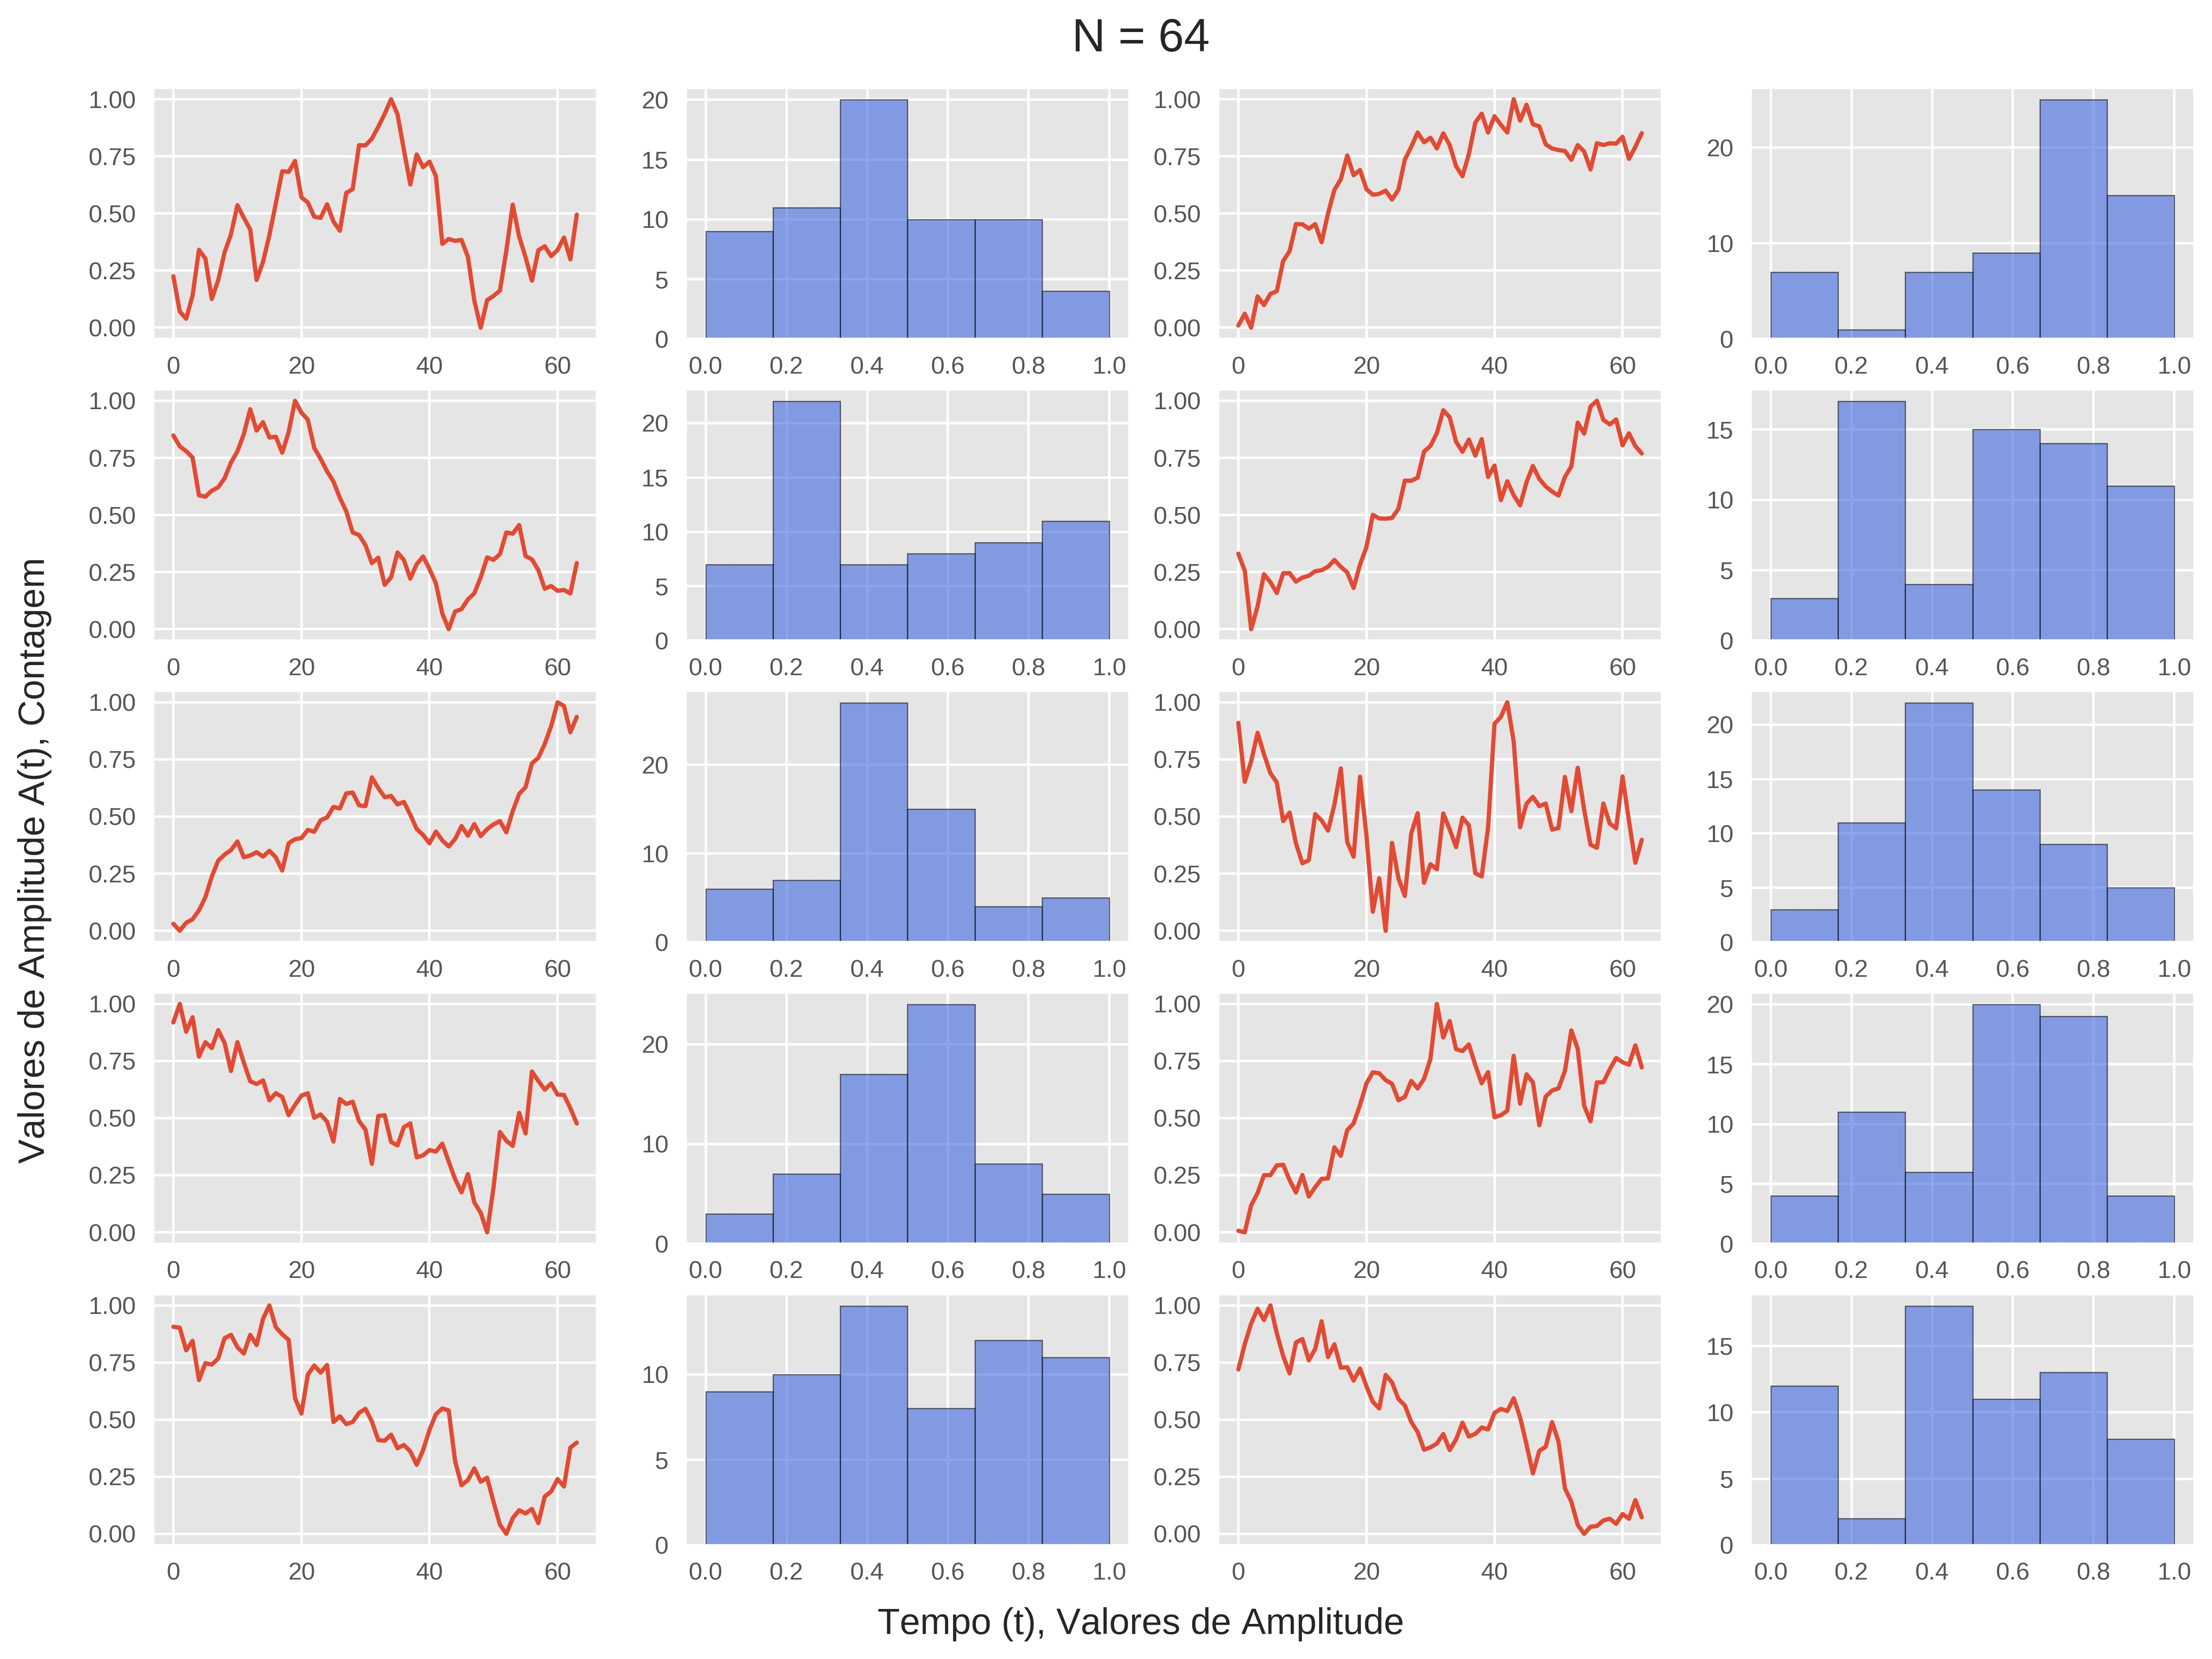
\includegraphics{Figuras/ex1/Exercicio1_n_64.jpg}}		
	\end{center}
	\vspace{-2mm}	% acrescentar o espaçamento vertical apropriado entre a borda inferior da figura e a legenda ou a fonte quando não há legenda (o valor pode ser negativo para subir)
	\legenda{Figura 1.1: Dez sinais e seus respectivos histogramas para  asérie com $N$ = 64 do grupo noise.}	% legenda - para deixar sem legenda usar comando \legenda{} (nunca deve-se comentar o comando \legenda)
	\label{ex1_fig1}
	%\FONTE{}	% fonte consultada (elemento obrigatório, mesmo que seja produção do próprio autor)
\end{figure}

Os resultados da análise foram armazenados em três arquivos .csv: \textit{Exercicio1\_momentos.csv}, contendo os quatro momentos estatísticos de cada sinal gerado, \textit{Exercicio1\_parametros.csv}, com a variância, skewness e kurtosis de todos os sinais, e \textit{Exercicio1\_kmeans.csv}, que armazena o resultado da análise dos clusters via kmeans, com as coordenadas de cada centróide gerado para cada número de cluster testado e suas respectivas inércias. Foram testados de um a oito clusters para as séries da família noise. Os plots a seguir ilustram o resultado da aplicação do algoritmo kmeans\_3D.py no espaço de parâmetros variância x skewness x kurtosis. O método do cotovelo identificou que três clusters são ideais para classificar os sinais desta família.

\begin{figure}[ht!]
	%\caption{Série e histogramas.}
	\vspace{0mm}	% acrescentar o espaçamento vertical apropriado entre o título e a borda superior da figura
	\begin{center}
		\resizebox{16cm}{!}{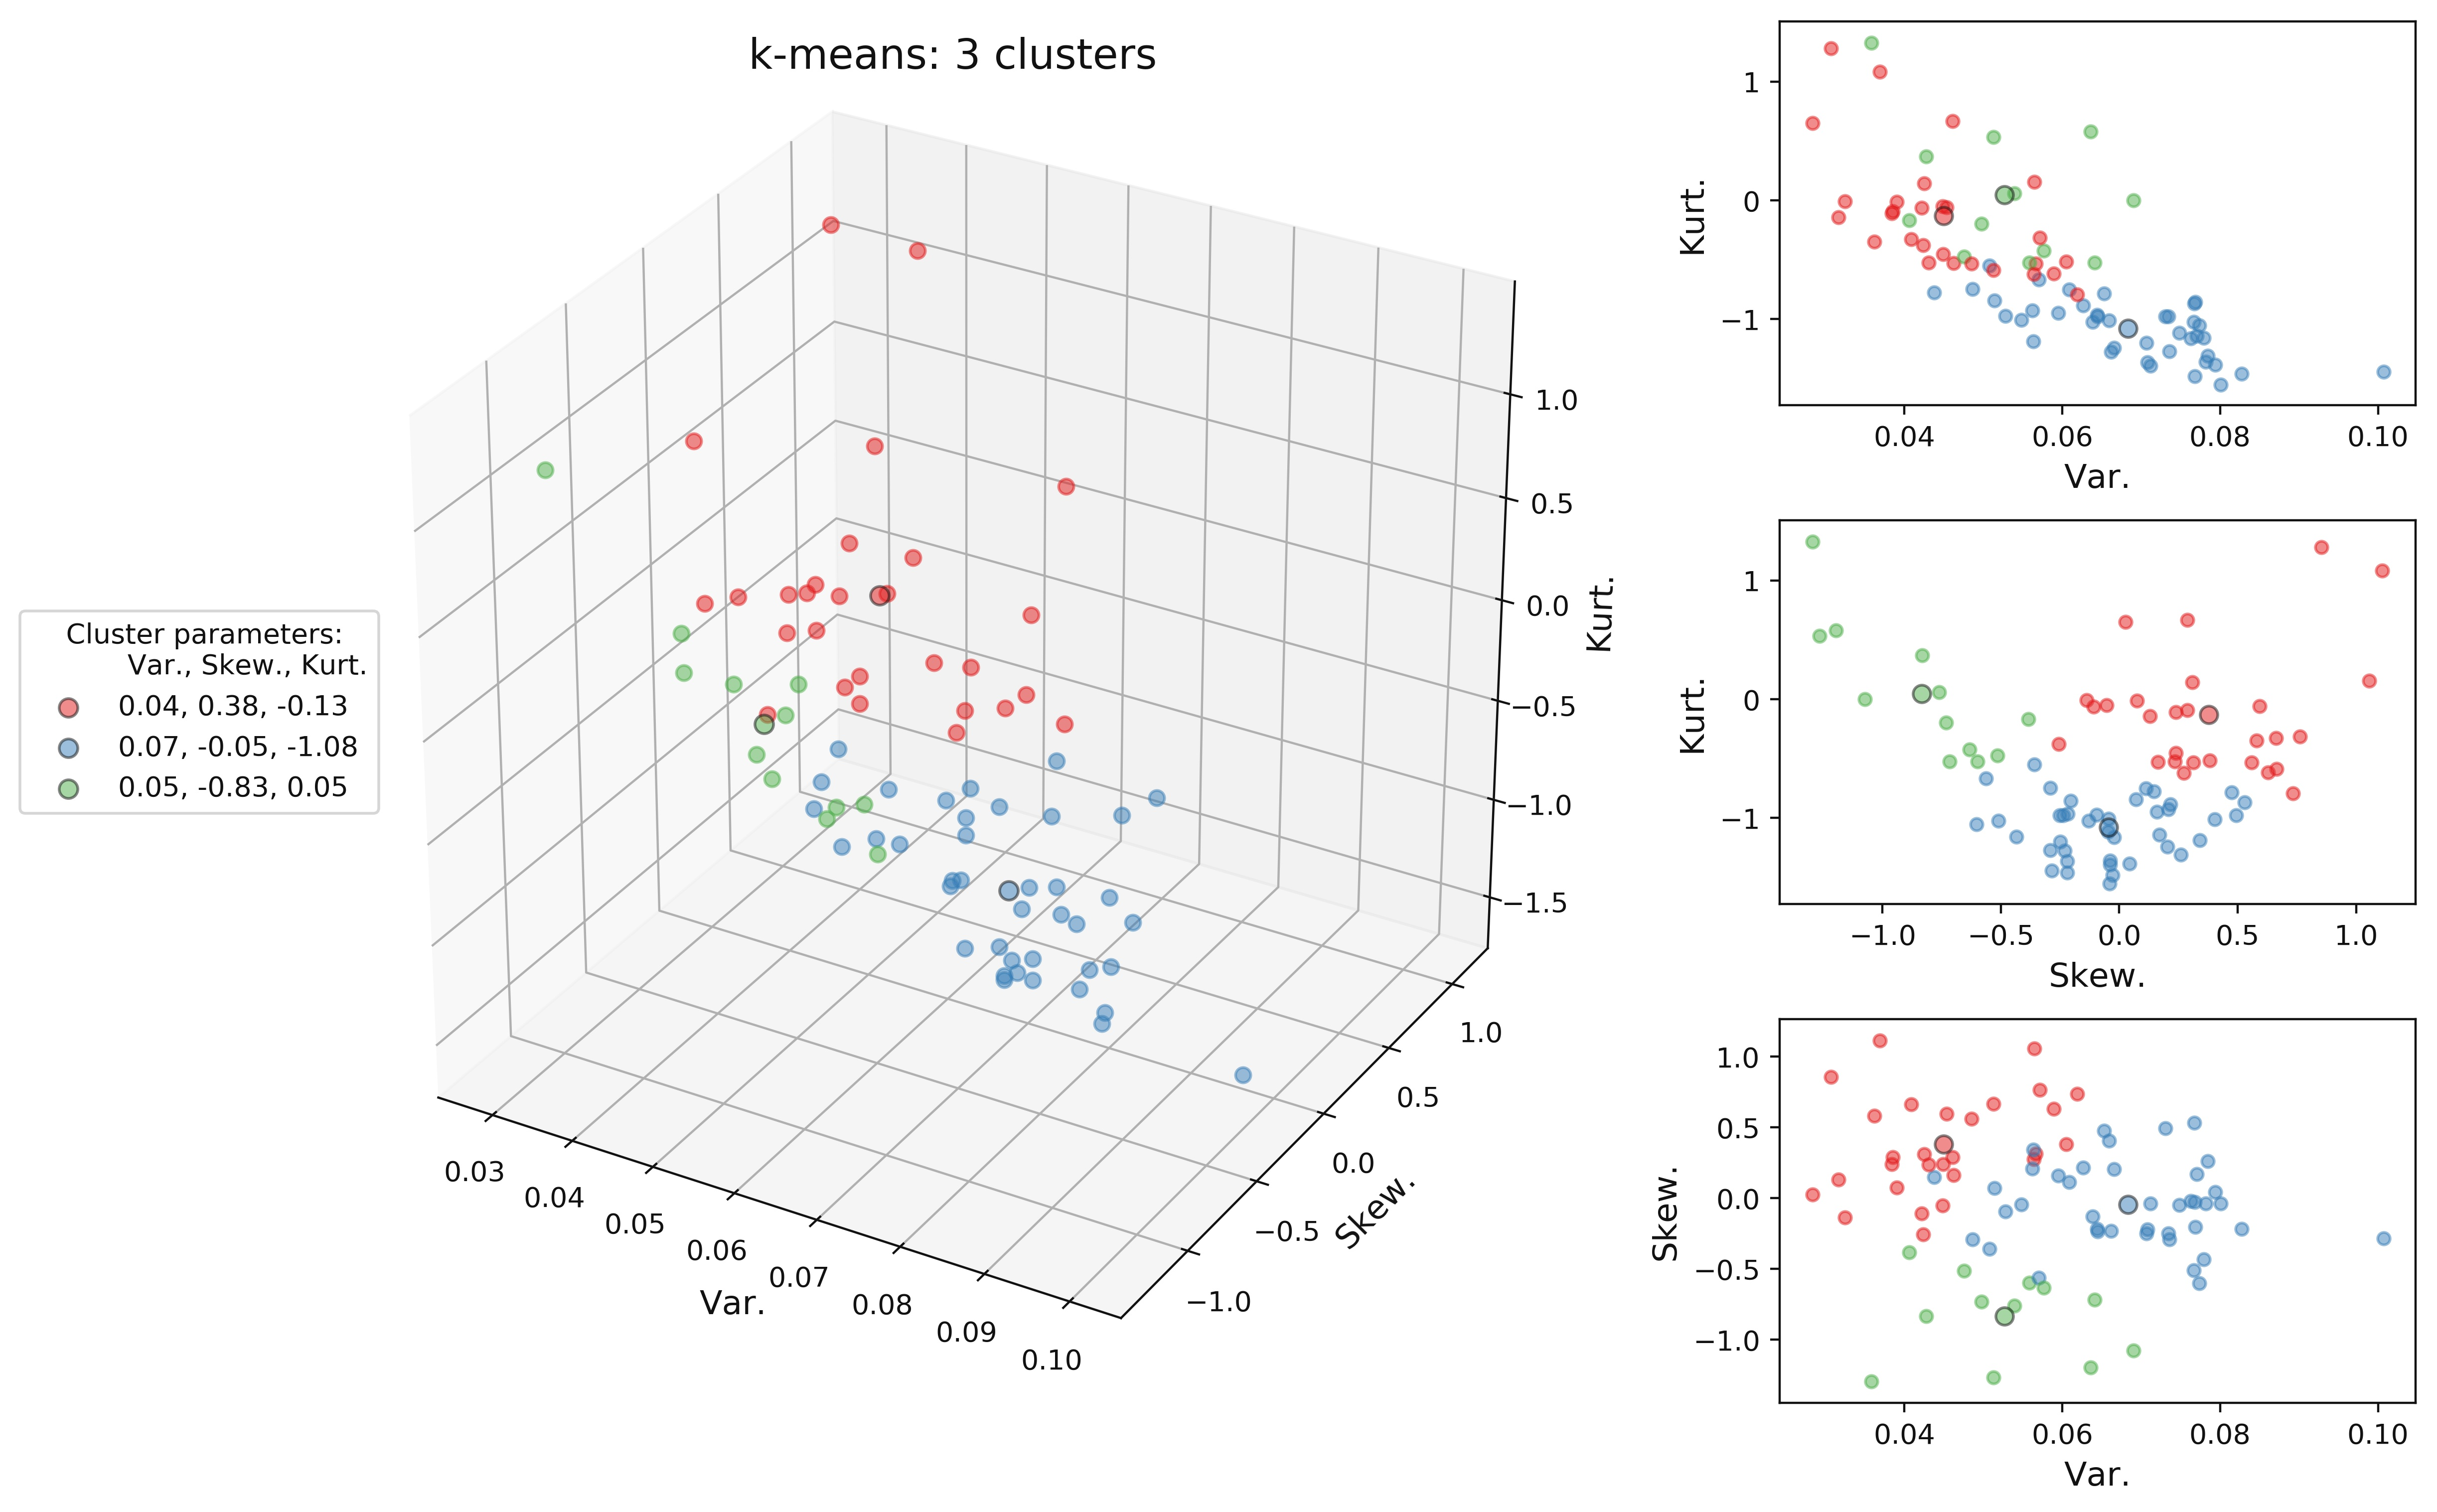
\includegraphics{Figuras/ex1/Exercicio1_cluster_3.jpg}}		
	\end{center}
	\vspace{-2mm}	% acrescentar o espaçamento vertical apropriado entre a borda inferior da figura e a legenda ou a fonte quando não há legenda (o valor pode ser negativo para subir)
	\legenda{Figura 1.2: Técnica kmeans no espaço de parâmetros variância x skewness x kurtosis para a família de sinais noise. Resultado para número de clusters $n\_c$ = 3.}	% legenda - para deixar sem legenda usar comando \legenda{} (nunca deve-se comentar o comando \legenda)
	\label{ex1_fig2}
	%\FONTE{}	% fonte consultada (elemento obrigatório, mesmo que seja produção do próprio autor)
\end{figure}

\begin{figure}[ht!]
	%\caption{Série e histogramas.}
	\vspace{0mm}	% acrescentar o espaçamento vertical apropriado entre o título e a borda superior da figura
	\begin{center}
		\resizebox{11cm}{!}{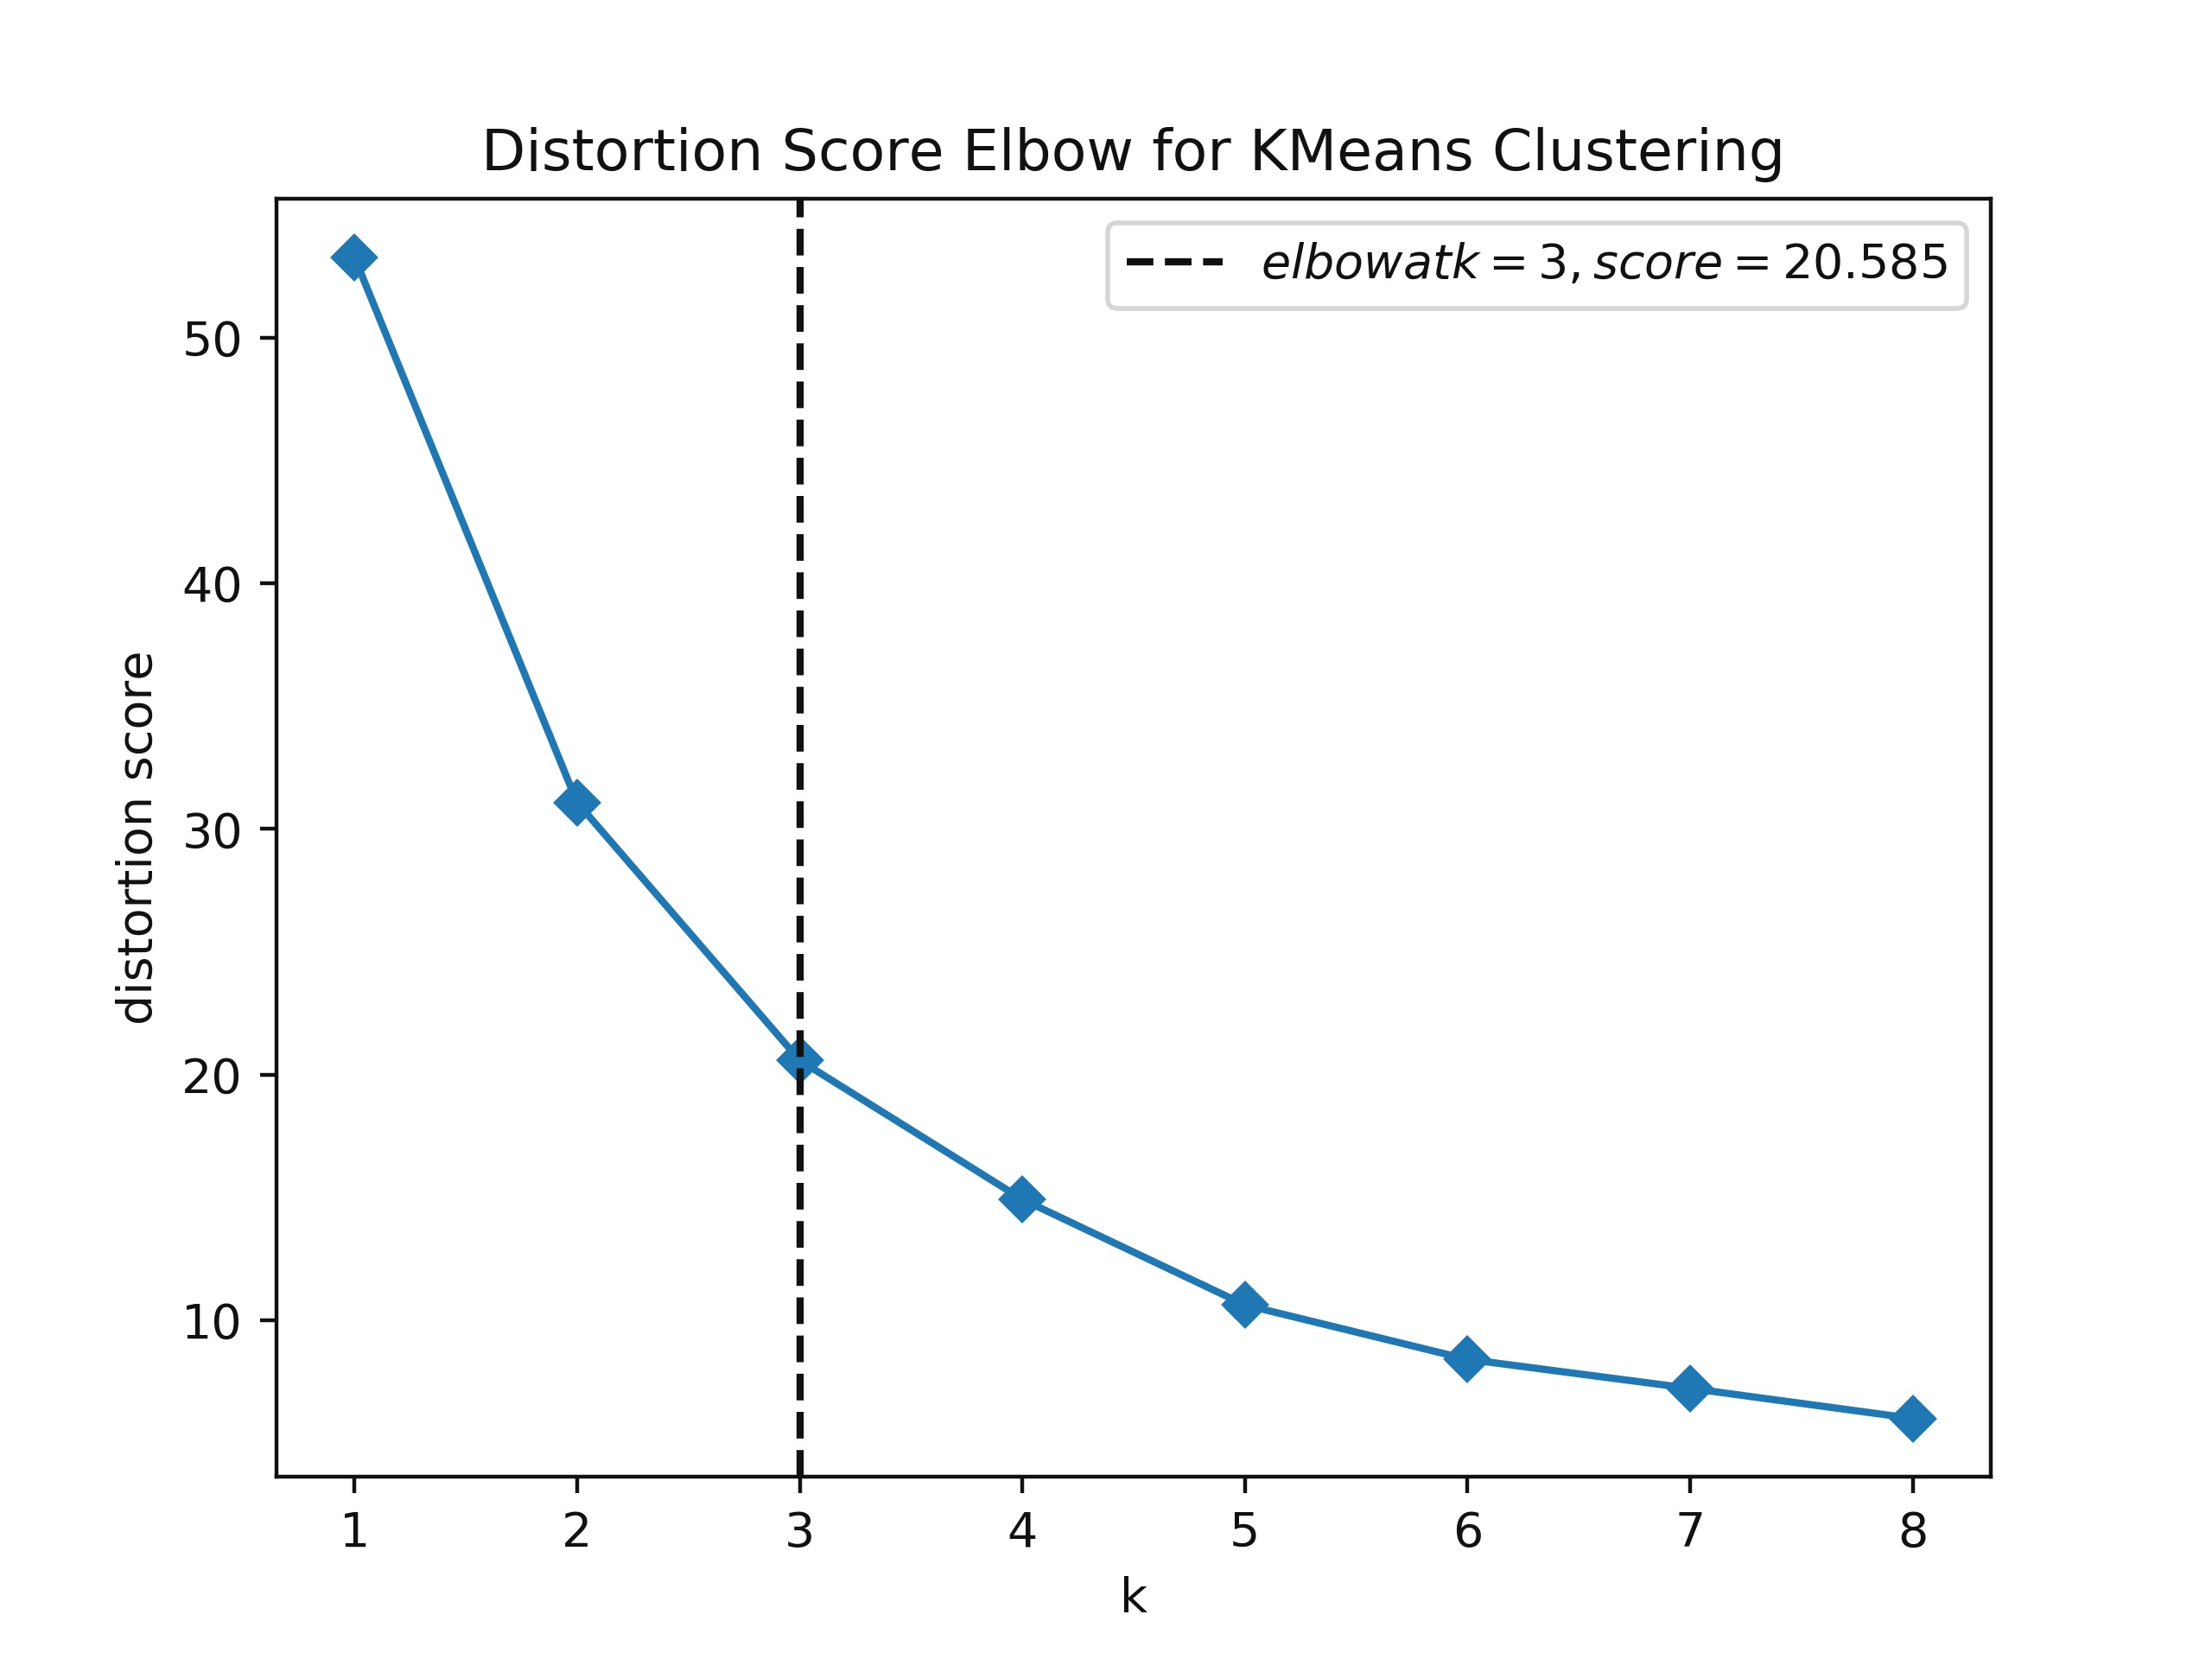
\includegraphics{Figuras/ex1/Exercicio1_elbow_algorithm.jpg}}		
	\end{center}
	\vspace{-2mm}	% acrescentar o espaçamento vertical apropriado entre a borda inferior da figura e a legenda ou a fonte quando não há legenda (o valor pode ser negativo para subir)
	\legenda{Figura 1.3: Resultado do método do cotovelo, com o gráfico de número de clusters x inércia dos centróides. O pacote yellowbric.cluster foi utilizado para determinar o número de clusters ideal.}	% legenda - para deixar sem legenda usar comando \legenda{} (nunca deve-se comentar o comando \legenda)
	\label{ex1_fig3}
	%\FONTE{}	% fonte consultada (elemento obrigatório, mesmo que seja produção do próprio autor)
\end{figure}
%
%\subsection*{1.1}
%\addcontentsline{toc}{section}{\protect\numberline{} 1.1}%

%O script \textit{noise.py}, utilizado para gerar os sinais, se encontra na pasta \textit{signal\_generator\_codes}. Ele tem como input o tamanho da série $n$. Além de gerar as séries, ele também gera o histograma e os respectivos plots, bem como arquivos \textit{momentos.csv} e \textit{parametros.csv} com os valores de todos os momentos estatísticos e parâmetros relevantes para este exercício (variância, skewness e kurtosis).

%\subsection*{1.2}
%\addcontentsline{toc}{section}{\protect\numberline{} 1.2}%

%O script de análise estatística \textit{stats\_tools.py} incorpora funções de normalização e de cálculo dos momentos estatísticos. Ele é importado a partir da pasta \textit{statistical\_analysis\_codes}.

%\subsection*{1.3}
%\addcontentsline{toc}{section}{\protect\numberline{} 1.3}%

%O script \textit{kmeans\_3D.py} analisa qualquer conjunto tridimensional de dados. Além dos dados, o número de clusters a serem testados também é um dos inputs. Ele gera gráficos dos dados no espaço de parâmetros sendo analisado, e determina o melhor número de cluster pelo método do cotovelo. O arquivo \textit{kmeans.csv} gerado pelo script contém informação das coordenadas x, y e z do centróide e da inércia para cada número de cluster testado. No presente exercício 8 clusters foram avaliados. O algoritmo \textit{kmeans\_3D.py} se encontra na pasta \textit{statistical\_analysis\_codes}.
 %% 1o capítulo, começo do texto

\clearpage
%%%%%%%%%%%%%%%%%%%%%%%%%%%%%%%%%%%%%%%%%%%%%%%%%%%%%%%%%%%%%%%%%%%%%%%%%%%%%%%

\section*{\large Exercício 2 - Repita o exercício anterior considerando, entretanto, o algoritmo colorednoise.py}
\addcontentsline{toc}{chapter}{\protect\numberline{}\large Exercício 2}%

Os resultados das análises dos sinais referentes a este exercício se encontram na pasta \textbf{Exercise2}. O plot a seguir ilustra vinte sinais gerados para a família colornoise com $\beta$ = 2, representando ruído marrom. 

%[angle=90]
\begin{figure}[ht!]
  \begin{adjustbox}{addcode={\begin{minipage}{\width}}{\\% 
      Figura 2.1: Série de 20 sinais diferentes gerados com o script colornoise.py. Ao todo neste exercício, três valores de $\beta$ foram implementados: 0, gerando ruído branco, 1, do ruído rosa, e 2, representando ruído marrom, todas com tamanho da série igual a 8192. A figura exibe o resultado do ruído marrom e seus respectivos histogramas.
      \end{minipage}},rotate=90,center}
      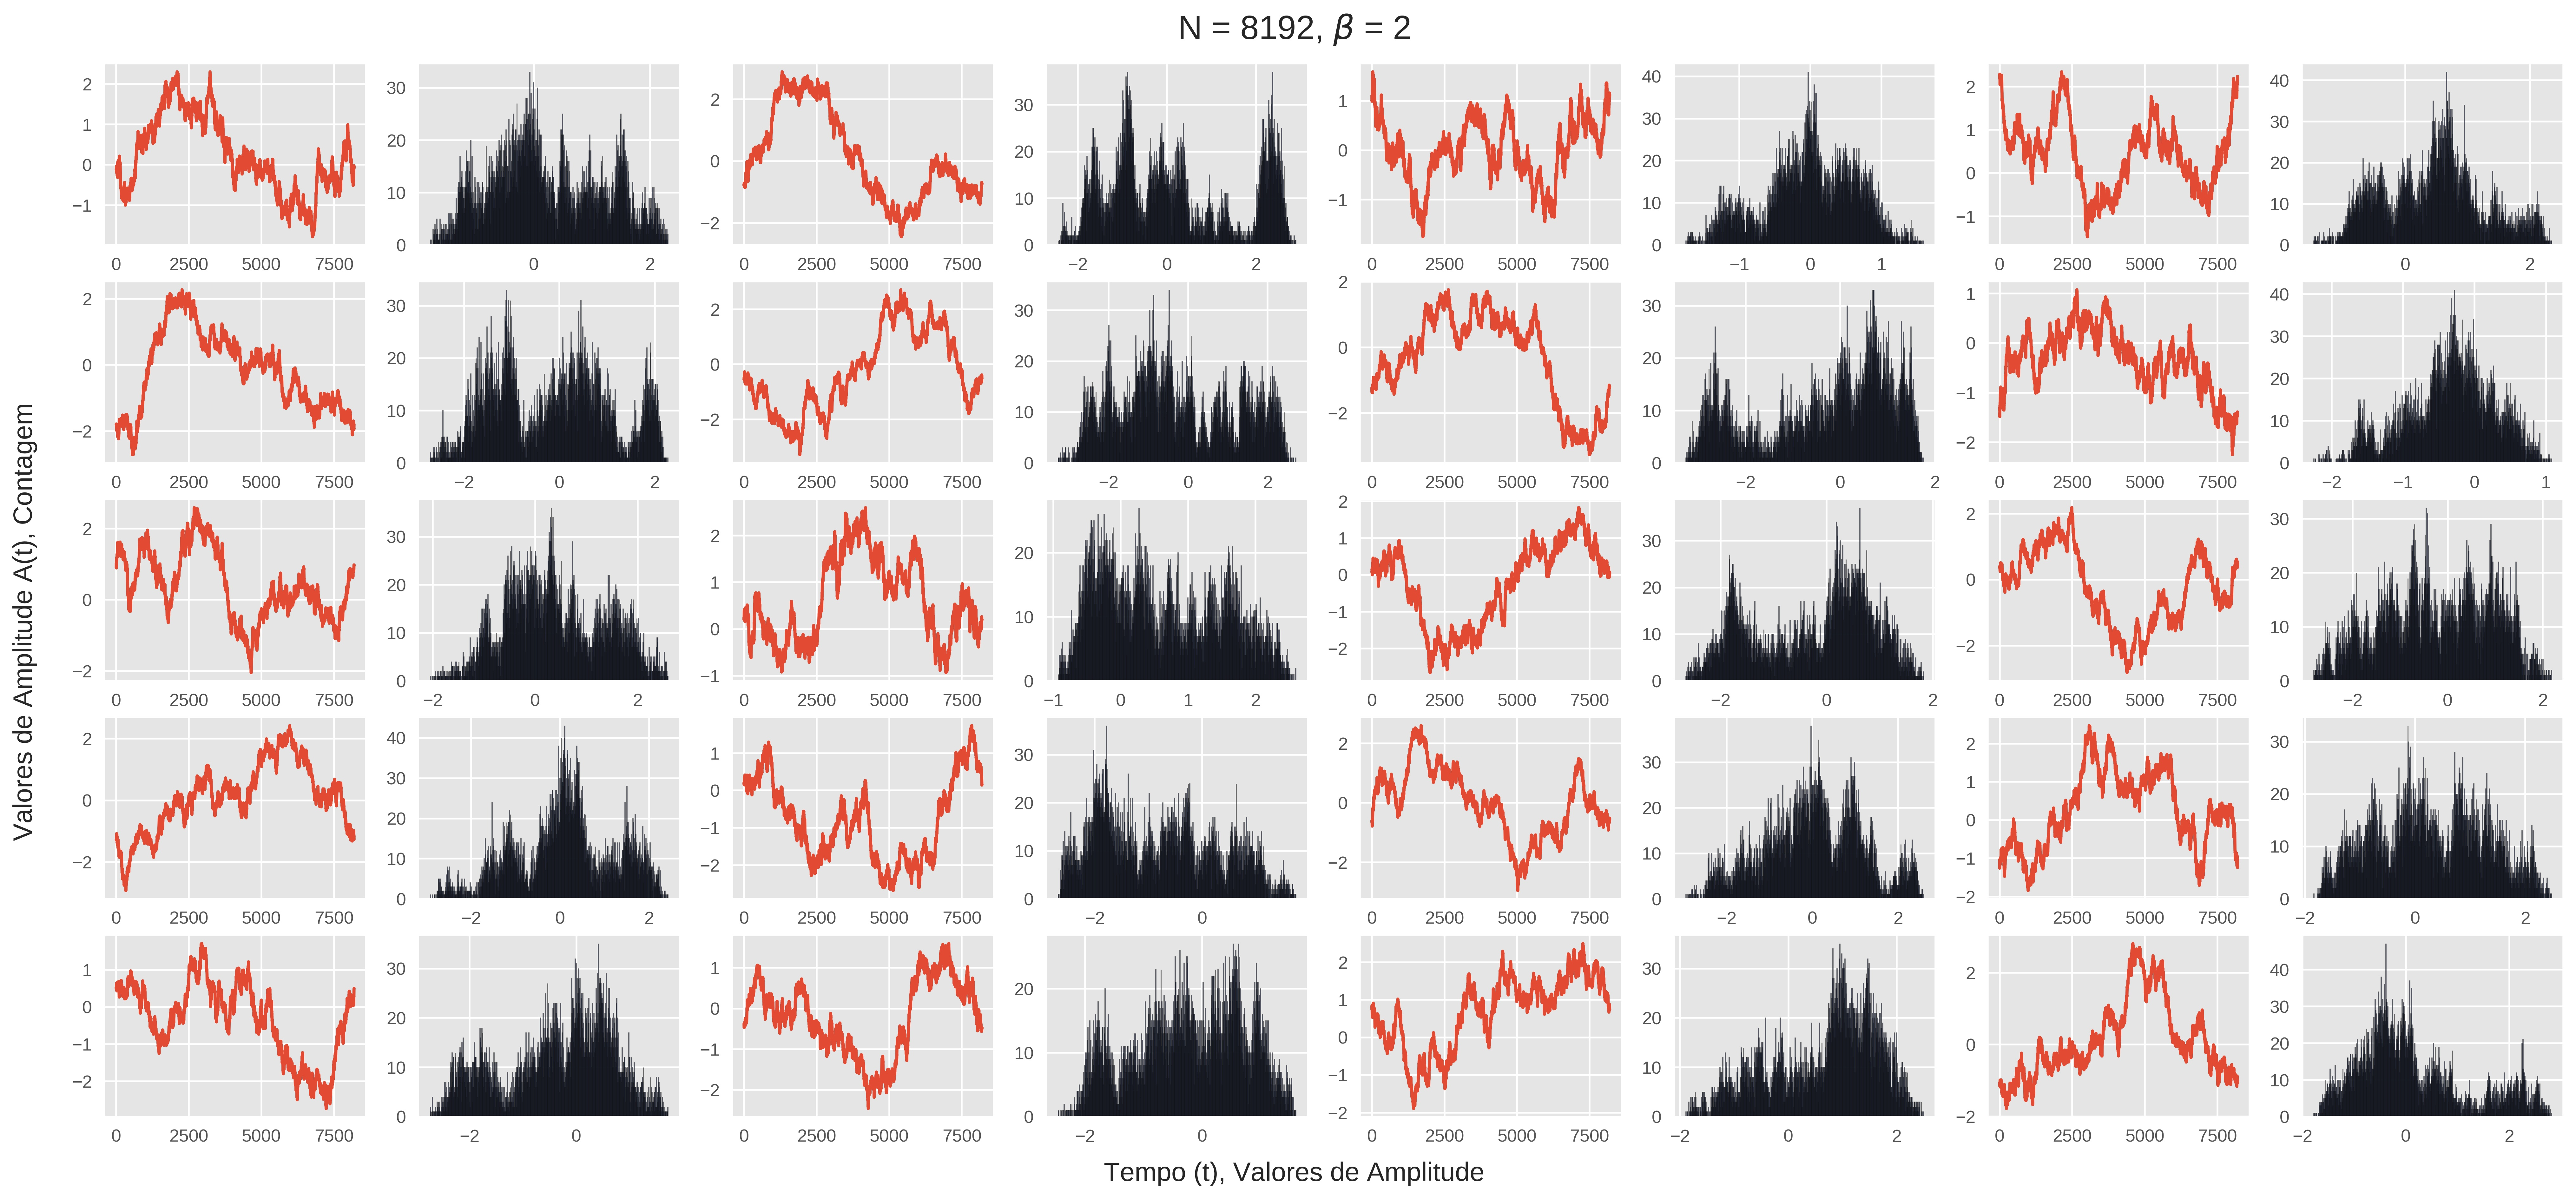
\includegraphics[scale=.35]{Figuras/ex2/Exercicio2_n_8192_beta_2.jpg}	%
  \end{adjustbox}
\end{figure}

%\begin{sidewaysfigure}[ht!]
	%\caption{Série e histogramas.}
	%\vspace{0mm}	% acrescentar o espaçamento vertical apropriado entre o título e a borda superior da figura
	%\begin{center}
%		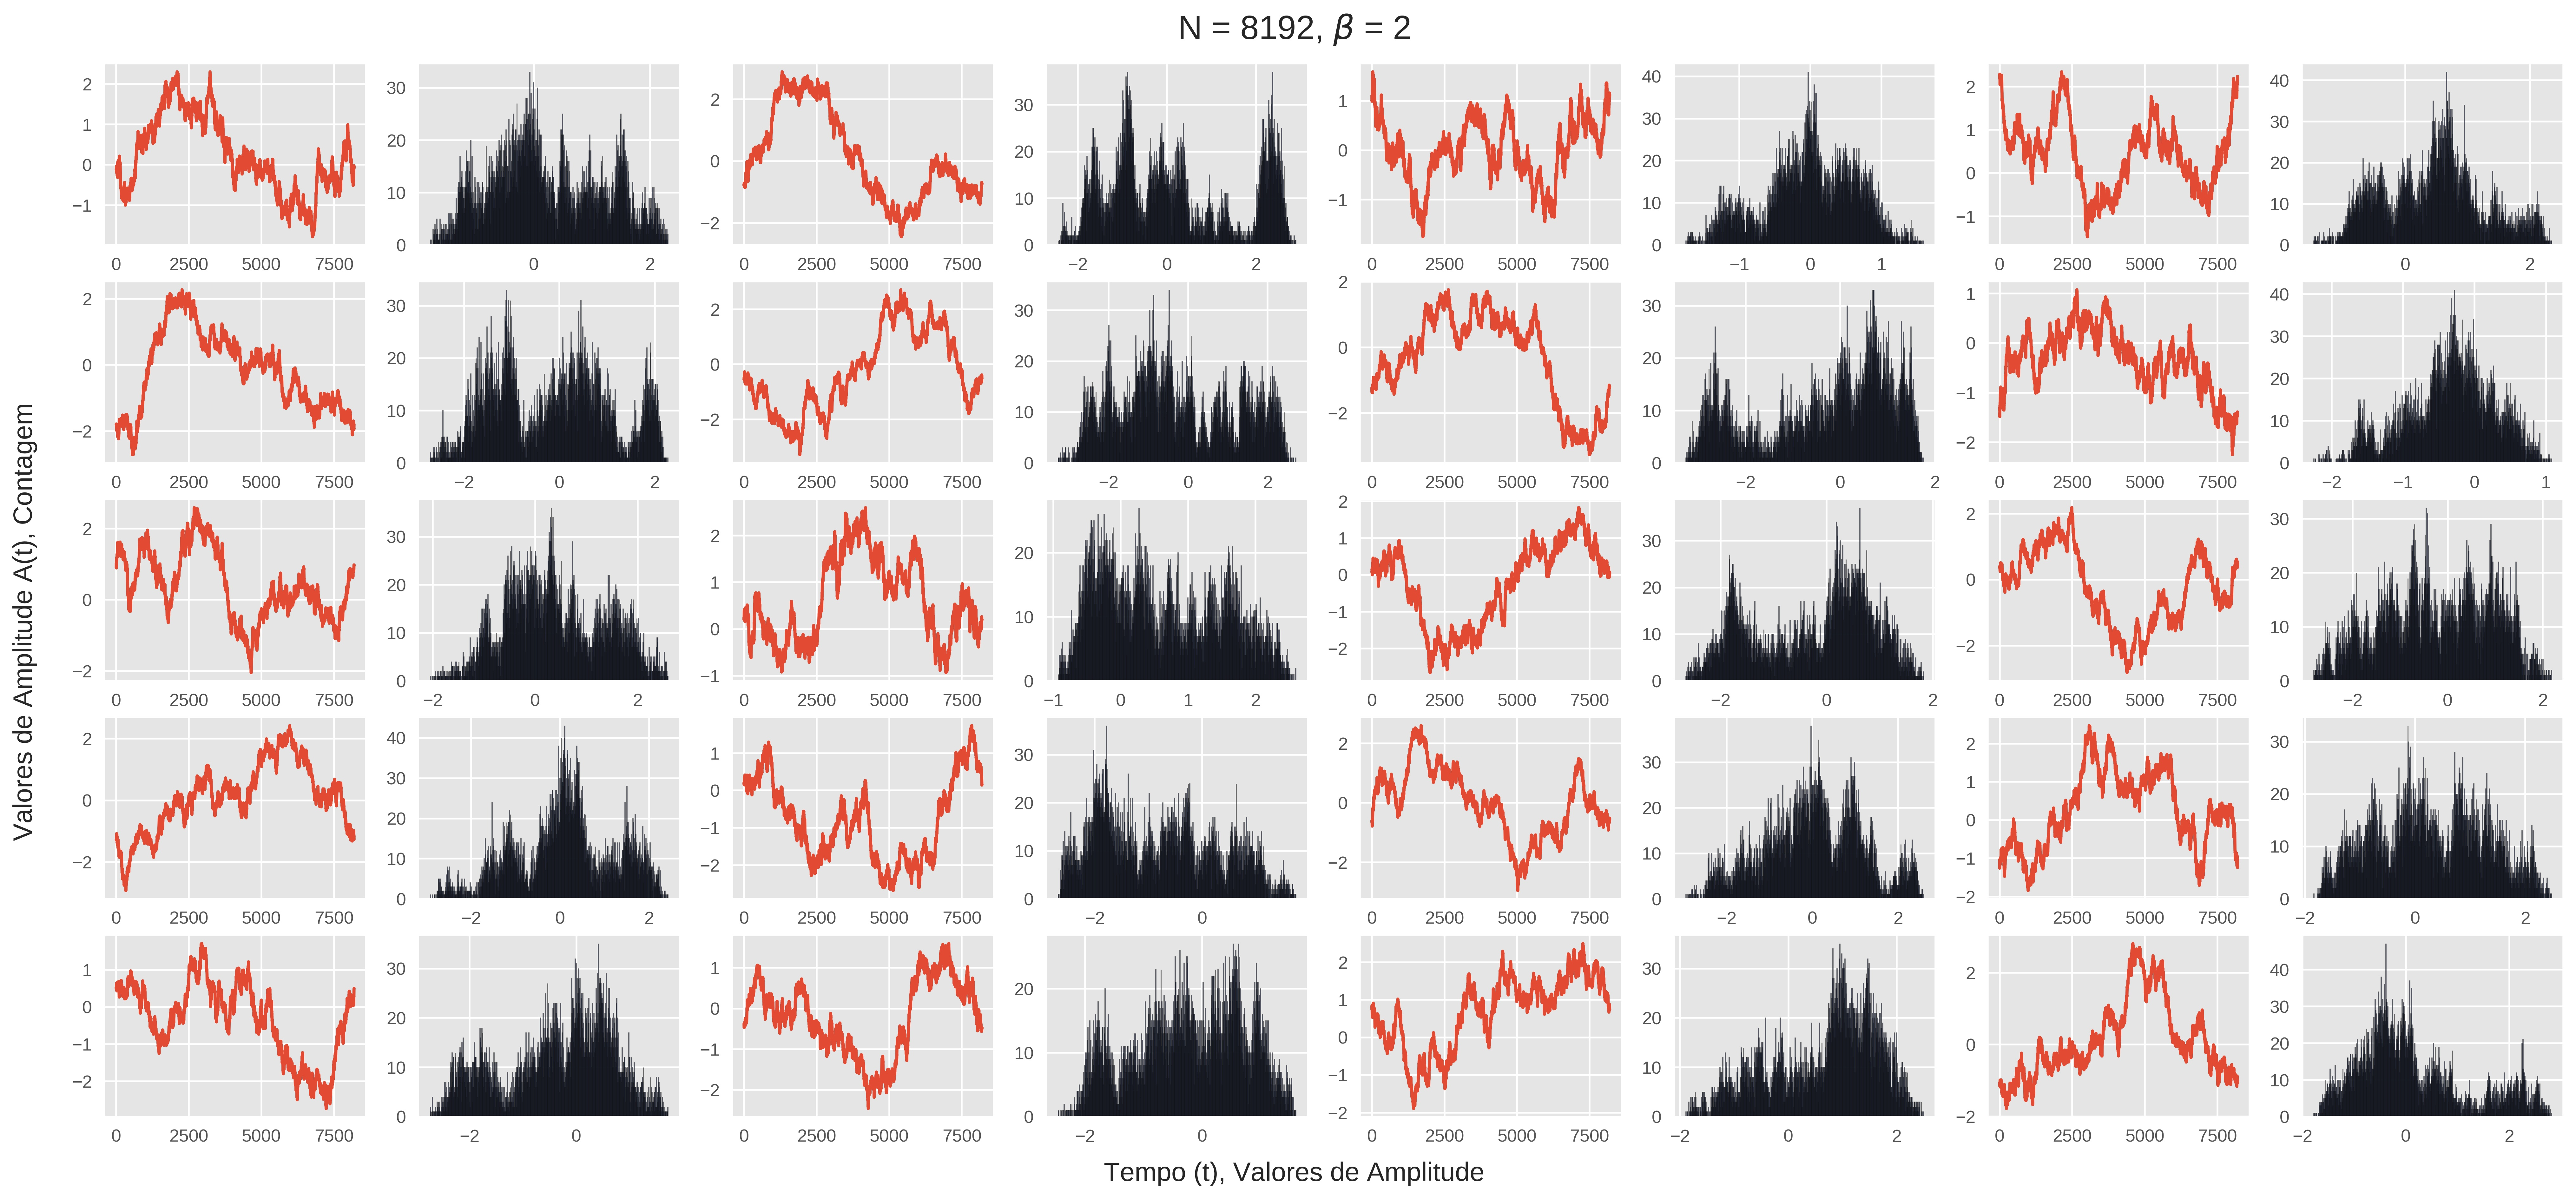
\includegraphics[scale=.3]{Figuras/ex2/Exercicio2_n_8192_beta_2.jpg}	
	%\end{center}
	%\vspace{-2mm}	% acrescentar o espaçamento vertical apropriado entre a borda inferior da figura e a legenda ou a fonte quando não há legenda (o valor pode ser negativo para subir)
%	\legenda{Figura 2.1:.}	% legenda - para deixar sem legenda usar comando \legenda{} (nunca deve-se comentar o comando \legenda)
%	\label{ex2_fig1}
	%\FONTE{}	% fonte consultada (elemento obrigatório, mesmo que seja produção do próprio autor)
%\end{sidewaysfigure}
\clearpage
Os mesmos arquivos .csv gerados na primeira questão foram também gerados para a família colornois: \textit{Exercicio2\_momentos.csv},  \textit{Exercicio2\_parametros.csv} e \textit{Exercicio2\_kmeans.csv}. Os resultados do agrupamento via kmeans são exibidos a seguir.

\begin{figure}[ht!]
	%\caption{Série e histogramas.}
	\vspace{0mm}	% acrescentar o espaçamento vertical apropriado entre o título e a borda superior da figura
	\begin{center}
		\resizebox{15cm}{!}{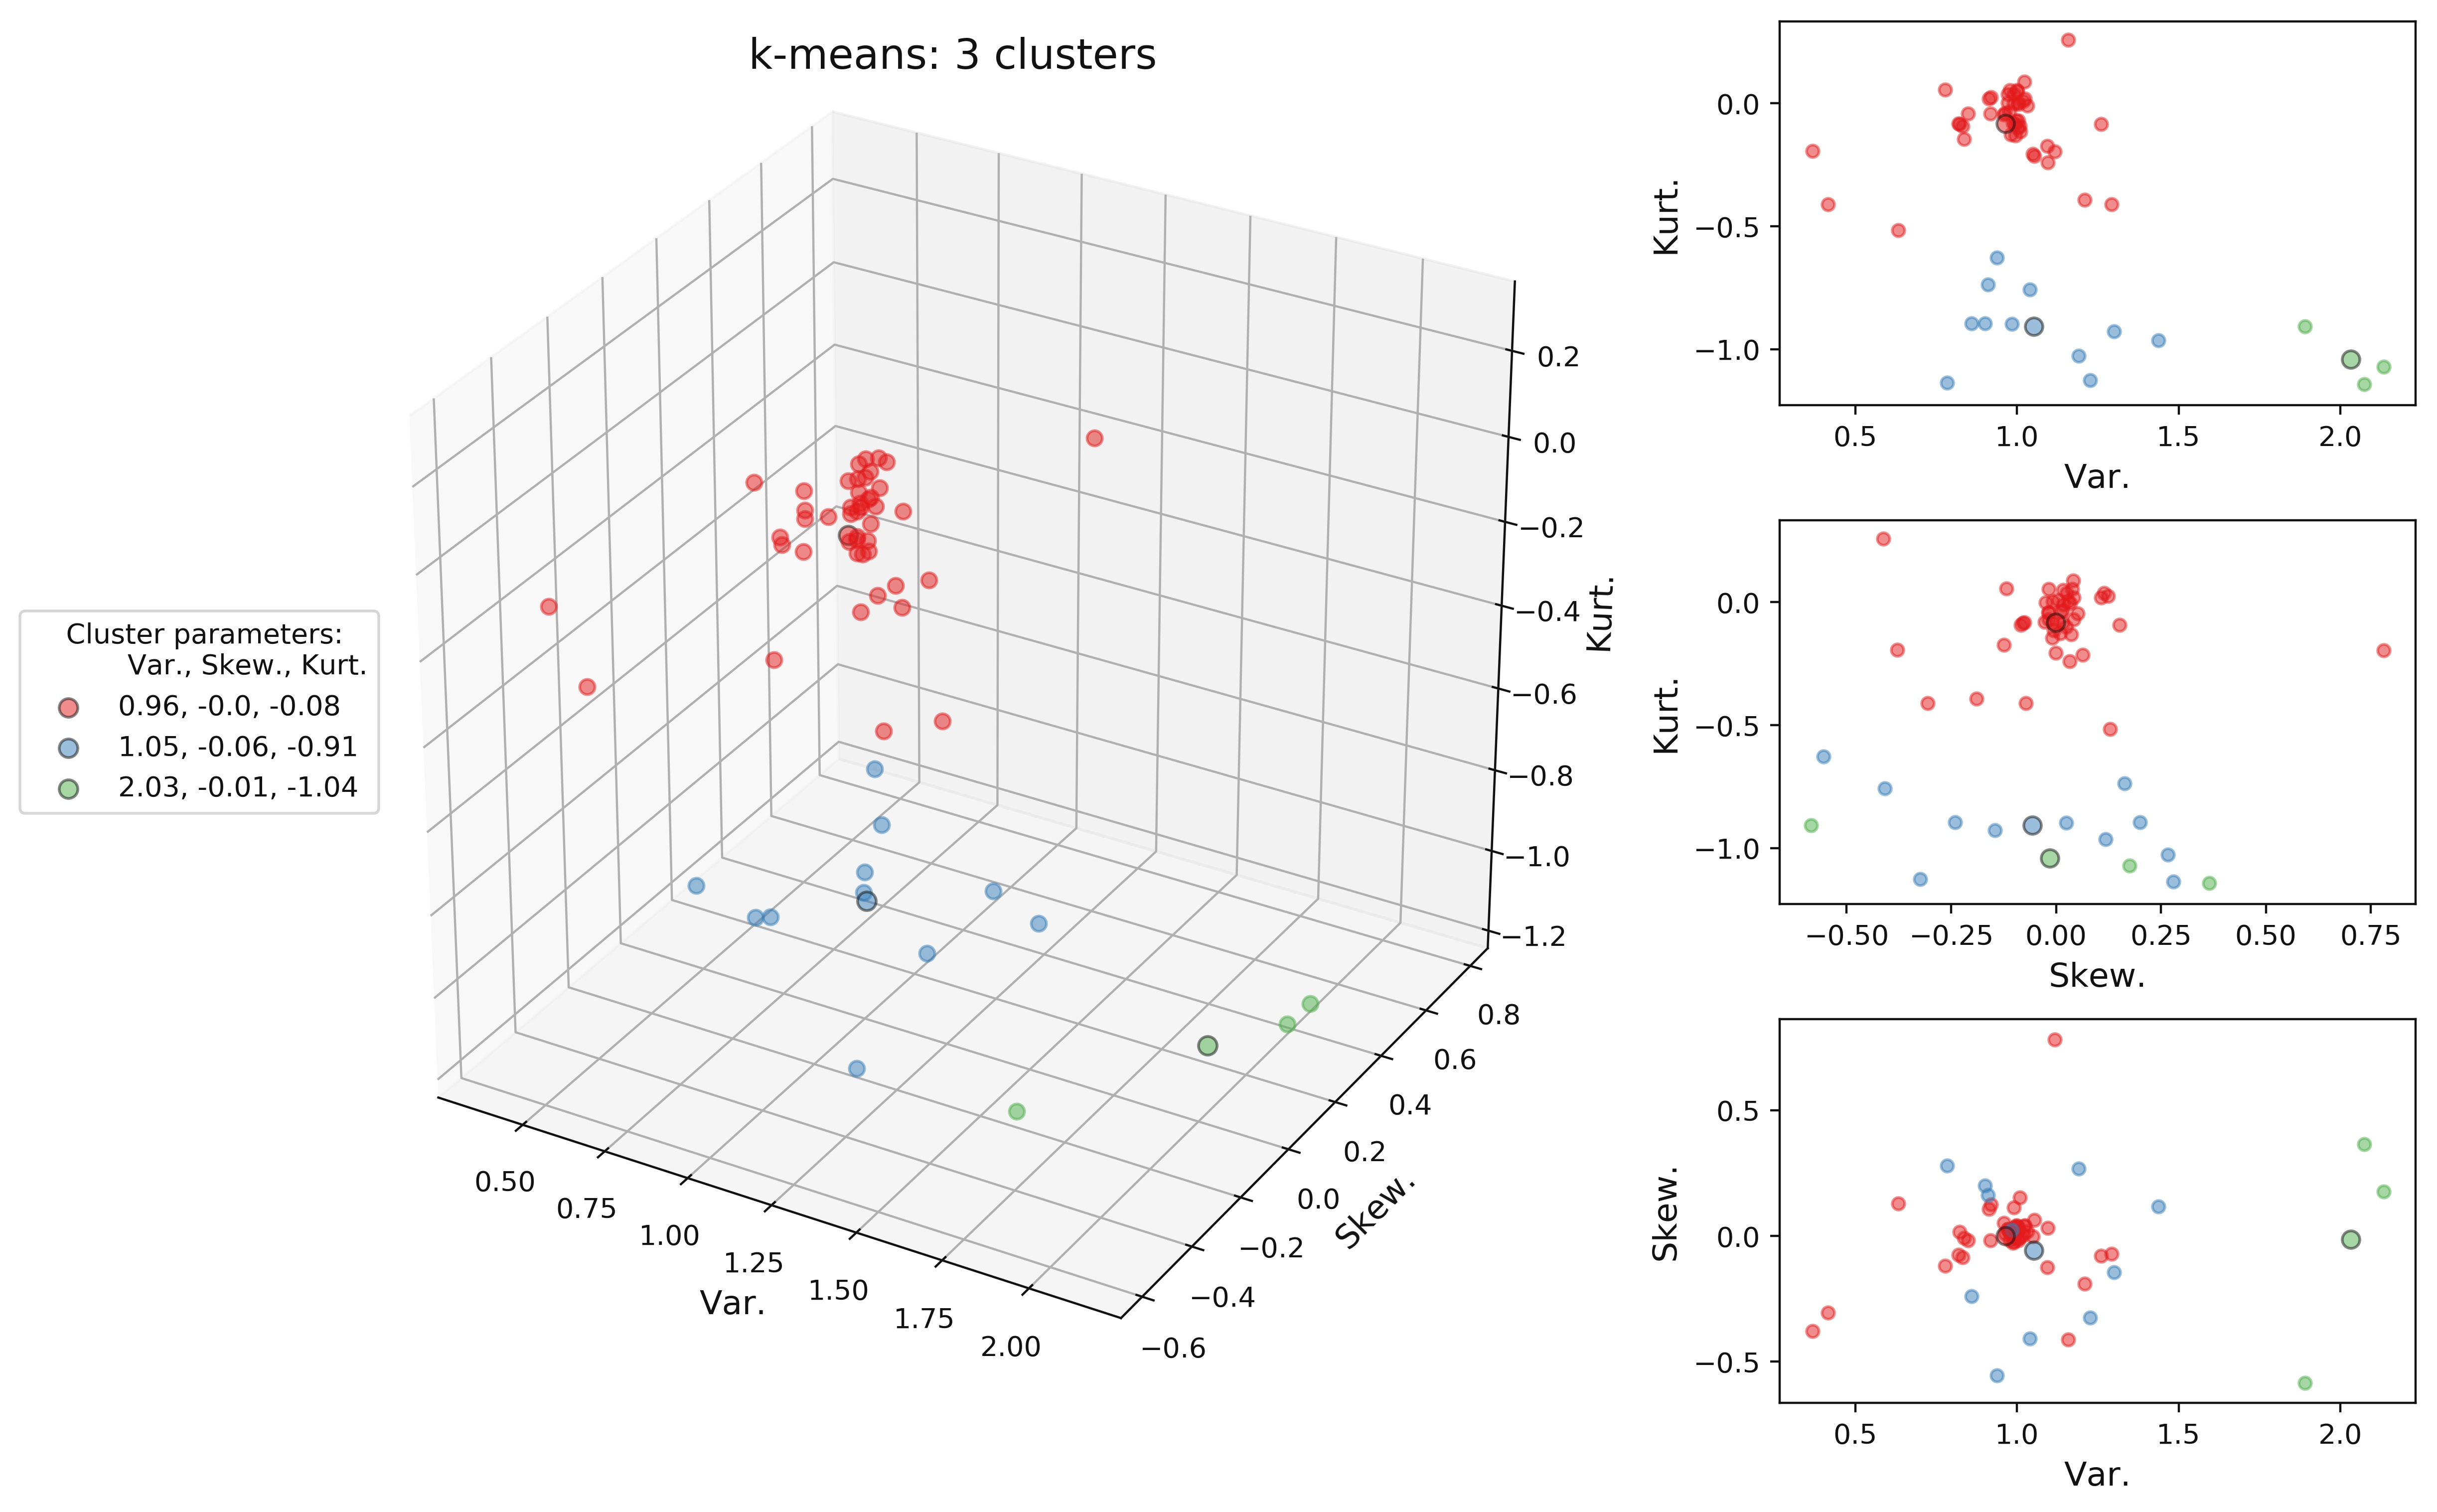
\includegraphics{Figuras/ex2/Exercicio2_cluster_3.jpg}}		
	\end{center}
	\vspace{-3mm}	% acrescentar o espaçamento vertical apropriado entre a borda inferior da figura e a legenda ou a fonte quando não há legenda (o valor pode ser negativo para subir)
	\legenda{Figura 2.2: Técnica kmeans no espaço de parâmetros variância x skewness x kurtosis para a família de sinais colornoise. Resultado para número de clusters $n\_c$ = 3.}	% legenda - para deixar sem legenda usar comando \legenda{} (nunca deve-se comentar o comando \legenda)
	\label{ex2_fig2}
	%\FONTE{}	% fonte consultada (elemento obrigatório, mesmo que seja produção do próprio autor)
\end{figure}

\begin{figure}[ht!]
	%\caption{Série e histogramas.}
	\vspace{0mm}	% acrescentar o espaçamento vertical apropriado entre o título e a borda superior da figura
	\begin{center}
		\resizebox{11cm}{!}{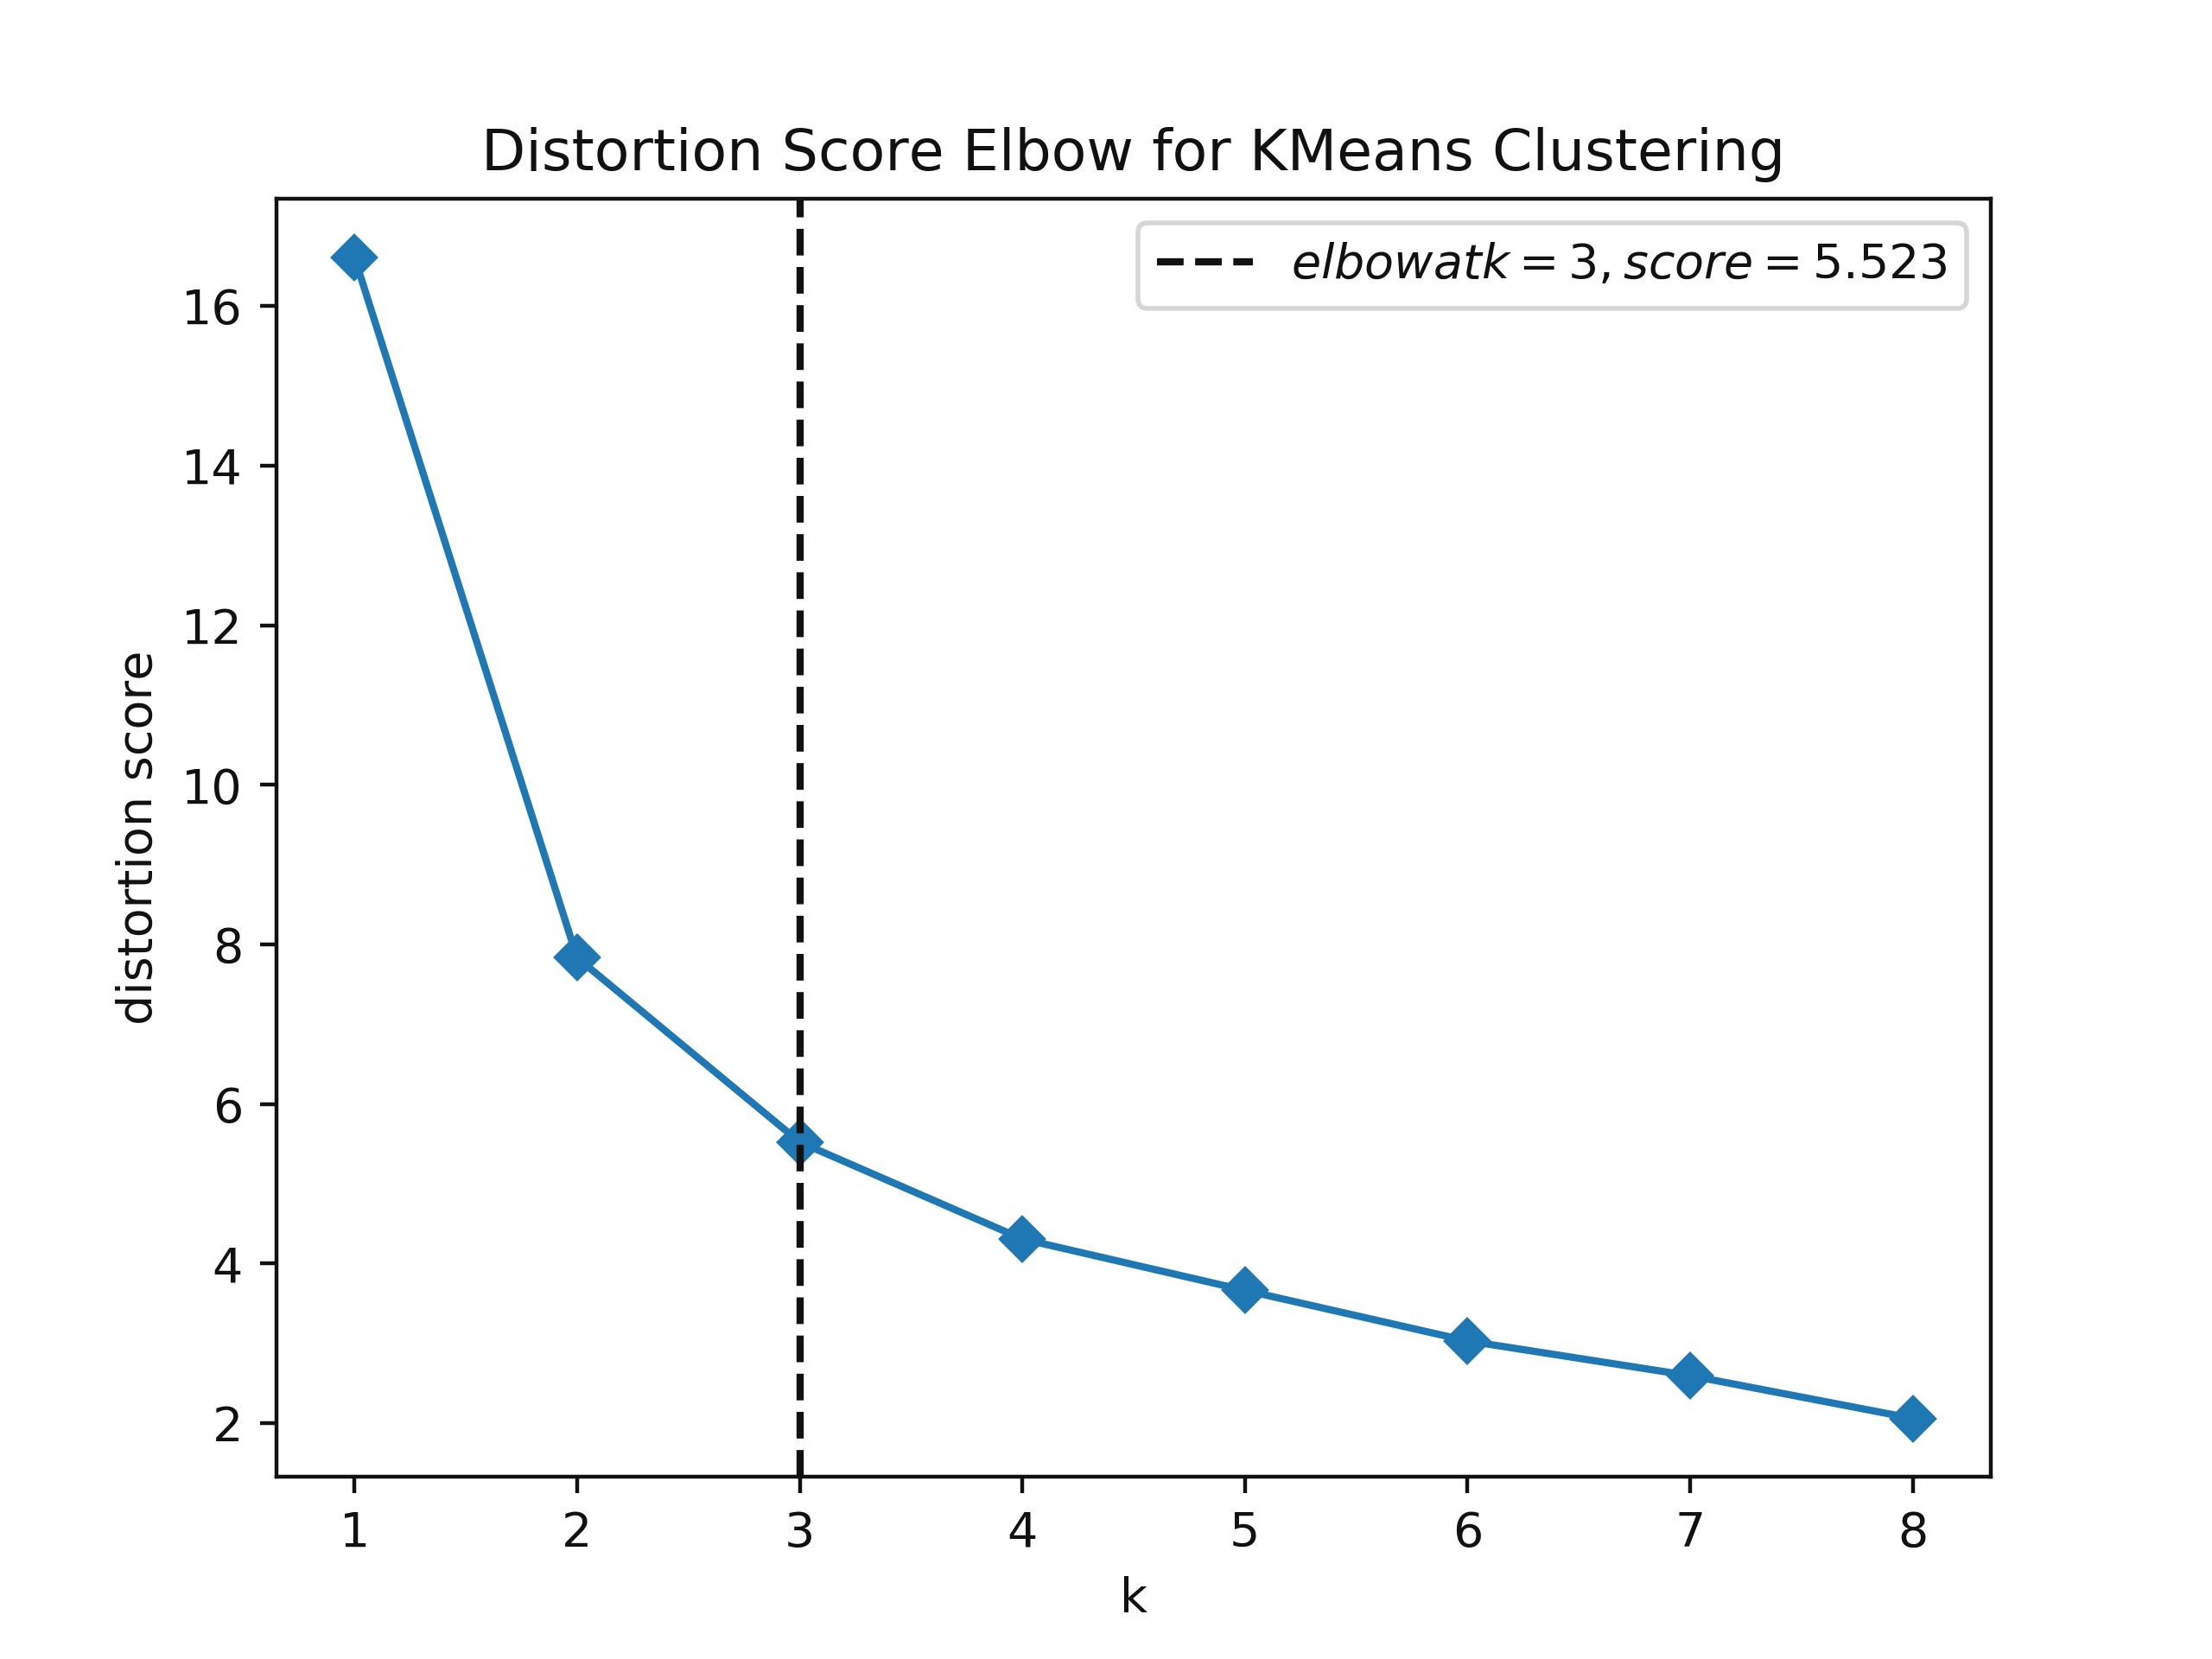
\includegraphics{Figuras/ex2/Exercicio2_elbow_algorithm.jpg}}		
	\end{center}
	\vspace{-3mm}	% acrescentar o espaçamento vertical apropriado entre a borda inferior da figura e a legenda ou a fonte quando não há legenda (o valor pode ser negativo para subir)
	\legenda{Figura 2.3: Resultado do método do cotovelo, mostrando que três clusters são necessários para agrupamento da família colornoise no espaço de parâmetros considerado.}	% legenda - para deixar sem legenda usar comando \legenda{} (nunca deve-se comentar o comando \legenda)
	\label{ex2_fig3}
	%\FONTE{}	% fonte consultada (elemento obrigatório, mesmo que seja produção do próprio autor)
\end{figure} %% 2o capítulo

\clearpage
%%%%%%%%%%%%%%%%%%%%%%%%%%%%%%%%%%%%%%%%%%%%%%%%%%%%%%%%%%%%%%%%%%%%%%%%%%%%%%%

\section*{\large Exercício 3 - Repita o exercício anterior considerando, entretanto, o algoritmo pmodel.py}
\addcontentsline{toc}{chapter}{\protect\numberline{}\large Exercício 3}%

Os resultados das análises dos sinais referentes a este exercício se encontram na pasta \textbf{Exercise3}. Os valores de $\rho$ da família pmnoise foram .18, .23, .28, .32, .37 e .42, onde os três primeiros representam uma série exógena (com parâmetro $\beta$ = 0.7), e os três últimos representam uma série endógena (com parâmetro $\beta$ = 0.4). Todas as séries foram geradas com tamanho igual a 8192. Os plots abaixo ilustram alguns dos resultados para a série exógena e endógena, respectivamente.

\begin{figure}[ht!]
	%\caption{Série e histogramas.}
	\vspace{0mm}	% acrescentar o espaçamento vertical apropriado entre o título e a borda superior da figura
	\begin{center}
		\resizebox{16cm}{!}{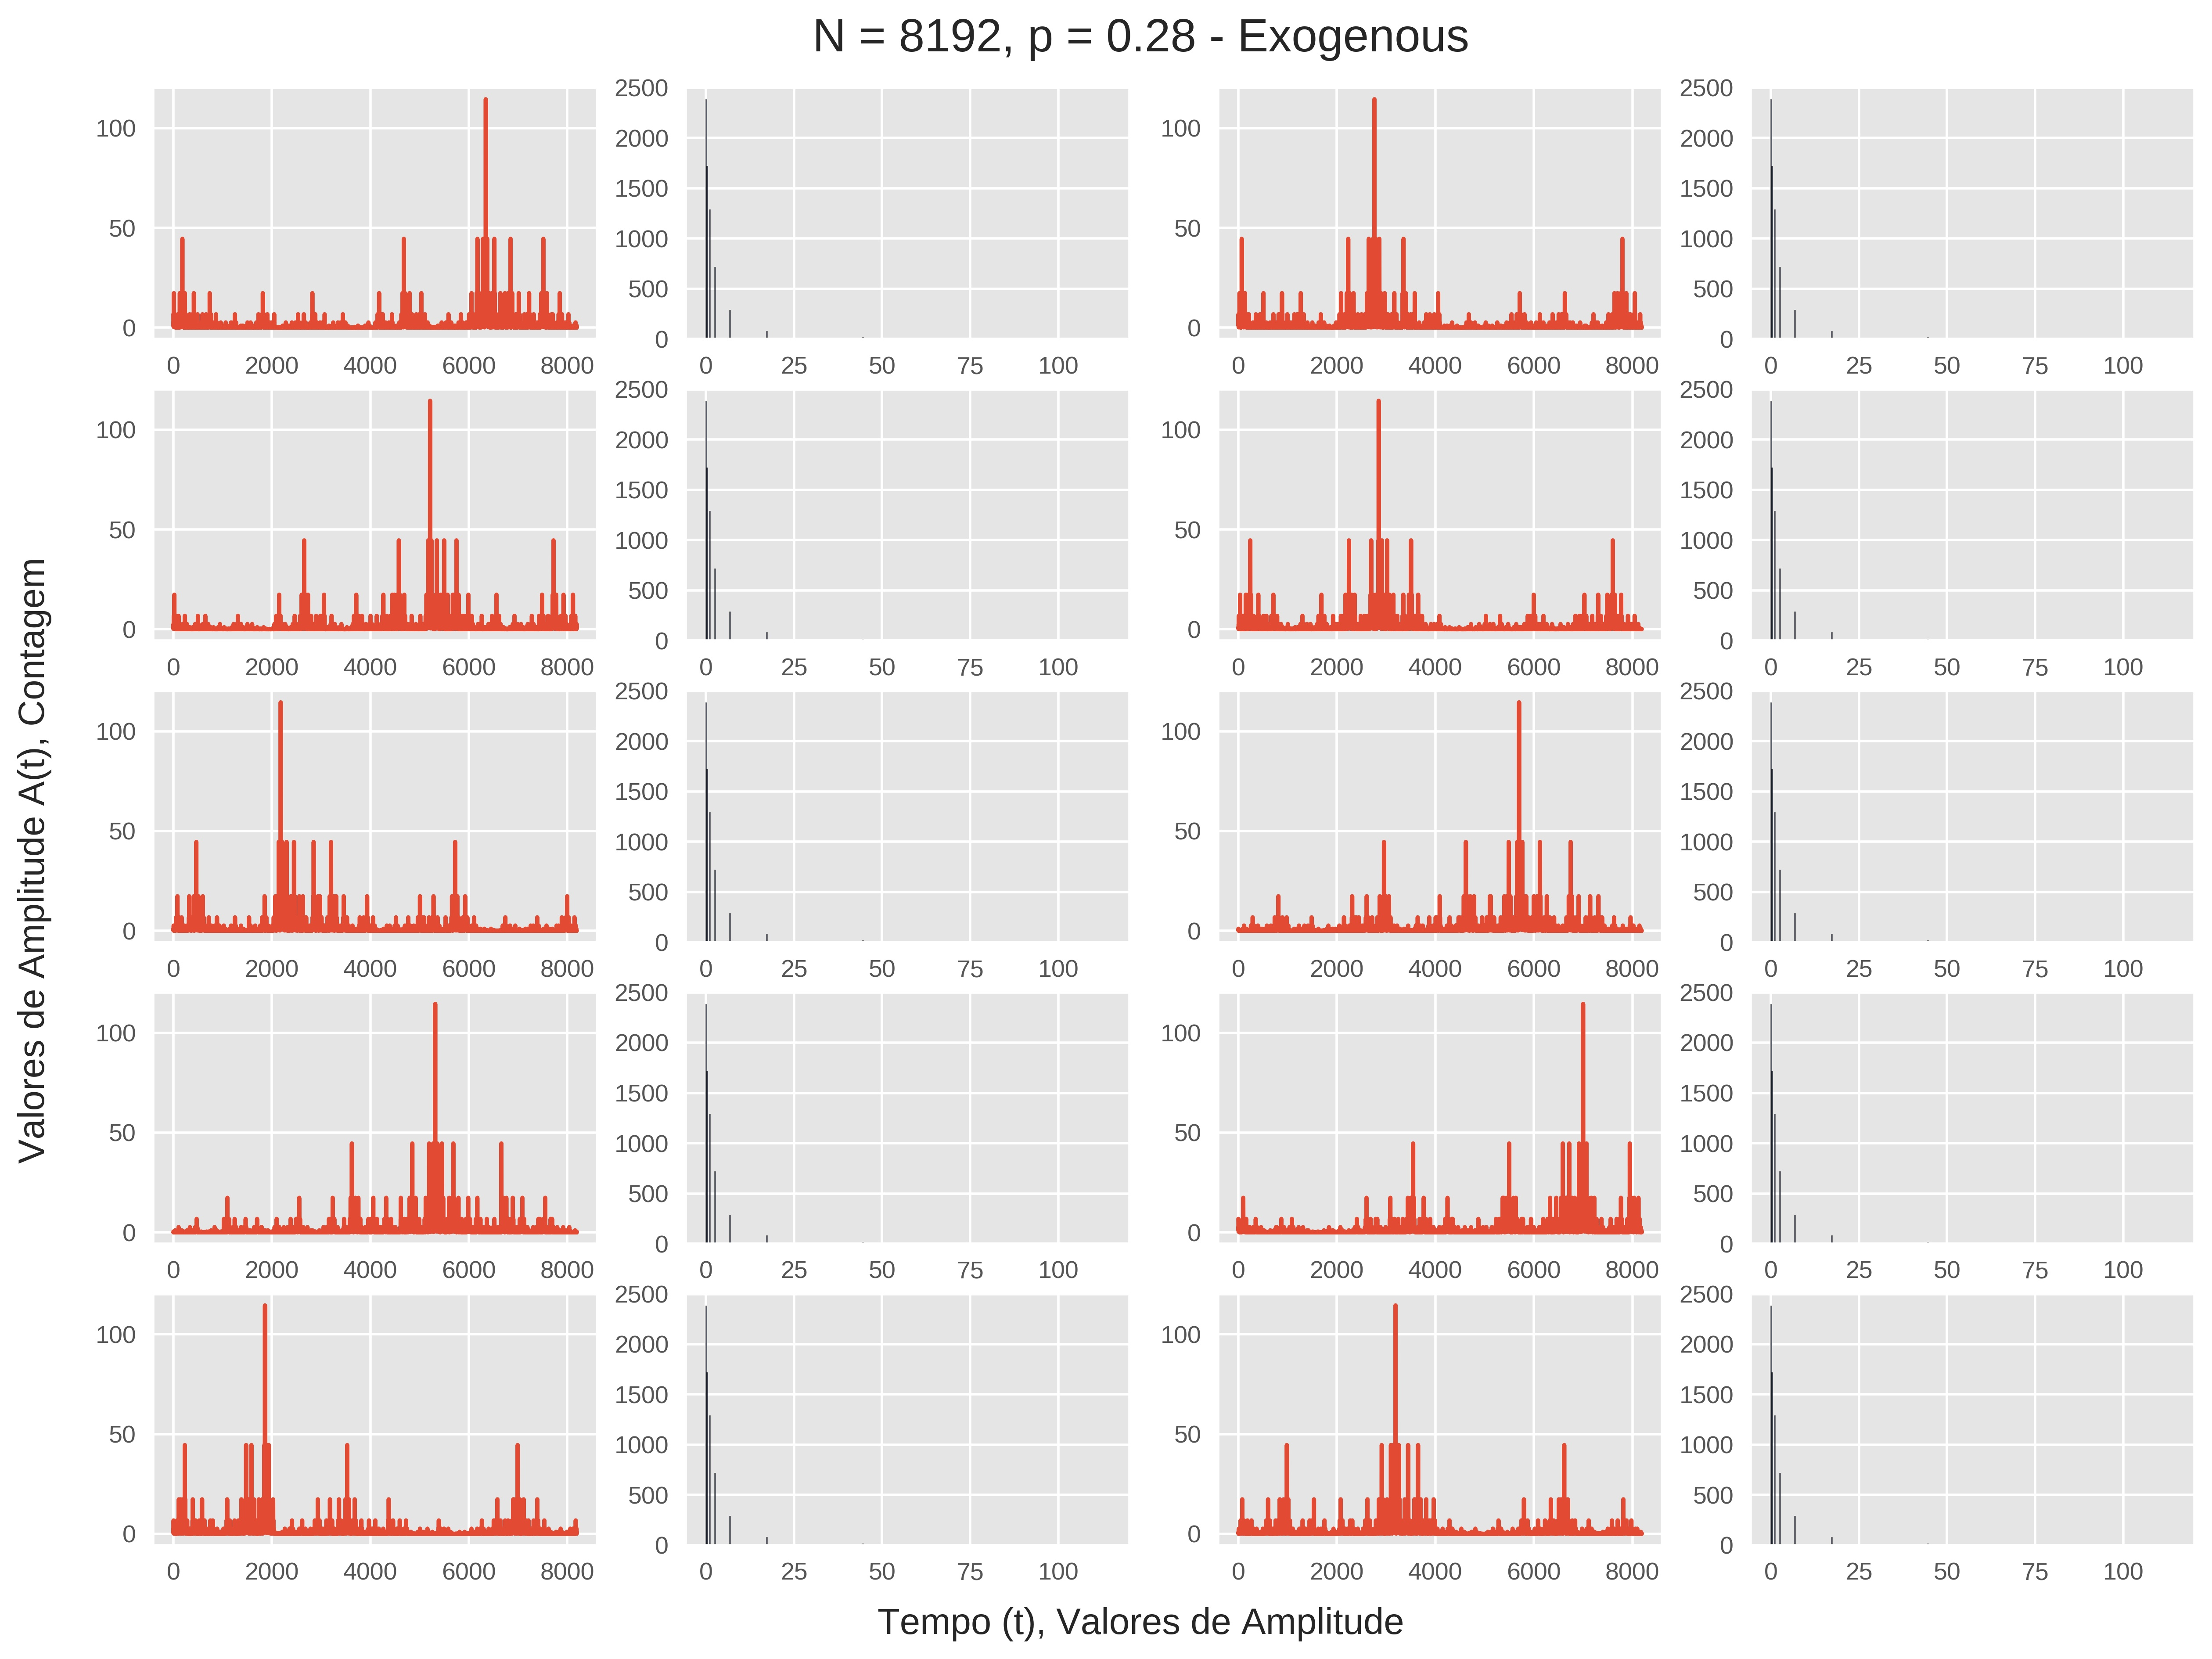
\includegraphics{Figuras/ex3/Exercicio3_p_0.28.jpg}}		
	\end{center}
	\vspace{-2mm}	% acrescentar o espaçamento vertical apropriado entre a borda inferior da figura e a legenda ou a fonte quando não há legenda (o valor pode ser negativo para subir)
	\legenda{Figura 3.1: Plots de 10 sinais da séire exógena ($\beta$ = 0.7) da família pmnoise e seus respectivos histogramas.}	% legenda - para deixar sem legenda usar comando \legenda{} (nunca deve-se comentar o comando \legenda)
	\label{ex3_fig1}
	%\FONTE{}	% fonte consultada (elemento obrigatório, mesmo que seja produção do próprio autor)
\end{figure}

\clearpage

\begin{figure}[ht!]
	%\caption{Série e histogramas.}
	\vspace{0mm}	% acrescentar o espaçamento vertical apropriado entre o título e a borda superior da figura
	\begin{center}
		\resizebox{16cm}{!}{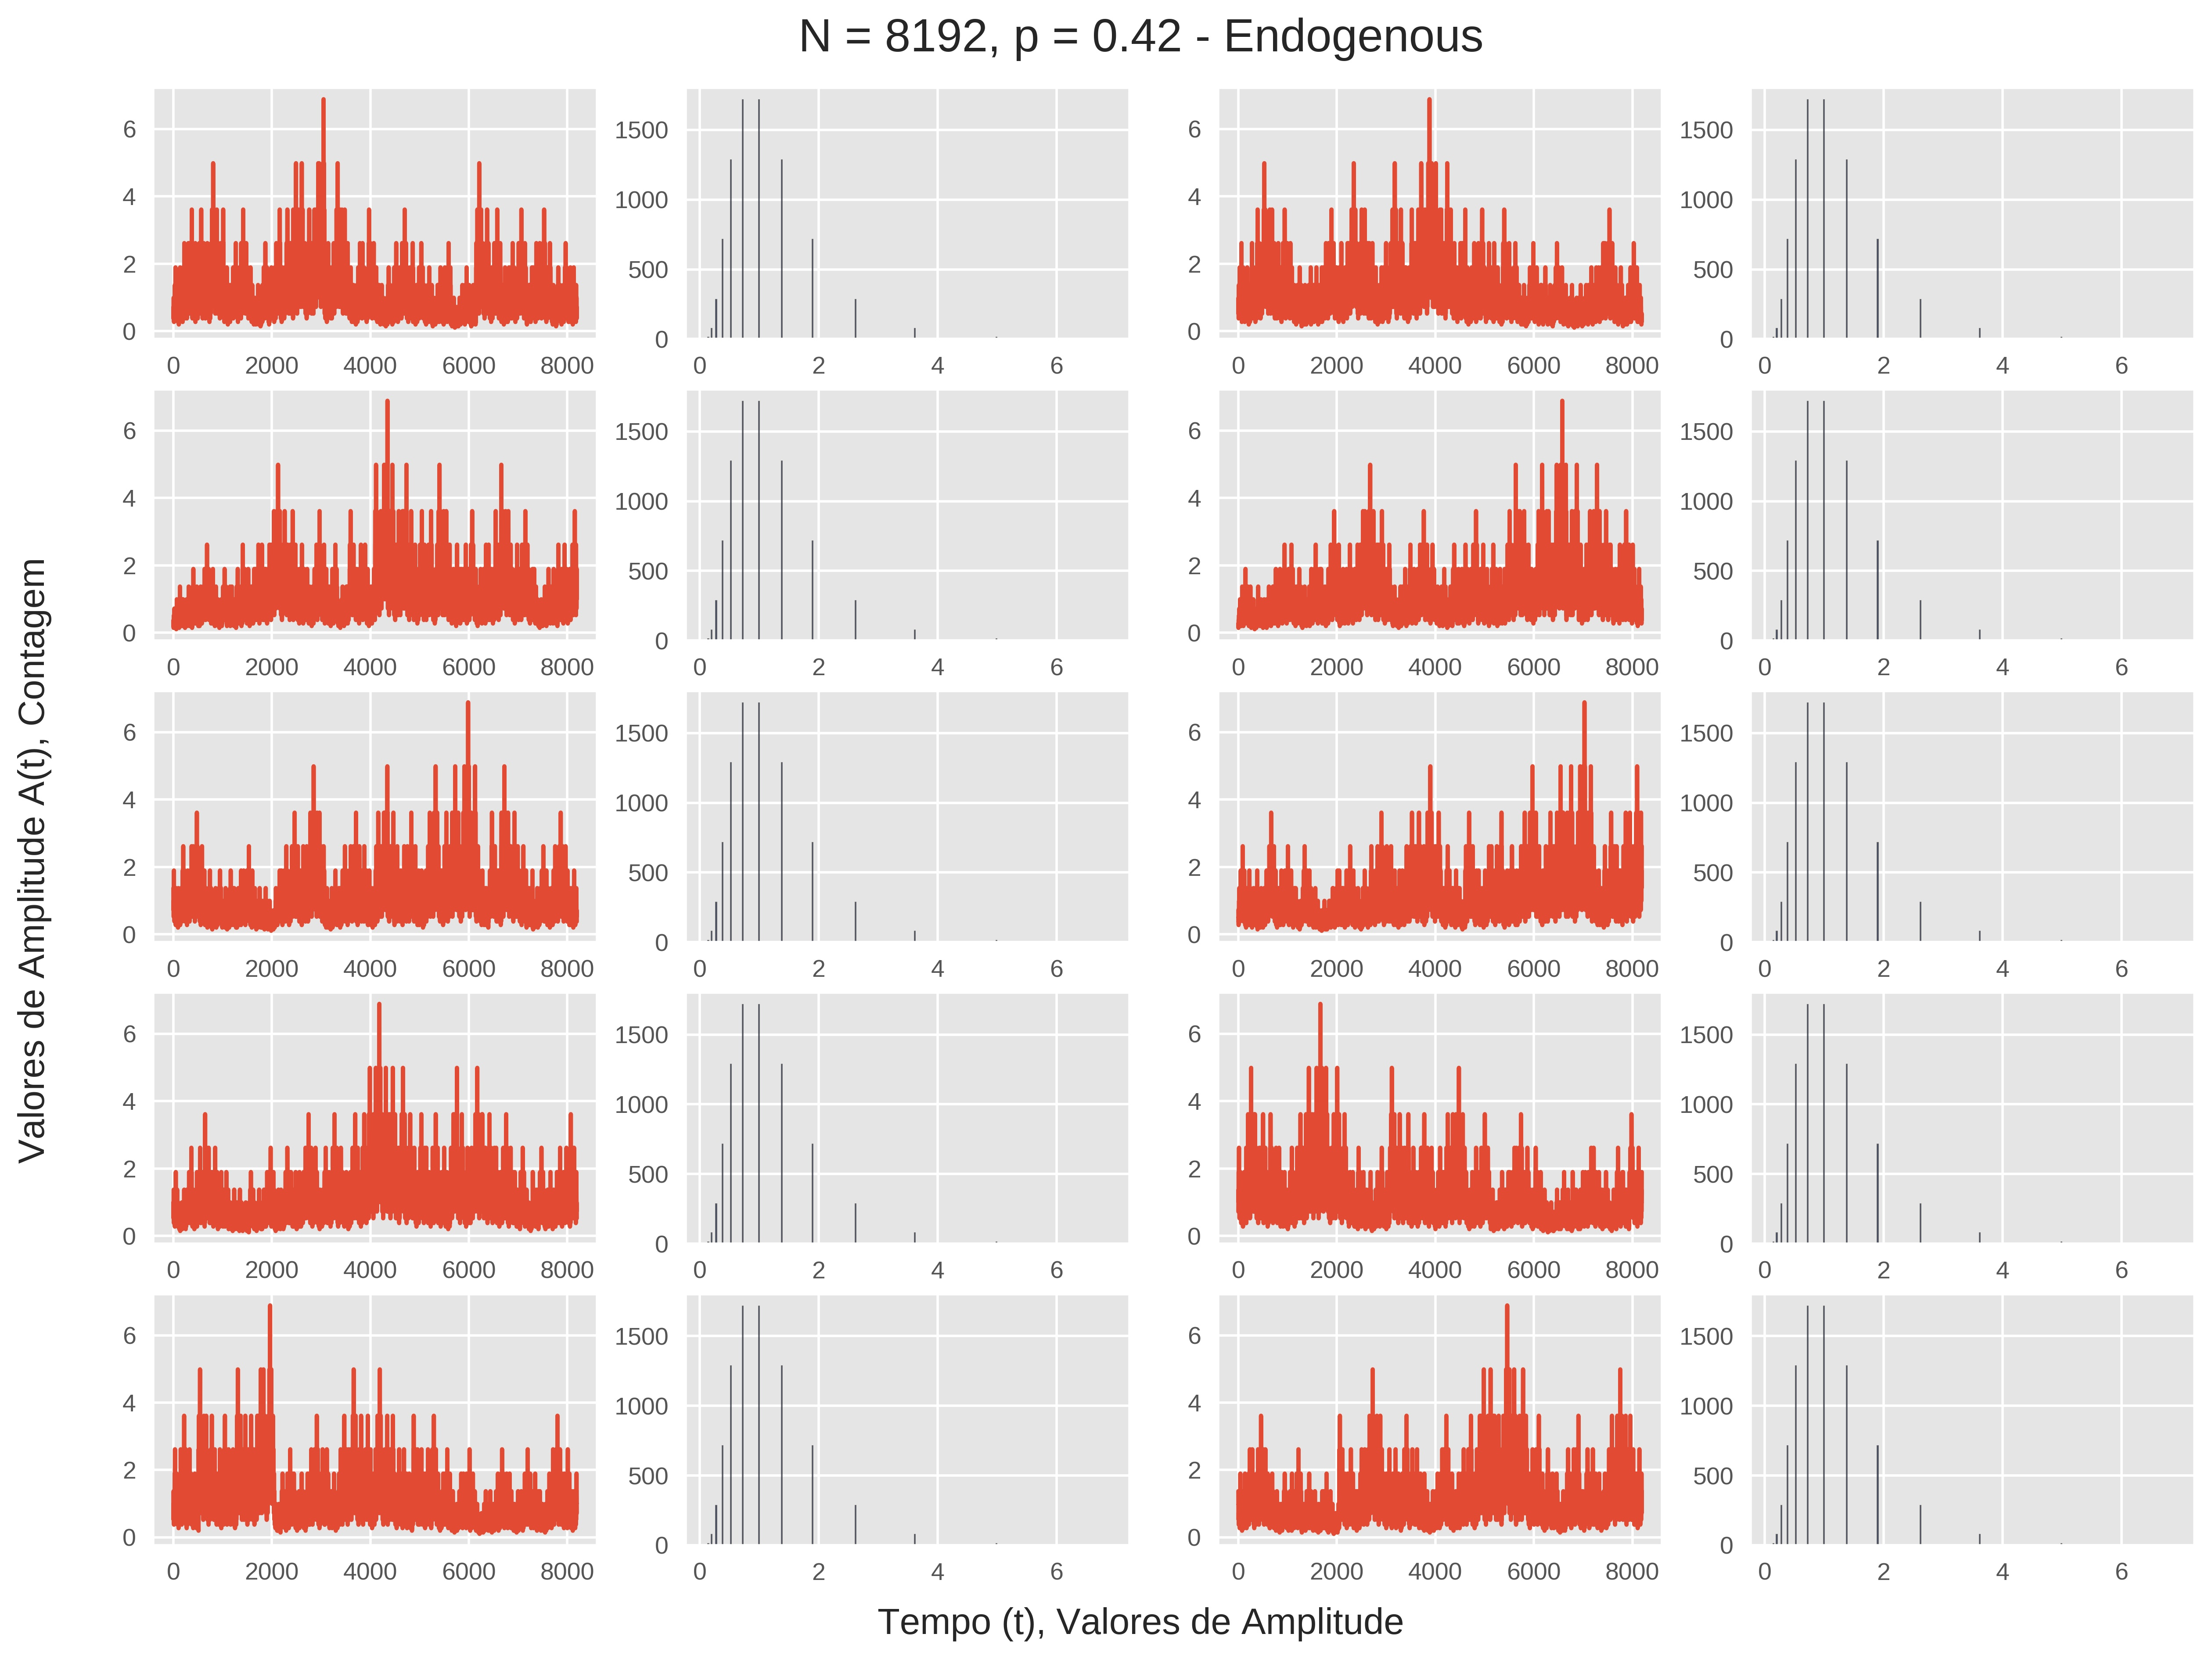
\includegraphics{Figuras/ex3/Exercicio3_p_0.42.jpg}}		
	\end{center}
	\vspace{-2mm}	% acrescentar o espaçamento vertical apropriado entre a borda inferior da figura e a legenda ou a fonte quando não há legenda (o valor pode ser negativo para subir)
	\legenda{Figura 3.2: Plots de 10 sinais da séire endógena ($\beta$ = 0.4) da família pmnoise e seus respectivos histogramas.}	% legenda - para deixar sem legenda usar comando \legenda{} (nunca deve-se comentar o comando \legenda)
	\label{ex3_fig2}
	%\FONTE{}	% fonte consultada (elemento obrigatório, mesmo que seja produção do próprio autor)
\end{figure}

Assim como para as famílias anteriores, a família pmnoise conta com os arquivos \textit{Exercicio3\_momentos.csv},  \textit{Exercicio3\_parametros.csv} e \textit{Exercicio3\_kmeans.csv} em sua pasta, compondo o resultado da análise estatística em conjunto com os demais plots. Abaixo estão os resultados do agrupamento no espaço via kmeans. Fica evidente que há pouca variabilidade de cada sinal no espaço de parâmetros usado, de forma que o agrupamento não permite a caracterização de classes do grupo pmnoise no espaço composto por variância, skewness e kurtosis.

\begin{figure}[ht!]
	%\caption{Série e histogramas.}
	\vspace{0mm}	% acrescentar o espaçamento vertical apropriado entre o título e a borda superior da figura
	\begin{center}
		\resizebox{16cm}{!}{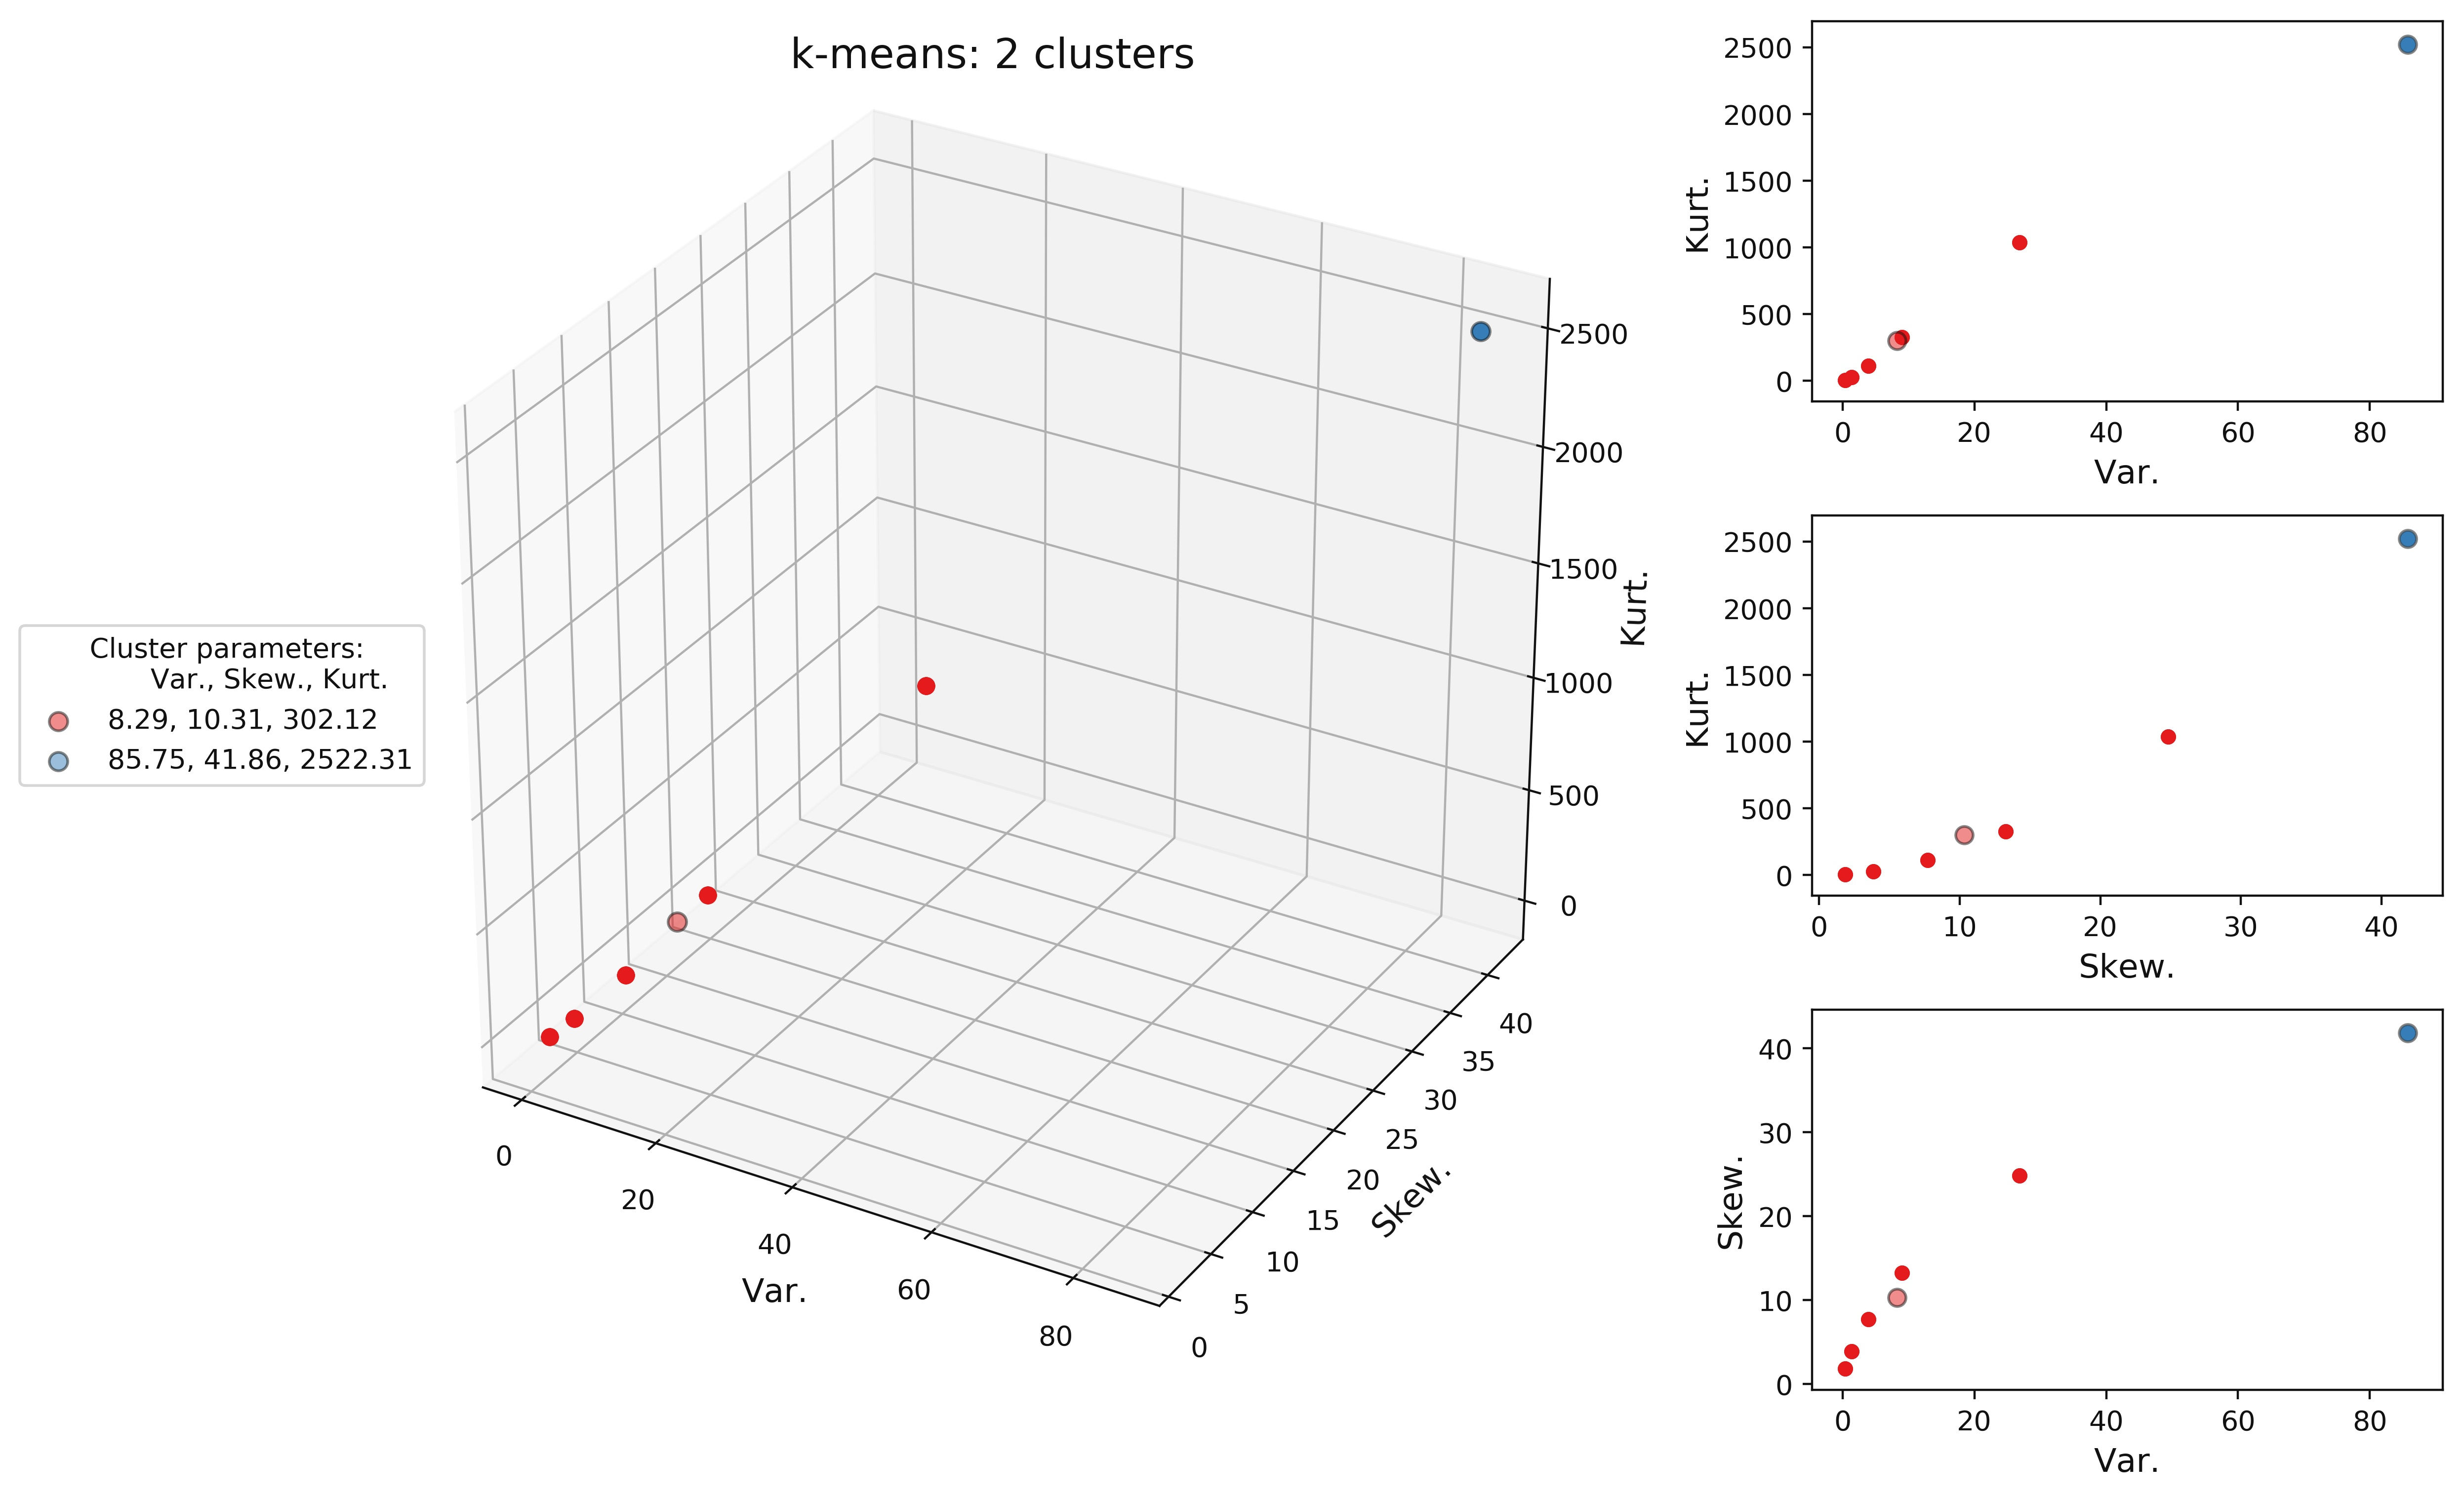
\includegraphics{Figuras/ex3/Exercicio3_cluster_2.jpg}}		
	\end{center}
	\vspace{-2mm}	% acrescentar o espaçamento vertical apropriado entre a borda inferior da figura e a legenda ou a fonte quando não há legenda (o valor pode ser negativo para subir)
	\legenda{Figura 3.3: Técnica kmeans no espaço de parâmetros variância x skewness x kurtosis para todos os sinais da família de sinais pmnoise (endógenos e exógenos). Resultado para número de clusters $n\_c$ = 2.}	% legenda - para deixar sem legenda usar comando \legenda{} (nunca deve-se comentar o comando \legenda)
	\label{ex3_fig3}
	%\FONTE{}	% fonte consultada (elemento obrigatório, mesmo que seja produção do próprio autor)
\end{figure}

\begin{figure}[ht!]
	%\caption{Série e histogramas.}
	\vspace{-3mm}	% acrescentar o espaçamento vertical apropriado entre o título e a borda superior da figura
	\begin{center}
		\resizebox{11cm}{!}{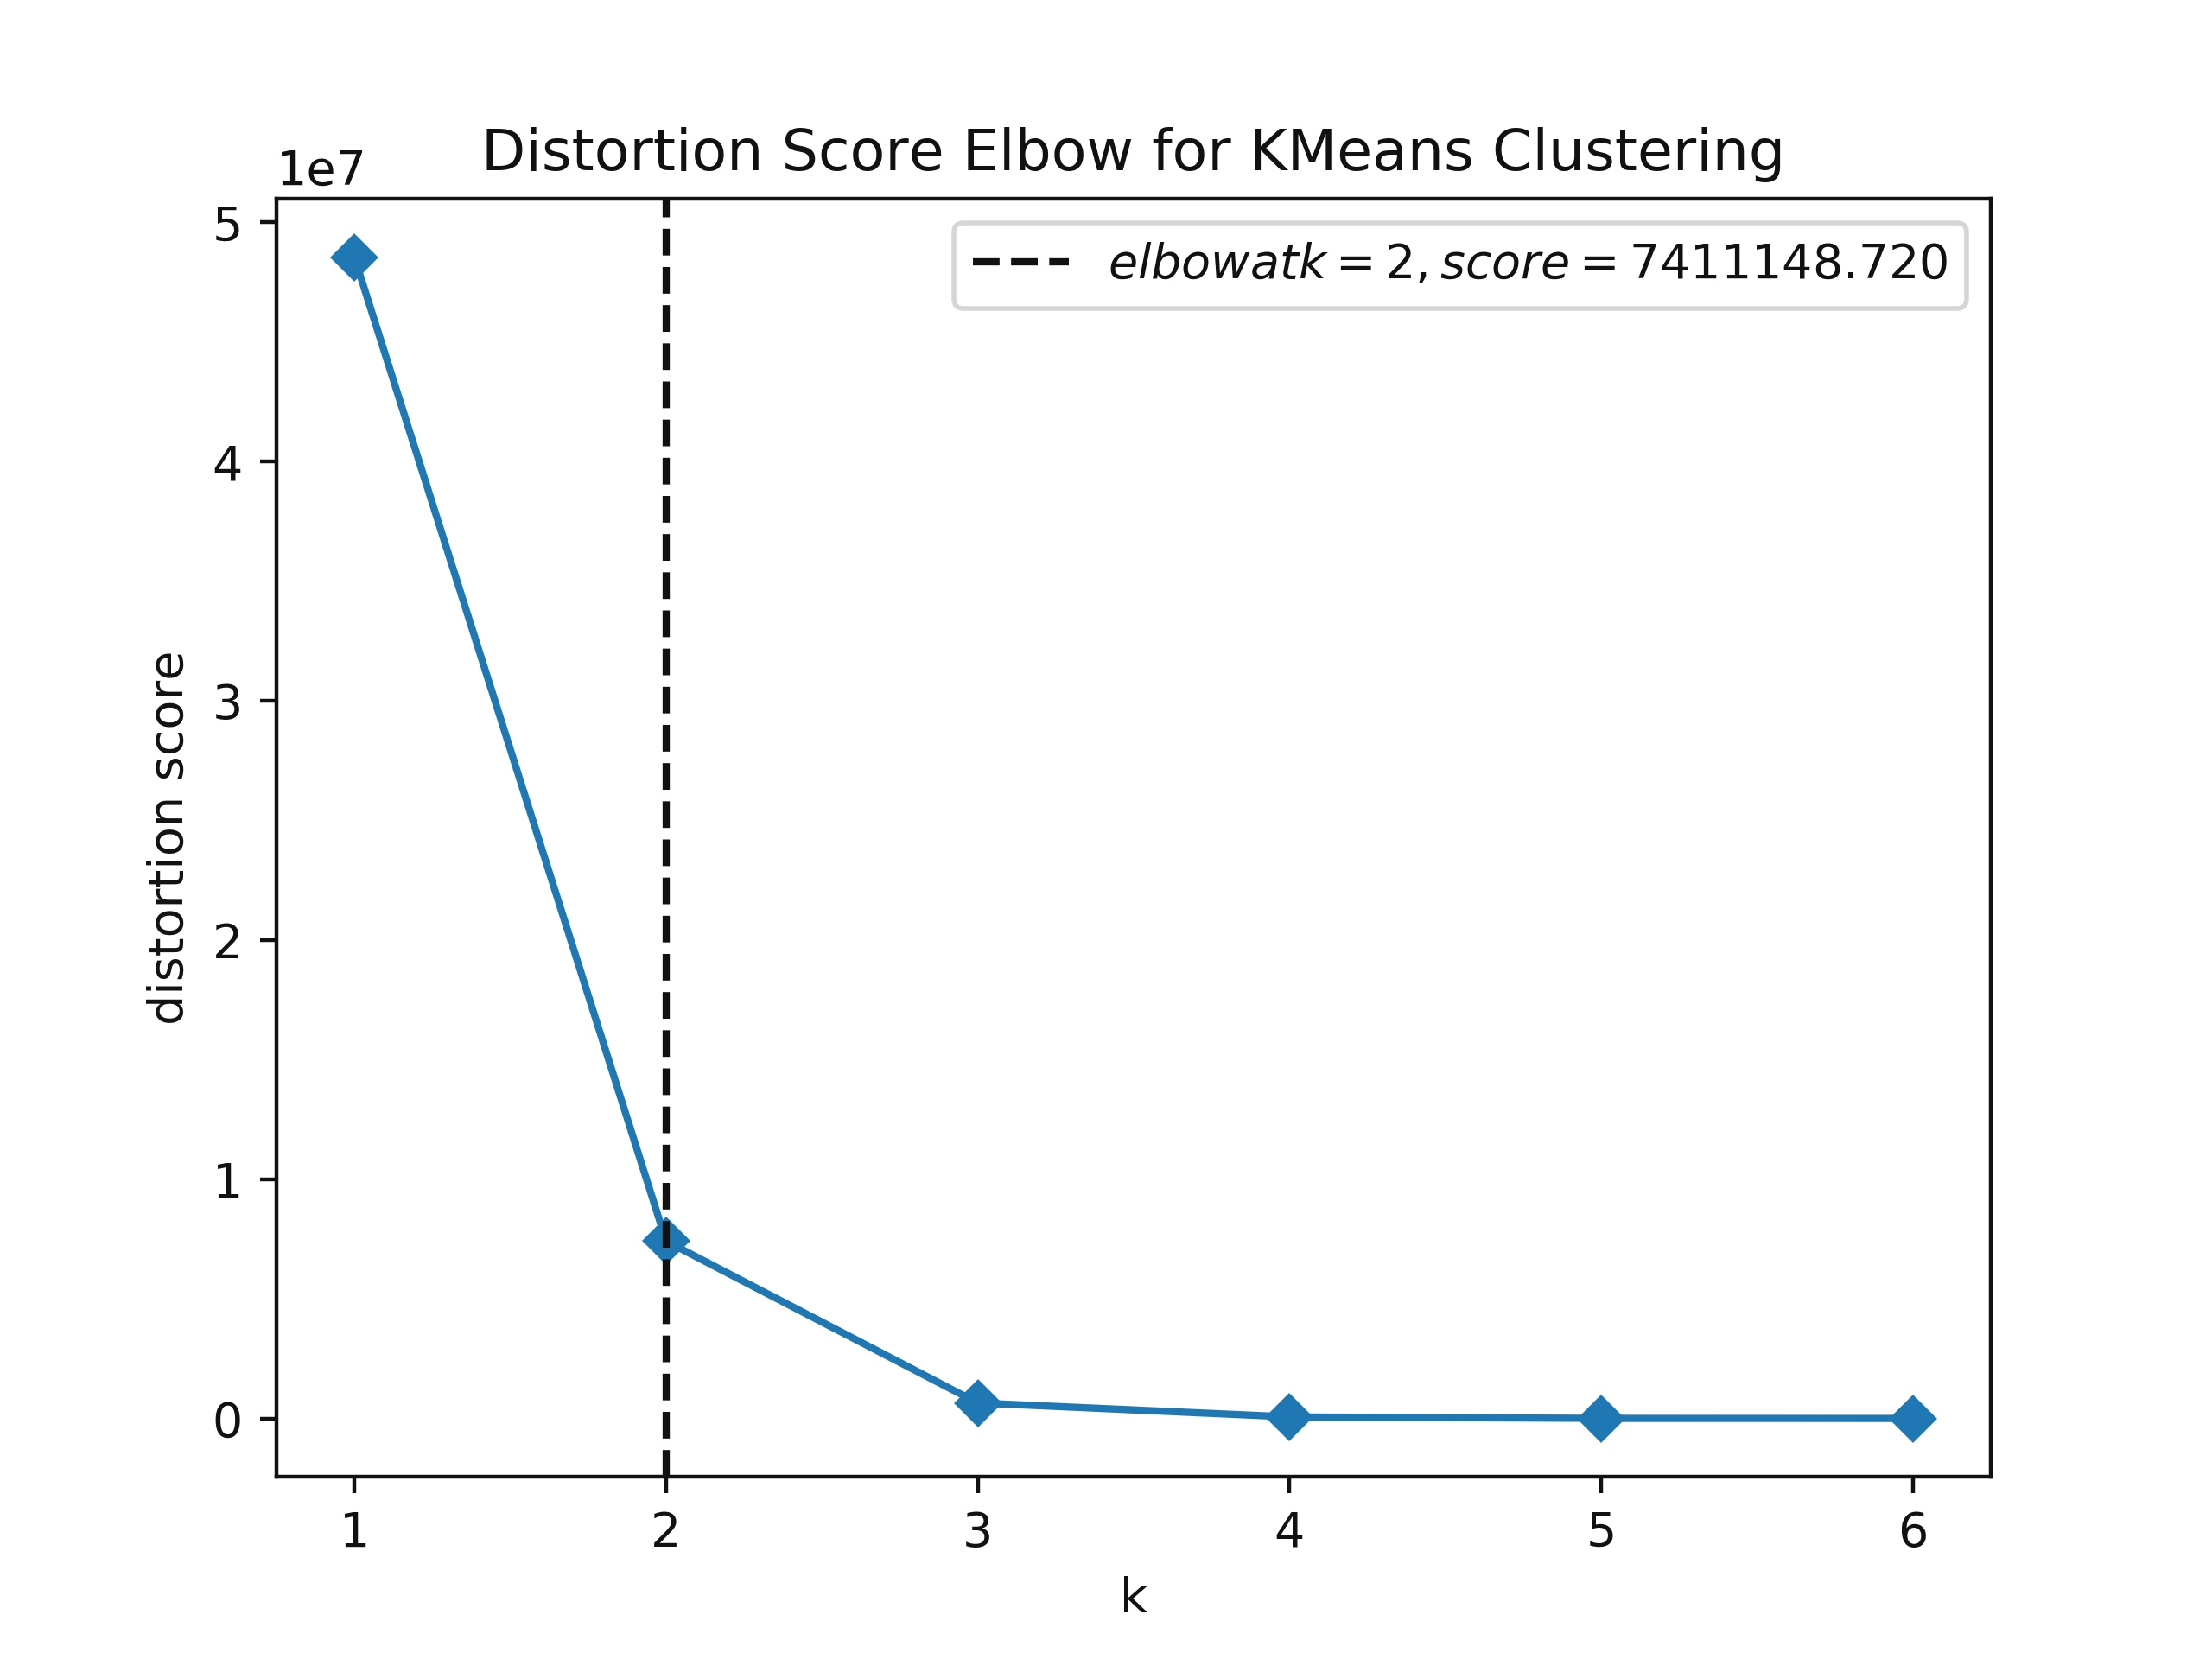
\includegraphics{Figuras/ex3/Exercicio3_elbow_algorithm.jpg}}		
	\end{center}
	\vspace{-3mm}	% acrescentar o espaçamento vertical apropriado entre a borda inferior da figura e a legenda ou a fonte quando não há legenda (o valor pode ser negativo para subir)
	\legenda{Figura 3.4: Resultado do método do cotovelo, mostrando que $n\_c$ = 2 obteve a melhor performance durante o agrupamento da família pmnoise no espaço de parâmetros considerado.}	% legenda - para deixar sem legenda usar comando \legenda{} (nunca deve-se comentar o comando \legenda)
	\label{ex3_fig4}
	%\FONTE{}	% fonte consultada (elemento obrigatório, mesmo que seja produção do próprio autor)
\end{figure}
 %% 3o capítulo

\clearpage
%%%%%%%%%%%%%%%%%%%%%%%%%%%%%%%%%%%%%%%%%%%%%%%%%%%%%%%%%%%%%%%%%%%%%%%%%%%%%%%

\section*{\large Exercício 4 - Espaço de Cullen-Frey e Distribuições de Probabilidades}
\addcontentsline{toc}{chapter}{\protect\numberline{}\large Exercício 4}%

Os resultados deste exercício se encontram na pasta \textbf{Exercise4}. Na pasta \textbf{familia1} estão as análises do grupo noise para $n$ = 8192, e na pasta \textbf{familia2} as análises do grupo colornoise para $n$ = 8192 e $\beta$ = 0.

\subsection*{4.1} 
\addcontentsline{toc}{section}{\protect\numberline{} 4.1}%

A análise desta Seção foi realizada com o script CullenFrey\_R\_Python.py.

\begin{figure}[ht!]
	%\caption{Série e histogramas.}
	\vspace{0mm}	% acrescentar o espaçamento vertical apropriado entre o título e a borda superior da figura
	\begin{center}
		\resizebox{12.5cm}{!}{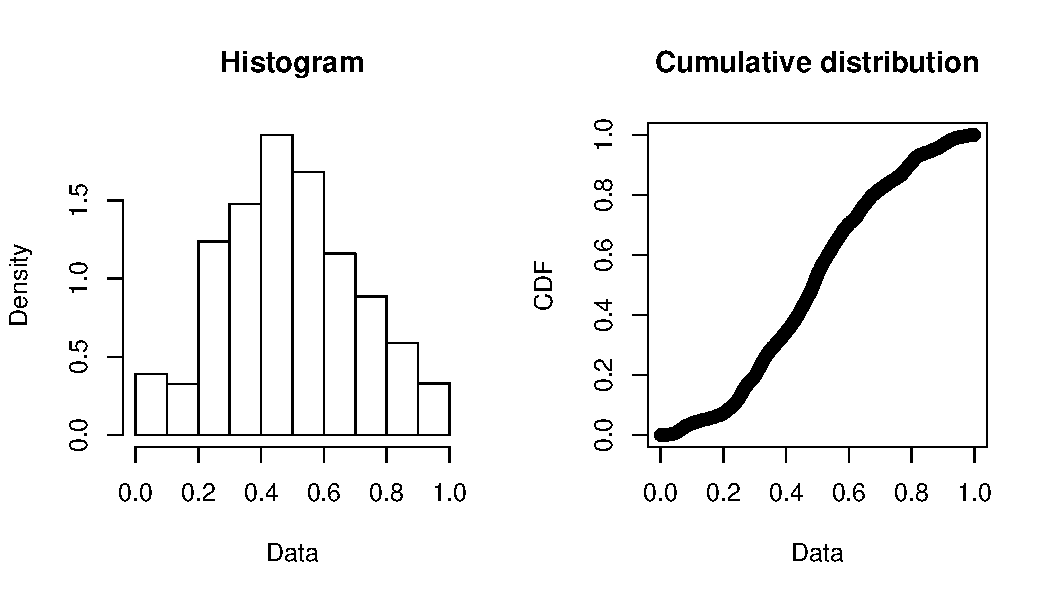
\includegraphics{Figuras/ex4/4_1/Exercicio4_1_fam1_histCDF.pdf}}		
	\end{center}
	\vspace{-2mm}	% acrescentar o espaçamento vertical apropriado entre a borda inferior da figura e a legenda ou a fonte quando não há legenda (o valor pode ser negativo para subir)
	\legenda{Figura 4.1.1: Histograma e CDF para a família 1 (noise) com $n$ = 8192.}	% legenda - para deixar sem legenda usar comando \legenda{} (nunca deve-se comentar o comando \legenda)
	\label{ex4_fig1}
	%\FONTE{}	% fonte consultada (elemento obrigatório, mesmo que seja produção do próprio autor)
\end{figure}

\begin{figure}[ht!]
	%\caption{Série e histogramas.}
	\vspace{0mm}	% acrescentar o espaçamento vertical apropriado entre o título e a borda superior da figura
	\begin{center}
		\resizebox{12.5cm}{!}{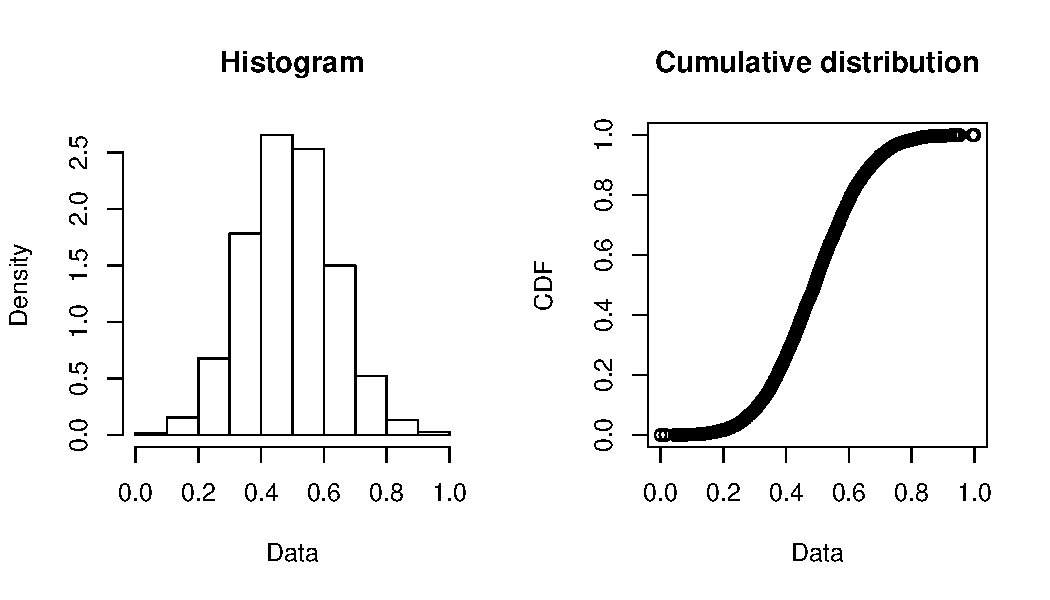
\includegraphics{Figuras/ex4/4_1/Exercicio4_1_fam2_histCDF.pdf}}		
	\end{center}
	\vspace{-2mm}	% acrescentar o espaçamento vertical apropriado entre a borda inferior da figura e a legenda ou a fonte quando não há legenda (o valor pode ser negativo para subir)
	\legenda{Figura 4.1.2: Histograma e CDF para a família 2 (colornoise) com $n$ = 8192 e $\beta$ = 0.}	% legenda - para deixar sem legenda usar comando \legenda{} (nunca deve-se comentar o comando \legenda)
	\label{ex4_fig2}
	%\FONTE{}	% fonte consultada (elemento obrigatório, mesmo que seja produção do próprio autor)
\end{figure}

\begin{figure}[ht!]
	%\caption{Série e histogramas.}
	\vspace{-3mm}	% acrescentar o espaçamento vertical apropriado entre o título e a borda superior da figura
	\begin{center}
		\resizebox{10.cm}{!}{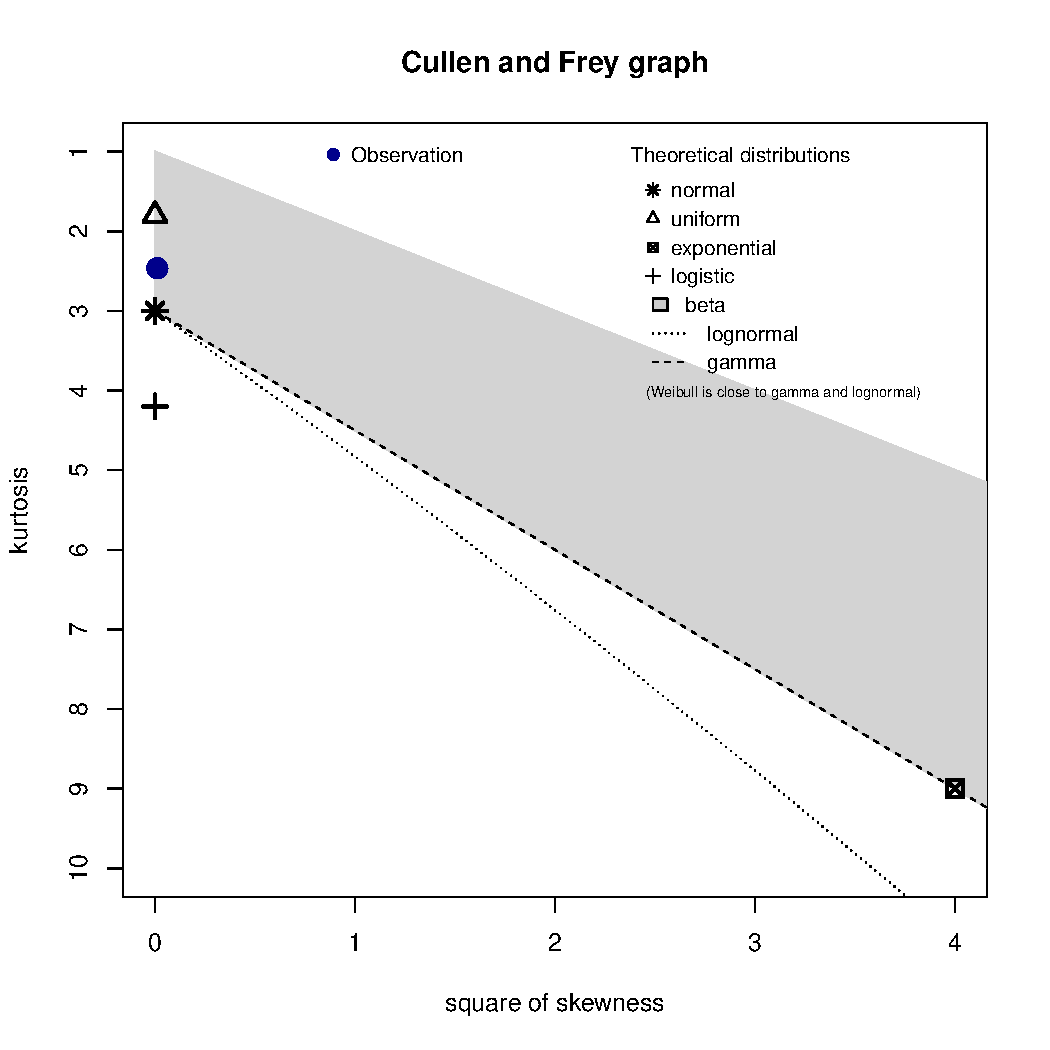
\includegraphics{Figuras/ex4/4_1/Exercicio4_1_fam1_CullenFrey.pdf}}		
	\end{center}
	\vspace{-3mm}	% acrescentar o espaçamento vertical apropriado entre a borda inferior da figura e a legenda ou a fonte quando não há legenda (o valor pode ser negativo para subir)
	\legenda{Figura 4.1.3: Resultado da análise Cullen and Frey para a família 1 (noise).}	% legenda - para deixar sem legenda usar comando \legenda{} (nunca deve-se comentar o comando \legenda)
	\label{ex4_fig3}
	%\FONTE{}	% fonte consultada (elemento obrigatório, mesmo que seja produção do próprio autor)
\end{figure}

\begin{figure}[ht!]
	%\caption{Série e histogramas.}
	\vspace{-3mm}	% acrescentar o espaçamento vertical apropriado entre o título e a borda superior da figura
	\begin{center}
		\resizebox{10.cm}{!}{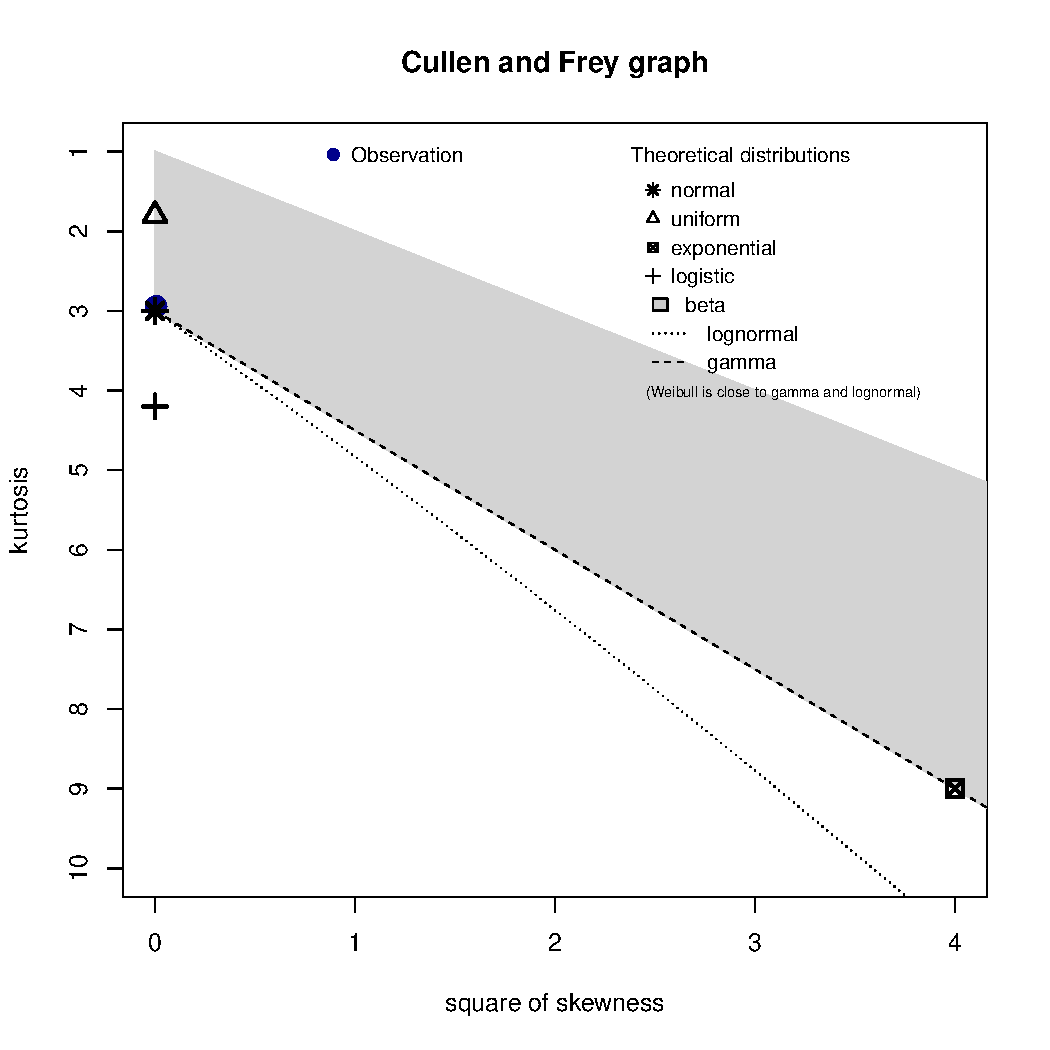
\includegraphics{Figuras/ex4/4_1/Exercicio4_1_fam2_CullenFrey.pdf}}		
	\end{center}
	\vspace{-3mm}	% acrescentar o espaçamento vertical apropriado entre a borda inferior da figura e a legenda ou a fonte quando não há legenda (o valor pode ser negativo para subir)
	\legenda{Figura 4.1.4: Resultado da análise Cullen and Frey para a família 2 (pmnoise).}	% legenda - para deixar sem legenda usar comando \legenda{} (nunca deve-se comentar o comando \legenda)
	\label{ex4_fig4}
	%\FONTE{}	% fonte consultada (elemento obrigatório, mesmo que seja produção do próprio autor)
\end{figure}

%%%%%%%%%%%%%%%%%%%%%%%%%%%%%%%%%%%%%%%%%%% 4.2 %%%%%%%%%%%%%%%%%%%%%%%%%%%%%%%%%%%%%%%%%%%%%%%%
\clearpage
\subsection*{4.2}
\addcontentsline{toc}{section}{\protect\numberline{} 4.2}%

Todos os resultados desta Seção forma gerados com os scripts Distribution\_Fitter\_Python.py e Distribution\_Fitter\_R.py.

%%%%%%%%%%%%%%%%% familia 1 %%%%%%%%%%%%%%%%%%%%%

\subsubsection*{Primeira família}

\begin{figure}[ht!]
	%\caption{Série e histogramas.}
	\vspace{0mm}	% acrescentar o espaçamento vertical apropriado entre o título e a borda superior da figura
	\begin{center}
		\resizebox{13cm}{!}{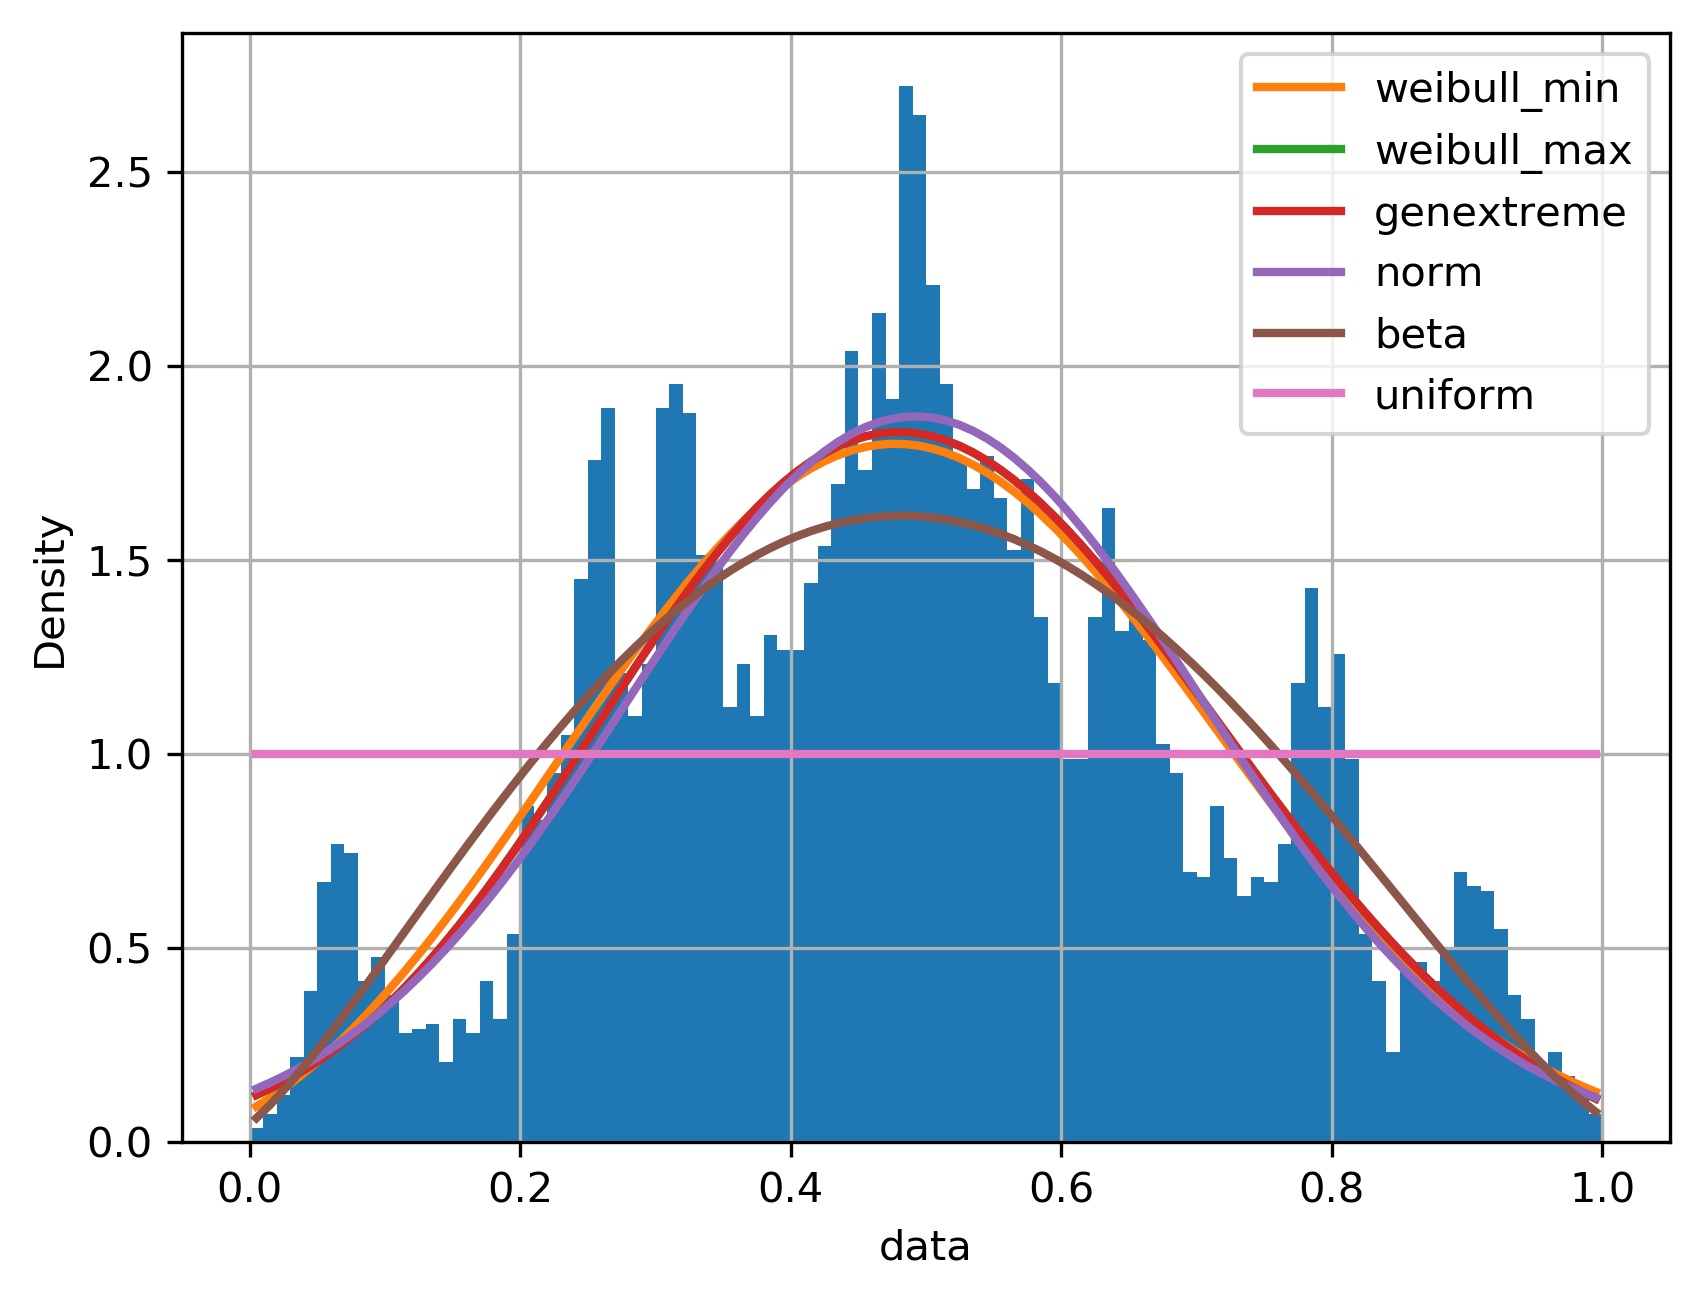
\includegraphics{Figuras/ex4/4_2/Exercicio4_2_fam1_Python_fits.jpg}}		
	\end{center}
	\vspace{-2mm}	% acrescentar o espaçamento vertical apropriado entre a borda inferior da figura e a legenda ou a fonte quando não há legenda (o valor pode ser negativo para subir)
	\legenda{Figura 4.2.1: Resultado do ajuste de 6 distribuições diferentes, incluindo GEV, na família noise. Foi utilizado o script Distribution\_Fitter\_Python.py para este plot.}	% legenda - para deixar sem legenda usar comando \legenda{} (nunca deve-se comentar o comando \legenda)
	\label{ex4_fig8}
	%\FONTE{}	% fonte consultada (elemento obrigatório, mesmo que seja produção do próprio autor)
\end{figure}

Abaixo o resultado do benchmark gerado automaticamente pelo script Distribution\_Fitter\_Python.py, presente no arquivo \textit{Exercicio4\_2\_fam1\_Python\_fits.txt}, que permite avaliar a performance de cada distribuição no ajuste empregado. Observa-se que a \texttt{weibull} foi a distribuição com menor erro.

\begin{figure}[ht!]
	%\caption{Série e histogramas.}
	\vspace{0mm}	% acrescentar o espaçamento vertical apropriado entre o título e a borda superior da figura
	%\begin{center}
		\resizebox{12cm}{!}{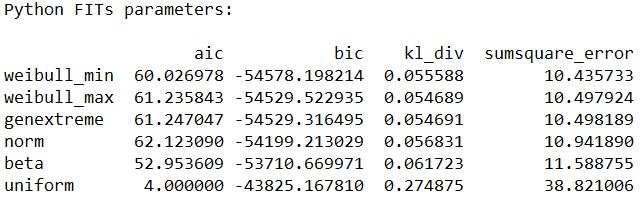
\includegraphics{Figuras/ex4/4_2/Exercicio4_2_fam1_Python_fits_params.jpg}}		
	%\end{center}
	\vspace{-2mm}	% acrescentar o espaçamento vertical apropriado entre a borda inferior da figura e a legenda ou a fonte quando não há legenda (o valor pode ser negativo para subir)
	%\legenda{Figura 4.2.4:.}	% legenda - para deixar sem legenda usar comando \legenda{} (nunca deve-se comentar o comando \legenda)
	%\label{ex4_fig8}
	%\FONTE{}	% fonte consultada (elemento obrigatório, mesmo que seja produção do próprio autor)
\end{figure}

\begin{figure}[ht!]
	%\caption{Série e histogramas.}
	\vspace{-3mm}	% acrescentar o espaçamento vertical apropriado entre o título e a borda superior da figura
	\begin{center}
		\resizebox{12cm}{!}{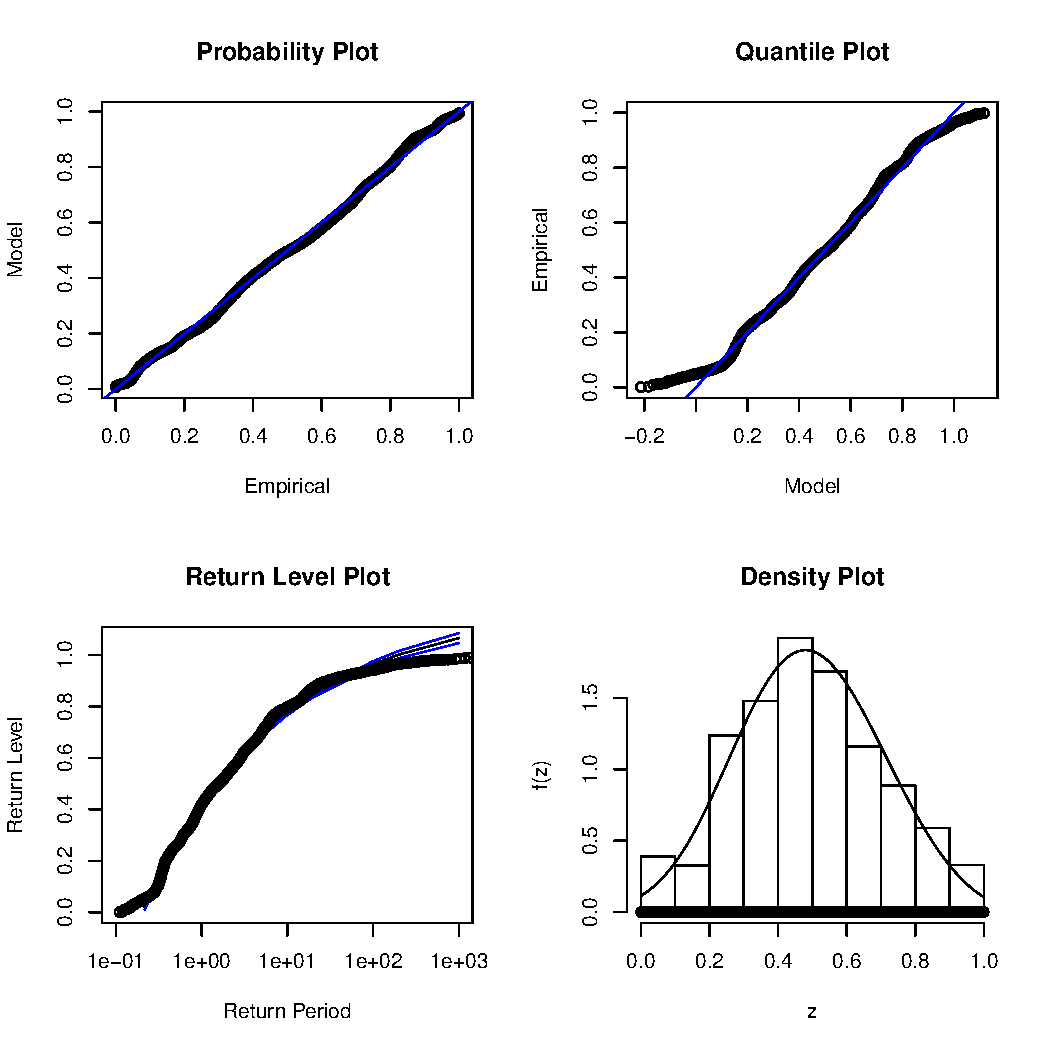
\includegraphics{Figuras/ex4/4_2/Exercicio4_2_fam1_GEV.pdf}}		
	\end{center}
	\vspace{-3mm}	% acrescentar o espaçamento vertical apropriado entre a borda inferior da figura e a legenda ou a fonte quando não há legenda (o valor pode ser negativo para subir)
	\legenda{Figura 4.2.2: Resultado do ajuste da GEV com o script Distribution\_Fitter\_R.py. Um ajuste das mesmas distribuições da Figura 4.2.1 foi gerado, mas essa figura ilustra apenas a performance da GEV com o script com ambiente R em Python, que inclui plots dos quantis teóricos vs os empíricos, e das probabilidades teóricas vs as empíricas, além da curva da GEV sobre o histograma da série.}	% legenda - para deixar sem legenda usar comando \legenda{} (nunca deve-se comentar o comando \legenda)
	\label{ex4_fig6}
	%\FONTE{}	% fonte consultada (elemento obrigatório, mesmo que seja produção do próprio autor)
\end{figure}
%que indica a convergência do ajuste da GEV e 
Abaixo o resultado do benchmark gerado automaticamente pelo script Distribution\_Fitter\_R.py para o ajuste de uma GEV, presente no arquivo \textit{Exercicio4\_2\_fam1\_GEV\_params.txt}, com o resultado dos parâmetros da GEV via \texttt{MLE} (Maximum Likelihood Estimation) e seus respectivos erros.  

\begin{figure}[ht!]
	%\caption{Série e histogramas.}
	\vspace{0mm}	% acrescentar o espaçamento vertical apropriado entre o título e a borda superior da figura
	%\begin{center}
		\resizebox{13.5cm}{!}{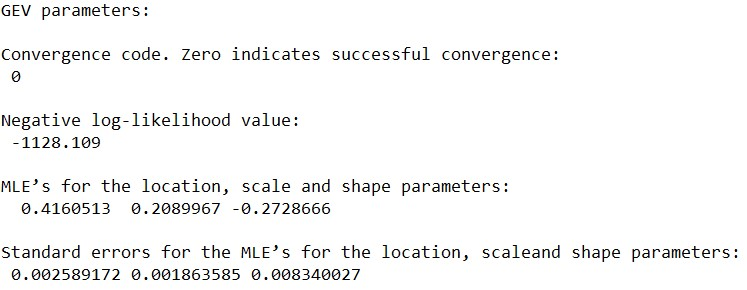
\includegraphics{Figuras/ex4/4_2/Exercicio4_2_fam1_GEV_params.jpg}}		
	%\end{center}
	\vspace{-2mm}	% acrescentar o espaçamento vertical apropriado entre a borda inferior da figura e a legenda ou a fonte quando não há legenda (o valor pode ser negativo para subir)
	%\legenda{Figura 4.2.3:.}	% legenda - para deixar sem legenda usar comando \legenda{} (nunca deve-se comentar o comando \legenda)
	\label{ex4_fig7}
	%\FONTE{}	% fonte consultada (elemento obrigatório, mesmo que seja produção do próprio autor)
\end{figure}

%%%%%%%%%%%%%%%%%%%%%%% familia 2 %%%%%%%%%%%%%%%%%%%%%%%%
\clearpage
\subsubsection*{Segunda família}

\begin{figure}[ht!]
	%\caption{Série e histogramas.}
	\vspace{0mm}	% acrescentar o espaçamento vertical apropriado entre o título e a borda superior da figura
	\begin{center}
		\resizebox{12cm}{!}{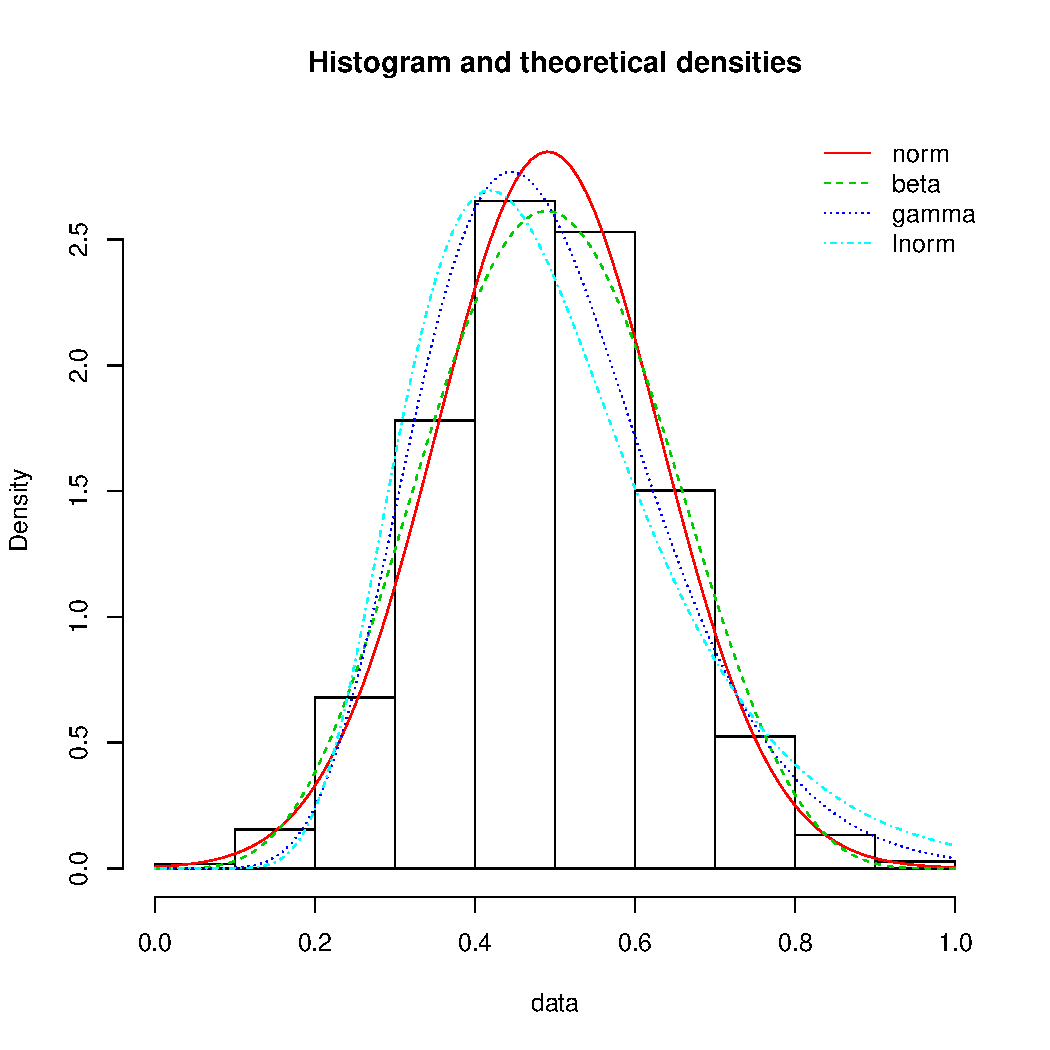
\includegraphics{Figuras/ex4/4_2/Exercicio4_2_fam2_fitComp.pdf}}		
	\end{center}
	\vspace{-2mm}	% acrescentar o espaçamento vertical apropriado entre a borda inferior da figura e a legenda ou a fonte quando não há legenda (o valor pode ser negativo para subir)
	\legenda{Figura 4.2.3: Resultado do ajuste de 4 distribuições diferentes na família pmnoise. Foi utilizado o script Distribution\_Fitter\_R.py para este plot. Não foi ajustada uma GEV para esta família.}	% legenda - para deixar sem legenda usar comando \legenda{} (nunca deve-se comentar o comando \legenda)
	\label{ex4_fig9}
	%\FONTE{}	% fonte consultada (elemento obrigatório, mesmo que seja produção do próprio autor)
\end{figure}

Abaixo o resultado do benchmark gerado automaticamente pelo script Distribution\_Fitter\_R.py, presente no arquivo \textit{Exercicio4\_2\_fam1\_gof.txt}, com o resultado dos ajustes através do método \texttt{mle} (maximum likelihood estimation), que é o padrão do código. Observa-se que a distribuição \texttt{normal} foi a de melhor performance.

\begin{figure}[ht!]
	%\caption{Série e histogramas.}
	\vspace{0mm}	% acrescentar o espaçamento vertical apropriado entre o título e a borda superior da figura
	%\begin{center}
		\resizebox{14cm}{!}{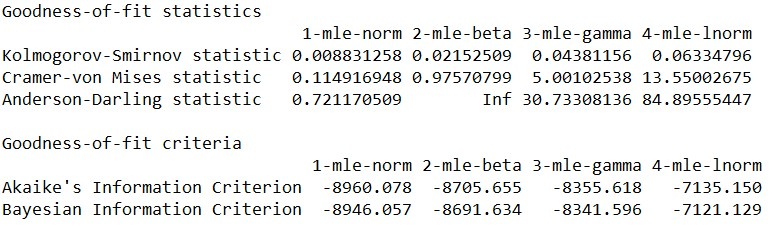
\includegraphics{Figuras/ex4/4_2/Exercicio4_2_fam2_gof.jpg}}		
	%\end{center}
	\vspace{-2mm}	% acrescentar o espaçamento vertical apropriado entre a borda inferior da figura e a legenda ou a fonte quando não há legenda (o valor pode ser negativo para subir)
	%\legenda{Figura 4.2.6:.}	% legenda - para deixar sem legenda usar comando \legenda{} (nunca deve-se comentar o comando \legenda)
	\label{ex4_fig10}
	%\FONTE{}	% fonte consultada (elemento obrigatório, mesmo que seja produção do próprio autor)
\end{figure}

 %% 4o capítulo

\clearpage
%%%%%%%%%%%%%%%%%%%%%%%%%%%%%%%%%%%%%%%%%%%%%%%%%%%%%%%%%%%%%%%%%%%%%%%%%%%%%%%

\section*{\large Exercício 5 - Processos Estocásticos Canônicos: Caos Determinístico e Turbulência}
\addcontentsline{toc}{chapter}{\protect\numberline{}\large Exercício 5}%

Os resultados deste exercício se encontram na pasta \textbf{Exercise4}, junto com todas as análises da família chaosnoise, separadas entre a pasta \textbf{Logístico} e \textbf{Henon}.

\subsection*{5.1}
\addcontentsline{toc}{section}{\protect\numberline{} 5.1}%

\subsubsection*{Logístico}
Para o mapeamento Logístico, os valores de $\rho$ escolhidos foram 3.81, 3.905 e 4. 

\begin{figure}[ht!]
	%\caption{Série e histogramas.}
	\vspace{0mm}	% acrescentar o espaçamento vertical apropriado entre o título e a borda superior da figura
	\begin{center}
		\resizebox{16cm}{!}{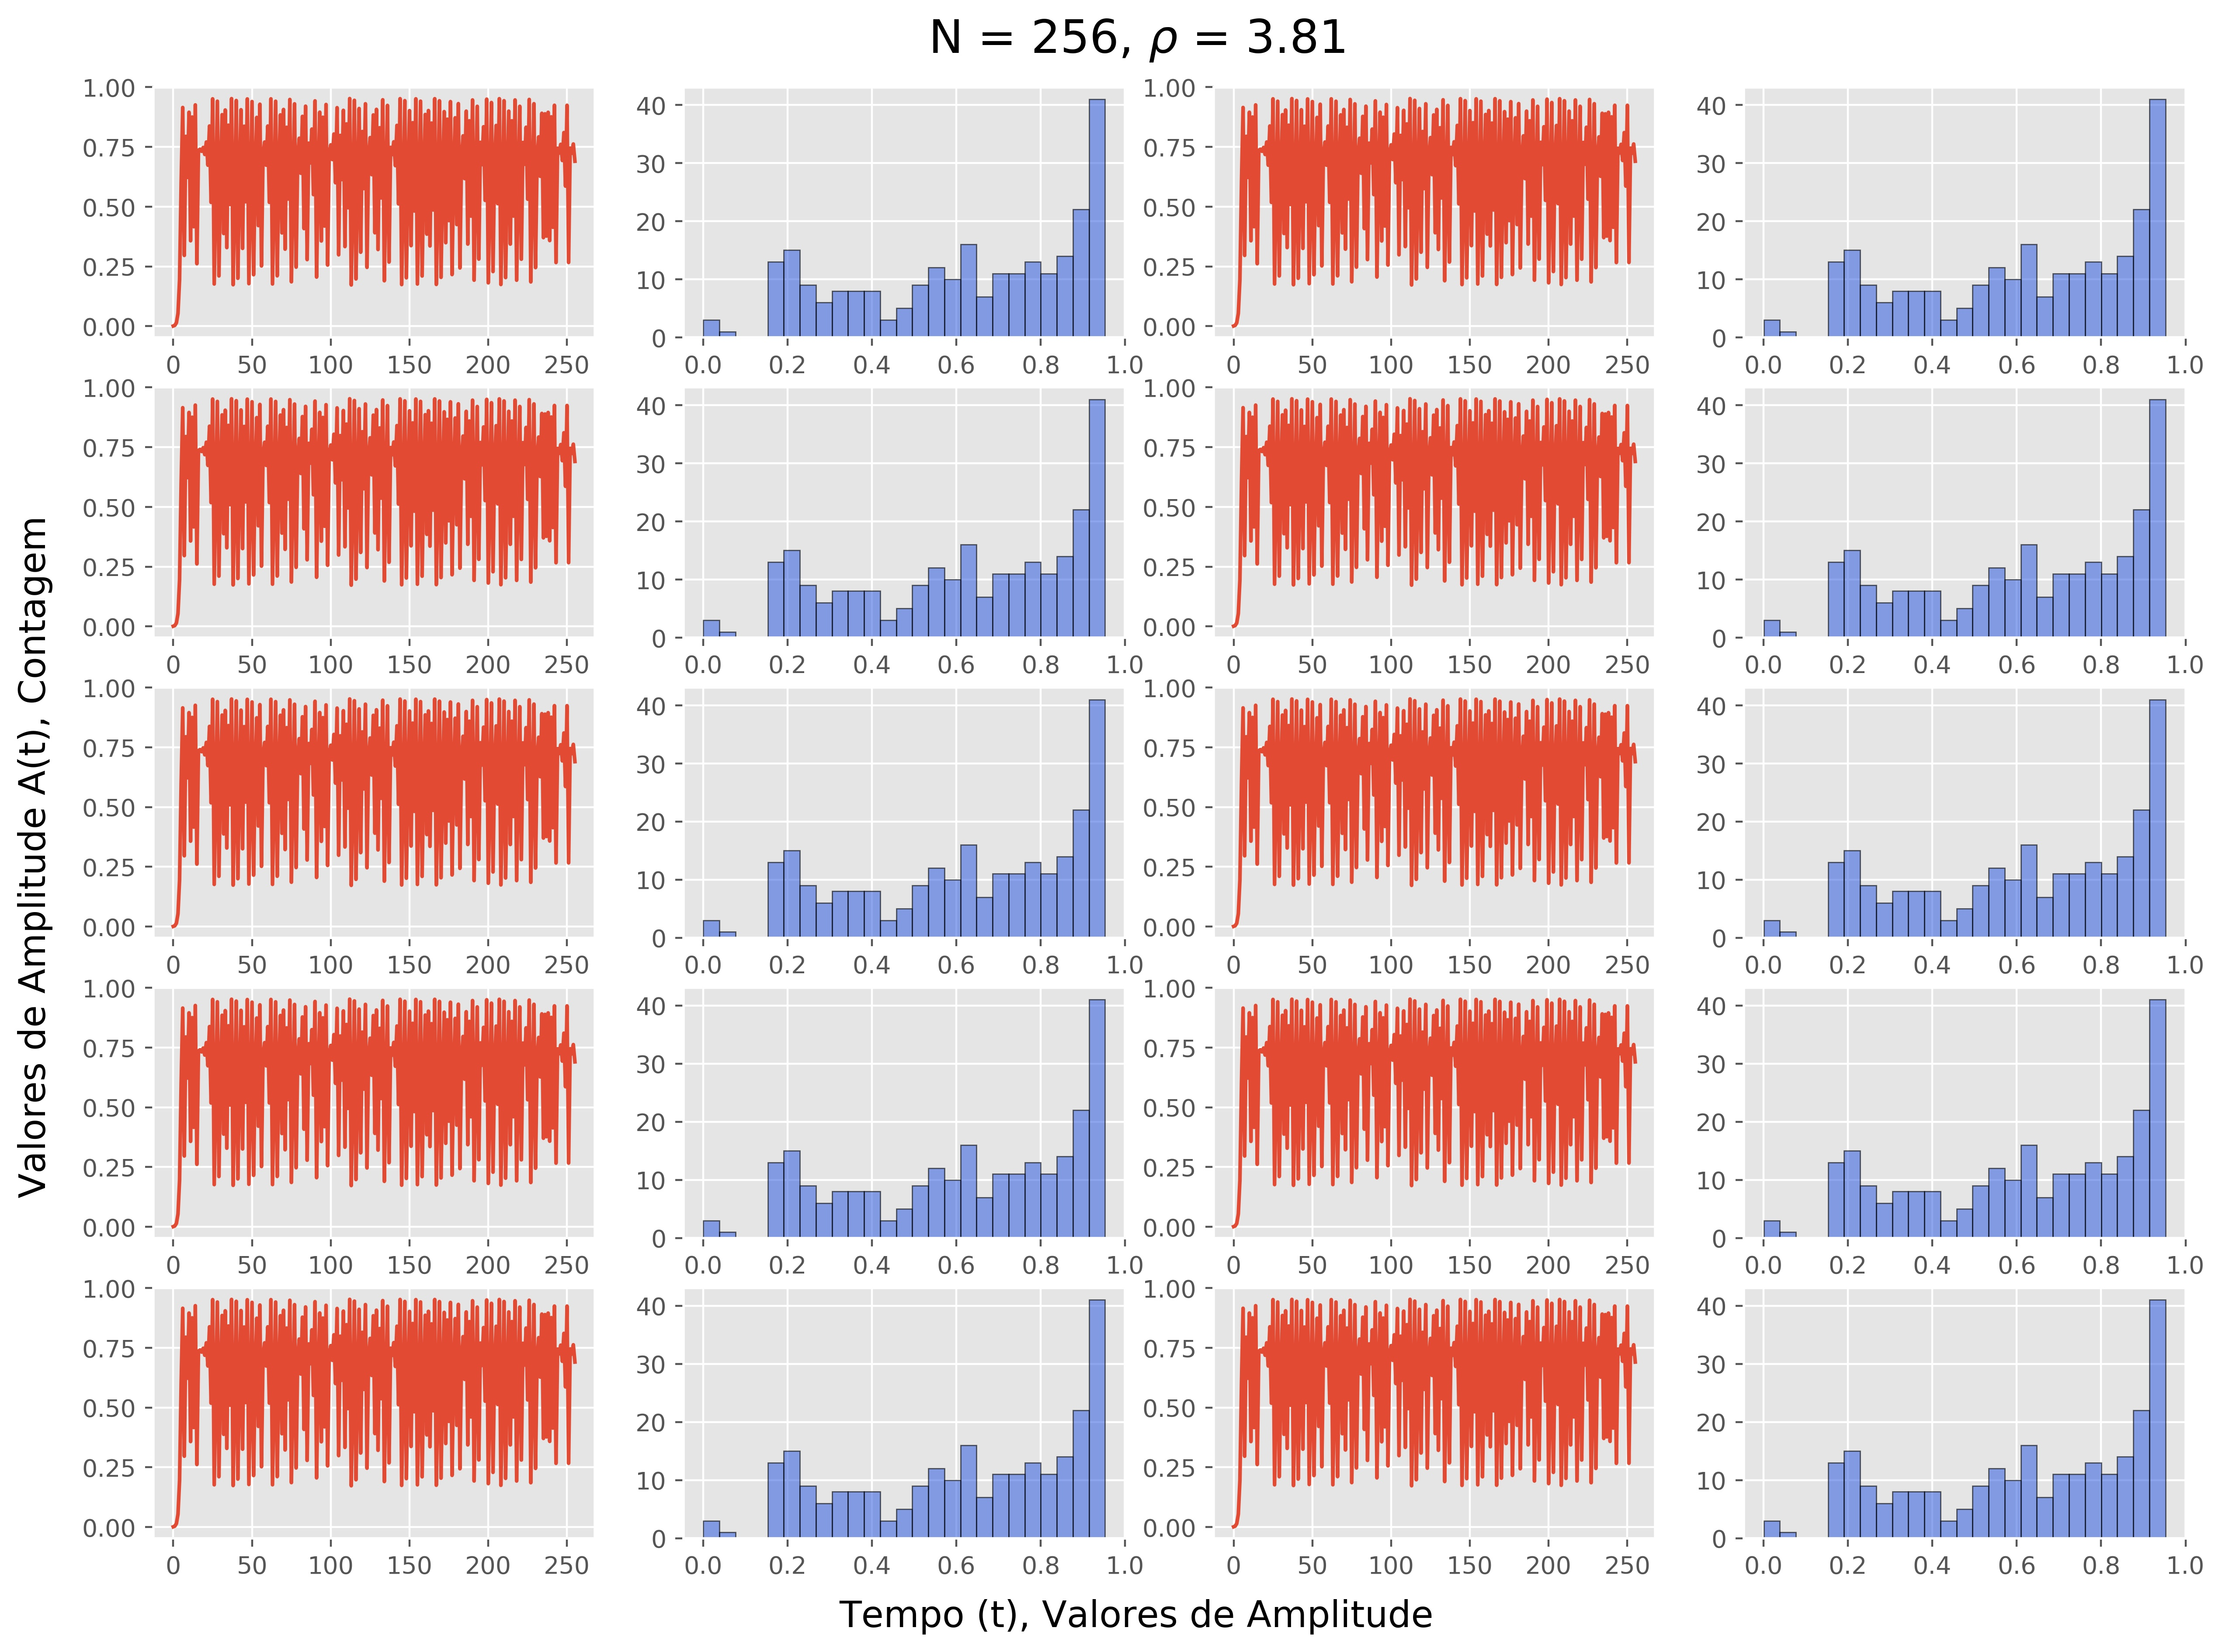
\includegraphics{Figuras/ex5/Logistico/Exercicio5_1_Logistico_n_256_rho_3.81.jpg}}		
	\end{center}
	\vspace{-2mm}	% acrescentar o espaçamento vertical apropriado entre a borda inferior da figura e a legenda ou a fonte quando não há legenda (o valor pode ser negativo para subir)
	\legenda{Figura 5.1.1: Plots de 10 sinais para a o mapeamento Logístico da família chaosnoise e seus respectivos histogramas. O tamanho da série foi de 256 para todos os valores de $\rho$. Acima os resultados para $\rho$ = 3.81.}	% legenda - para deixar sem legenda usar comando \legenda{} (nunca deve-se comentar o comando \legenda)
	\label{ex4_fig1}
	%\FONTE{}	% fonte consultada (elemento obrigatório, mesmo que seja produção do próprio autor)
\end{figure}

\clearpage
Os mesmos scripts da quarta questão foram implementados nas análises da família chaosnoise. A seguir são apresentados a classificação no espaço de Cullen and Frey e um ajuste de distribuições (incluindo GEV) a um dos sinais do mapeamento Logístico com $\rho$ = 3.81 (mais precisamente, o último sinal da Figura 5.1.1).

\begin{figure}[ht!]
	%\caption{Série e histogramas.}
	\vspace{0mm}	% acrescentar o espaçamento vertical apropriado entre o título e a borda superior da figura
	\begin{center}
		\resizebox{16cm}{!}{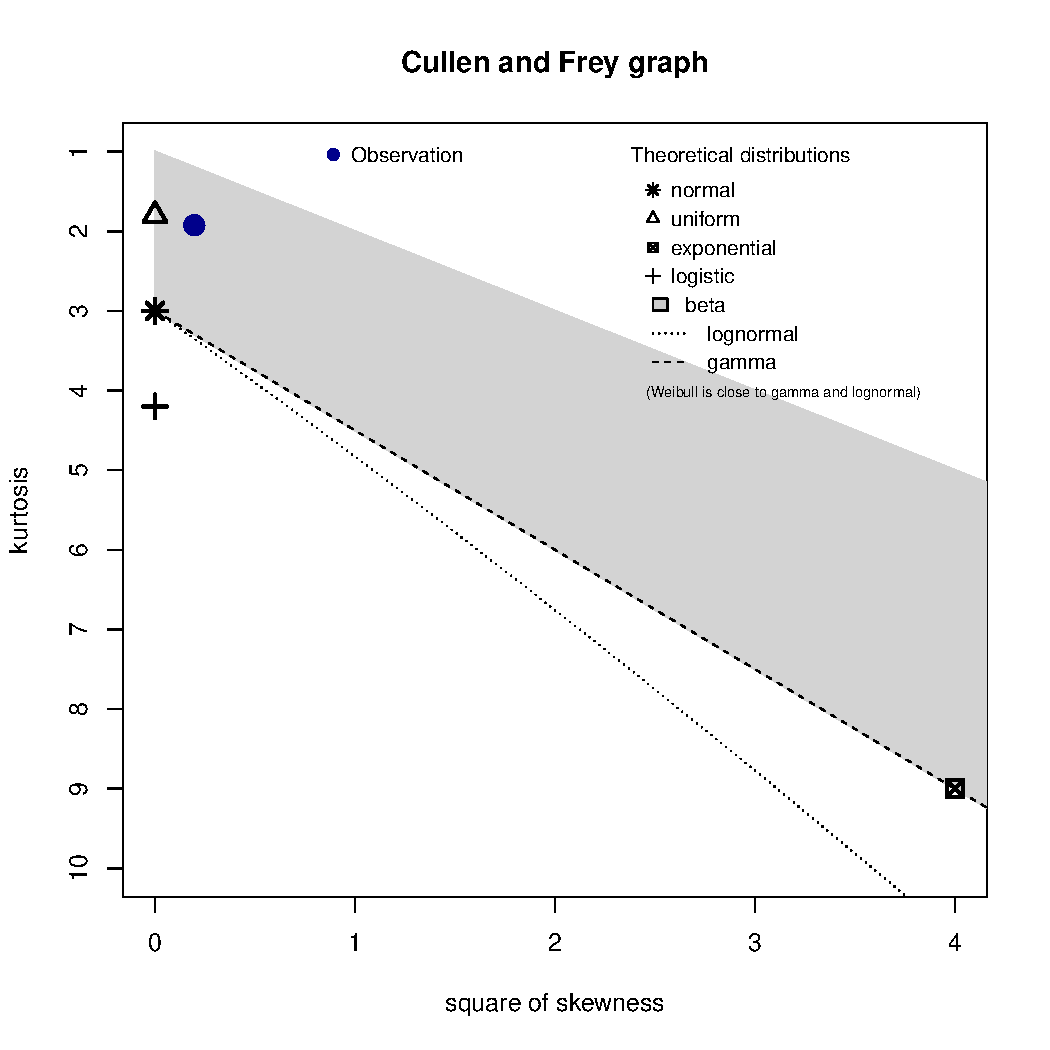
\includegraphics{Figuras/ex5/Logistico/rho_3.81_CullenFrey.pdf}}		
	\end{center}
	\vspace{-2mm}	% acrescentar o espaçamento vertical apropriado entre a borda inferior da figura e a legenda ou a fonte quando não há legenda (o valor pode ser negativo para subir)
	\legenda{Figura 5.1.2: Resultado da análise no espaço de Cullen and Frey para o mapeamento Logístico com $N$ = 256 e $\rho$ = 3.81 (último sinal da Figura 5.1.1).}	% legenda - para deixar sem legenda usar comando \legenda{} (nunca deve-se comentar o comando \legenda)
	\label{ex4_fig1}
	%\FONTE{}	% fonte consultada (elemento obrigatório, mesmo que seja produção do próprio autor)
\end{figure}

\clearpage

\begin{figure}[ht!]
	%\caption{Série e histogramas.}
	\vspace{0mm}	% acrescentar o espaçamento vertical apropriado entre o título e a borda superior da figura
	\begin{center}
		\resizebox{13cm}{!}{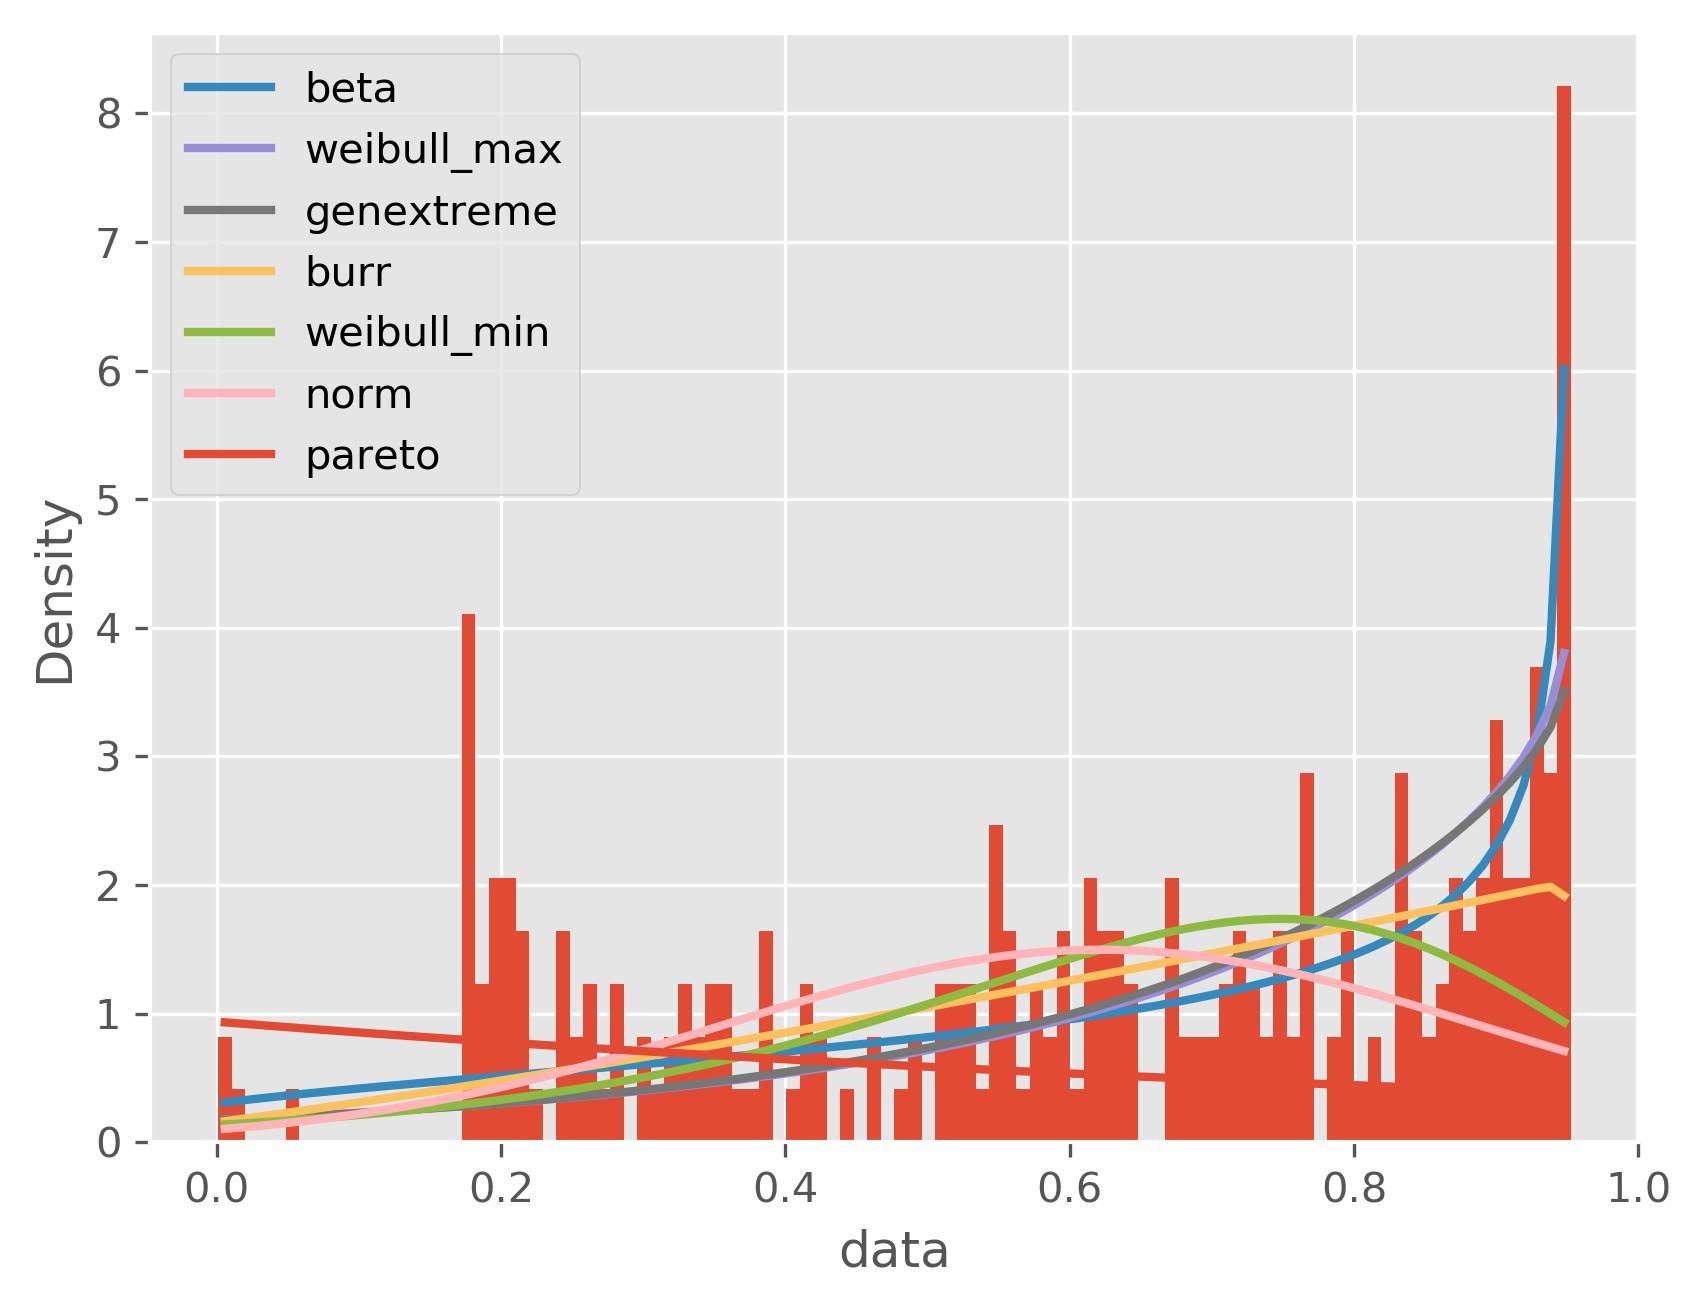
\includegraphics{Figuras/ex5/Logistico/rho_3.81_Python_fits.jpg}}		
	\end{center}
	\vspace{-2mm}	% acrescentar o espaçamento vertical apropriado entre a borda inferior da figura e a legenda ou a fonte quando não há legenda (o valor pode ser negativo para subir)
	\legenda{Figura 5.1.3: Resultado do ajuste de 7 distribuições ao último sinal presente na Figura 5.1.1.}	% legenda - para deixar sem legenda usar comando \legenda{} (nunca deve-se comentar o comando \legenda)
	\label{ex4_fig1}
	%\FONTE{}	% fonte consultada (elemento obrigatório, mesmo que seja produção do próprio autor)
\end{figure}

Resultado do benchmark do ajuste das distribuições. Observa-se que a distribuição \texttt{beta} foi a de melhor ajuste. Esse resultado se encontra no arquivo \textit{rho\_3.81\_Python\_fits.txt}.

\begin{figure}[ht!]
	%\caption{Série e histogramas.}
	\vspace{0mm}	% acrescentar o espaçamento vertical apropriado entre o título e a borda superior da figura
	%\begin{center}
		\resizebox{13cm}{!}{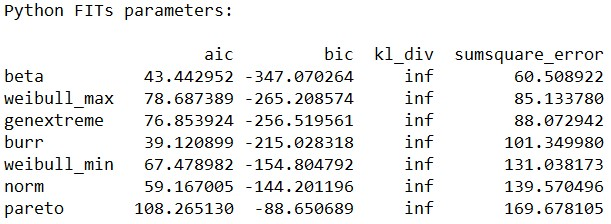
\includegraphics{Figuras/ex5/Logistico/rho_3.81_Python_fits_params.jpg}}		
	%\end{center}
	\vspace{-2mm}	% acrescentar o espaçamento vertical apropriado entre a borda inferior da figura e a legenda ou a fonte quando não há legenda (o valor pode ser negativo para subir)
	%\legenda{Figura 5.3:.}	% legenda - para deixar sem legenda usar comando \legenda{} (nunca deve-se comentar o comando \legenda)
	\label{ex4_fig1}
	%\FONTE{}	% fonte consultada (elemento obrigatório, mesmo que seja produção do próprio autor)
\end{figure}

%%%%%%%%%%%%%%%%%%%%%%%%%%%%%%%%%%% Henon %%%%%%%%%%%%%%%%%%%%%%%%%%%%%%%%%%%%%%%%%%

\clearpage
\subsubsection*{Henon}
Para o mapeamento de Henon, os valores de $a$ escolhidos foram 1.32 e 1.4. Para $b$, escolheu-se os valores 0.21, 0.26 e 0.31, de forma a fixar o primeiro e variar o segundo gerando-se cinco sinais para cada combinação de parâmetros.


\begin{figure}[ht!]
  \begin{adjustbox}{addcode={\begin{minipage}{\width}}{\\% 
      Figura 5.1.4: Série de 15 sinais diferentes (e seus respectivos histogramas) gerados com o script chaosnoise.py. A figura exibe o resultado de $a$ = 1.32 e três valores de $b$. Os cinco primeiros sinais (da esquerda) são para $b$ = 0.21, os cinco do centro para $b$ = 0.26, e os cinco da direita para $b$ = 0.31.
      \end{minipage}},rotate=90,center}
      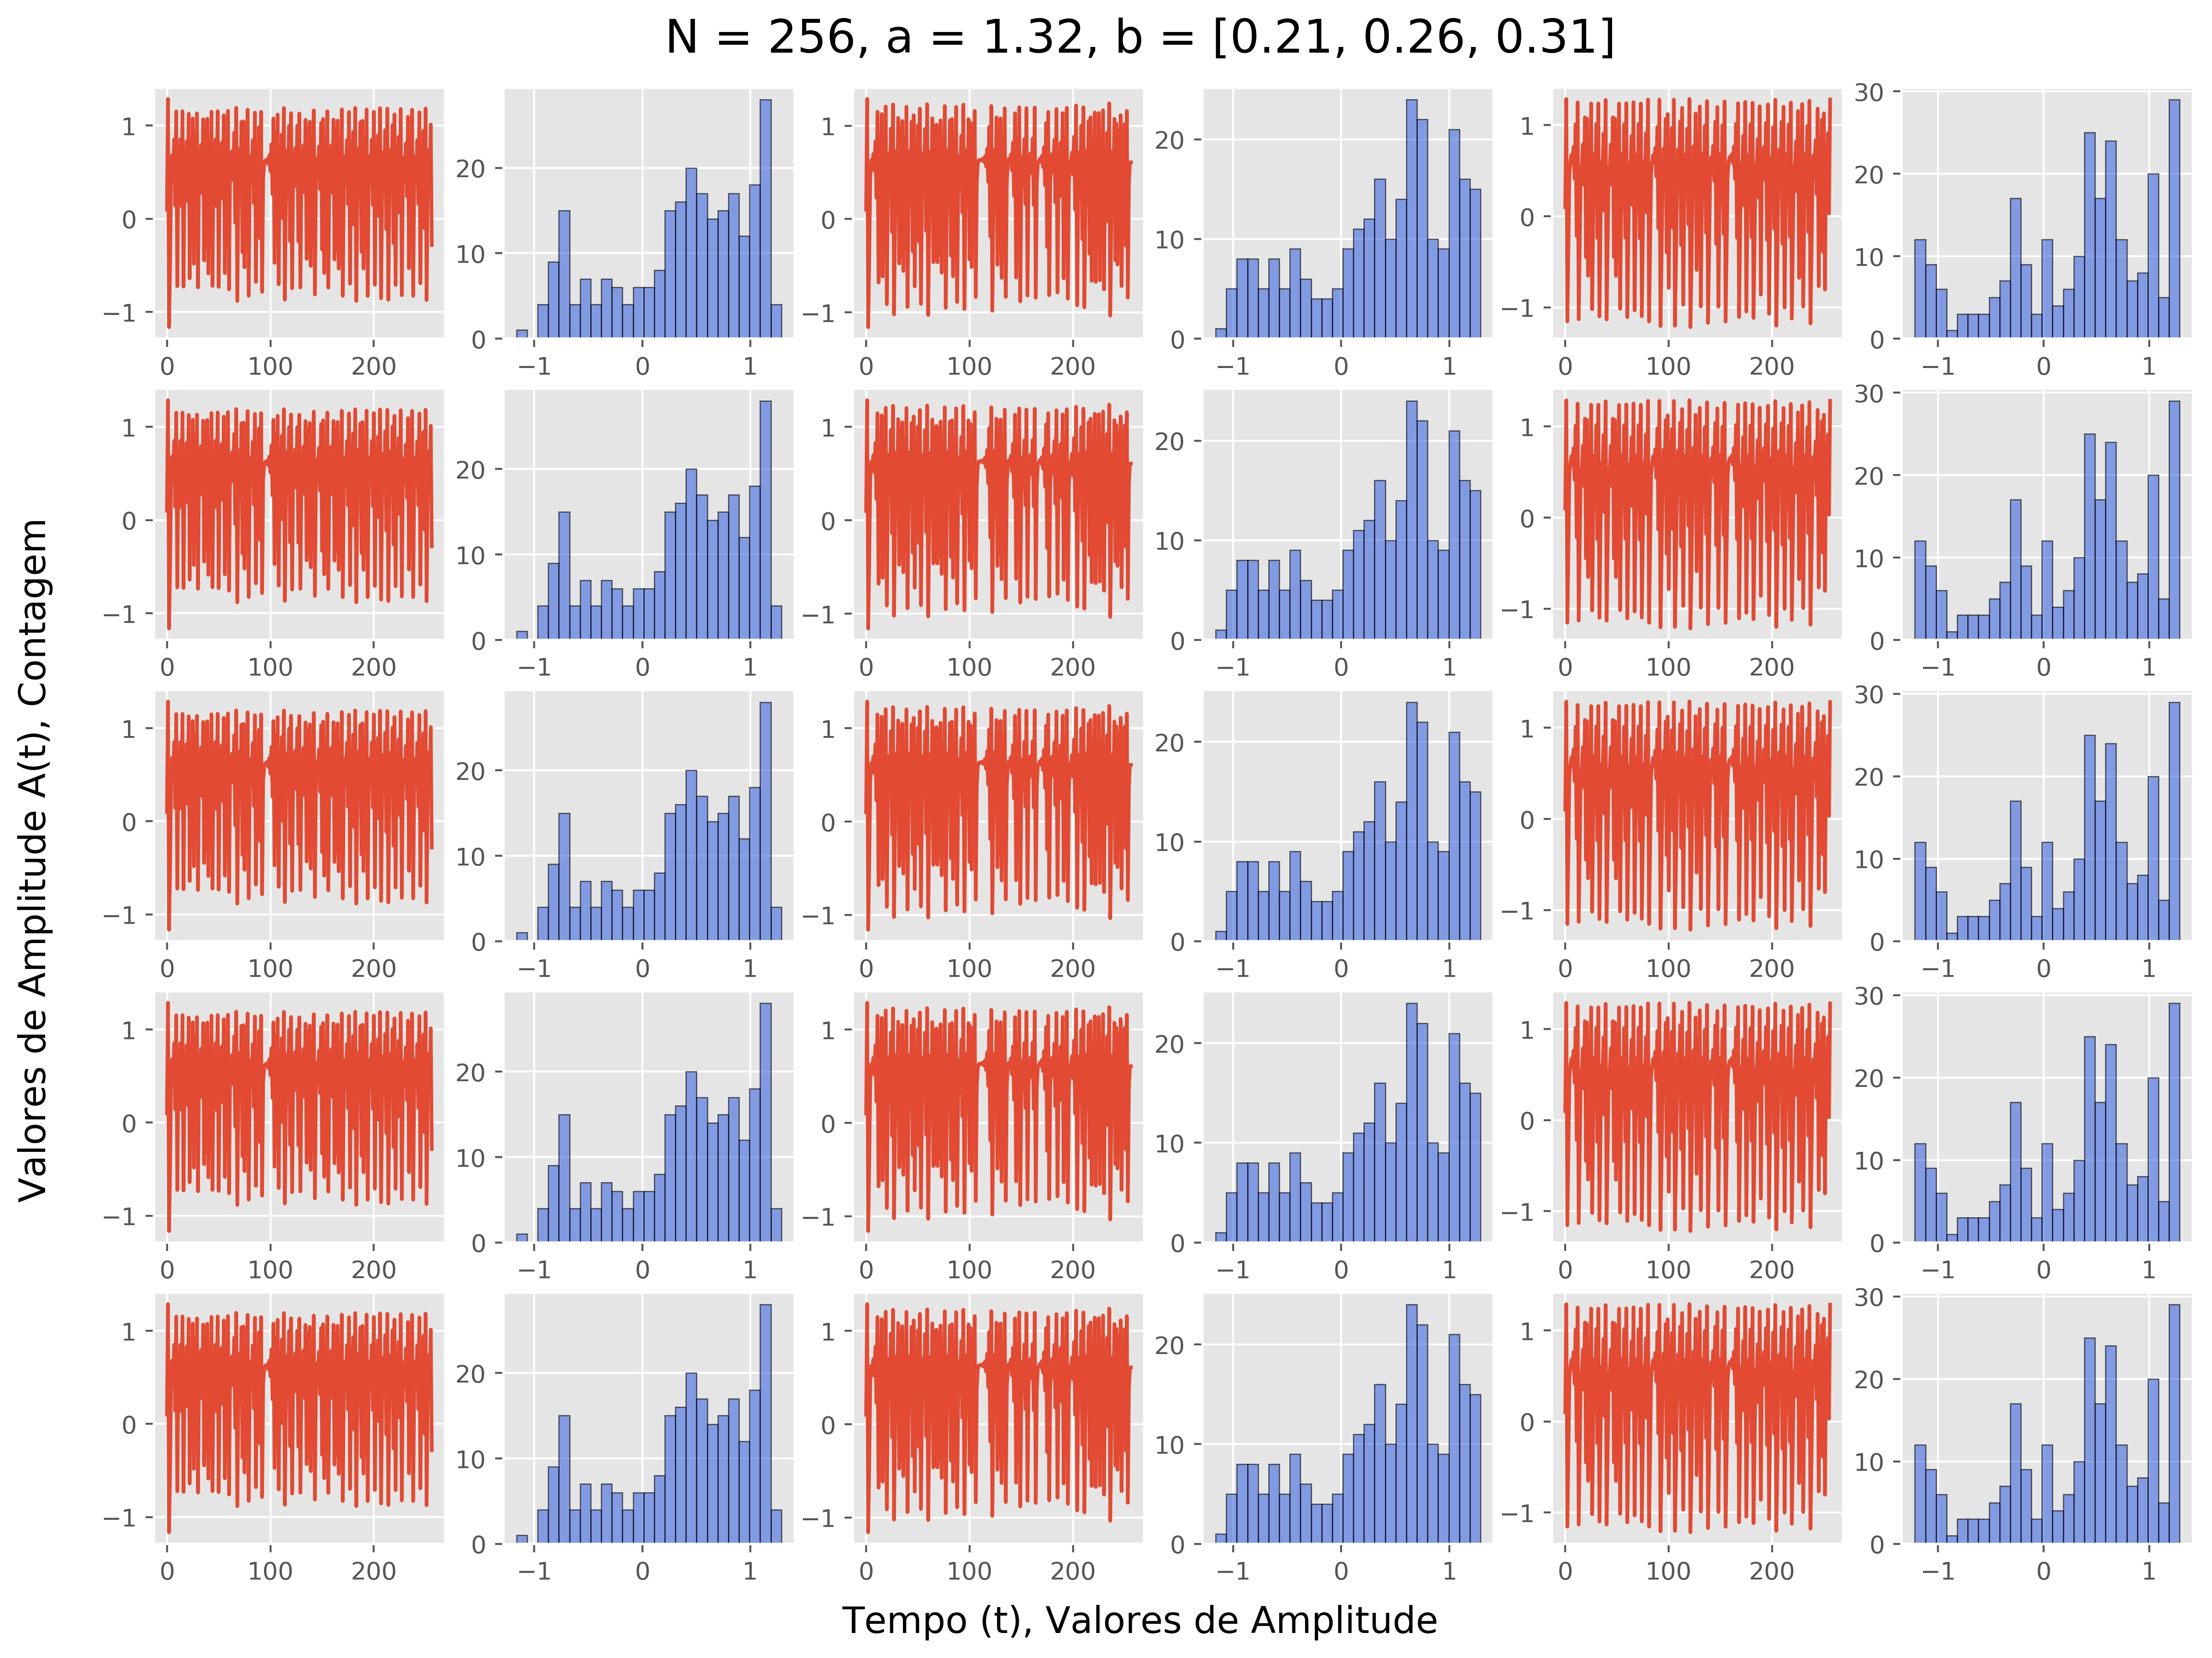
\includegraphics[scale=.5]{Figuras/ex5/Henon/Exercicio5_1_Henon_n_256_a_1.32.jpg}	%
  \end{adjustbox}
\end{figure}

%\begin{figure}[ht!]
%	%\caption{Série e histogramas.}
%	\vspace{0mm}	% acrescentar o espaçamento vertical apropriado entre o título e a borda superior da figura
%	\begin{center}
%		\resizebox{17cm}{!}{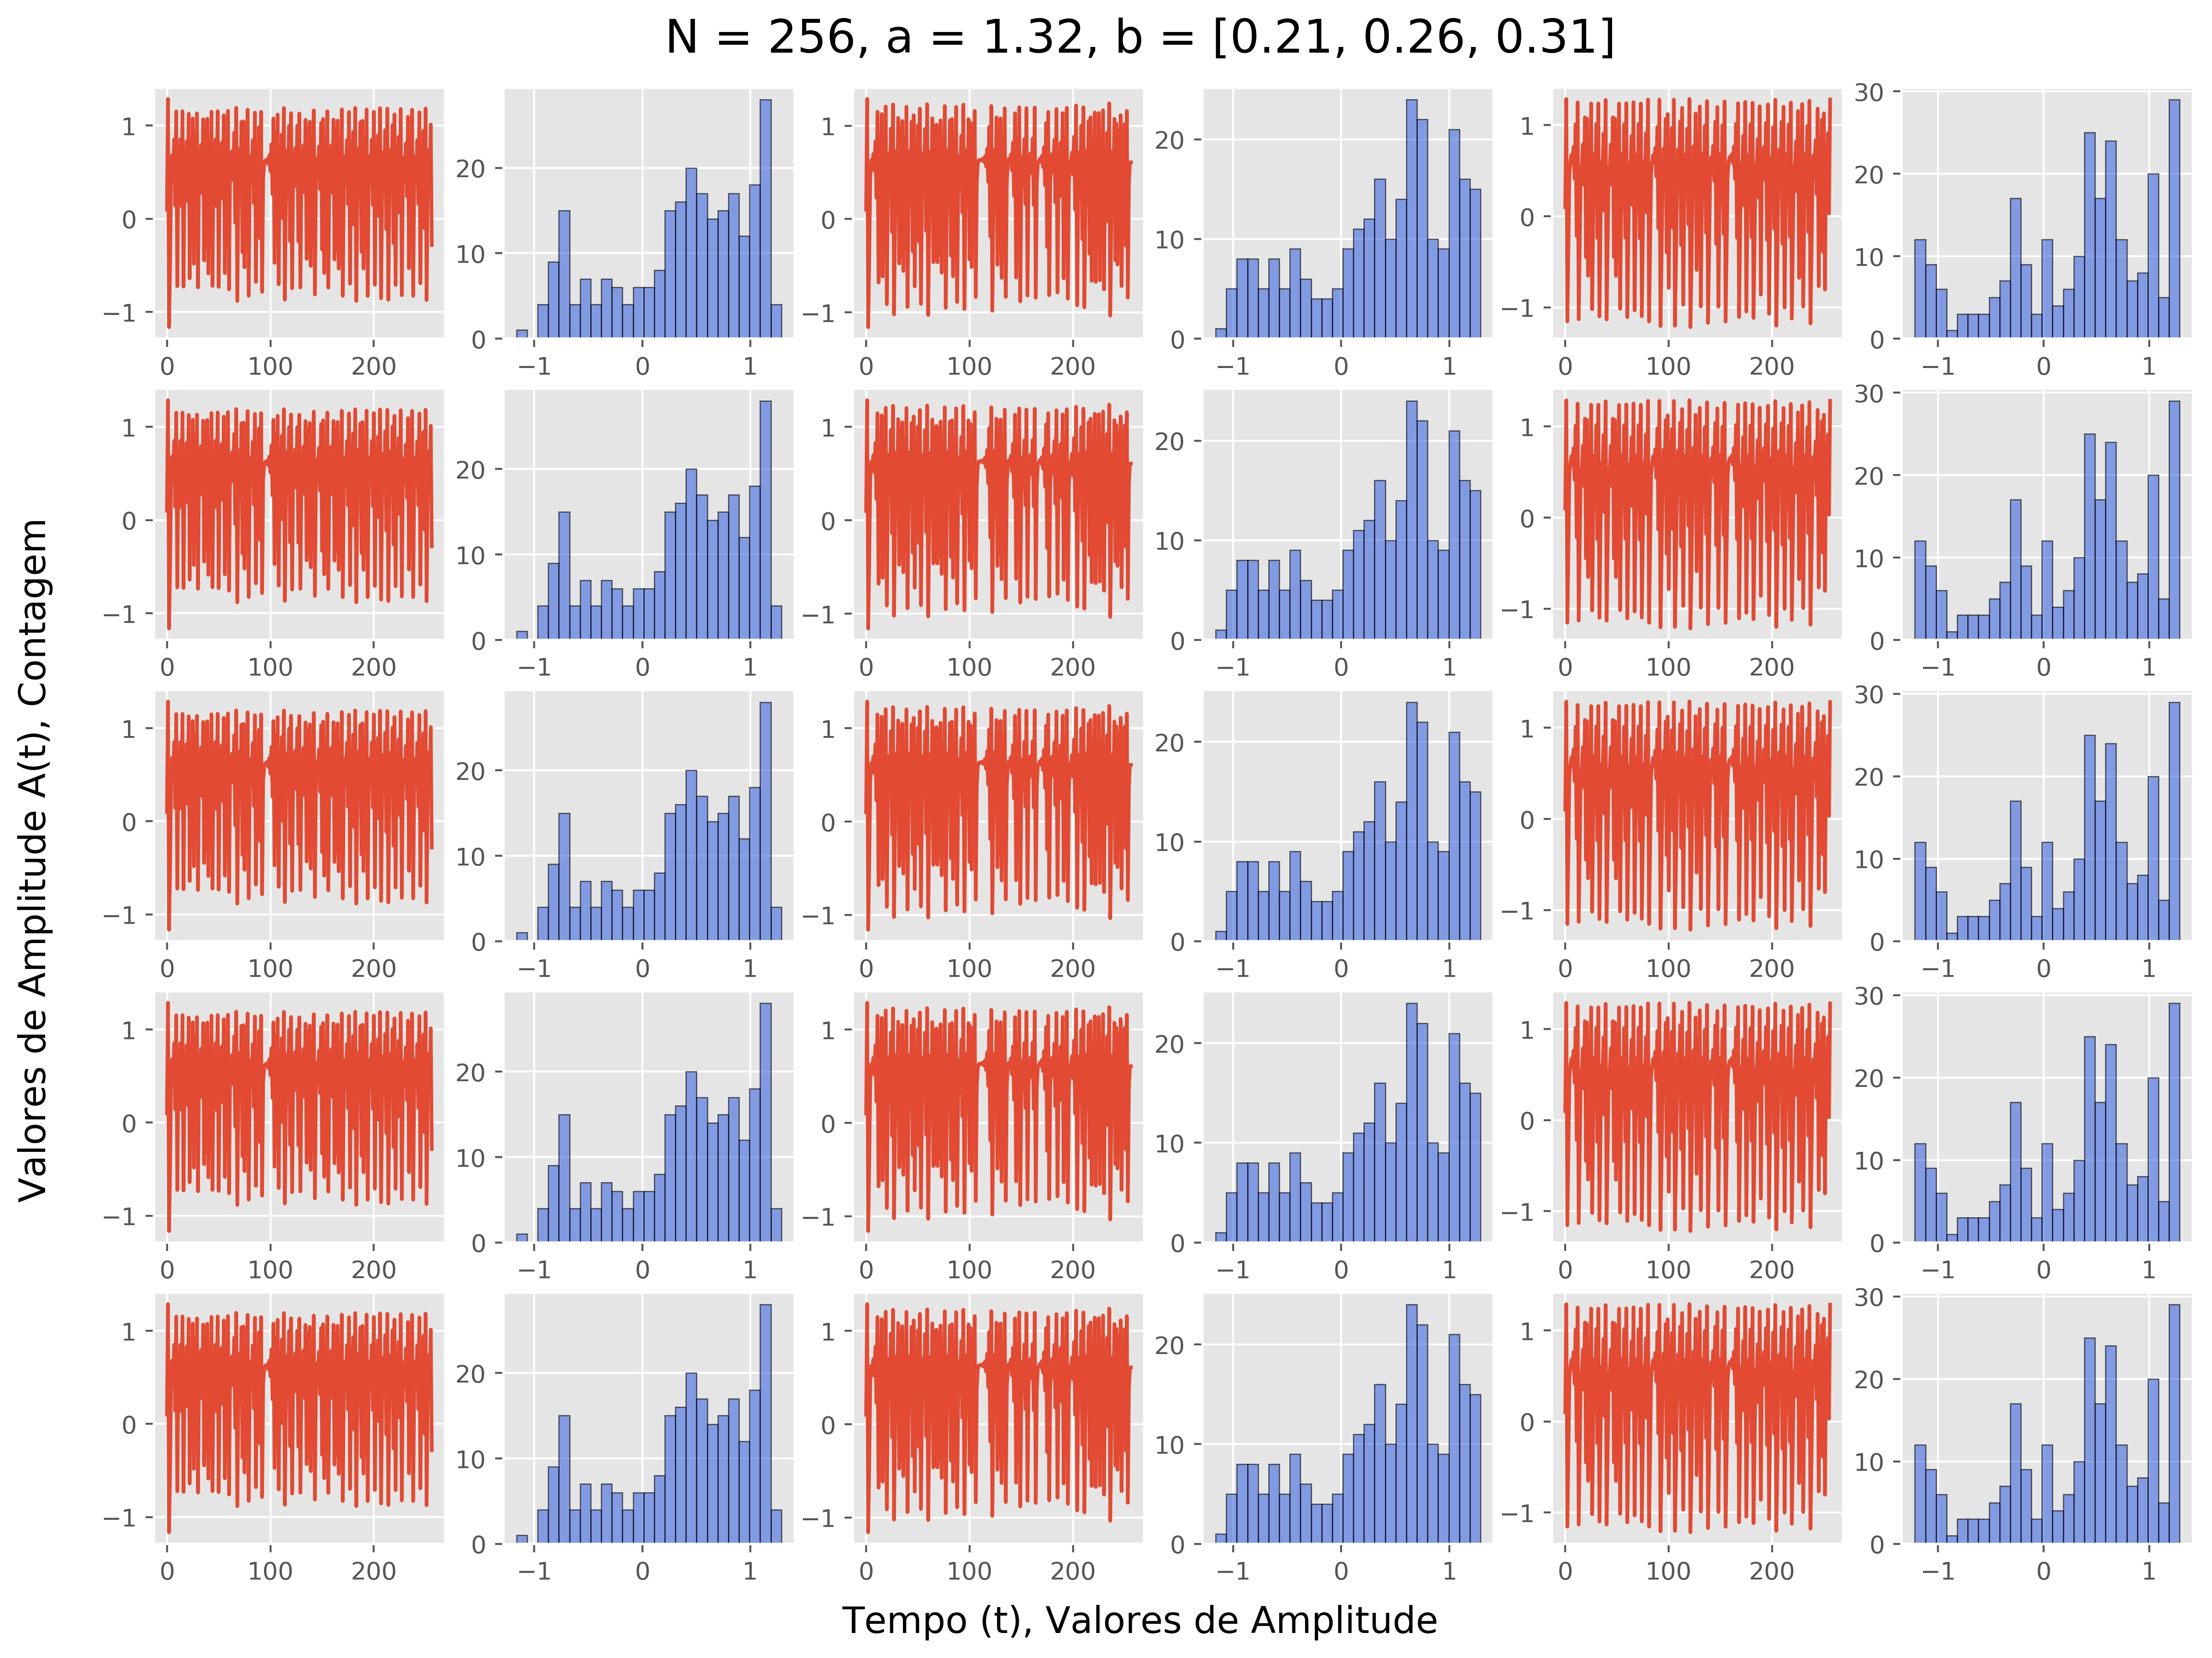
\includegraphics{Figuras/ex5/Henon/Exercicio5_1_Henon_n_256_a_1.32.jpg}}		
%	\end{center}
%	\vspace{-2mm}	% acrescentar o espaçamento vertical apropriado entre a borda inferior da figura e a legenda ou a fonte quando não há legenda (o valor pode ser negativo para subir)
%	\legenda{Figura 5.1.4:.}	% legenda - para deixar sem legenda usar comando \legenda{} (nunca deve-se comentar o comando \legenda)
%	\label{ex4_fig1}
	%\FONTE{}	% fonte consultada (elemento obrigatório, mesmo que seja produção do próprio autor)
%\end{figure}

A seguir são apresentados a classificação no espaço de Cullen and Frey e um ajuste de distribuições (incluindo GEV) a um dos sinais do mapeamento de Henon com $a$ = 1.32 e $b$ = 0.31 (mais precisamente, o último sinal da Figura 5.1.4).

\begin{figure}[ht!]
	%\caption{Série e histogramas.}
	\vspace{0mm}	% acrescentar o espaçamento vertical apropriado entre o título e a borda superior da figura
	\begin{center}
		\resizebox{16cm}{!}{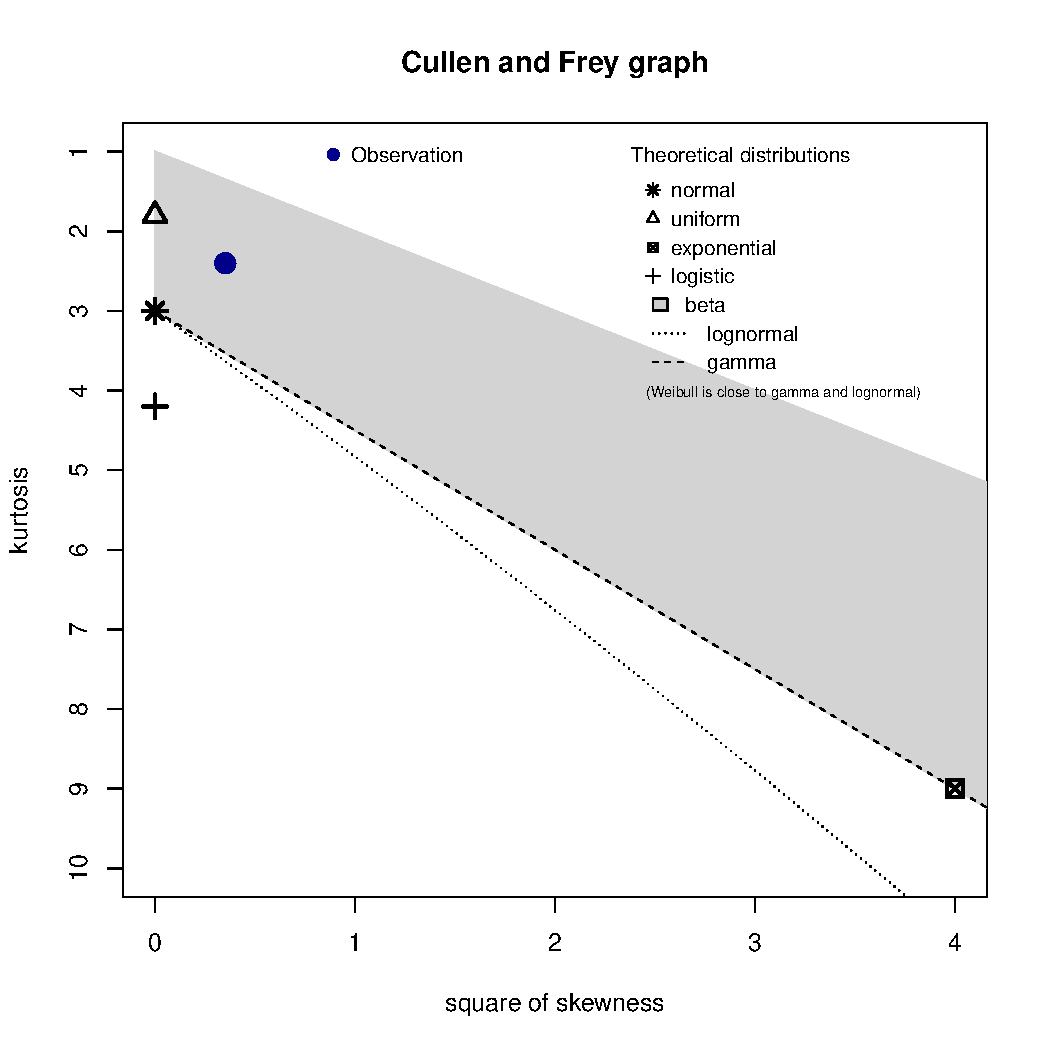
\includegraphics{Figuras/ex5/Henon/a_1.32_b_0.31_CullenFrey.pdf}}		
	\end{center}
	\vspace{-2mm}	% acrescentar o espaçamento vertical apropriado entre a borda inferior da figura e a legenda ou a fonte quando não há legenda (o valor pode ser negativo para subir)
	\legenda{Figura 5.1.5: Resultado da análise no espaço de Cullen and Frey para o mapeamento de Henon com $a$ = 1.32 e $b$ = 0.31 (último sinal da Figura 5.1.4).}	% legenda - para deixar sem legenda usar comando \legenda{} (nunca deve-se comentar o comando \legenda)
	\label{ex4_fig1}
	%\FONTE{}	% fonte consultada (elemento obrigatório, mesmo que seja produção do próprio autor)
\end{figure}

\clearpage 

\begin{figure}[ht!]
	%\caption{Série e histogramas.}
	\vspace{0mm}	% acrescentar o espaçamento vertical apropriado entre o título e a borda superior da figura
	\begin{center}
		\resizebox{13cm}{!}{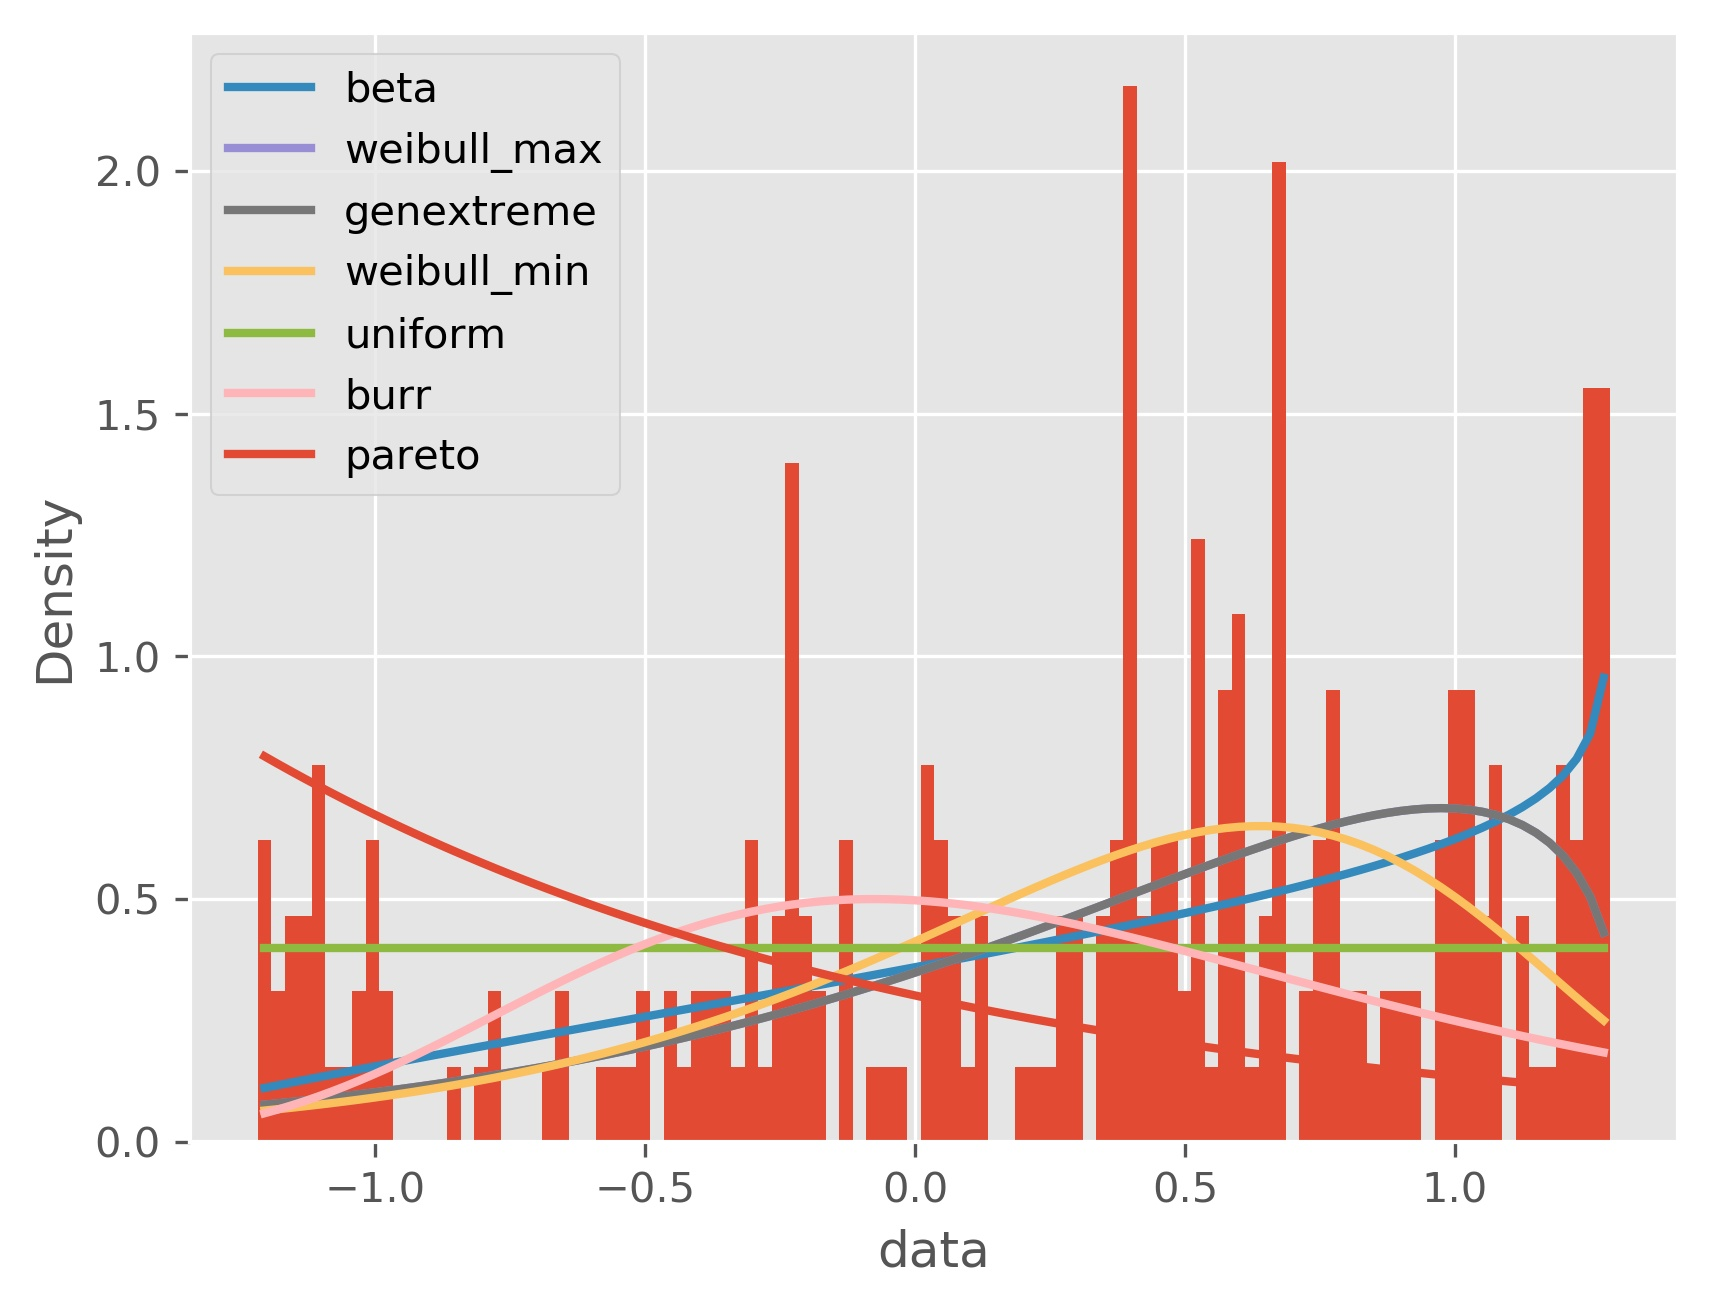
\includegraphics{Figuras/ex5/Henon/a_1.32_b_0.31_Python_fits.jpg}}		
	\end{center}
	\vspace{-2mm}	% acrescentar o espaçamento vertical apropriado entre a borda inferior da figura e a legenda ou a fonte quando não há legenda (o valor pode ser negativo para subir)
	\legenda{Figura 5.1.6: Resultado do ajuste de 7 distribuições ao último sinal presente na Figura 5.1.4.}	% legenda - para deixar sem legenda usar comando \legenda{} (nunca deve-se comentar o comando \legenda)
	\label{ex4_fig1}
	%\FONTE{}	% fonte consultada (elemento obrigatório, mesmo que seja produção do próprio autor)
\end{figure}

Resultado do benchmark do ajuste das distribuições. Novamente, observa-se que a distribuição \texttt{beta} foi a de melhor ajuste. Esse resultado se encontra no arquivo \textit{a\_1.32\_b\_0.31\_Python\_fits.txt}.

\begin{figure}[ht!]
	%\caption{Série e histogramas.}
	\vspace{0mm}	% acrescentar o espaçamento vertical apropriado entre o título e a borda superior da figura
	%\begin{center}
		\resizebox{13cm}{!}{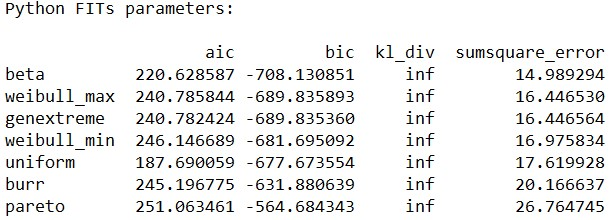
\includegraphics{Figuras/ex5/Henon/a_1.32_b_0.31_Python_fits_params.jpg}}		
	%\end{center}
	\vspace{-2mm}	% acrescentar o espaçamento vertical apropriado entre a borda inferior da figura e a legenda ou a fonte quando não há legenda (o valor pode ser negativo para subir)
	%\legenda{Figura 5.3:.}	% legenda - para deixar sem legenda usar comando \legenda{} (nunca deve-se comentar o comando \legenda)
	\label{ex4_fig1}
	%\FONTE{}	% fonte consultada (elemento obrigatório, mesmo que seja produção do próprio autor)
\end{figure}

%%%%%%%%%%%%%%%%%%%%%%%%%%%%%%%%%%%%%%%%% 5.2 %%%%%%%%%%%%%%%%%%%%%%%%%%%%%%%%%%%%%%%%%%

\clearpage
\subsection*{5.2}
\addcontentsline{toc}{section}{\protect\numberline{} 5.2}%

A segunda lei de Newton é definida por:

\begin{equation*}
\sum\vec{f}_{ext} = m \vec{a},
\end{equation*}

que representa que a aceleração de um corpor é devido ao somatório das forças externas aplicadas à ele. Para uma parcela de fluido de densidade $\rho$, a força por unidade de volume é

\begin{equation*}
\sum\vec{f} = \rho \vec{a} = \vec{f}_{grav} + \vec{f}_{press} + \vec{f}_{visc},
\end{equation*}

onde $\vec{f}_{grav}$ = $\rho\vec{g}$ é a força gravitacional, agindo sobre o fluido na direção negativa de $\vec{z}$, ou seja, para baixo; $\vec{f}_{press}$ = $-\vec{\nabla}p$ representa as forças de pressão, agindo sobre o fluido em todas as direções, para o seu interior e normal à sua superfície; $\vec{f}_{visc}$ = $\mu \nabla^{2} \vec{v}$ denota a força viscosa, que 
é proporcional à velocidade $v$ do fluido e age em sua superfície (normalmente ou tangencialmente) por conta da viscosidade $\mu$ do mesmo ($\nabla^{2}$ é o operador Laplaciano).

Expandindo a aceleração, escrevendo-a em termos de derivadas dos componentes da velocidade, e substituindo cada um dos componentes de força atuando sobre a parcela de fluido, temos

\begin{equation*}
\rho \left( \frac{\partial \vec{v}}{\partial t} + \vec{v}_{x}\frac{\partial \vec{v}}{\partial x} + \vec{v}_{y}\frac{\partial \vec{v}}{\partial y} + \vec{v}_{z}\frac{\partial \vec{v}}{\partial z} \right) = \rho\vec{g} - \vec{\nabla}p + \mu \nabla^{2} \vec{v},
\end{equation*}

que é a equação de \textit{Navier-Stokes} válida para fluidos Newtonianos incompressíveis.  %% 1o capítulo, começo do texto

\clearpage
%%%%%%%%%%%%%%%%%%%%%%%%%%%%%%%%%%%%%%%%%%%%%%%%%%%%%%%%%%%%%%%%%%%%%%%%%%%%%%%

\section*{\large Exercício 6 - PSD \& DFA}
\addcontentsline{toc}{chapter}{\protect\numberline{}\large Exercício 6}%

Os resultados deste exercício se encontram na pasta \textbf{Exercise6} organizados nas pastas \textbf{6.1}, \textbf{6.2} e \textbf{6.3}. 
%Por usa vez, \textbf{6.1} e \textbf{6.2} contém (cada uma) seus resultados em diretórios distintos para cada grupo da tabela \textit{Dataset\_signal}. 

\subsection*{6.1.}
\addcontentsline{toc}{section}{\protect\numberline{} 6.1}%

Como exemplo, a seguir estão os resultados da análise do grupo noise, pesentes na pasta \textbf{grupo\_noise} (dentro da pasta referente a este exercício - \textbf{6.1}).

\begin{figure}[ht!]
	%\caption{Série e histogramas.}
	\vspace{-4mm}	% acrescentar o espaçamento vertical apropriado entre o título e a borda superior da figura
	\begin{center}
		\resizebox{11cm}{!}{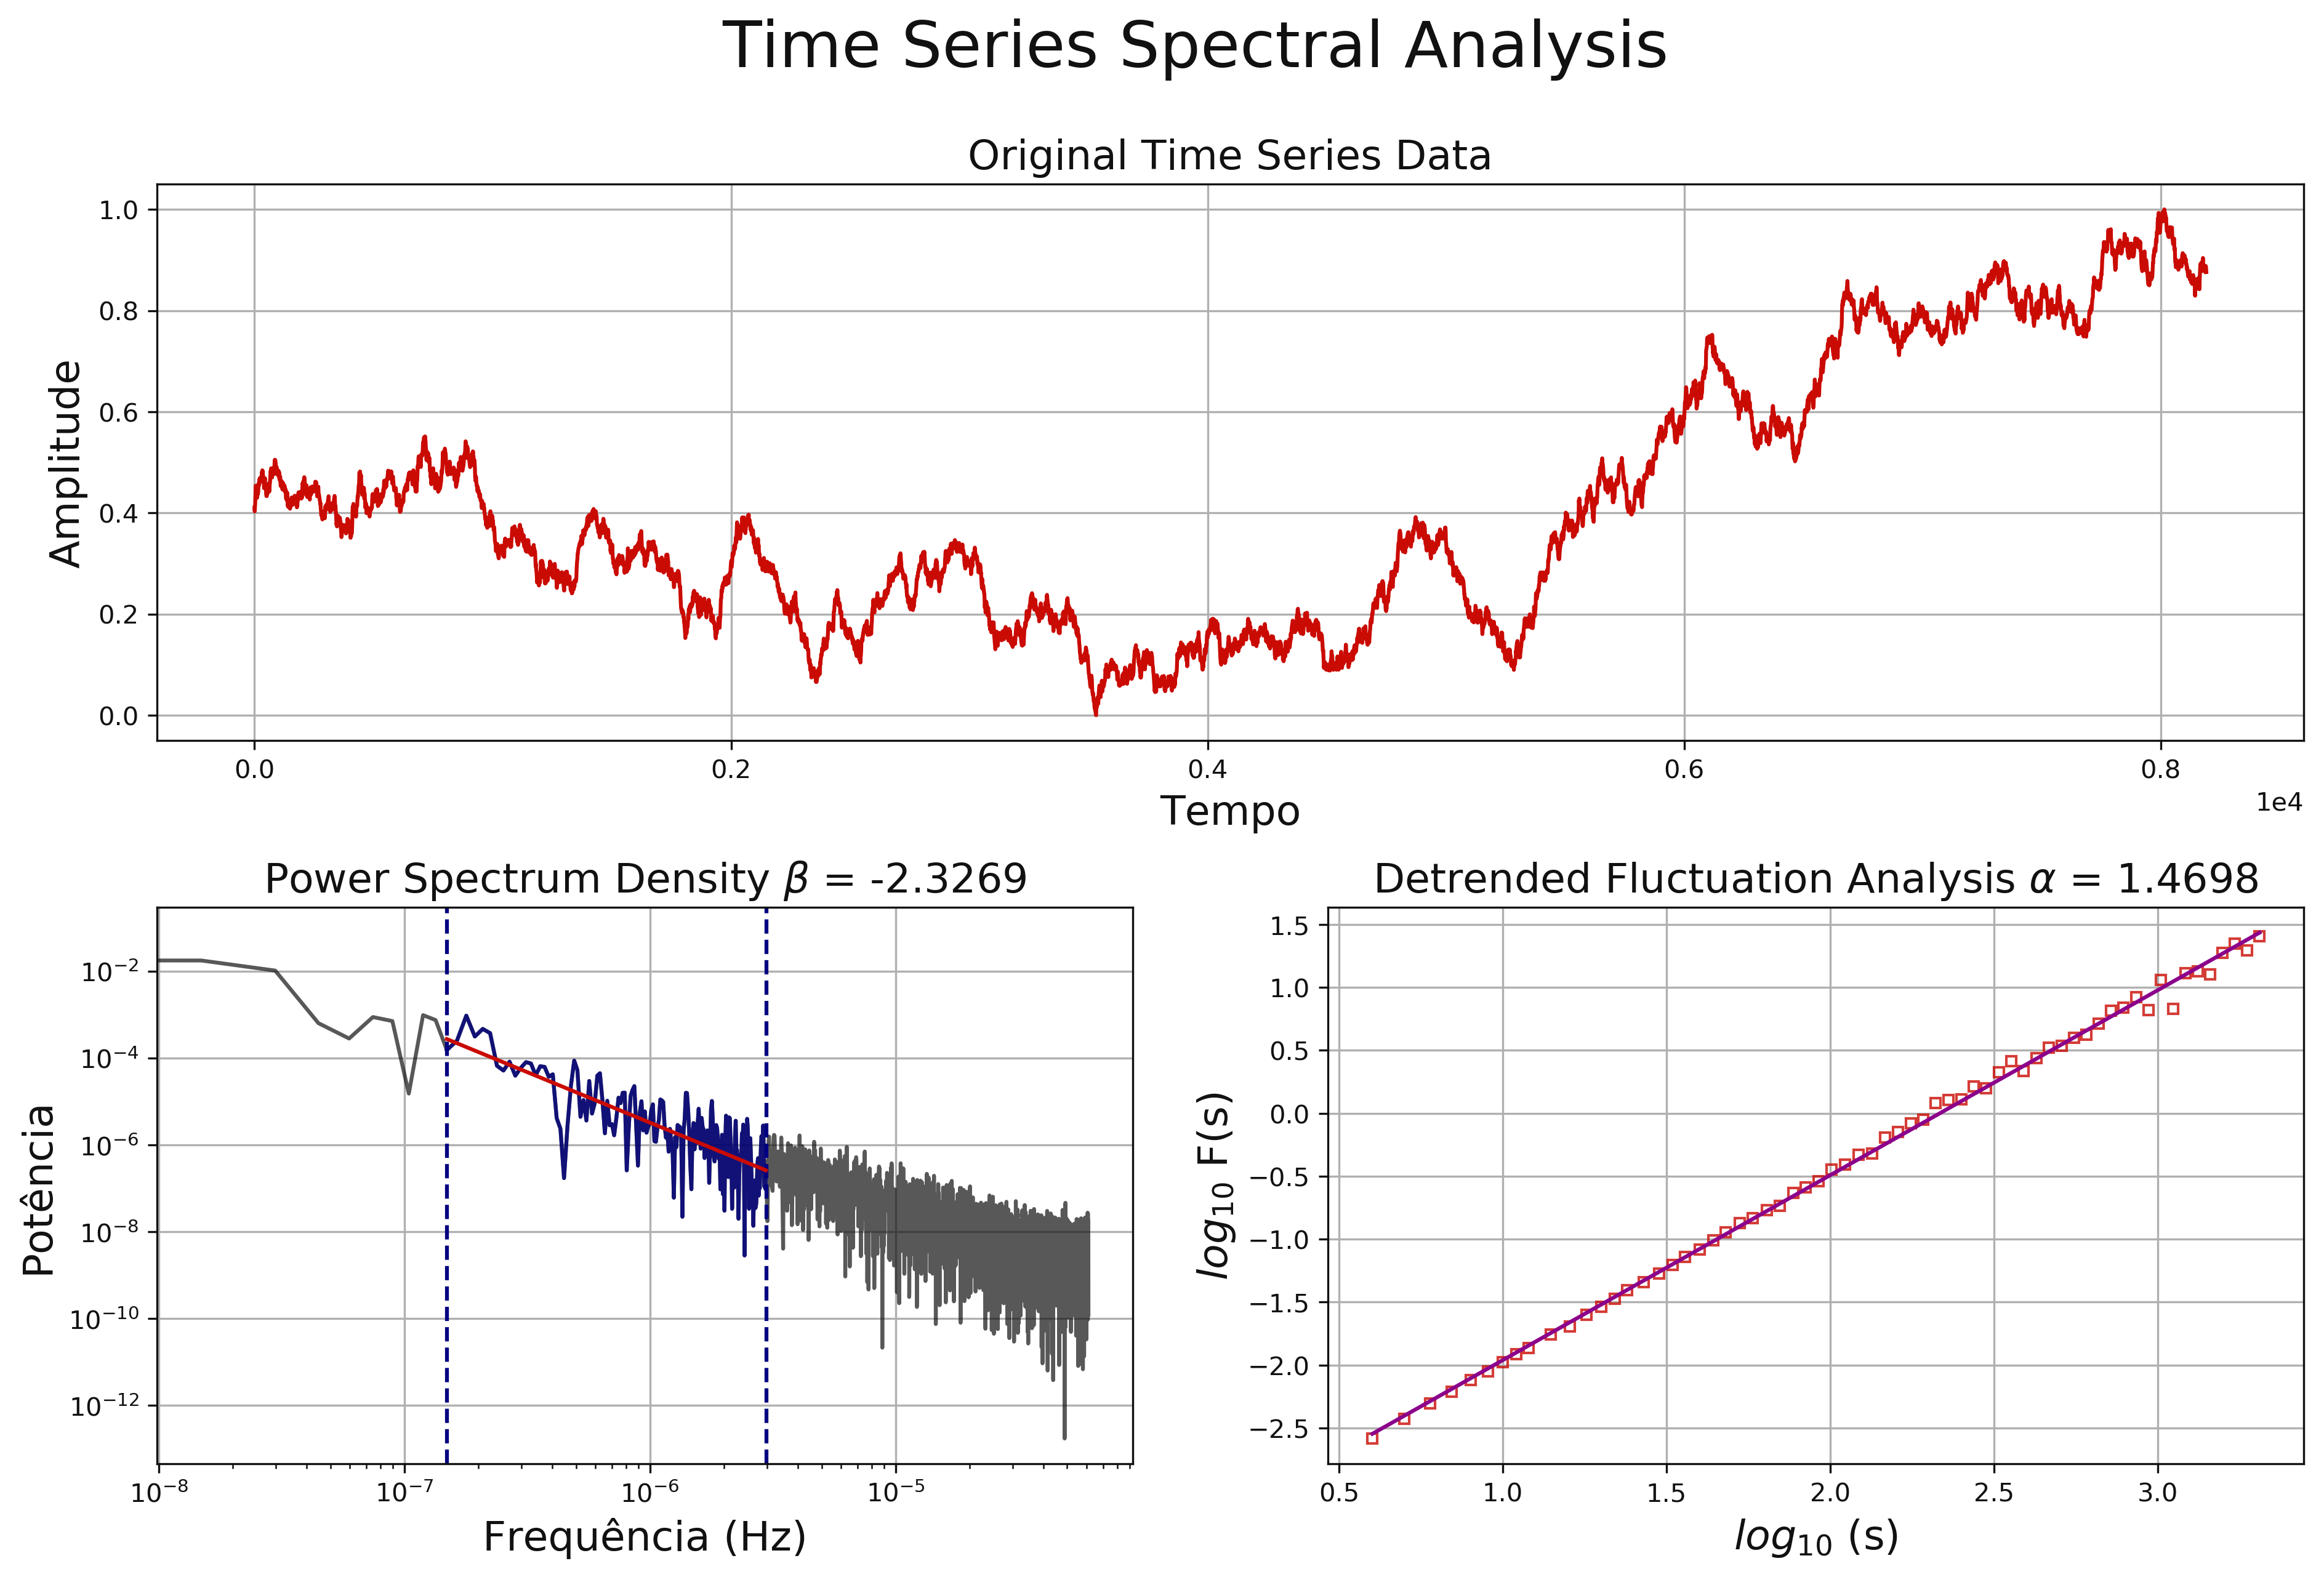
\includegraphics{Figuras/ex6/6_1/Exercicio6_1_grupo_noise_Specplus_n_8192.png}}		
	\end{center}
	\vspace{-2mm}	% acrescentar o espaçamento vertical apropriado entre a borda inferior da figura e a legenda ou a fonte quando não há legenda (o valor pode ser negativo para subir)
	\legenda{Figura 6.1.1: Acima, sinal do grupo noise com $n$ = 8192; abaixo à esquerda, o PSD e o índice espectral $\beta \sim$ -2.32; abaixo à direita, o DFA com o expoente de escala $\alpha \sim$ 1.47.}	% legenda - para deixar sem legenda usar comando \legenda{} (nunca deve-se comentar o comando \legenda)
	\label{ex6_fig1}
	%\FONTE{}	% fonte consultada (elemento obrigatório, mesmo que seja produção do próprio autor)
\end{figure}

\begin{figure}[ht!]
	%\caption{Série e histogramas.}
	\vspace{-3mm}	% acrescentar o espaçamento vertical apropriado entre o título e a borda superior da figura
	\begin{center}
		\resizebox{8cm}{!}{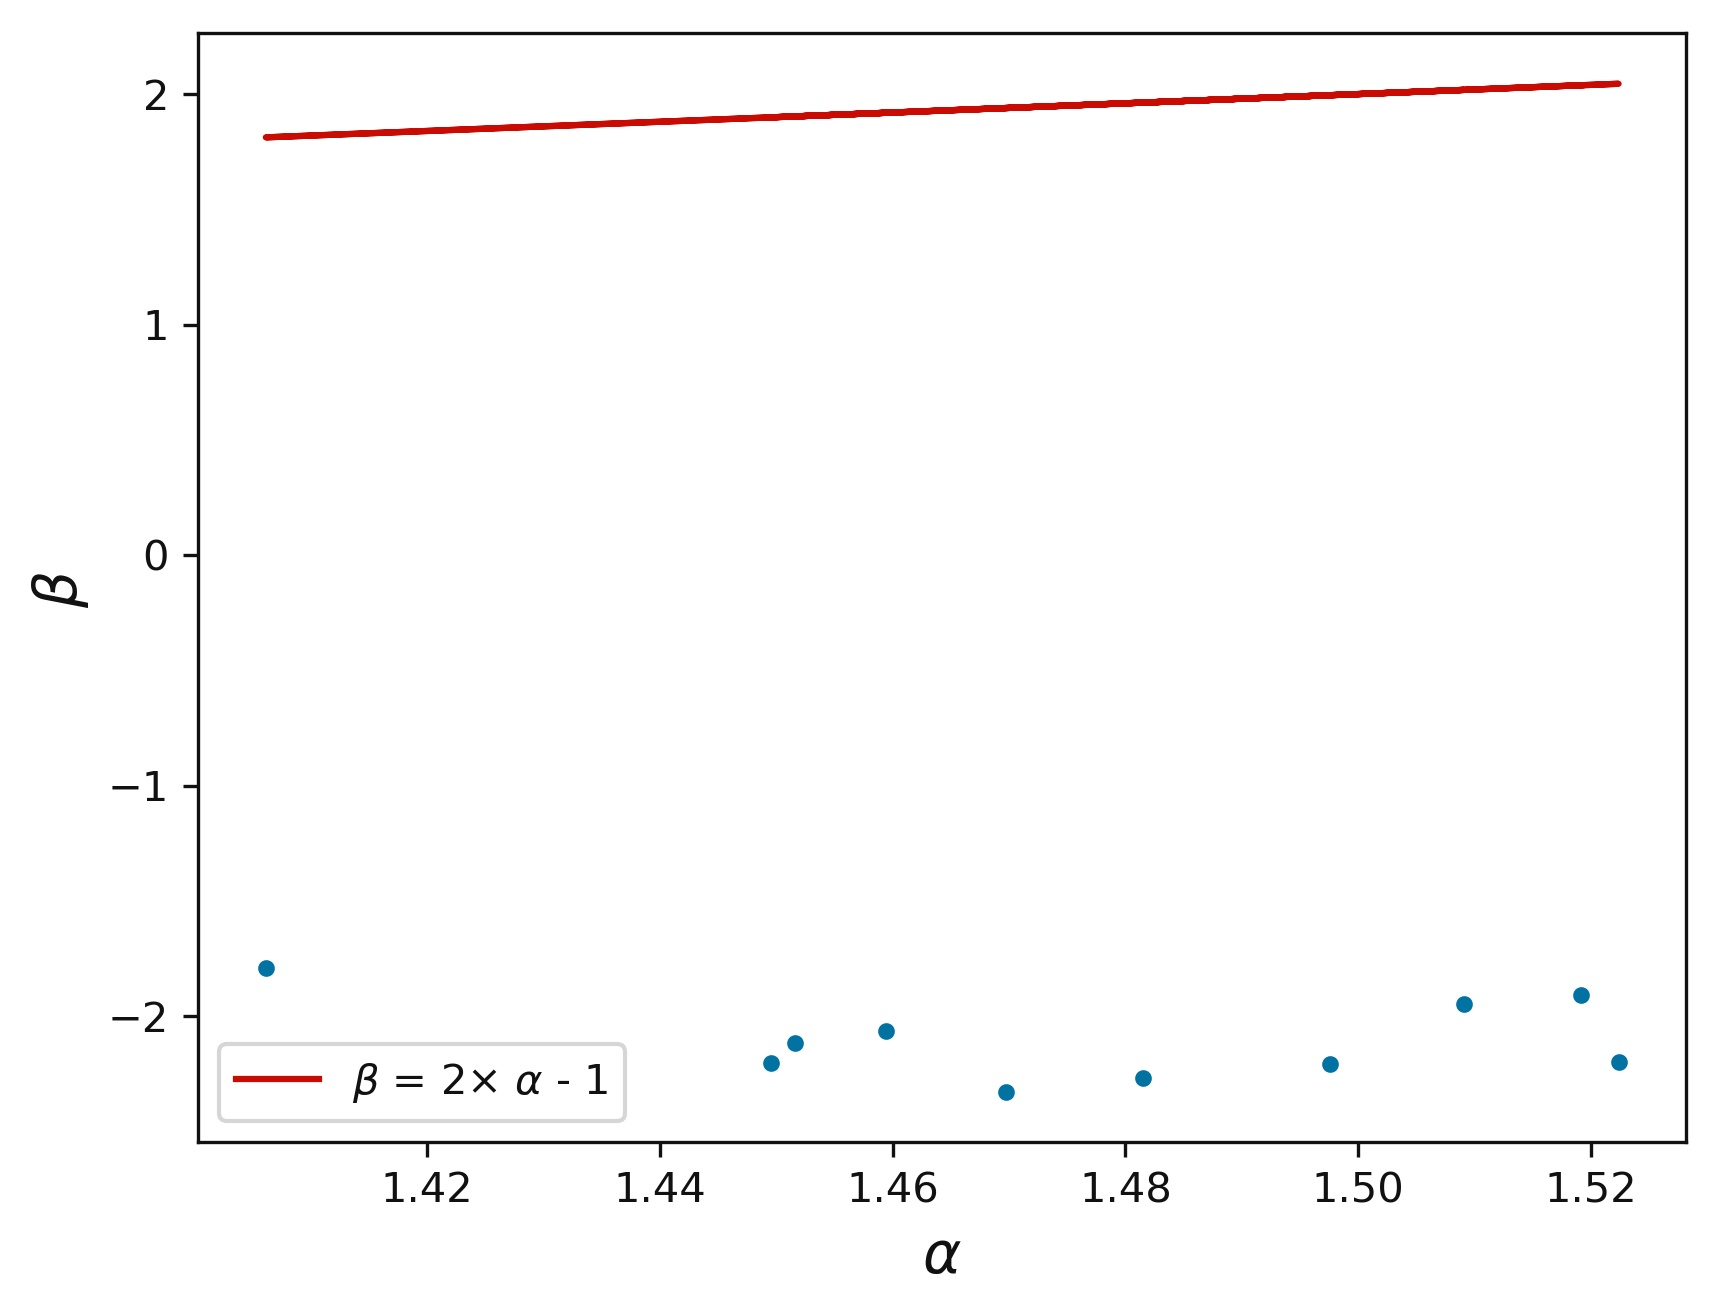
\includegraphics{Figuras/ex6/6_1/Exercicio6_1_grupo_noise_alfa_vs_beta_n_8192.jpg}}		
	\end{center}
	\vspace{-3mm}	% acrescentar o espaçamento vertical apropriado entre a borda inferior da figura e a legenda ou a fonte quando não há legenda (o valor pode ser negativo para subir)
	\legenda{Figura 6.1.2: Resultado do teste do ajuste dos valores de $\beta$ e $\alpha$ para a família noise com $n$ = 8192 à equação do Teorema de Wiener–Khinchin-Parseval. Os pontos são valores empíricos. A reta é o resultado da equação do Teorema de WKP sobre os $\alpha$'s empíricos. Observa-se que, em módulo, o $\beta$ teórico é compatível com o empírico.}	% legenda - para deixar sem legenda usar comando \legenda{} (nunca deve-se comentar o comando \legenda)
	\label{ex6_fig2}
	%\FONTE{}	% fonte consultada (elemento obrigatório, mesmo que seja produção do próprio autor)
\end{figure}

\clearpage
Primeiro resultado do agrupamento kmeans do grupo noise (usando $\beta$):

\begin{figure}[ht!]
	%\caption{Série e histogramas.}
	\vspace{-3mm}	% acrescentar o espaçamento vertical apropriado entre o título e a borda superior da figura
	\begin{center}
		\resizebox{14cm}{!}{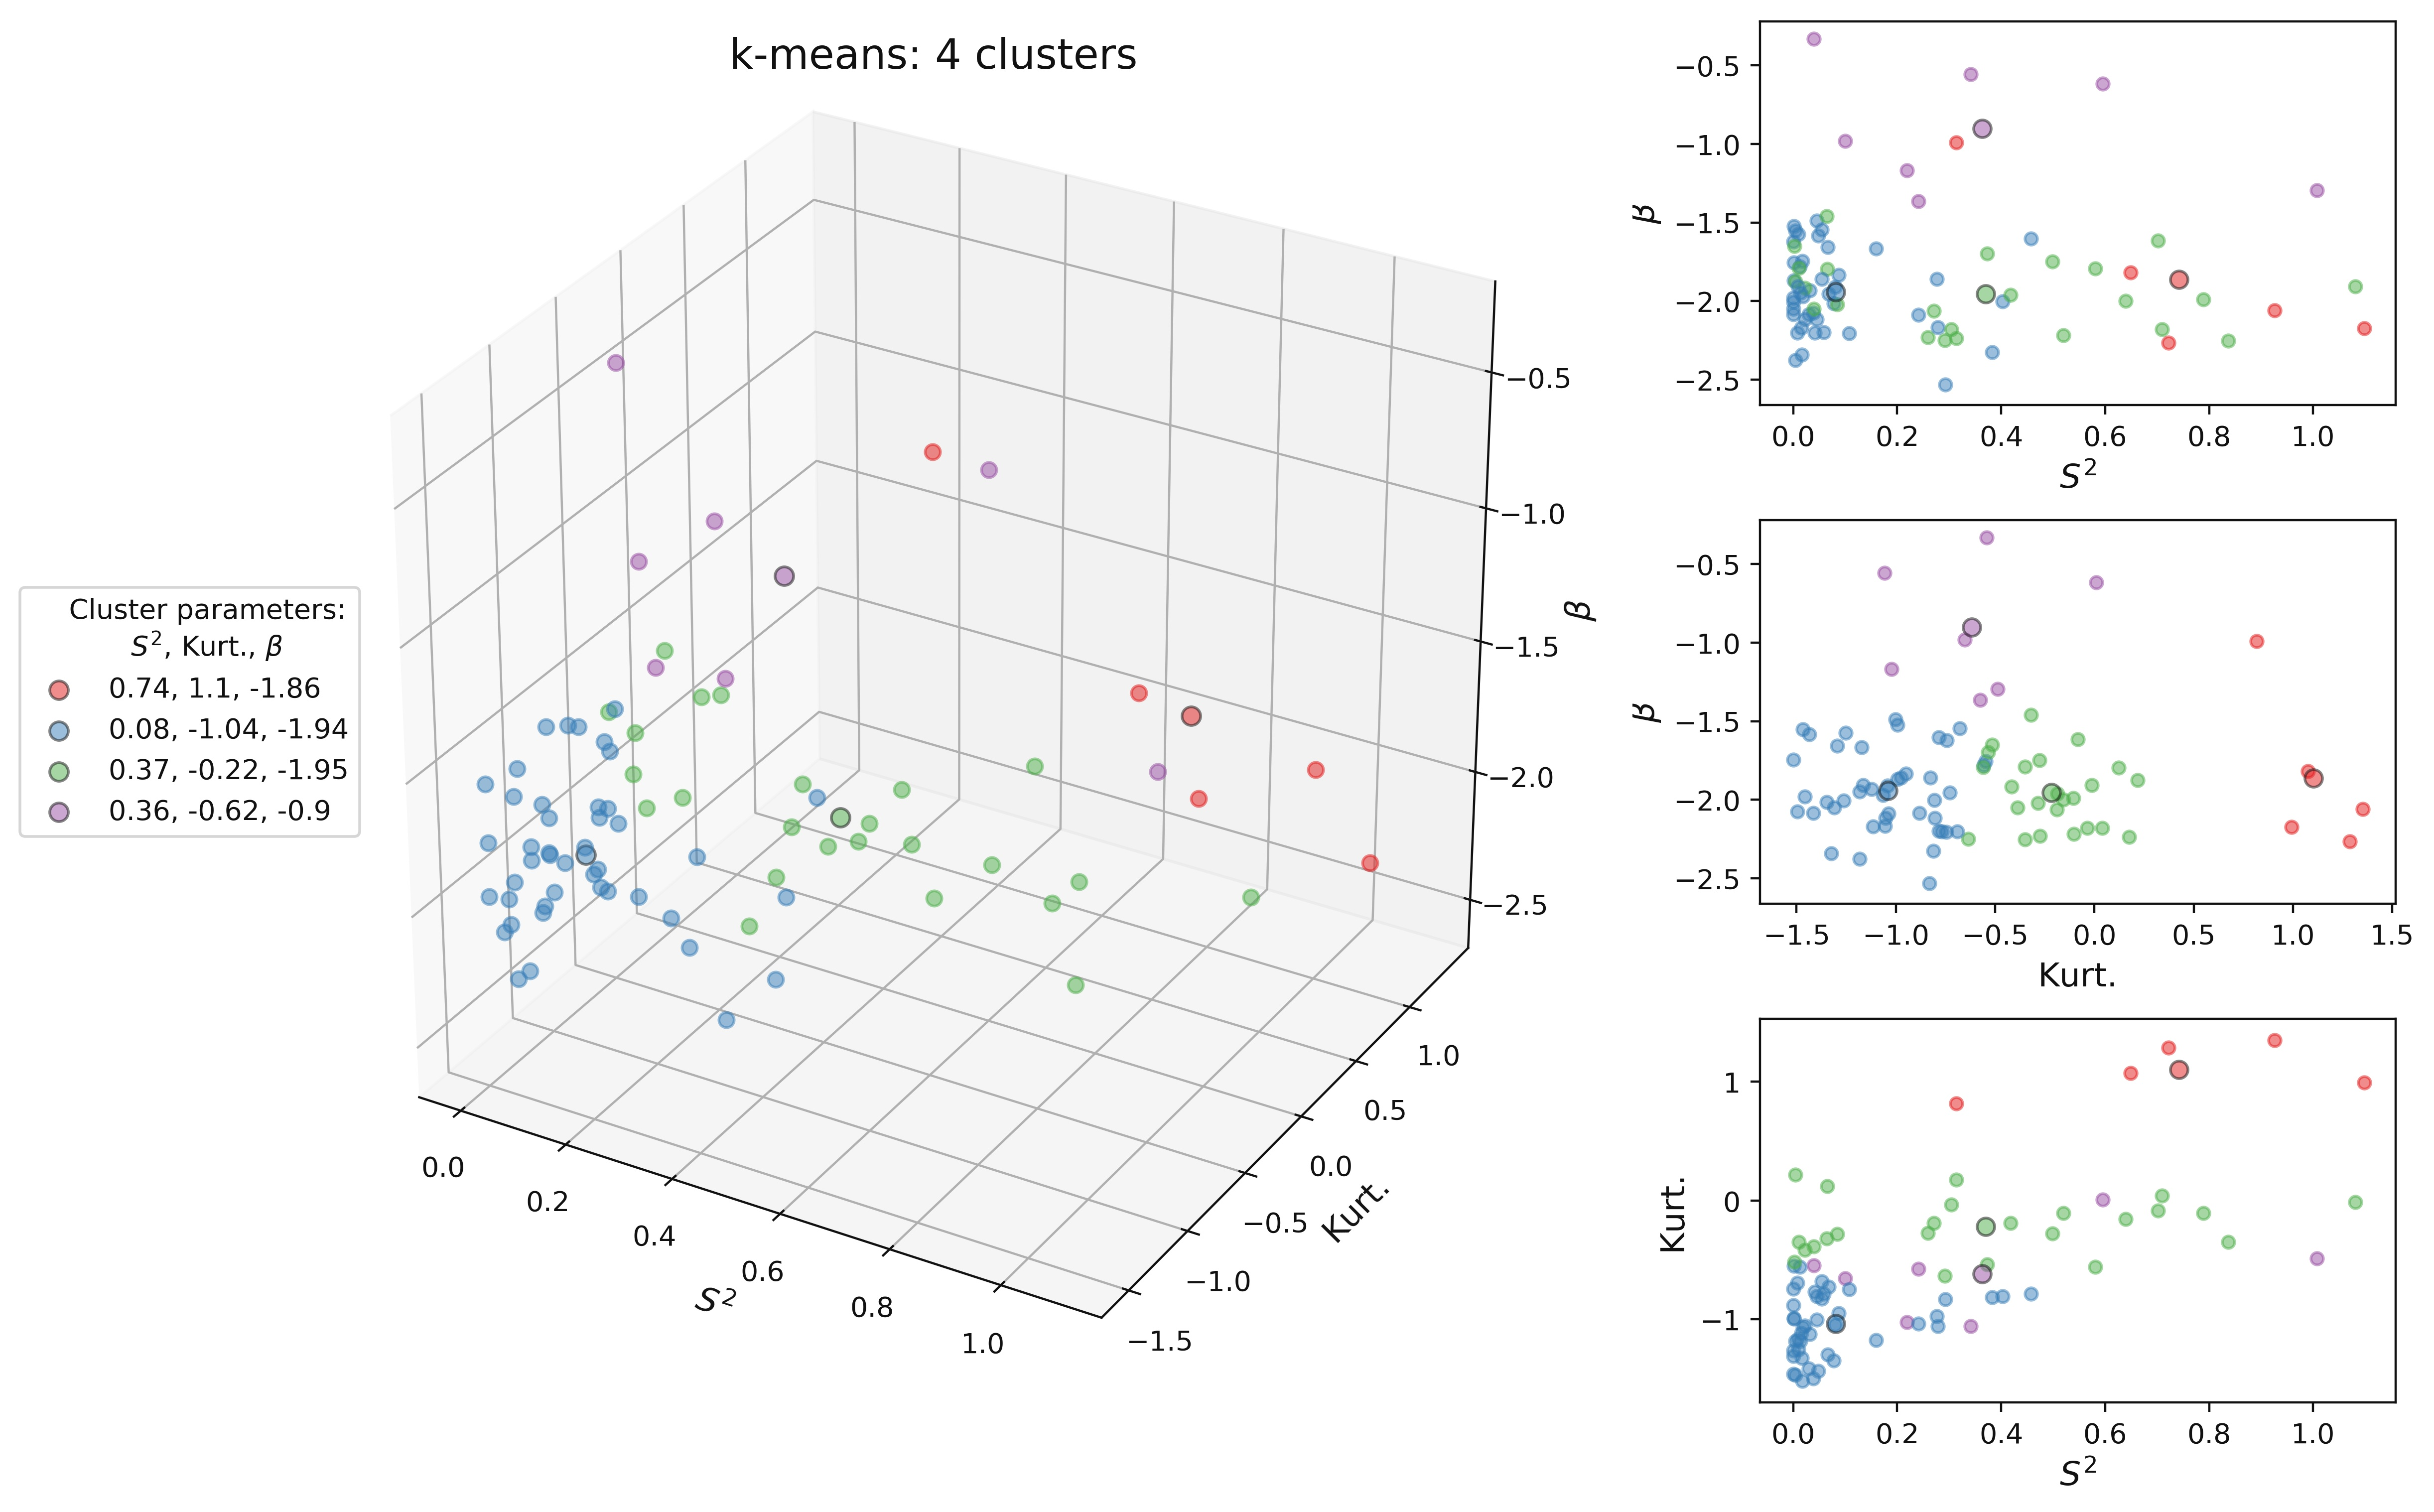
\includegraphics{Figuras/ex6/6_1/Exercicio6_1_grupo_noise_PSD_cluster_4.jpg}}		
	\end{center}
	\vspace{-3mm}	% acrescentar o espaçamento vertical apropriado entre a borda inferior da figura e a legenda ou a fonte quando não há legenda (o valor pode ser negativo para subir)
	\legenda{Figura 6.1.3: Técnica kmeans no espaço de parâmetros skewness$^{2}$ x kurtosis x $\beta$ para toda a família noise, cujo melhor resultado foi $n\_c$ = 4 (quatro clusters).}	% legenda - para deixar sem legenda usar comando \legenda{} (nunca deve-se comentar o comando \legenda)
	\label{ex6_fig3}
	%\FONTE{}	% fonte consultada (elemento obrigatório, mesmo que seja produção do próprio autor)
\end{figure}

Segundo resultado do agrupamento kmeans do grupo noise (usando $\alpha$):

\begin{figure}[ht!]
	%\caption{Série e histogramas.}
	\vspace{-3mm}	% acrescentar o espaçamento vertical apropriado entre o título e a borda superior da figura
	\begin{center}
		\resizebox{14cm}{!}{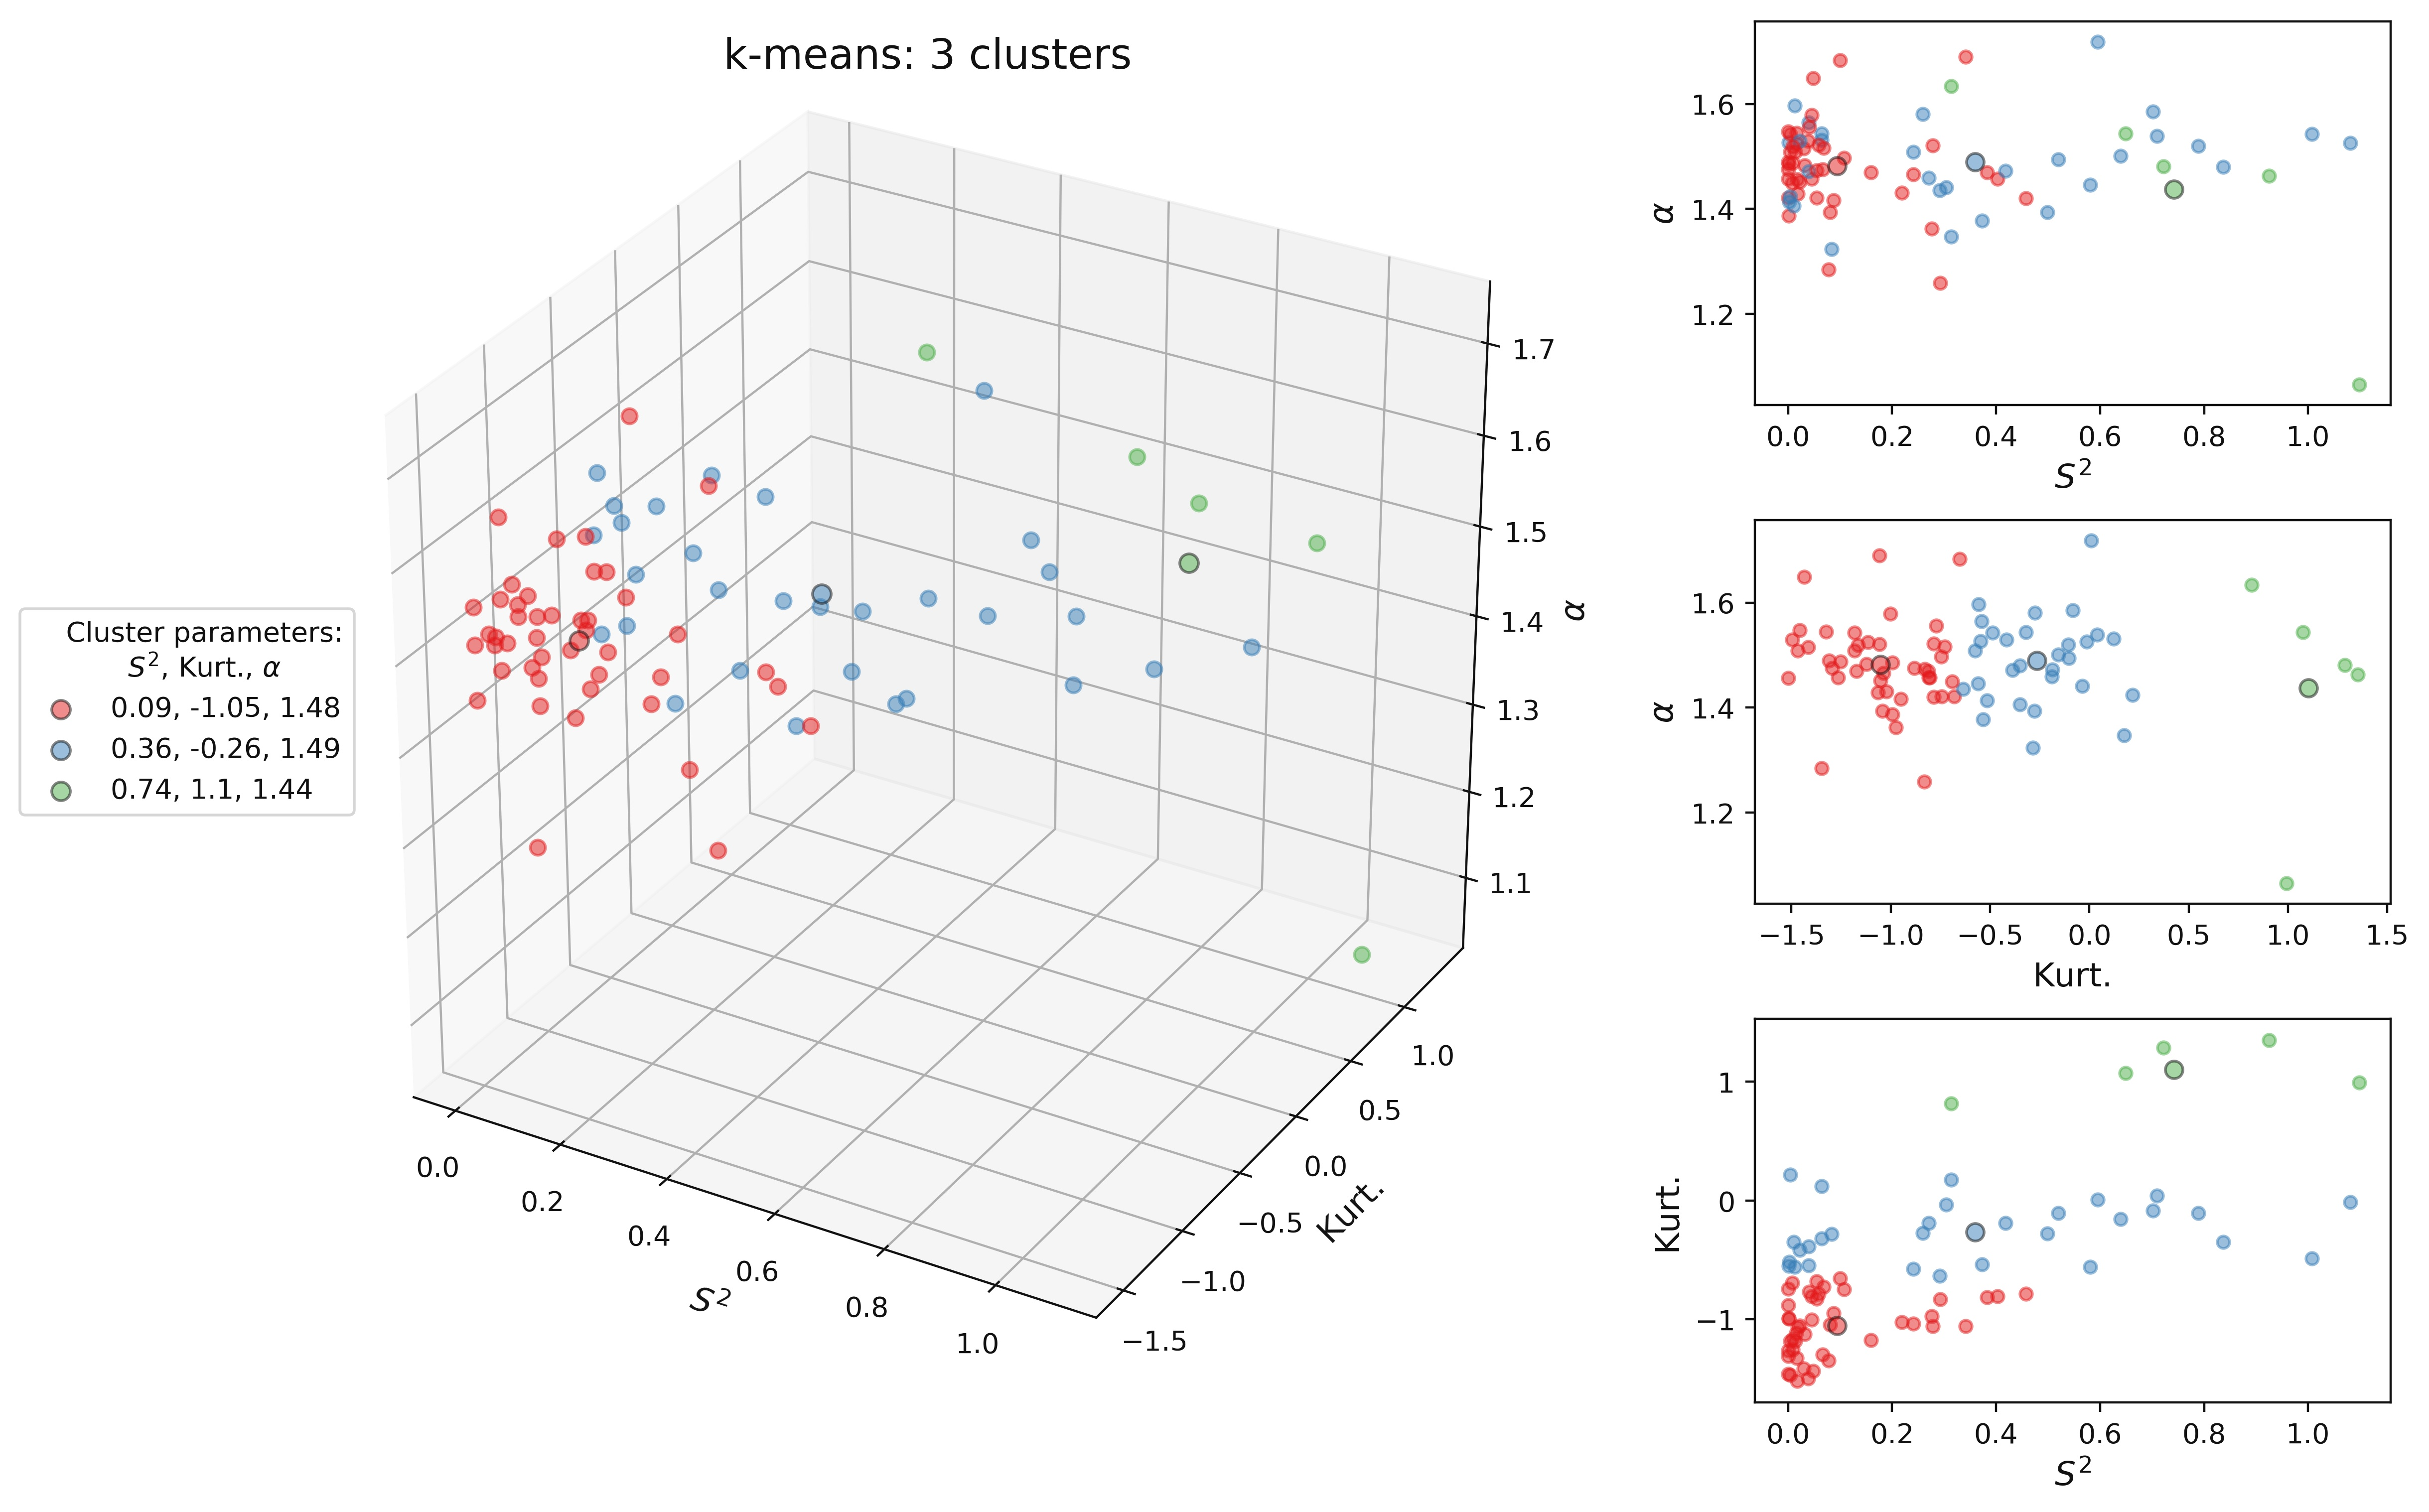
\includegraphics{Figuras/ex6/6_1/Exercicio6_1_grupo_noise_DFA_cluster_3.jpg}}		
	\end{center}
	\vspace{-3mm}	% acrescentar o espaçamento vertical apropriado entre a borda inferior da figura e a legenda ou a fonte quando não há legenda (o valor pode ser negativo para subir)
	\legenda{Figura 6.1.4: Técnica kmeans no espaço de parâmetros skewness$^{2}$ x kurtosis x $\alpha$ para toda a família noise, cujo melhor resultado foi $n\_c$ = 3 (três clusters).}	% legenda - para deixar sem legenda usar comando \legenda{} (nunca deve-se comentar o comando \legenda)
	\label{ex6_fig3}
	%\FONTE{}	% fonte consultada (elemento obrigatório, mesmo que seja produção do próprio autor)
\end{figure}

%%%%%%%%%%%%%%%%% Extra! %%%%%%%%%%%%%%%%%%%%%%%

\clearpage
Importante ressaltar que as análises espectrais do grupo colornoise foram consistentes com as cores de cada ruído ($\beta$ = 0, 1 e 2). A seguir está um plot da análise para $\beta$ = 1 (Figura 6.1.5). Por outro lado, a análise espectral do grupo chaosnoise apresentou índice espectral com faixa dinâmica extremamente ''lisa'', similar a um ruído branco. Isso ocorre pois as séries do grupo chaosnoise, como o mapeamento Logístico (Figura 6.1.6), pertencem a regimes antipersistentes. 

\begin{figure}[ht!]
	%\caption{Série e histogramas.}
	\vspace{-4mm}	% acrescentar o espaçamento vertical apropriado entre o título e a borda superior da figura
	\begin{center}
		\resizebox{12cm}{!}{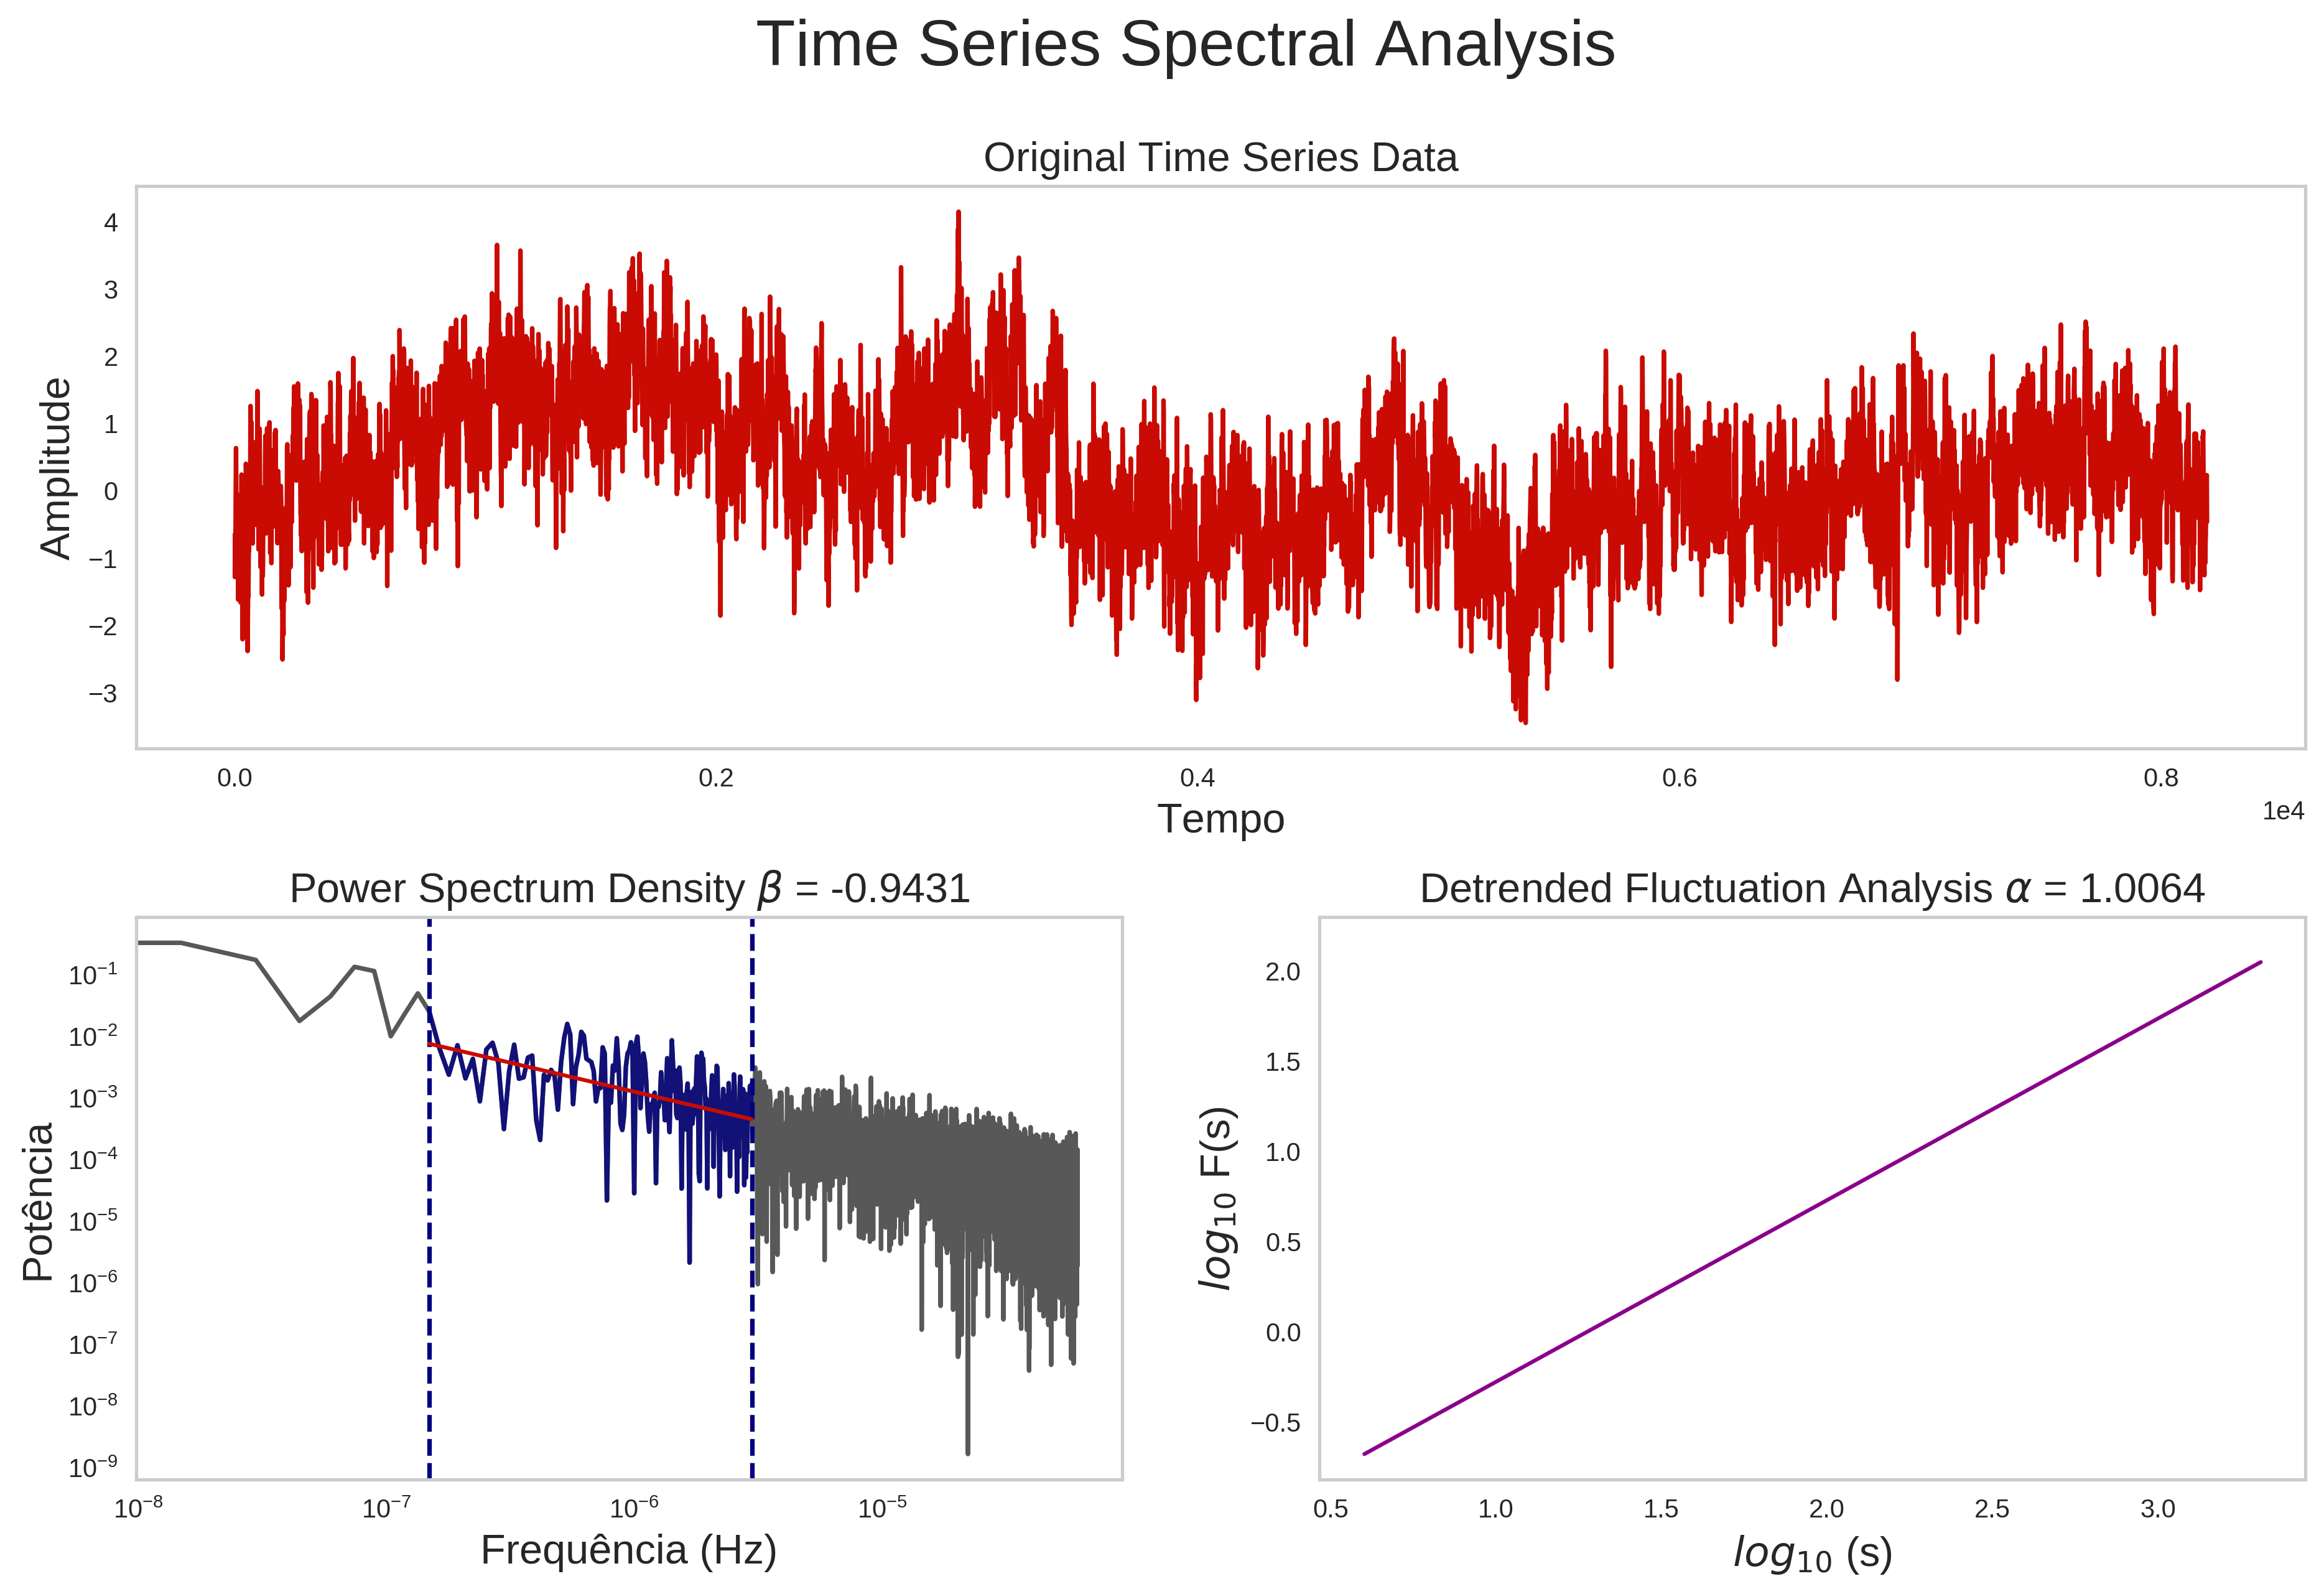
\includegraphics{Figuras/ex6/6_1/Exercicio6_1_grupo_colornoise_Specplus_betaNoise_1_ANALYSIS_PSD_DFA_2.png}}		
	\end{center}
	\vspace{-2mm}	% acrescentar o espaçamento vertical apropriado entre a borda inferior da figura e a legenda ou a fonte quando não há legenda (o valor pode ser negativo para subir)
	\legenda{Figura 6.1.5: Análise espectral do grupo colornoise para $\beta$ = 1.}	% legenda - para deixar sem legenda usar comando \legenda{} (nunca deve-se comentar o comando \legenda)
	\label{ex6_fig1}
	%\FONTE{}	% fonte consultada (elemento obrigatório, mesmo que seja produção do próprio autor)
\end{figure}

\begin{figure}[ht!]
	%\caption{Série e histogramas.}
	\vspace{-4mm}	% acrescentar o espaçamento vertical apropriado entre o título e a borda superior da figura
	\begin{center}
		\resizebox{12cm}{!}{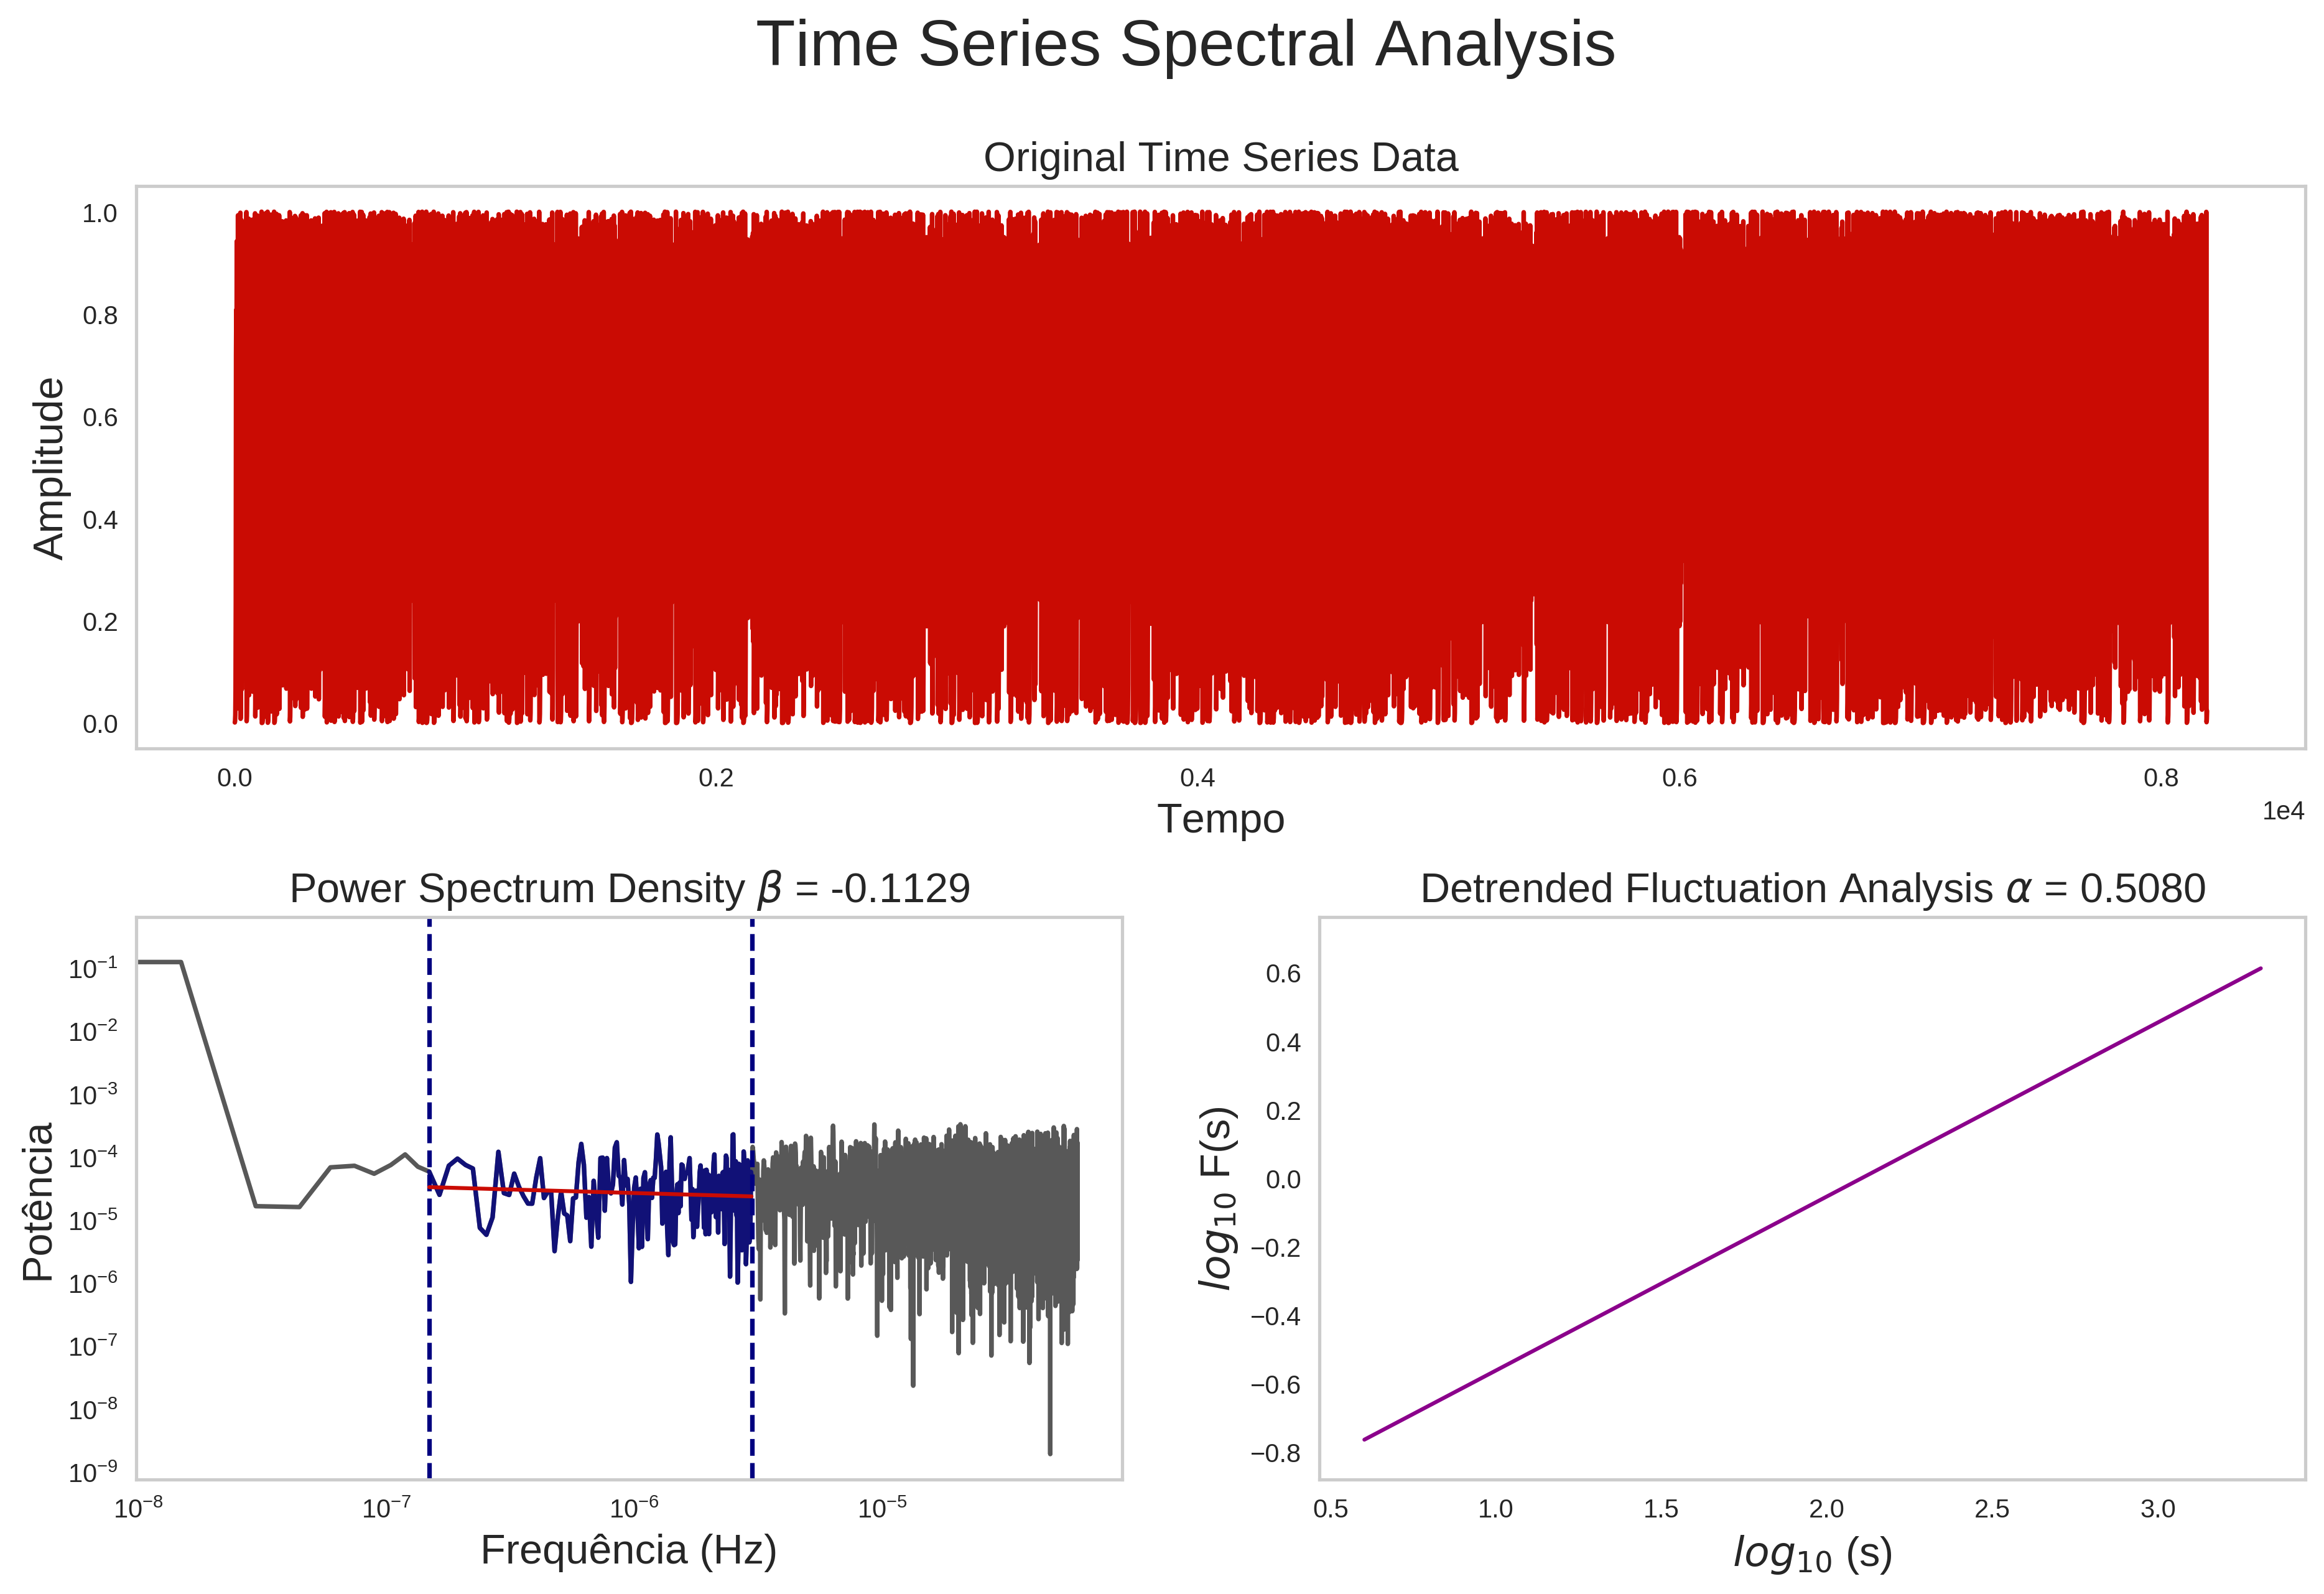
\includegraphics{Figuras/ex6/6_1/Exercicio6_1_Logistico_Specplus_rho_4.0_ANALYSIS_PSD_DFA_2.png}}		
	\end{center}
	\vspace{-2mm}	% acrescentar o espaçamento vertical apropriado entre a borda inferior da figura e a legenda ou a fonte quando não há legenda (o valor pode ser negativo para subir)
	\legenda{Figura 6.1.6: Análise espectral do grupo chaosnoise para o mapeamento Logístico com $\rho$ = 4.}	% legenda - para deixar sem legenda usar comando \legenda{} (nunca deve-se comentar o comando \legenda)
	\label{ex6_fig1}
	%\FONTE{}	% fonte consultada (elemento obrigatório, mesmo que seja produção do próprio autor)
\end{figure}

%%%%%%%%%%%%%%%%%%%%%%%%%%%%%%%%%%%%5 6.2 %%%%%%%%%%%%%%%%%%%%%%%%%%%%%%%%%%%%%%%%%%%%%
\clearpage
\subsection*{6.2}
\addcontentsline{toc}{section}{\protect\numberline{} 6.2}%

%Os plots a seguir exemplificam a análise realizada. 
Para este exercício foi utilizado o script kmeans\_3D\_plus\_data.py. Os resultados de cada família estão em suas respectivas pastas dentro da pasta referente a este exercício - \textbf{6.2}. As séries temporais \textit{ST-Sol3GHz} e \textit{ST-surftemp504} foram importadas da pasta \textbf{time\_series\_data}. A \textit{ST-OWS\_NDC\_Covid19} é referente ao Brasil e foi baixada na execução do código. 

Os plots a seguir foram escolhidos por exibir os resultados mais interessantes. Cada família está identificada com a cor vermelha (representando um cluster único, ou seja, $n\_c$ = 1) e as séries temporais acima citadas são plotadas no mesmo espaço de parâmetros. Com isso pode-se identificar como as séries temporais se posicionam nos espaços considerados com relação aos sinais presentes na tabela \textit{Dataset\_signal}. De todas as famílias, apenas chaosnoise não permitiu identificar alguma das três séries temporais como pertencente ao cluster da família. Para o grupo noise (Figura 6.2.1), a série \textit{ST-surftemp504} esteve próxima dos sinais da família no espaço skewness$^{2}$ x kurtosis x $\beta$, mas nenhuma série temporal exibiu o mesmo comportamento no espaço skewness$^{2}$ x kurtosis x $\alpha$. Para os grupos colornoise (Figura 6.2.2) e pmnoise (Figura 6.2.3), o comportamento das séries temporais com relação aos sinais foi basicamente o mesmo para ambos os espaços de parâmetros considerados.

\begin{figure}[ht!]
	%\caption{Série e histogramas.}
	\vspace{0mm}	% acrescentar o espaçamento vertical apropriado entre o título e a borda superior da figura
	\begin{center}
		\resizebox{14cm}{!}{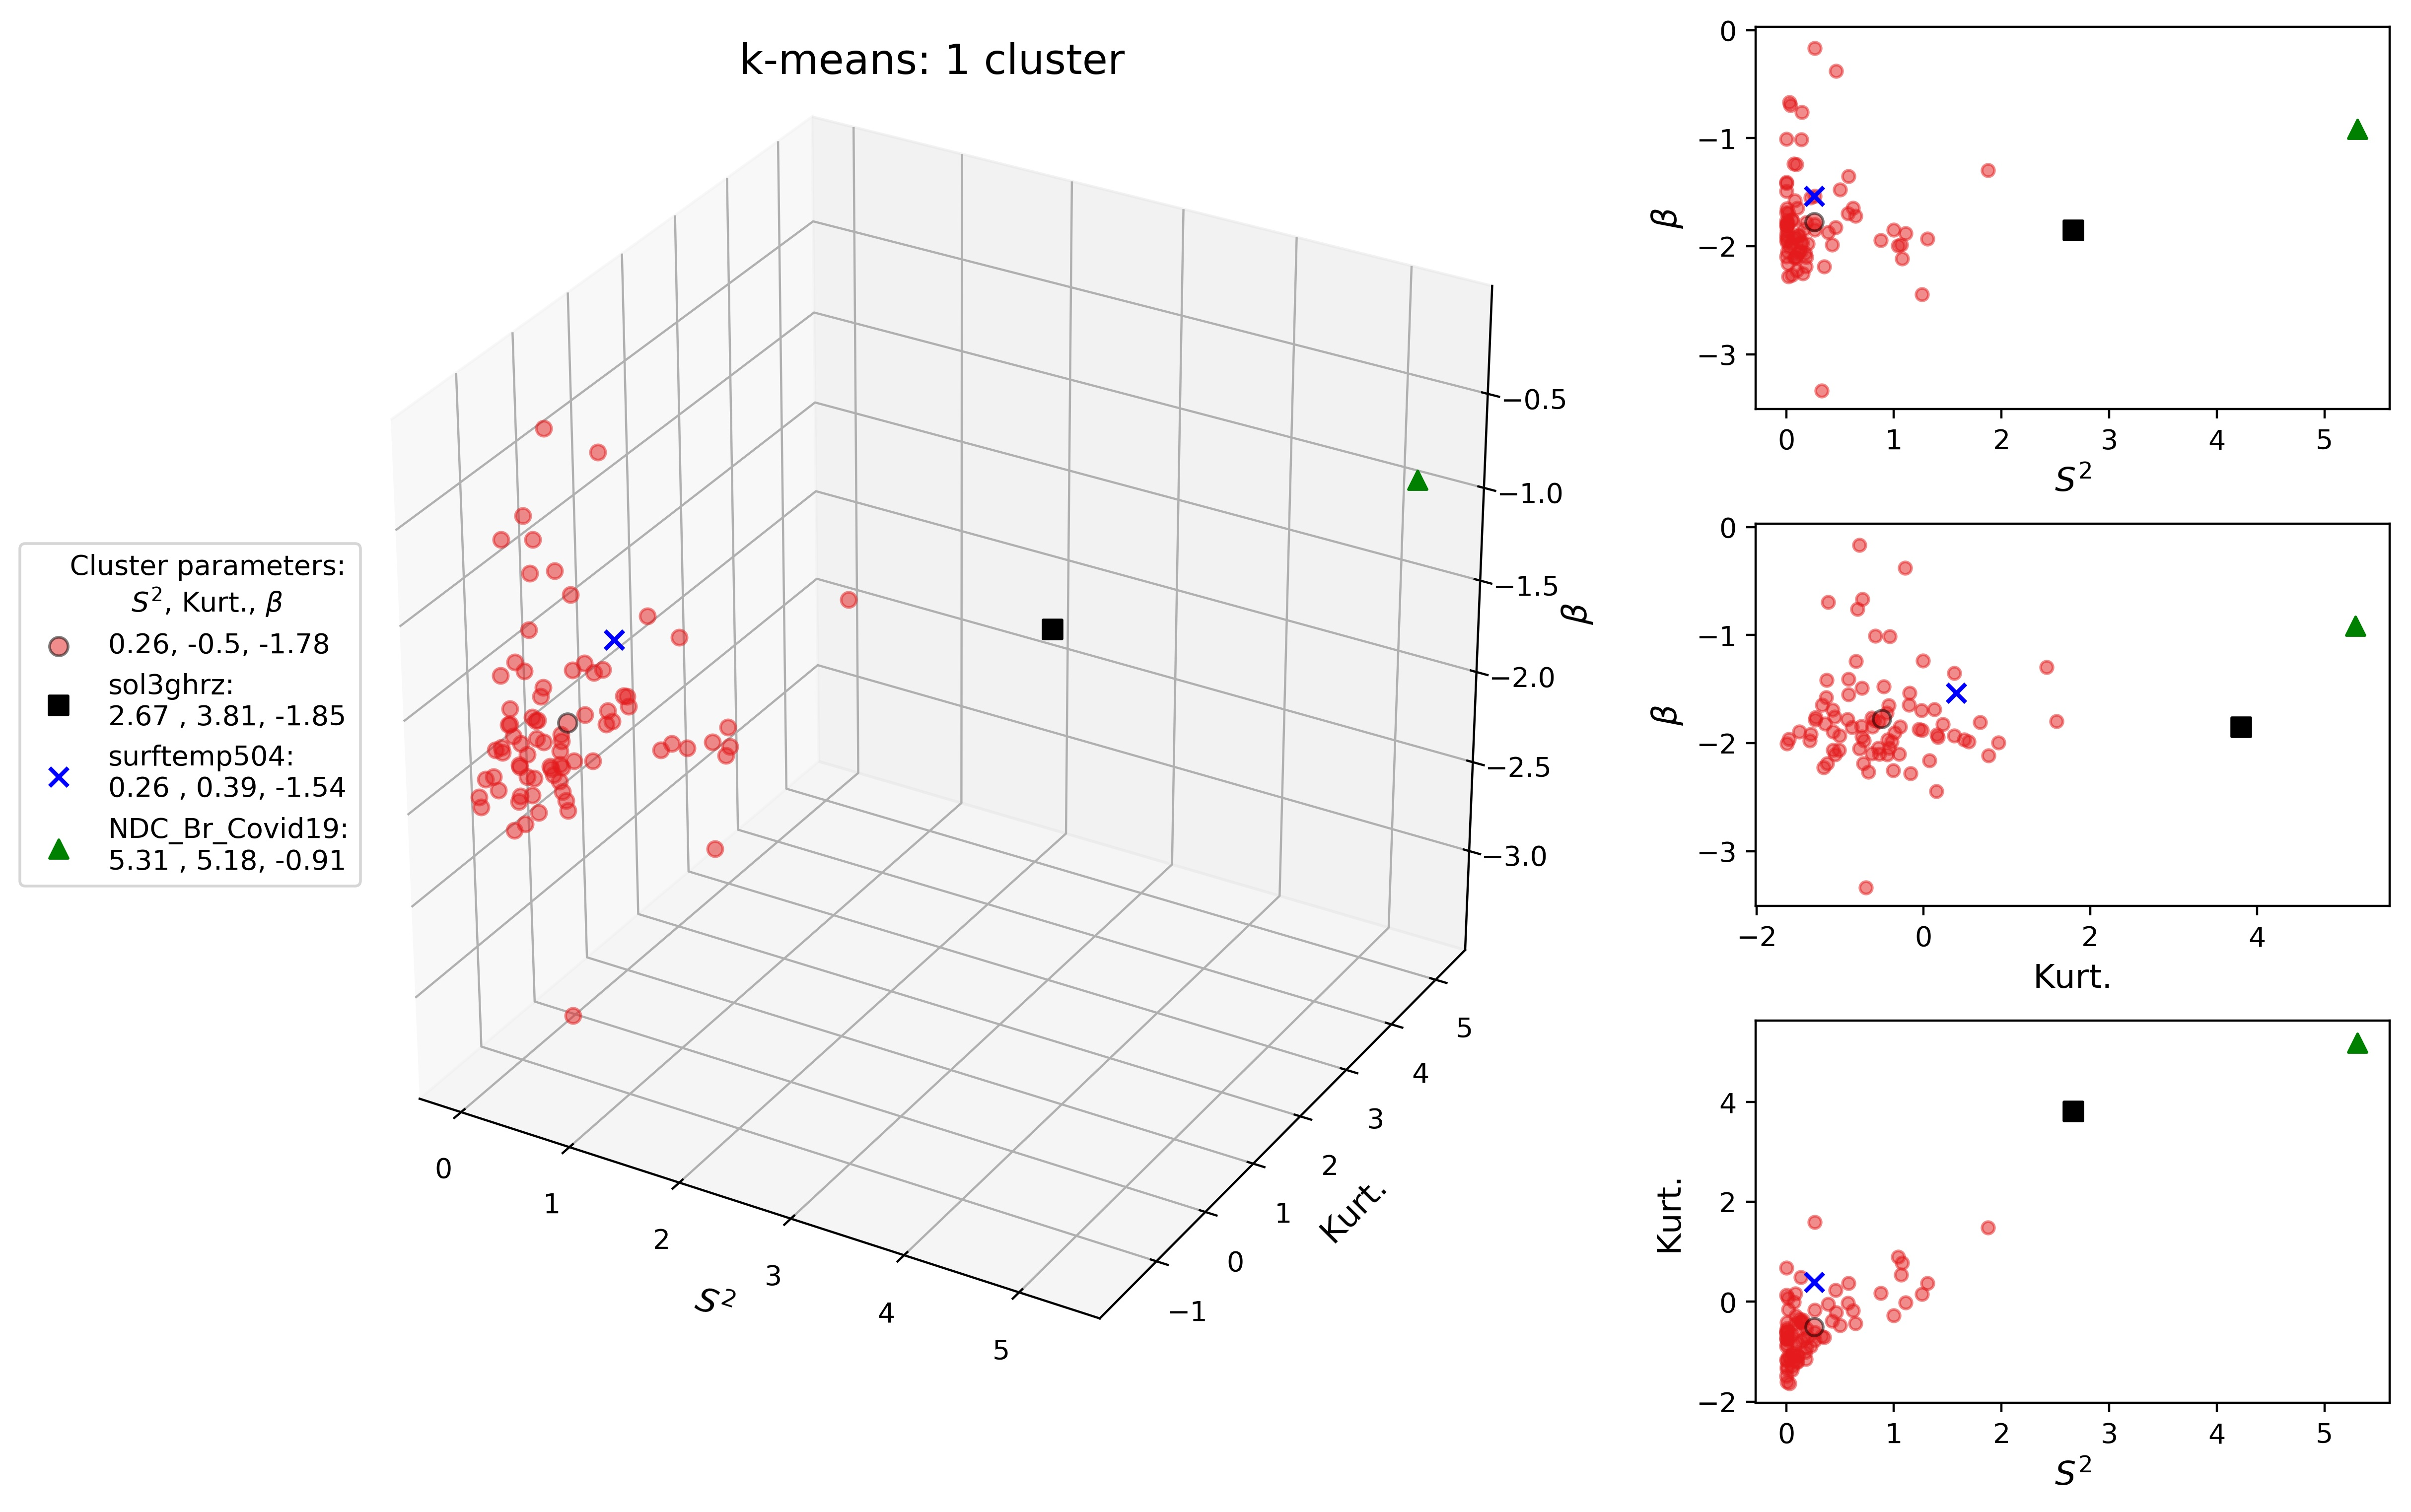
\includegraphics{Figuras/ex6/6_2/Exercicio6_2_grupo_noise_PSD_cluster_1.jpg}}		
	\end{center}
	\vspace{-2mm}	% acrescentar o espaçamento vertical apropriado entre a borda inferior da figura e a legenda ou a fonte quando não há legenda (o valor pode ser negativo para subir)
	\legenda{Figura 6.2.1: Espaço skewness$^{2}$ x kurtosis x $\beta$ do grupo noise e a posição relativa das três séries temporais deste exercício. A série \textit{ST-surftemp504} foi a que mais se aproximou dos sinais deste grupo.}	% legenda - para deixar sem legenda usar comando \legenda{} (nunca deve-se comentar o comando \legenda)
	\label{ex6_fig3}
	%\FONTE{}	% fonte consultada (elemento obrigatório, mesmo que seja produção do próprio autor)
\end{figure}

\begin{figure}[ht!]
	%\caption{Série e histogramas.}
	\vspace{0mm}	% acrescentar o espaçamento vertical apropriado entre o título e a borda superior da figura
	\begin{center}
		\resizebox{14cm}{!}{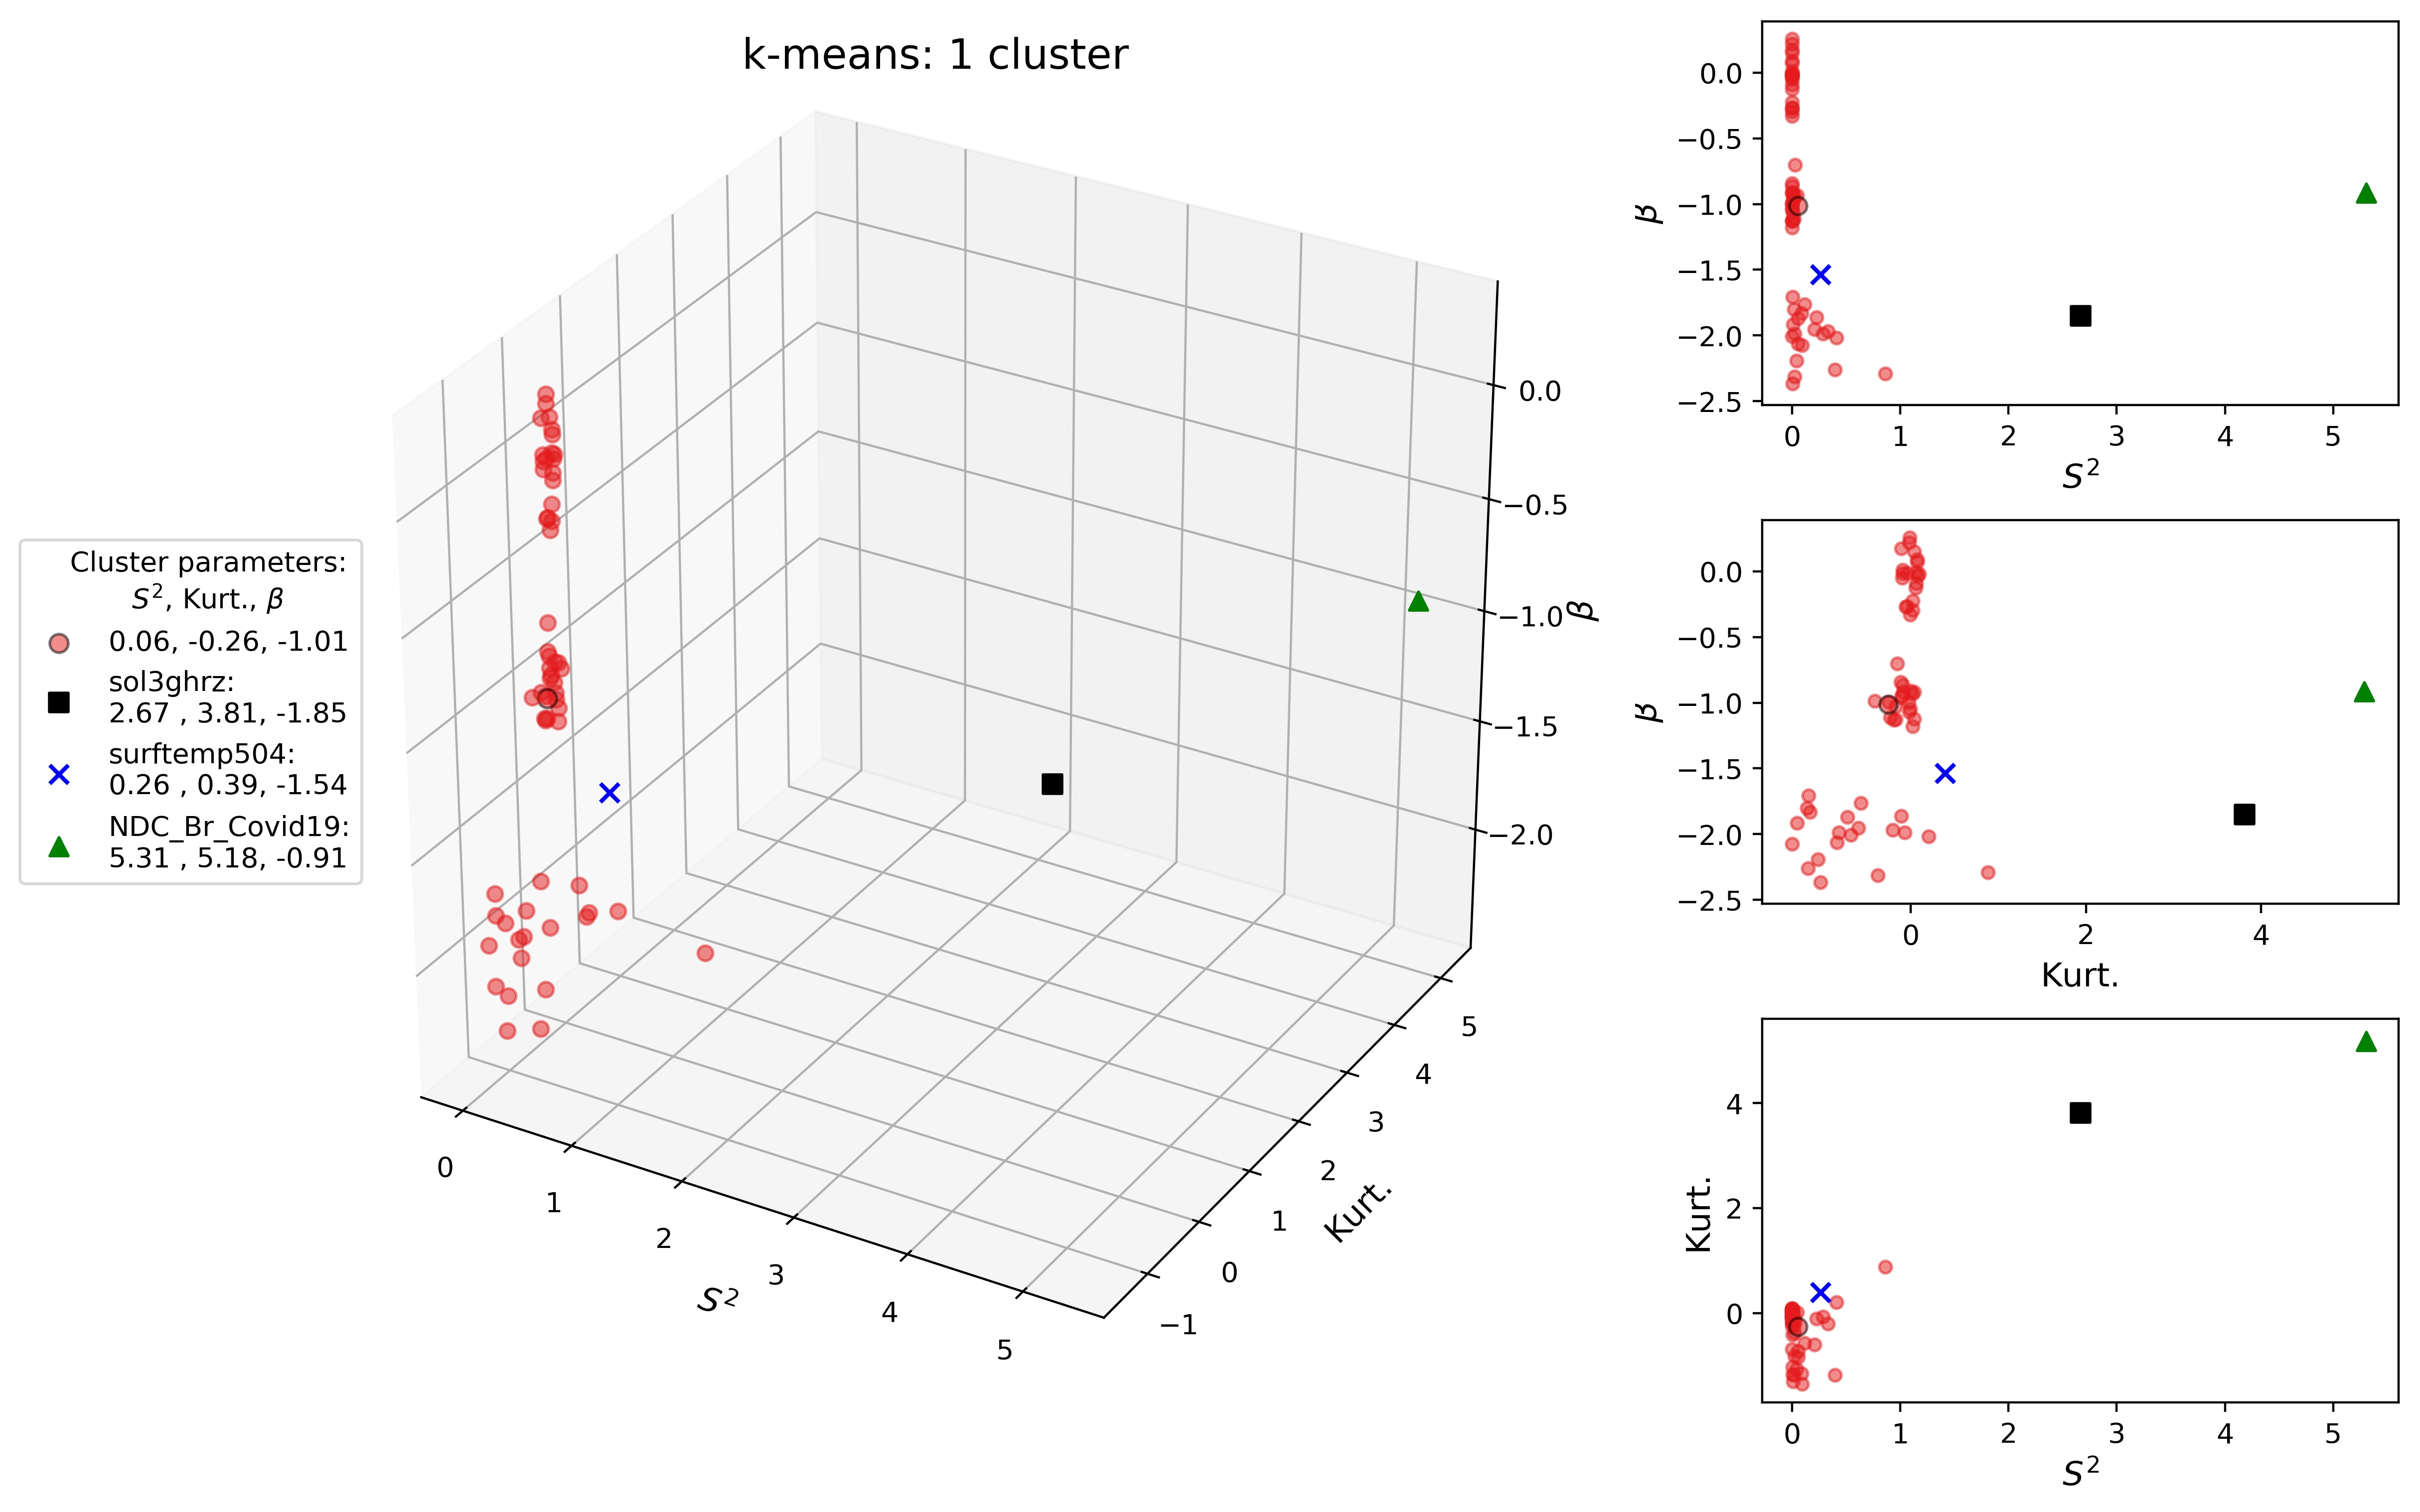
\includegraphics{Figuras/ex6/6_2/Exercicio6_2_grupo_colornoise_PSD_cluster_1.jpg}}		
	\end{center}
	\vspace{-2mm}	% acrescentar o espaçamento vertical apropriado entre a borda inferior da figura e a legenda ou a fonte quando não há legenda (o valor pode ser negativo para subir)
	\legenda{Figura 6.2.2: Espaço skewness$^{2}$ x kurtosis x $\beta$ do grupo colornoise e a posição relativa das três séries temporais deste exercício. A série \textit{ST-surftemp504} foi a que mais se aproximou dos sinais deste grupo.}	% legenda - para deixar sem legenda usar comando \legenda{} (nunca deve-se comentar o comando \legenda)
	\label{ex6_fig3}
	%\FONTE{}	% fonte consultada (elemento obrigatório, mesmo que seja produção do próprio autor)
\end{figure}

\begin{figure}[ht!]
	%\caption{Série e histogramas.}
	\vspace{0mm}	% acrescentar o espaçamento vertical apropriado entre o título e a borda superior da figura
	\begin{center}
		\resizebox{14cm}{!}{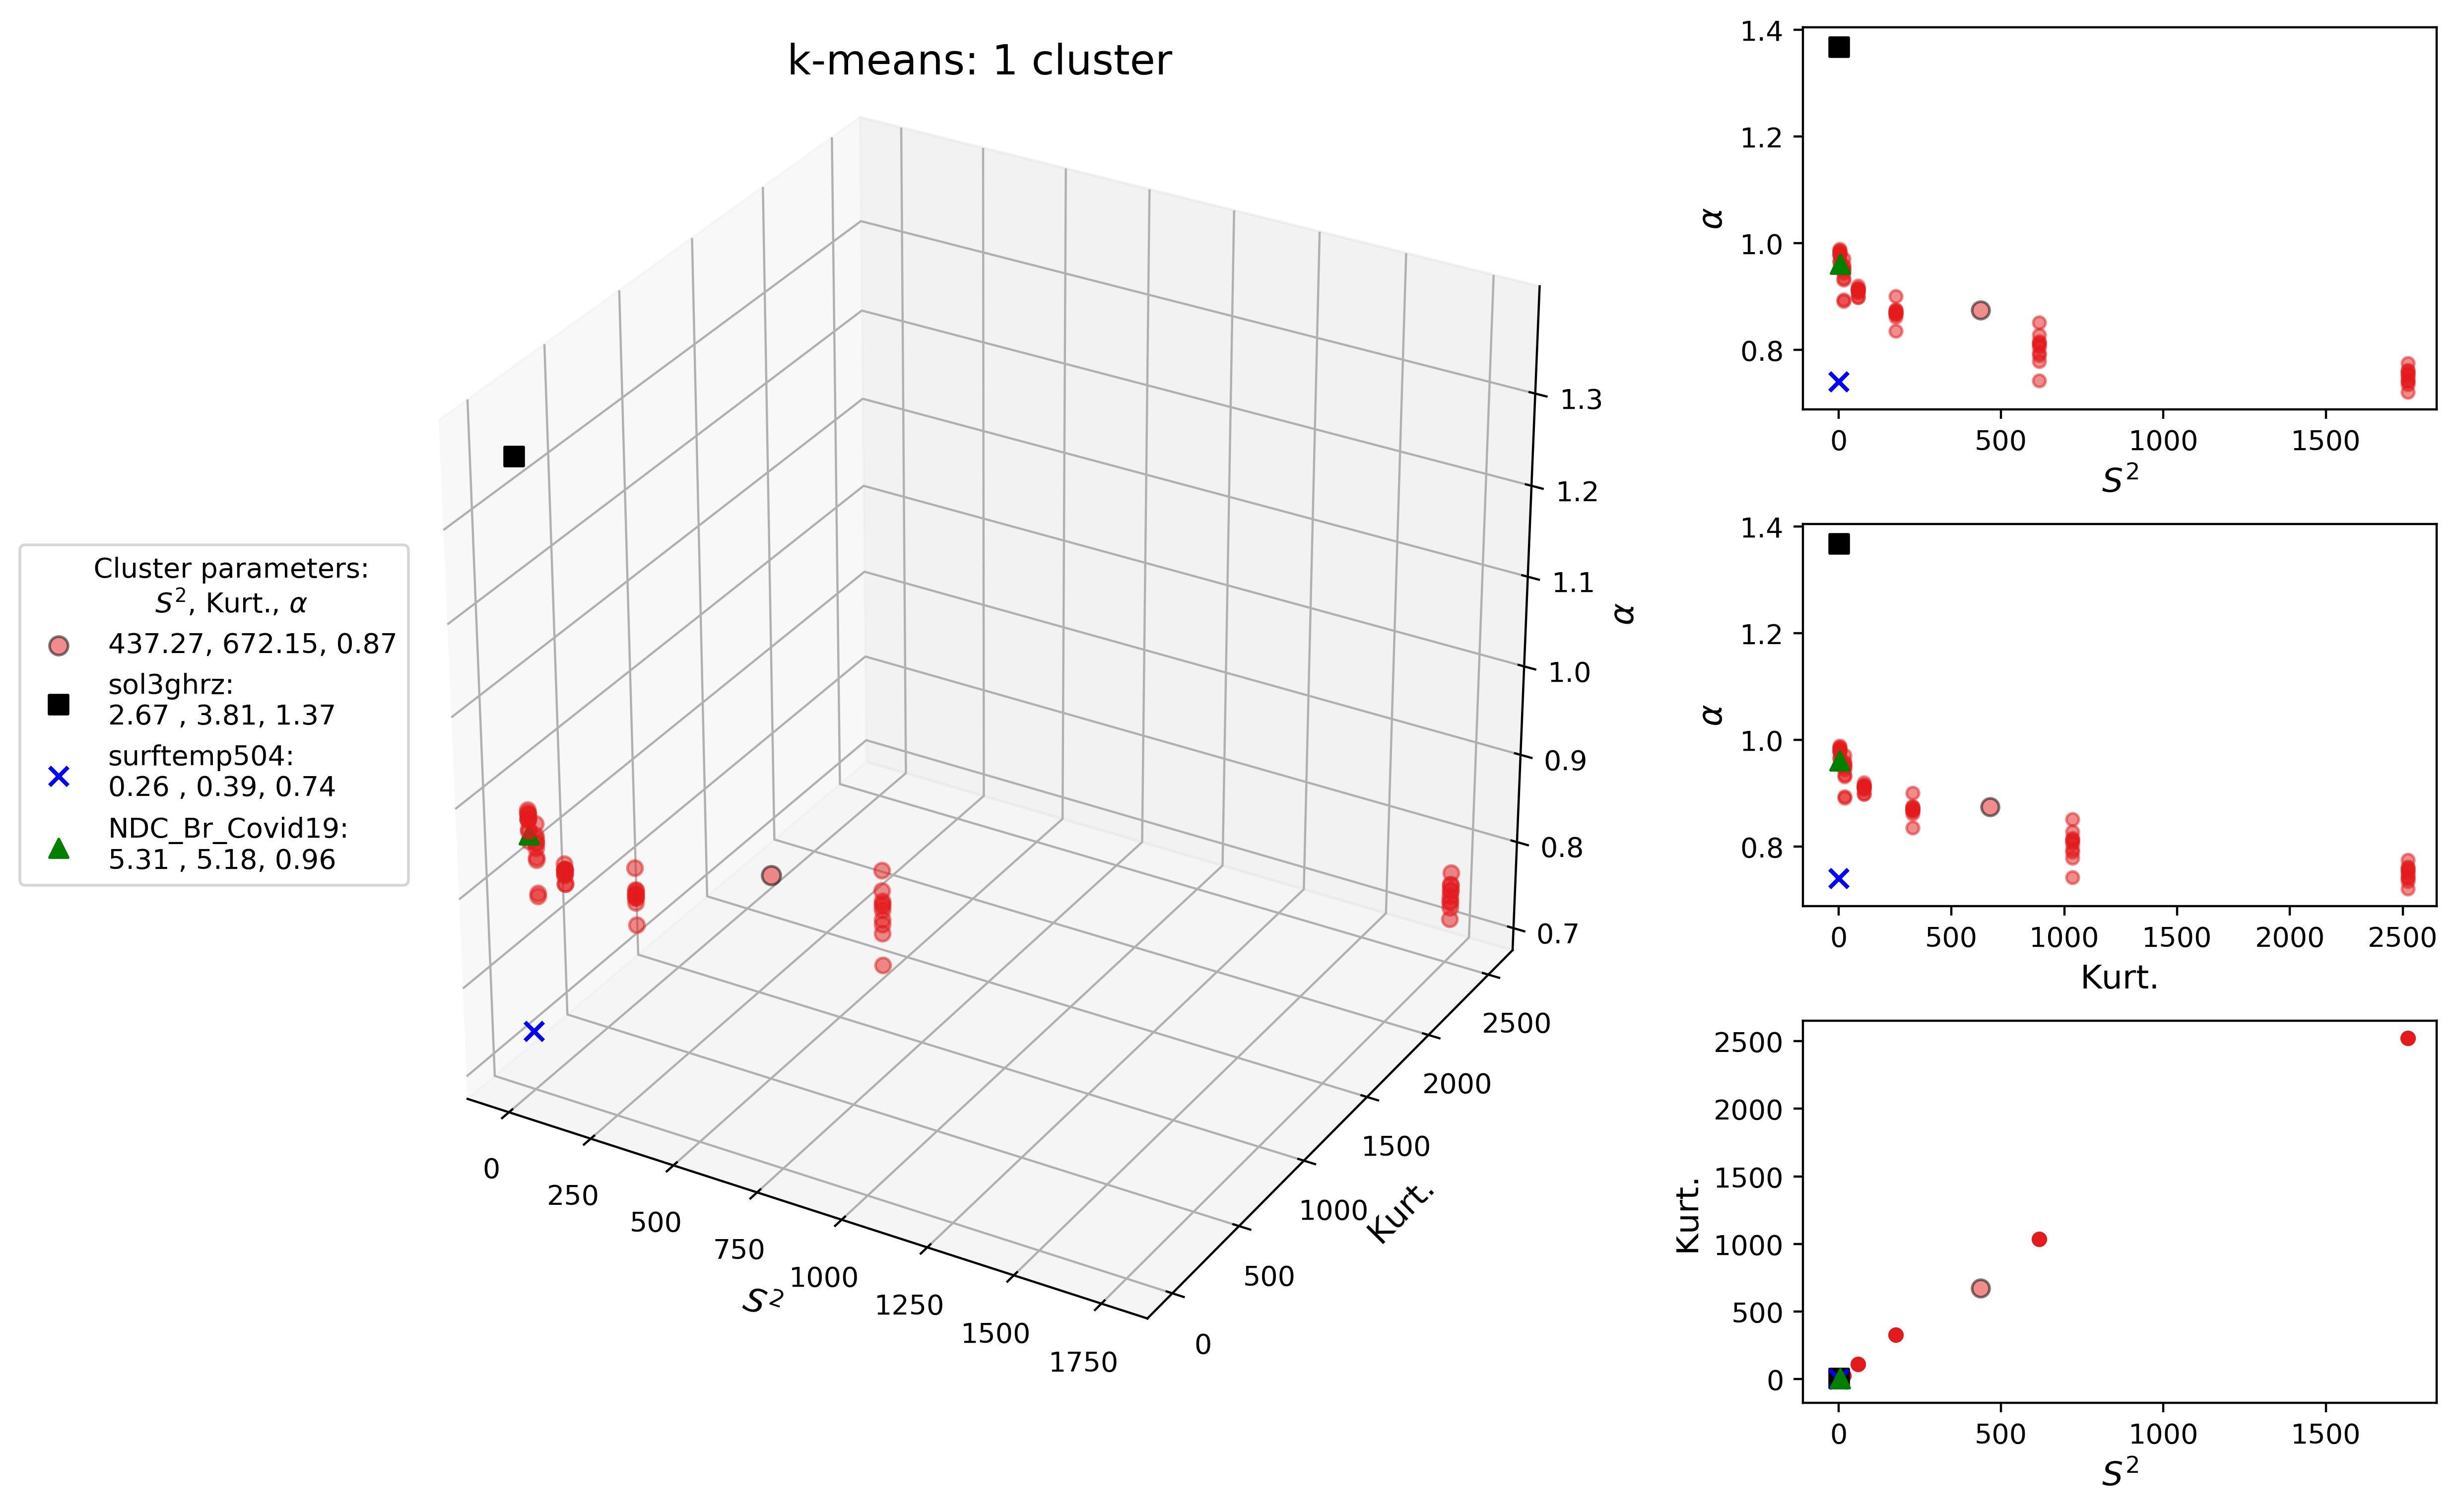
\includegraphics{Figuras/ex6/6_2/Exercicio6_2_grupo_pmnoise_DFA_cluster_1.jpg}}		
	\end{center}
	\vspace{-2mm}	% acrescentar o espaçamento vertical apropriado entre a borda inferior da figura e a legenda ou a fonte quando não há legenda (o valor pode ser negativo para subir)
	\legenda{Figura 6.2.3: Espaço skewness$^{2}$ x kurtosis x $\alpha$ do grupo pmnoise e a posição relativa das três séries temporais deste exercício. A série \textit{NDC\_Br\_Covid19} foi a que mais se aproximou dos sinais deste grupo.}	% legenda - para deixar sem legenda usar comando \legenda{} (nunca deve-se comentar o comando \legenda)
	\label{ex6_fig3}
	%\FONTE{}	% fonte consultada (elemento obrigatório, mesmo que seja produção do próprio autor)
\end{figure}

%%%%%%%%%%%%%%%%%%%%%%%%%%%%%%%%%%%%%%% 6.3 %%%%%%%%%%%%%%%%%%%%%%%%%%%%%%%5%%
\clearpage
\subsection*{6.3}
\addcontentsline{toc}{section}{\protect\numberline{} 6.3}%

Os dois plots a seguir resultam da análise da série \textit{ST-OWS\_NDC\_Covid19} para todos os países. O número de clusters ideal foi selecionado de acordo com o método do cotovelo, e foi de três para os dois espaços de parâmetros deste exercício. O algoritmo utilizado foi o kmeans\_2D\_group\_flags.py, que agrupou cada país em seu respectivo cluster em arquivos .csv (identificados pelo centróide do grupo). Estes arquivos e demais plots se encontram na pasta deste exercício - \textbf{6.3}. 

\begin{figure}[ht!]
	%\caption{Série e histogramas.}
	\vspace{0mm}	% acrescentar o espaçamento vertical apropriado entre o título e a borda superior da figura
	\begin{center}
		\resizebox{15cm}{!}{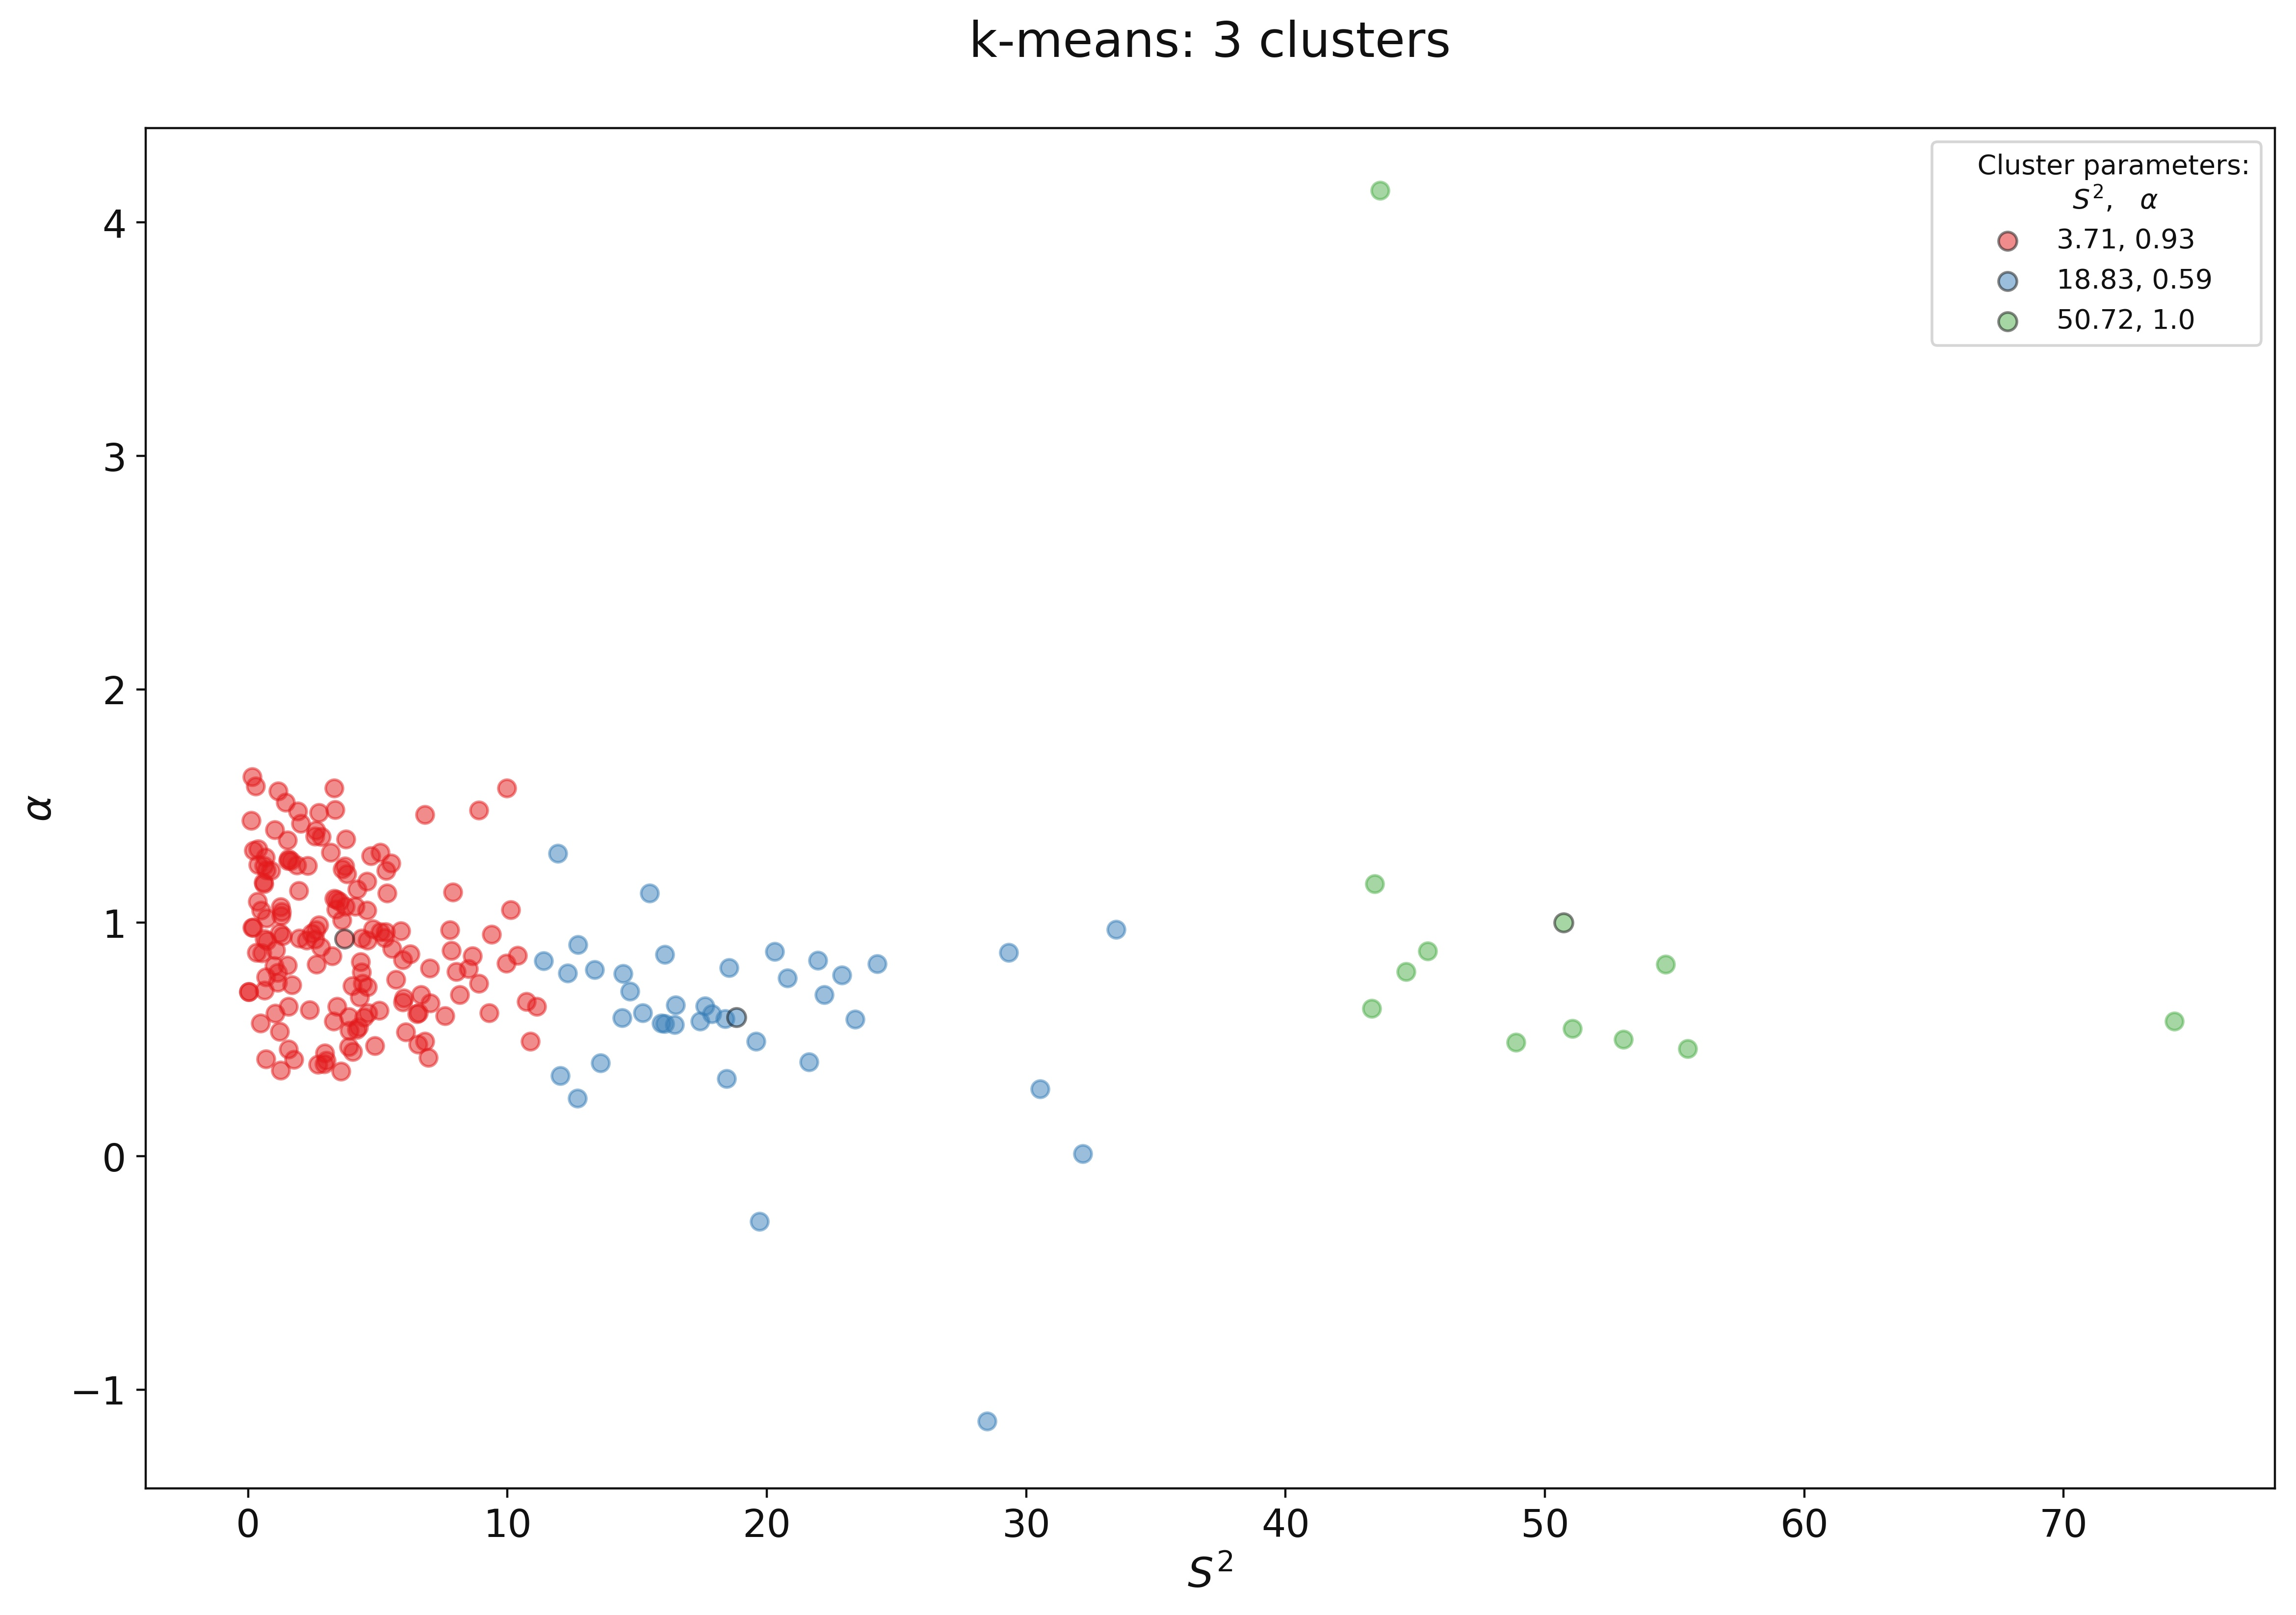
\includegraphics{Figuras/ex6/6_3/Exercicio6_3_S2vsAlfa_cluster_3.jpg}}		
	\end{center}
	\vspace{-2mm}	% acrescentar o espaçamento vertical apropriado entre a borda inferior da figura e a legenda ou a fonte quando não há legenda (o valor pode ser negativo para subir)
	\legenda{Figura 6.3.1: Resultado do agrupamento do número de casos diários de Covid19 para todos os países no espaço S$^{2}$ $\times$ $\alpha$.}	% legenda - para deixar sem legenda usar comando \legenda{} (nunca deve-se comentar o comando \legenda)
	\label{ex6_fig3}
	%\FONTE{}	% fonte consultada (elemento obrigatório, mesmo que seja produção do próprio autor)
\end{figure}

Nese exercício, os grupos de países no espaço S$^{2}$ x $\alpha$ se encontram nos seguintes arquivos: \textit{Exercicio6\_3\_S2vsAlfa\_cluster\_0\_x\_3.67\_y\_0.93\_flags.csv} (cluster vemelho), \textit{Exercicio6\_3\_S2vsAlfa\_cluster\_1\_x\_18.64\_y\_0.66\_flags.csv} (cluster azul) e \textit{Exercicio6\_3\_S2vsAlfa\_cluster\_2\_x\_53.82\_y\_1.04\_flags.csv} (cluster verde).

\clearpage

\begin{figure}[ht!]
	%\caption{Série e histogramas.}
	\vspace{0mm}	% acrescentar o espaçamento vertical apropriado entre o título e a borda superior da figura
	\begin{center}
		\resizebox{15cm}{!}{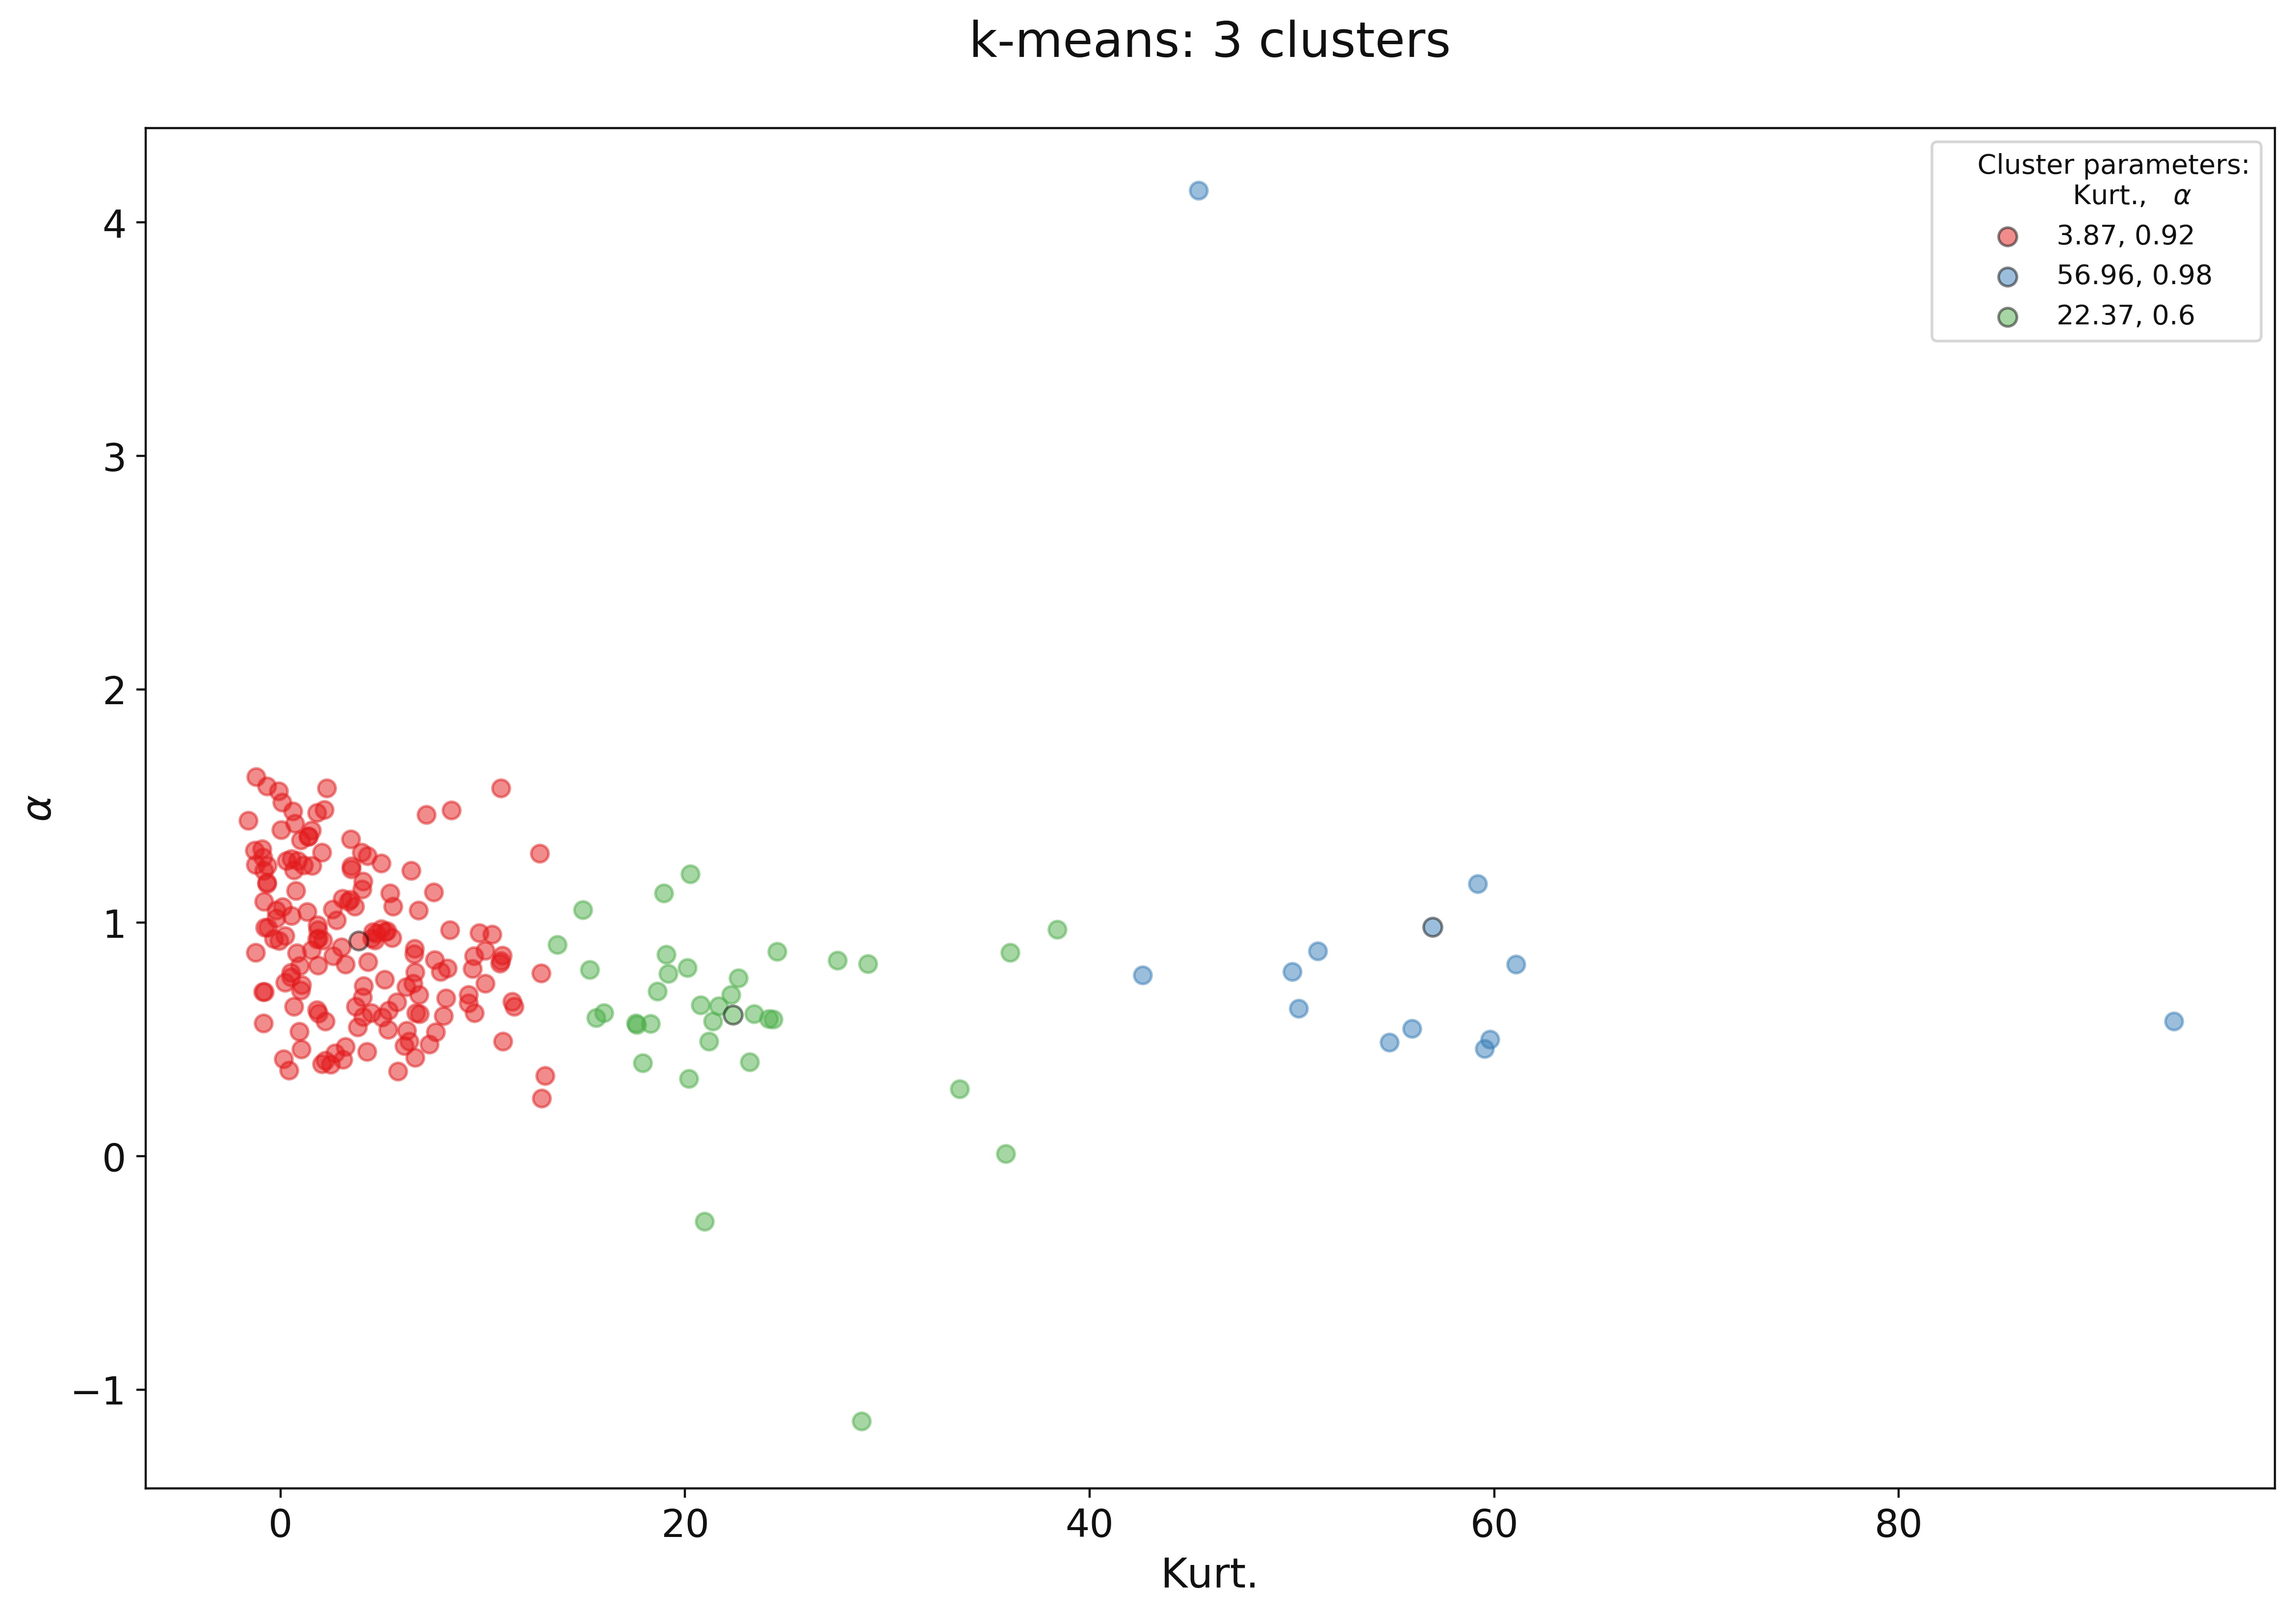
\includegraphics{Figuras/ex6/6_3/Exercicio6_3_KvsAlfa_cluster_3.jpg}}		
	\end{center}
	\vspace{-2mm}	% acrescentar o espaçamento vertical apropriado entre a borda inferior da figura e a legenda ou a fonte quando não há legenda (o valor pode ser negativo para subir)
	\legenda{Figura 6.3.2: Resultado do agrupamento do número de casos diários de Covid19 para todos os países no espaço K $\times$ $\alpha$.}	% legenda - para deixar sem legenda usar comando \legenda{} (nunca deve-se comentar o comando \legenda)
	\label{ex6_fig3}
	%\FONTE{}	% fonte consultada (elemento obrigatório, mesmo que seja produção do próprio autor)
\end{figure}

Nese exercício, os grupos de países no espaço K x $\alpha$ se encontram nos seguintes arquivos: \textit{Exercicio6\_3\_KvsAlfa\_cluster\_0\_x\_3.61\_y\_0.92\_flags.csv} (cluster vemelho), \textit{Exercicio6\_3\_KvsAlfa\_cluster\_1\_x\_58.83\_y\_1.02\_flags.csv} (cluster verde) e \textit{Exercicio6\_3\_KvsAlfa\_cluster\_2\_x\_20.72\_y\_0.66\_flags.csv} (cluster azul). %% 2o capítulo

\clearpage
%%%%%%%%%%%%%%%%%%%%%%%%%%%%%%%%%%%%%%%%%%%%%%%%%%%%%%%%%%%%%%%%%%%%%%%%%%%%%%%

\section*{\large Exercício 7 - Singularity Multifractal Spectra (SMS), também conhecido como MDFA}
\addcontentsline{toc}{chapter}{\protect\numberline{}\large Exercício 7}%

Os resultado das análises das famílias de sinais deste exercício se encontram na pasta \textbf{Exercise7} organizados nas pastas \textbf{7.2} e \textbf{7.3}.

\subsection*{7.1}
\addcontentsline{toc}{section}{\protect\numberline{} 7.1}%

O algoritmo foi alterado e se encontra na pasta \textbf{statistical\_analysis\_codes}.

\subsection*{7.2}
\addcontentsline{toc}{section}{\protect\numberline{} 7.2}%

Os códigos desta questão se encontram separados pelos grupos da tabela \textit{Dataset\_signal}. Os resultados a seguir são para o grupo noise com $n$ = 8192, e estão presentes na pasta \textbf{grupo\_noise} dentro da pasta referente a este exercício - \textbf{7.2}.

\begin{figure}[ht!]
	%\caption{Série e histogramas.}
	\vspace{0mm}	% acrescentar o espaçamento vertical apropriado entre o título e a borda superior da figura
	\begin{center}
		\resizebox{13cm}{!}{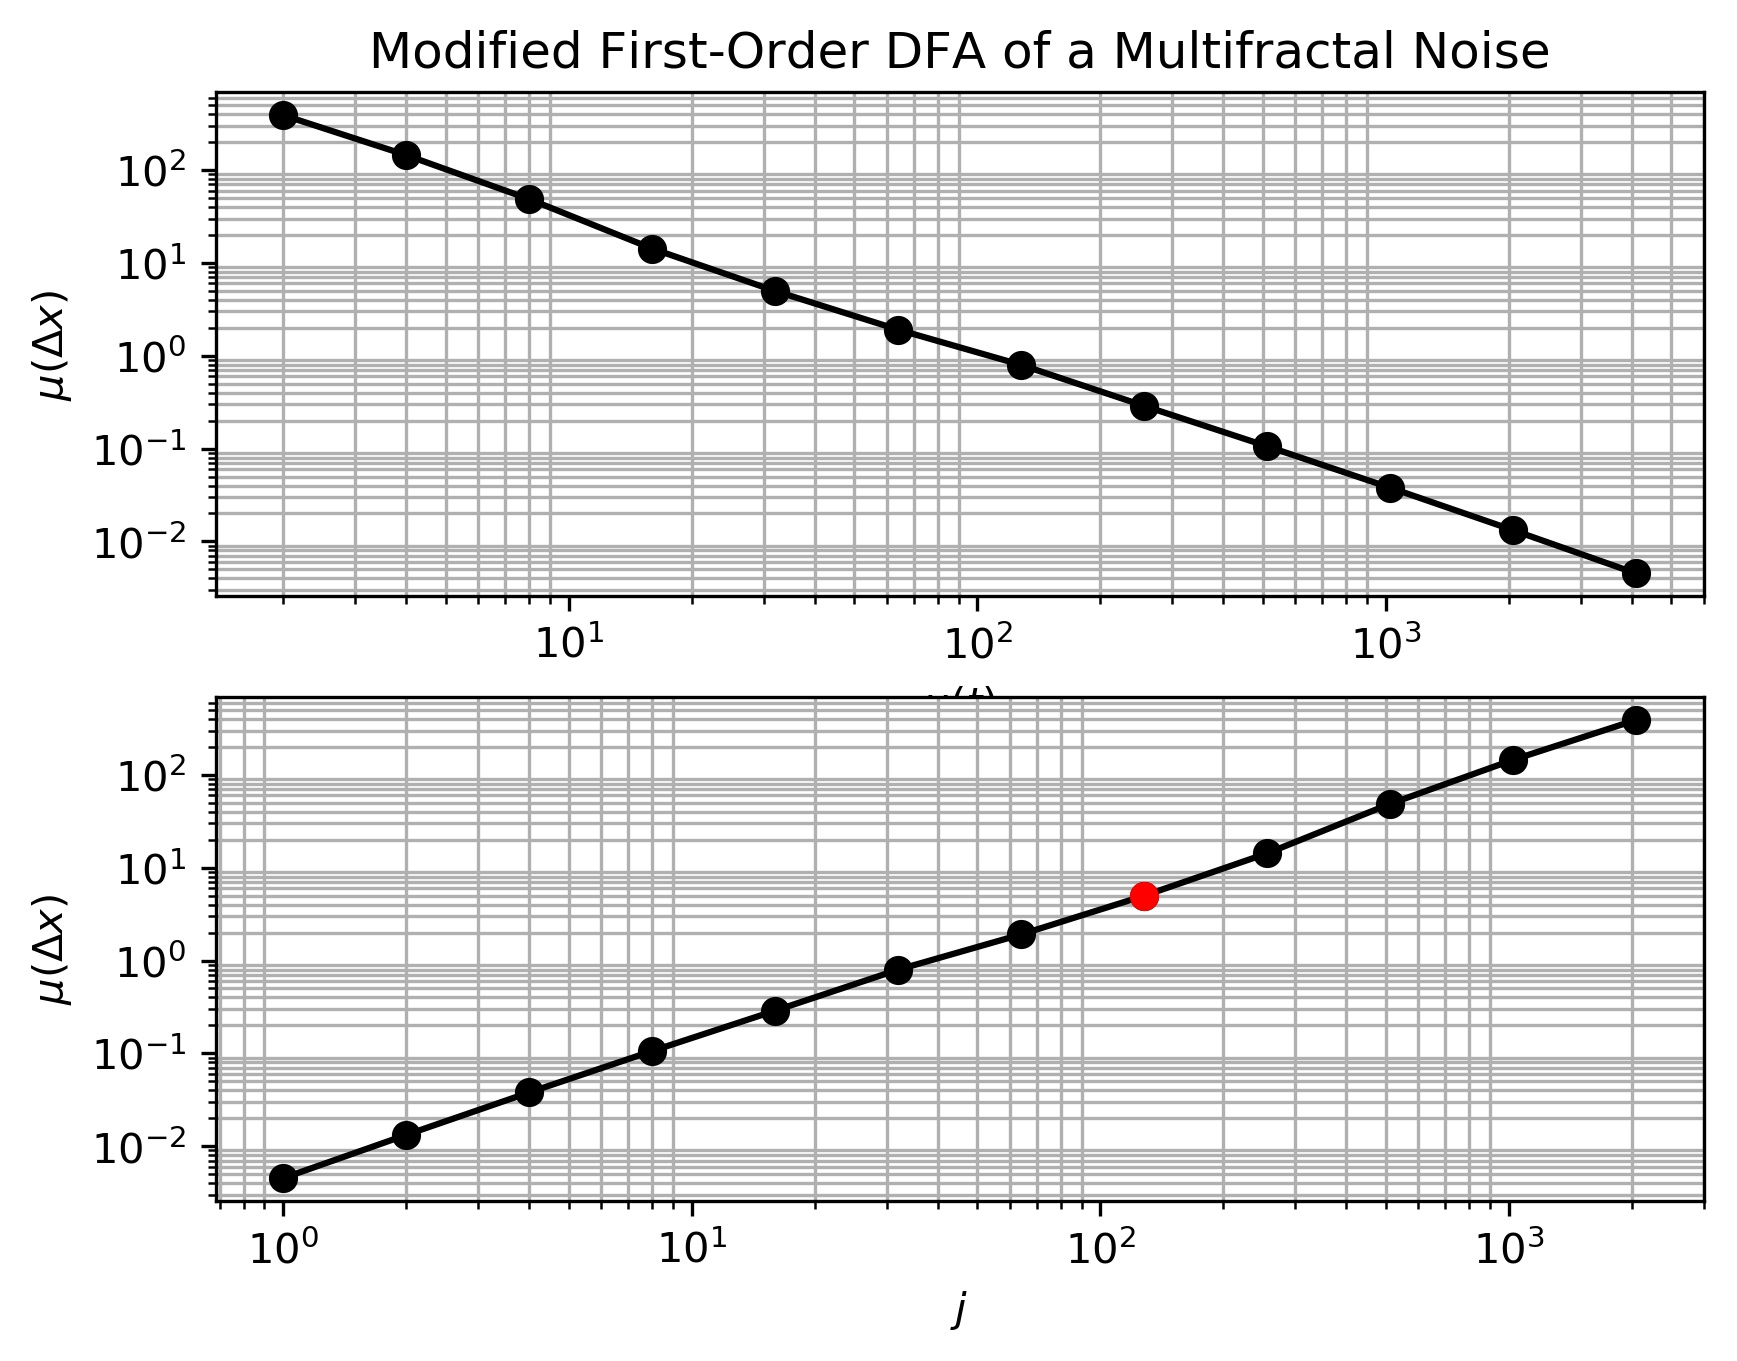
\includegraphics{Figuras/ex7/7_2/Exercicio7_2_grupo_noise_n_8192_mfdfa_1.jpg}}		
	\end{center}
	\vspace{-2mm}	% acrescentar o espaçamento vertical apropriado entre a borda inferior da figura e a legenda ou a fonte quando não há legenda (o valor pode ser negativo para subir)
	\legenda{Figura 7.2.1:. Topo: média da função de flutuação x tempo medido nas diferentes escalas; abaixo: média da função de flutuação x escala. Ambos os plots em log-log. Grupo noise com $n$ = 8192.}	% legenda - para deixar sem legenda usar comando \legenda{} (nunca deve-se comentar o comando \legenda)
	\label{ex6_fig1}
	%\FONTE{}	% fonte consultada (elemento obrigatório, mesmo que seja produção do próprio autor)
\end{figure}

\begin{figure}[ht!]
	%\caption{Série e histogramas.}
	\vspace{0mm}	% acrescentar o espaçamento vertical apropriado entre o título e a borda superior da figura
	\begin{center}
		\resizebox{13cm}{!}{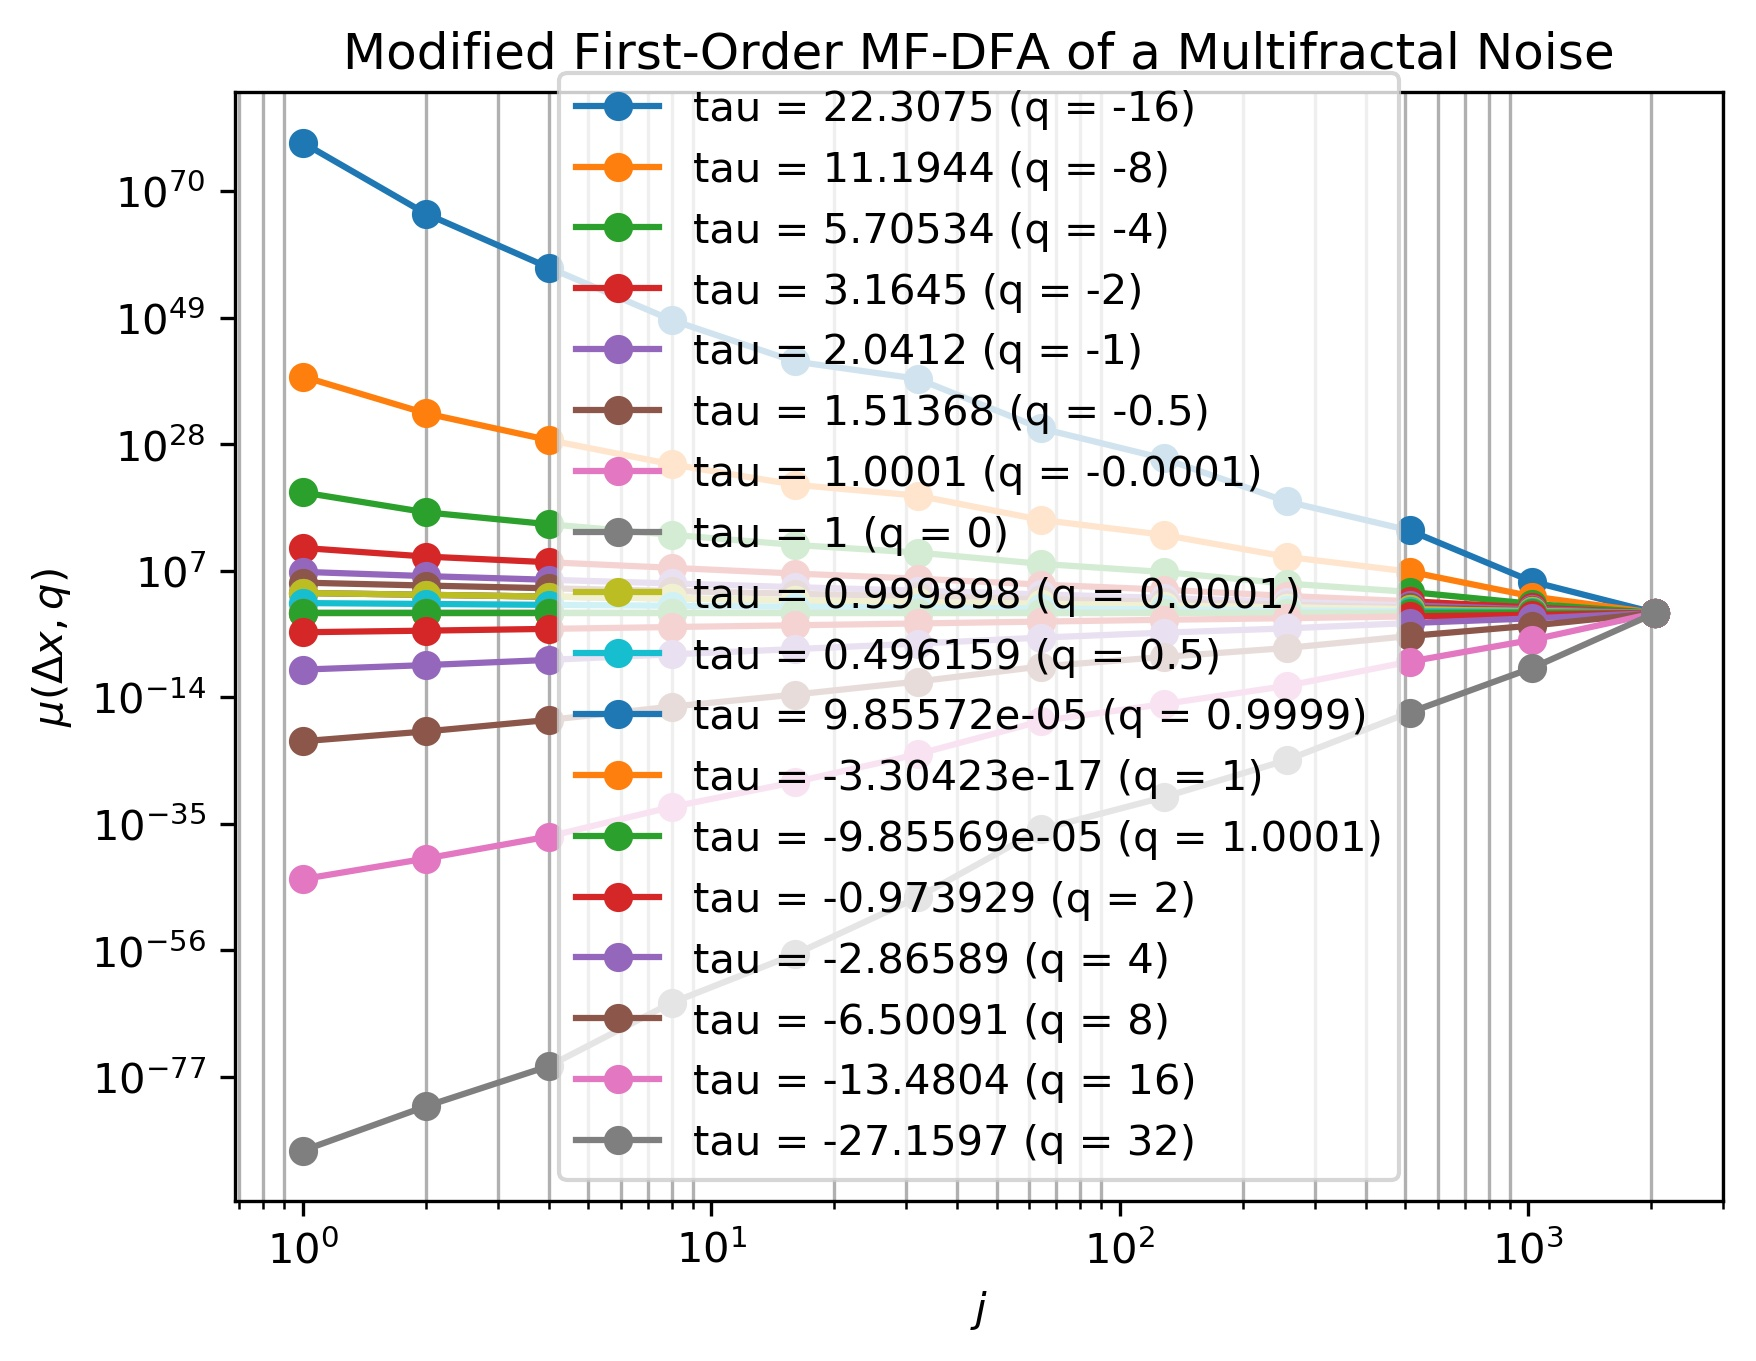
\includegraphics{Figuras/ex7/7_2/Exercicio7_2_grupo_noise_n_8192_mfdfa_2.jpg}}		
	\end{center}
	\vspace{-2mm}	% acrescentar o espaçamento vertical apropriado entre a borda inferior da figura e a legenda ou a fonte quando não há legenda (o valor pode ser negativo para subir)
	\legenda{Figura 7.2.2: Função de flutuação x escala em plot log-log para diferentes valores do expoente $q$. Grupo noise com $n$ = 8192.}	% legenda - para deixar sem legenda usar comando \legenda{} (nunca deve-se comentar o comando \legenda)
	\label{ex6_fig1}
	%\FONTE{}	% fonte consultada (elemento obrigatório, mesmo que seja produção do próprio autor)
\end{figure}

\begin{figure}[ht!]
	%\caption{Série e histogramas.}
	\vspace{0mm}	% acrescentar o espaçamento vertical apropriado entre o título e a borda superior da figura
	\begin{center}
		\resizebox{13cm}{!}{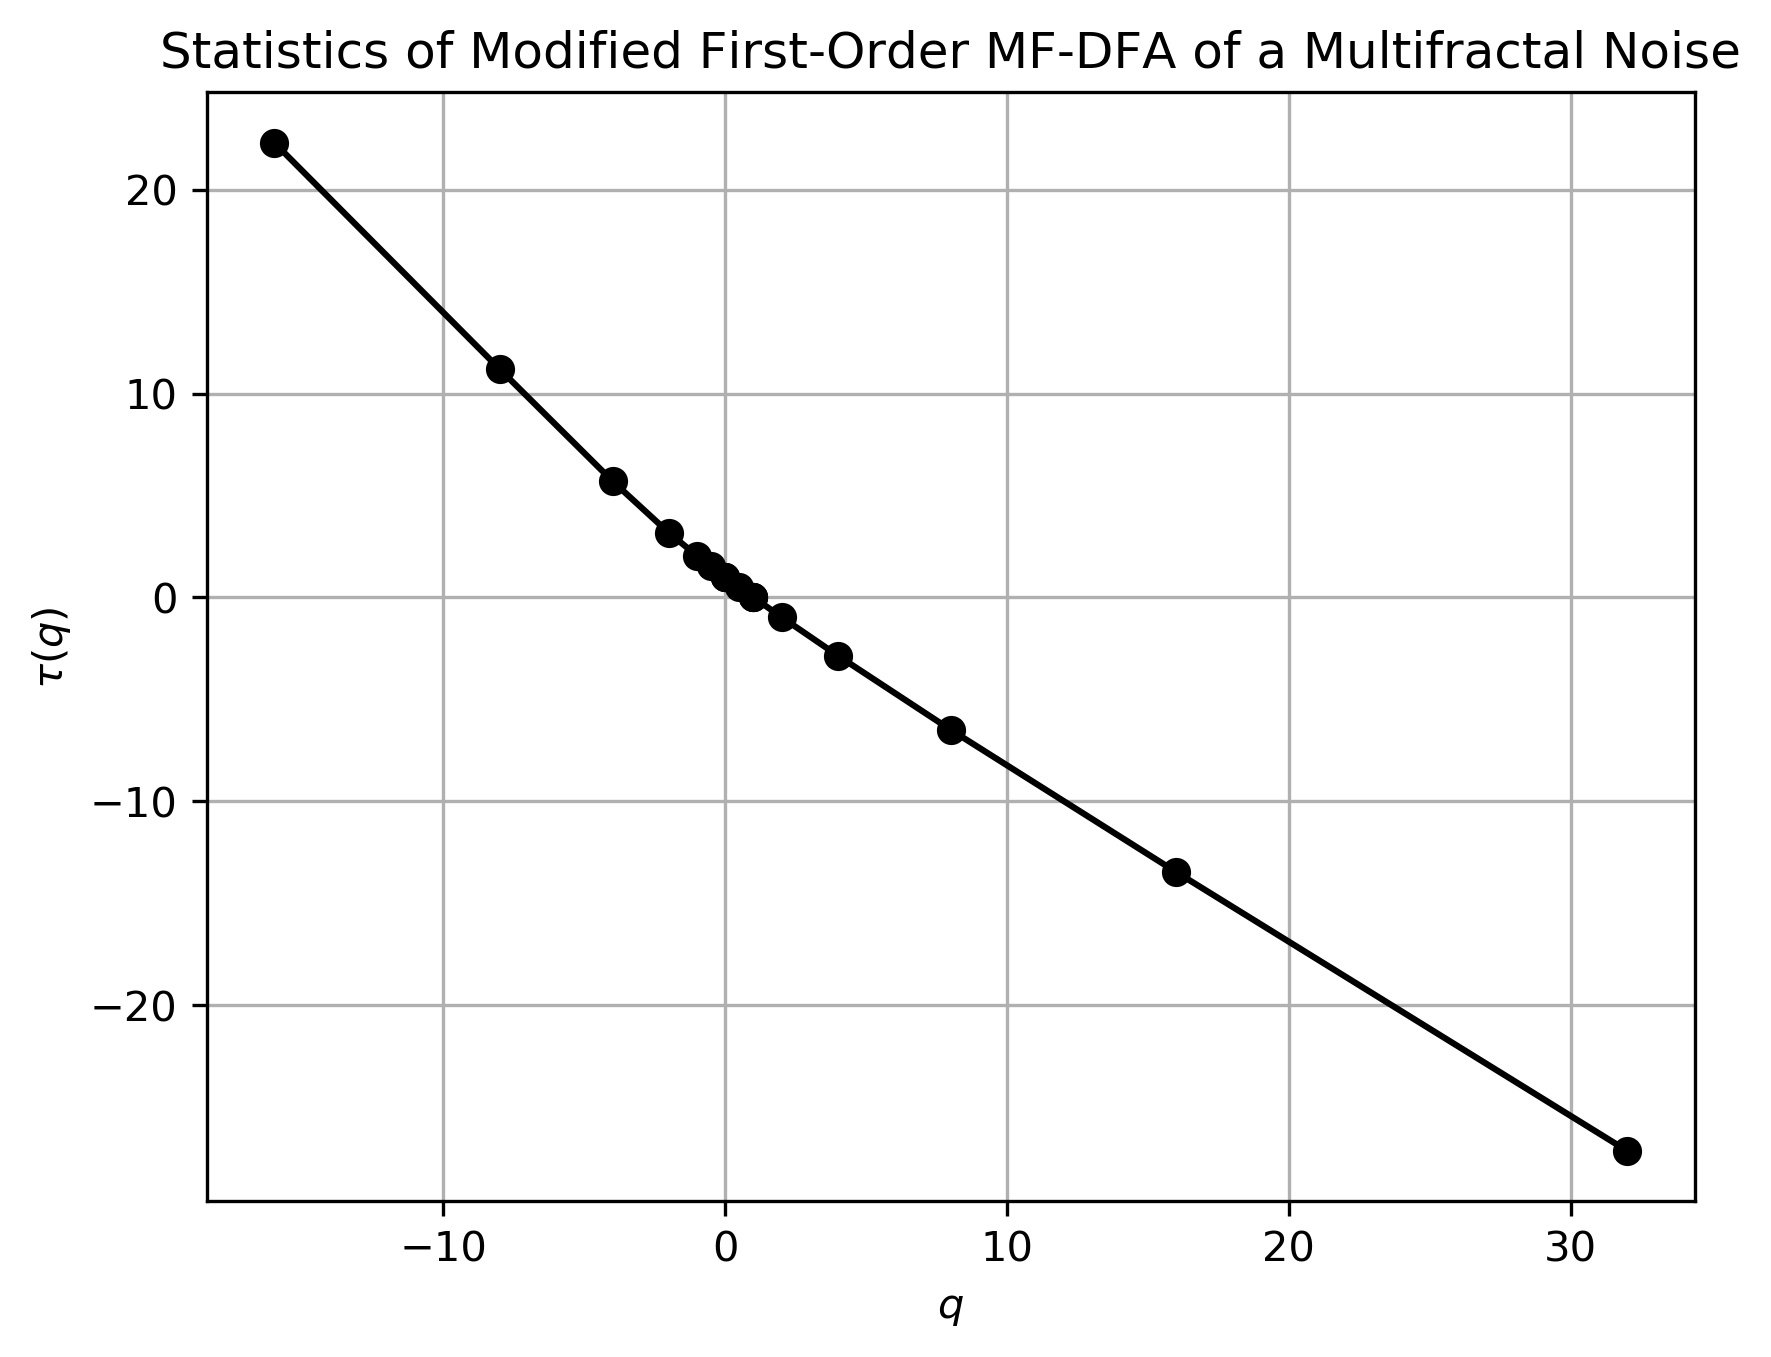
\includegraphics{Figuras/ex7/7_2/Exercicio7_2_grupo_noise_n_8192_mfdfa_3.jpg}}		
	\end{center}
	\vspace{-2mm}	% acrescentar o espaçamento vertical apropriado entre a borda inferior da figura e a legenda ou a fonte quando não há legenda (o valor pode ser negativo para subir)
	\legenda{Figura 7.2.3: Dependência de $\tau(q)$ com $q$ do grupo noise para $n$ = 8192.}	% legenda - para deixar sem legenda usar comando \legenda{} (nunca deve-se comentar o comando \legenda)
	\label{ex6_fig1}
	%\FONTE{}	% fonte consultada (elemento obrigatório, mesmo que seja produção do próprio autor)
\end{figure}
\clearpage
\begin{figure}[ht!]
	%\caption{Série e histogramas.}
	\vspace{0mm}	% acrescentar o espaçamento vertical apropriado entre o título e a borda superior da figura
	\begin{center}
		\resizebox{13cm}{!}{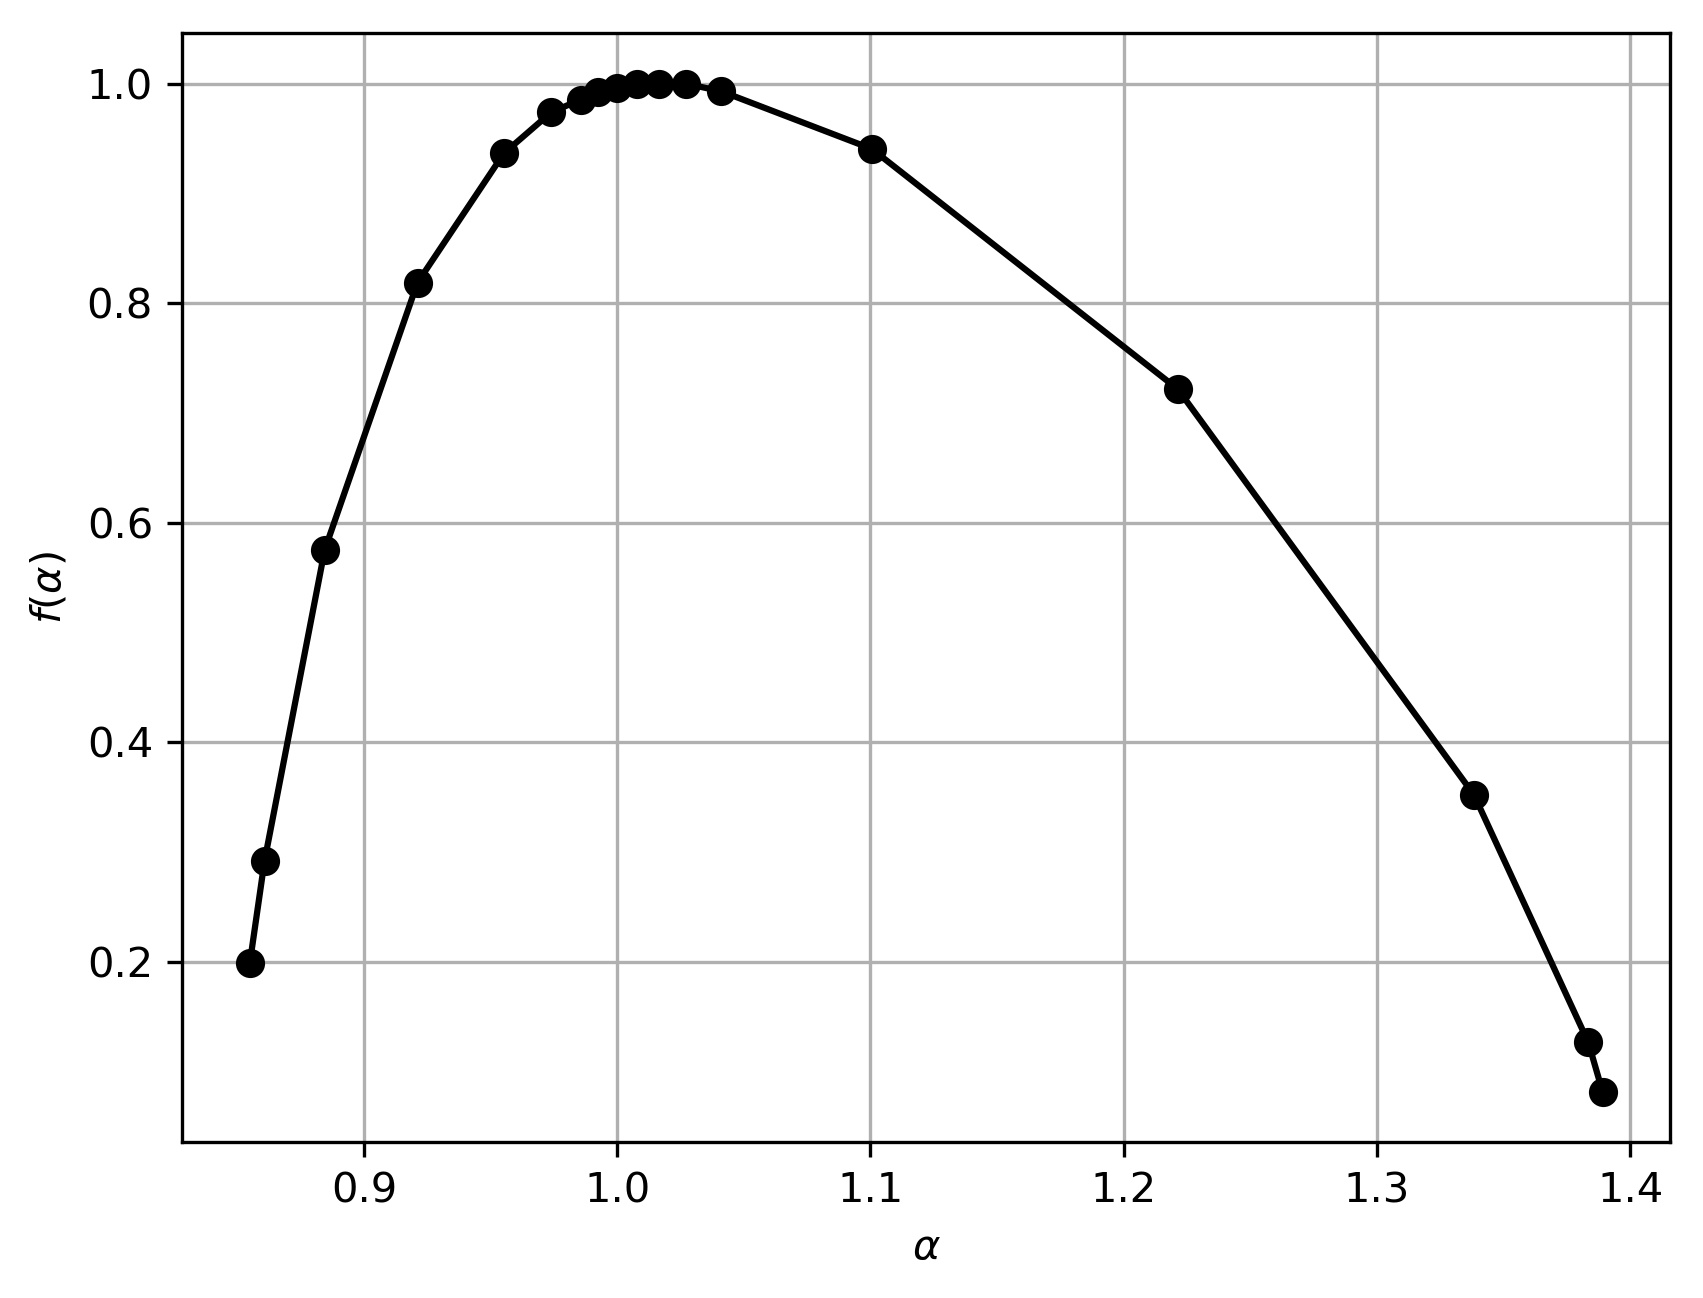
\includegraphics{Figuras/ex7/7_2/Exercicio7_2_grupo_noise_n_8192_mfdfa_4.jpg}}		
	\end{center}
	\vspace{-2mm}	% acrescentar o espaçamento vertical apropriado entre a borda inferior da figura e a legenda ou a fonte quando não há legenda (o valor pode ser negativo para subir)
	\legenda{Figura 7.2.4: Espectro de singularidade $f(\alpha)$ vs $\alpha$ do grupo noise com $n$ = 8192.}	% legenda - para deixar sem legenda usar comando \legenda{} (nunca deve-se comentar o comando \legenda)
	\label{ex6_fig1}
	%\FONTE{}	% fonte consultada (elemento obrigatório, mesmo que seja produção do próprio autor)
\end{figure}


%%%%%%%%%%%%%%%%%%%%%%%%%%%%%%%%%%% Analise extra %%%%%%%%%%%%%%
%\clearpage
\subsubsection*{Monofractalidade vs Multifractalidade}

Uma análise interessante é a comparação do espectro de singularidade entre dois grupos particulares da tabela \textit{Dataset\_signal}: chaosnoise e pmnoise. O espectro de singularidade para o mapeamento Logístico e para uma série exógena (Figura 7.2.5) são apresentados a seguir.

O valor de $\Delta \alpha$ = $\alpha_{max} - \alpha_{min}$ reflete a multifractalidade da série. Quanto maior $\Delta \alpha$, maior a característica multifractal e complexidade da série, e a distribuição apresenta flutuações mais severas. Mapas caóticos como o mapeamento Logístico possuem uma faixa dinâmica estreita e apresentam monofractalidade, de modo que seu espectro de singularidade indica um valor de $\Delta \alpha$ relativamente pequeno: a curva em vermelho da Figura 7.2.5 não se extende nas duas extremidades (ela é monofractal-like). Por outro lado, a série exógena do pmodel apresenta multifractalidade, de forma que seu $\Delta \alpha$ é maior conforme evidenciado pelo espectro de singularidade.

\begin{figure}[ht!]
	%\caption{Série e histogramas.}
	\vspace{0mm}	% acrescentar o espaçamento vertical apropriado entre o título e a borda superior da figura
	\begin{center}
		\resizebox{16cm}{!}{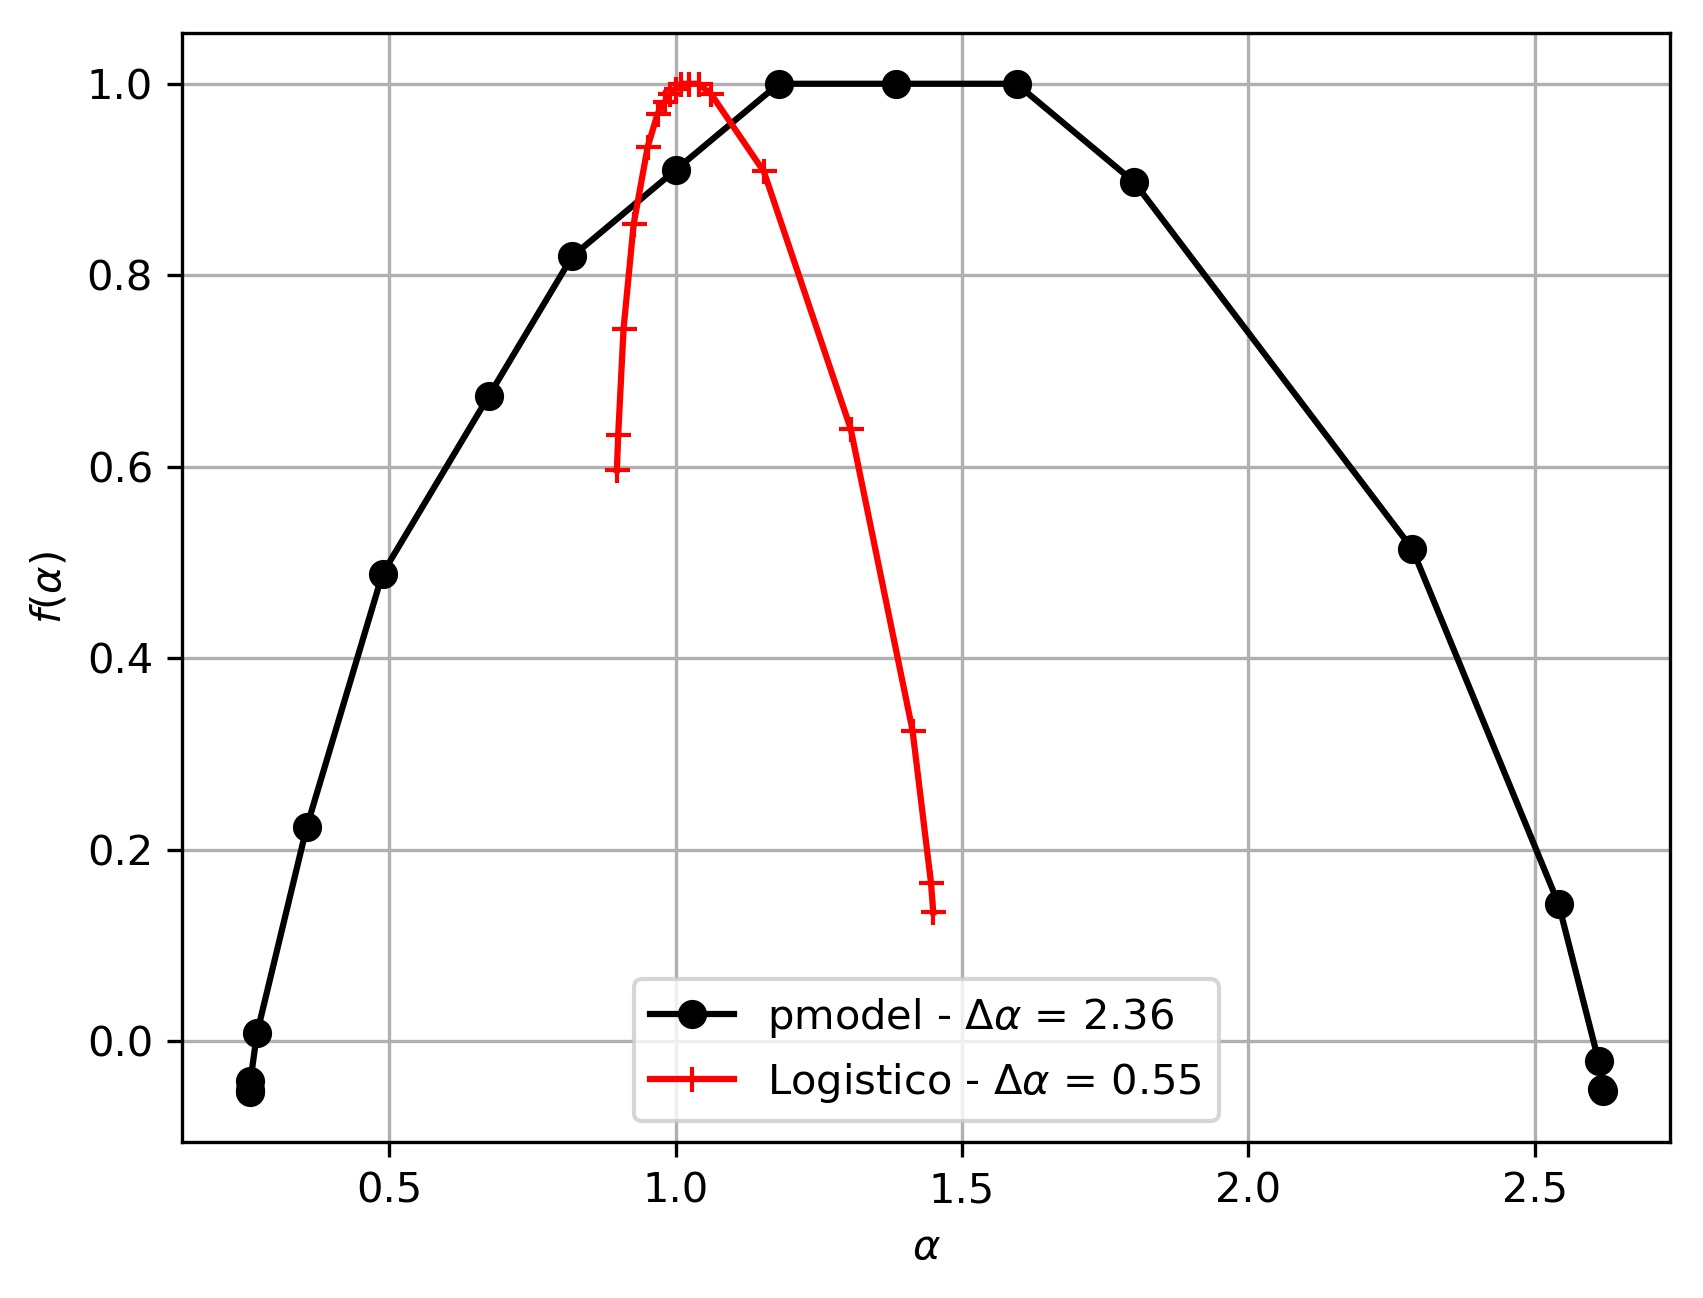
\includegraphics{Figuras/ex7/7_2/comp_mfdfa_4.jpg}}		
	\end{center}
	\vspace{-2mm}	% acrescentar o espaçamento vertical apropriado entre a borda inferior da figura e a legenda ou a fonte quando não há legenda (o valor pode ser negativo para subir)
	\legenda{Figura 7.2.5: Comparação entre o espectro de singularidade $f(\alpha)$ vs $\alpha$ do grupo pmnoise e do grupo chaosnoise. Série exógena do pmodel com $p$ = 0.18 e $\beta$ = 0.7 vs mapeamento Logístico com $\rho$ = 3.81.}	% legenda - para deixar sem legenda usar comando \legenda{} (nunca deve-se comentar o comando \legenda)
	\label{ex6_fig1}
	%\FONTE{}	% fonte consultada (elemento obrigatório, mesmo que seja produção do próprio autor)
\end{figure}

%\begin{figure}[ht!]
	%\caption{Série e histogramas.}
%	\vspace{-3mm}	% acrescentar o espaçamento vertical apropriado entre o título e a borda superior da figura
%	\begin{center}
%		\resizebox{12cm}{!}{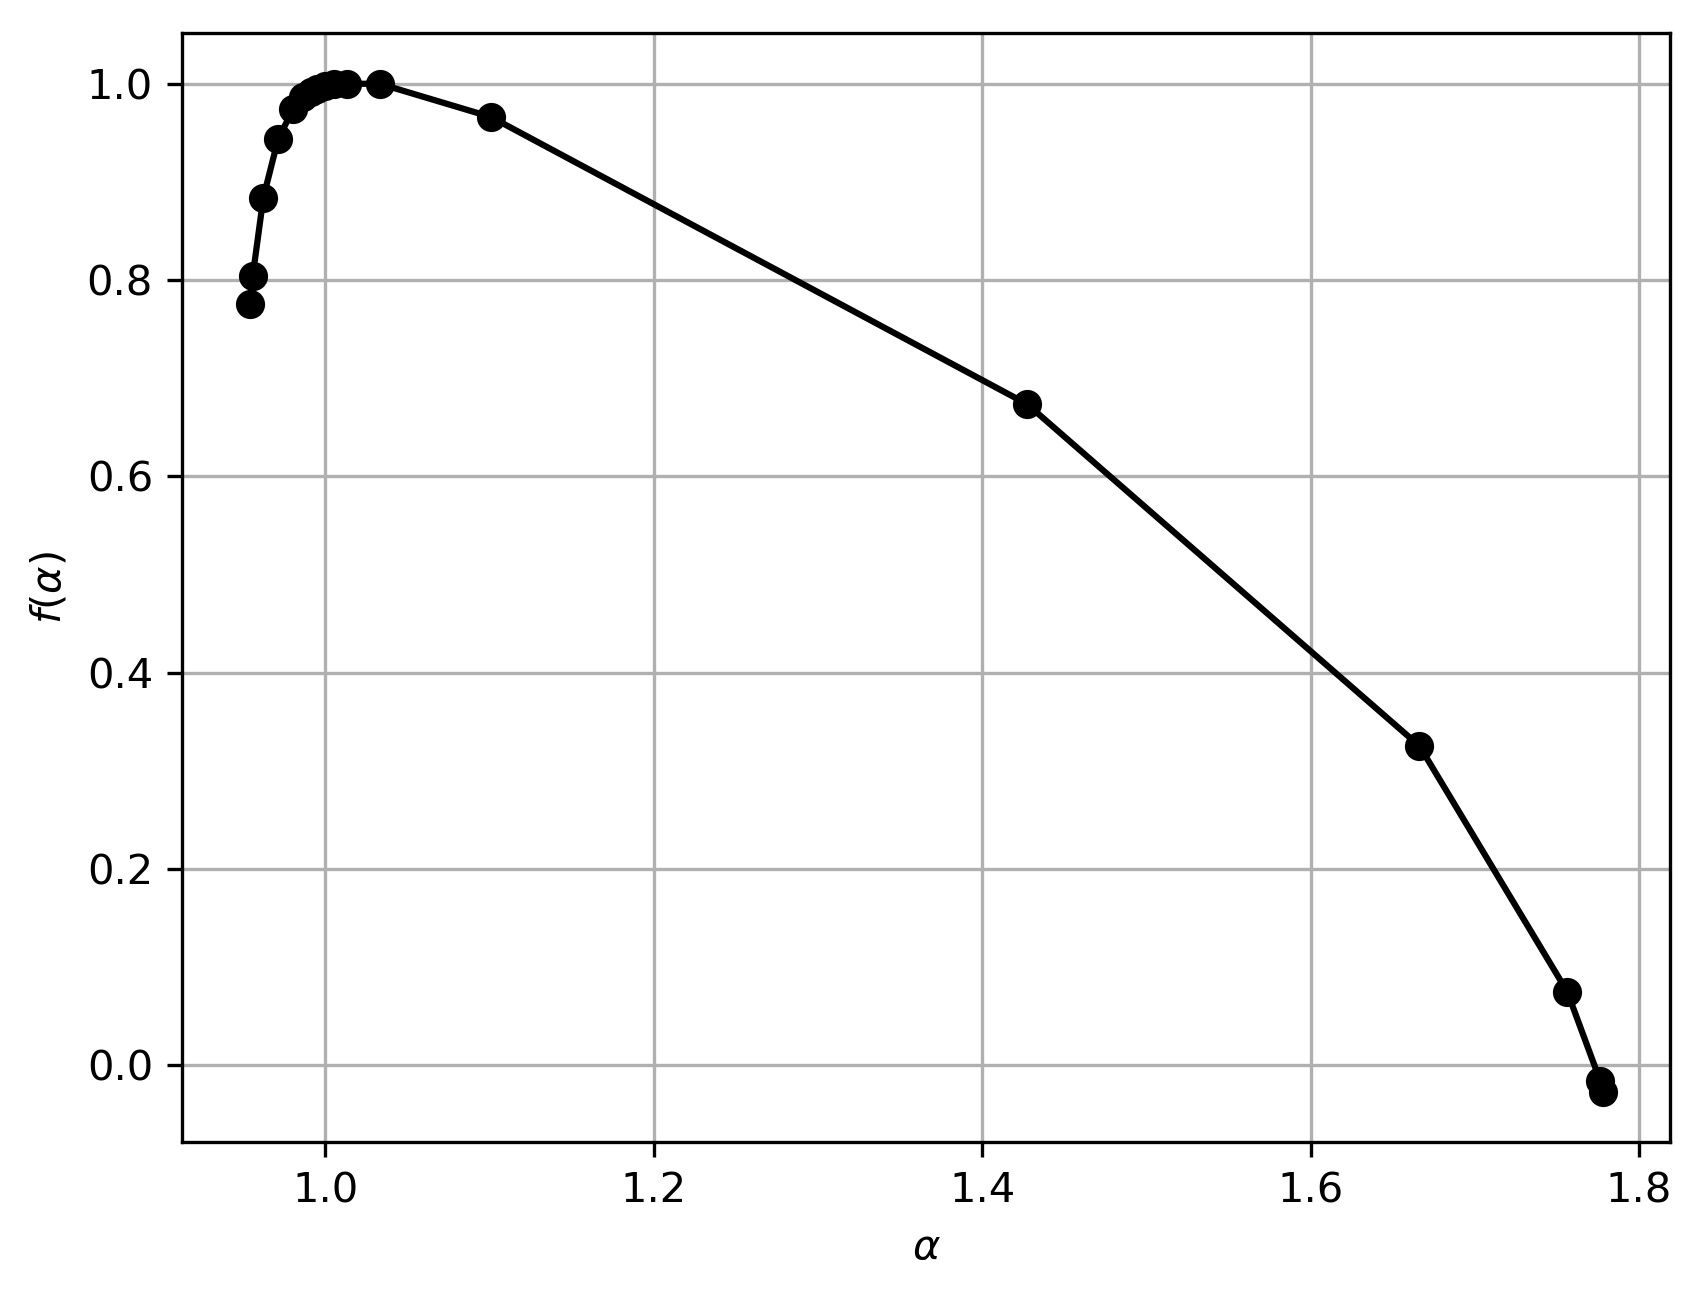
\includegraphics{Figuras/ex7/7_2/Exercicio7_2_Logistico_rho_3.81_mfdfa_4.jpg}}		
%	\end{center}
%	\vspace{-3mm}	% acrescentar o espaçamento vertical apropriado entre a borda inferior da figura e a legenda ou a fonte quando não há legenda (o valor pode ser negativo para subir)
%	\legenda{Figura 7.2.5: Espectro de singularidade $f(\alpha)$ vs $\alpha$ do grupo chaosnoise: mapeamento Logístico com $\rho$ = 3.81.}	% legenda - para deixar sem legenda usar comando \legenda{} (nunca deve-se comentar o comando \legenda)
%	\label{ex6_fig1}
	%\FONTE{}	% fonte consultada (elemento obrigatório, mesmo que seja produção do próprio autor)
%\end{figure}

%\begin{figure}[ht!]
	%\caption{Série e histogramas.}
%	\vspace{-3mm}	% acrescentar o espaçamento vertical apropriado entre o título e a borda superior da figura
%	\begin{center}
%		\resizebox{12cm}{!}{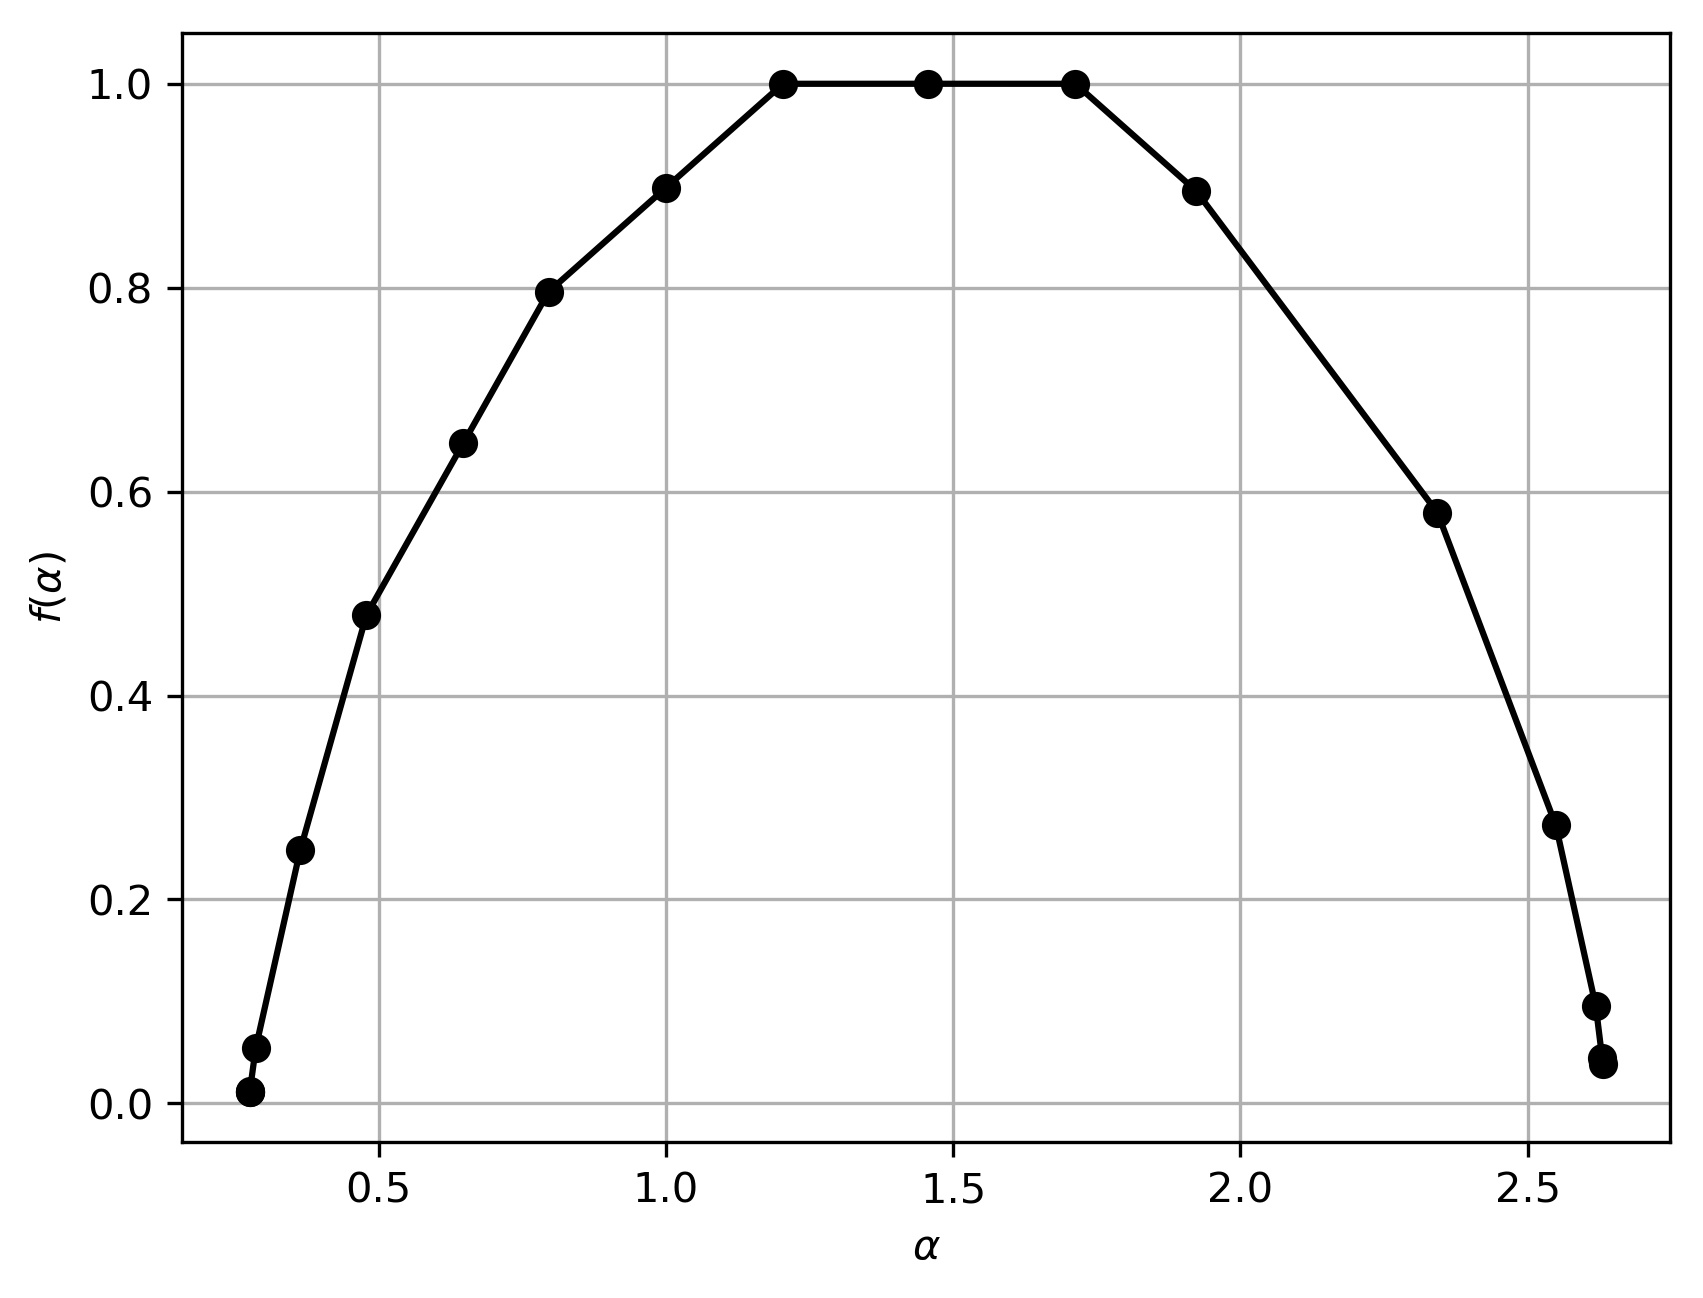
\includegraphics{Figuras/ex7/7_2/Exercicio7_2_grupo_pmnoise_p_0.18_mfdfa_4.jpg}}		
%	\end{center}
%	\vspace{-3mm}	% acrescentar o espaçamento vertical apropriado entre a borda inferior da figura e a legenda ou a fonte quando não há legenda (o valor pode ser negativo para subir)
%	\legenda{Figura 7.2.6: Espectro de singularidade $f(\alpha)$ vs $\alpha$ do grupo pmnoise: série exógena com $p$ = 0.18 e $\beta$ = 0.7.}	% legenda - para deixar sem legenda usar comando \legenda{} (nunca deve-se comentar o comando \legenda)
%	\label{ex6_fig1}
	%\FONTE{}	% fonte consultada (elemento obrigatório, mesmo que seja produção do próprio autor)
%\end{figure}


%%%%%%%%%%%%%%%%%%%%%%%%%%%%%%%%%%%  7.3 %%%%%%%%%%%%%%%%%%%%%%%%%%%%
\clearpage
\subsection*{7.3}
\addcontentsline{toc}{section}{\protect\numberline{} 7.3}%

Os resultados deste exercício estão presentes na pasta \textbf{7.3}. Abaixo o plot do melhor número de clusters determinado pelo méotodo do cotovelo. O algoritmo utilizado foi o kmeans\_2D\_group\_flags.py, que agrupou cada país em seu respectivo cluster em arquivos .csv (identificados pelo centróide do grupo).

\begin{figure}[ht!]
	%\caption{Série e histogramas.}
	\vspace{0mm}	% acrescentar o espaçamento vertical apropriado entre o título e a borda superior da figura
	\begin{center}
		\resizebox{15cm}{!}{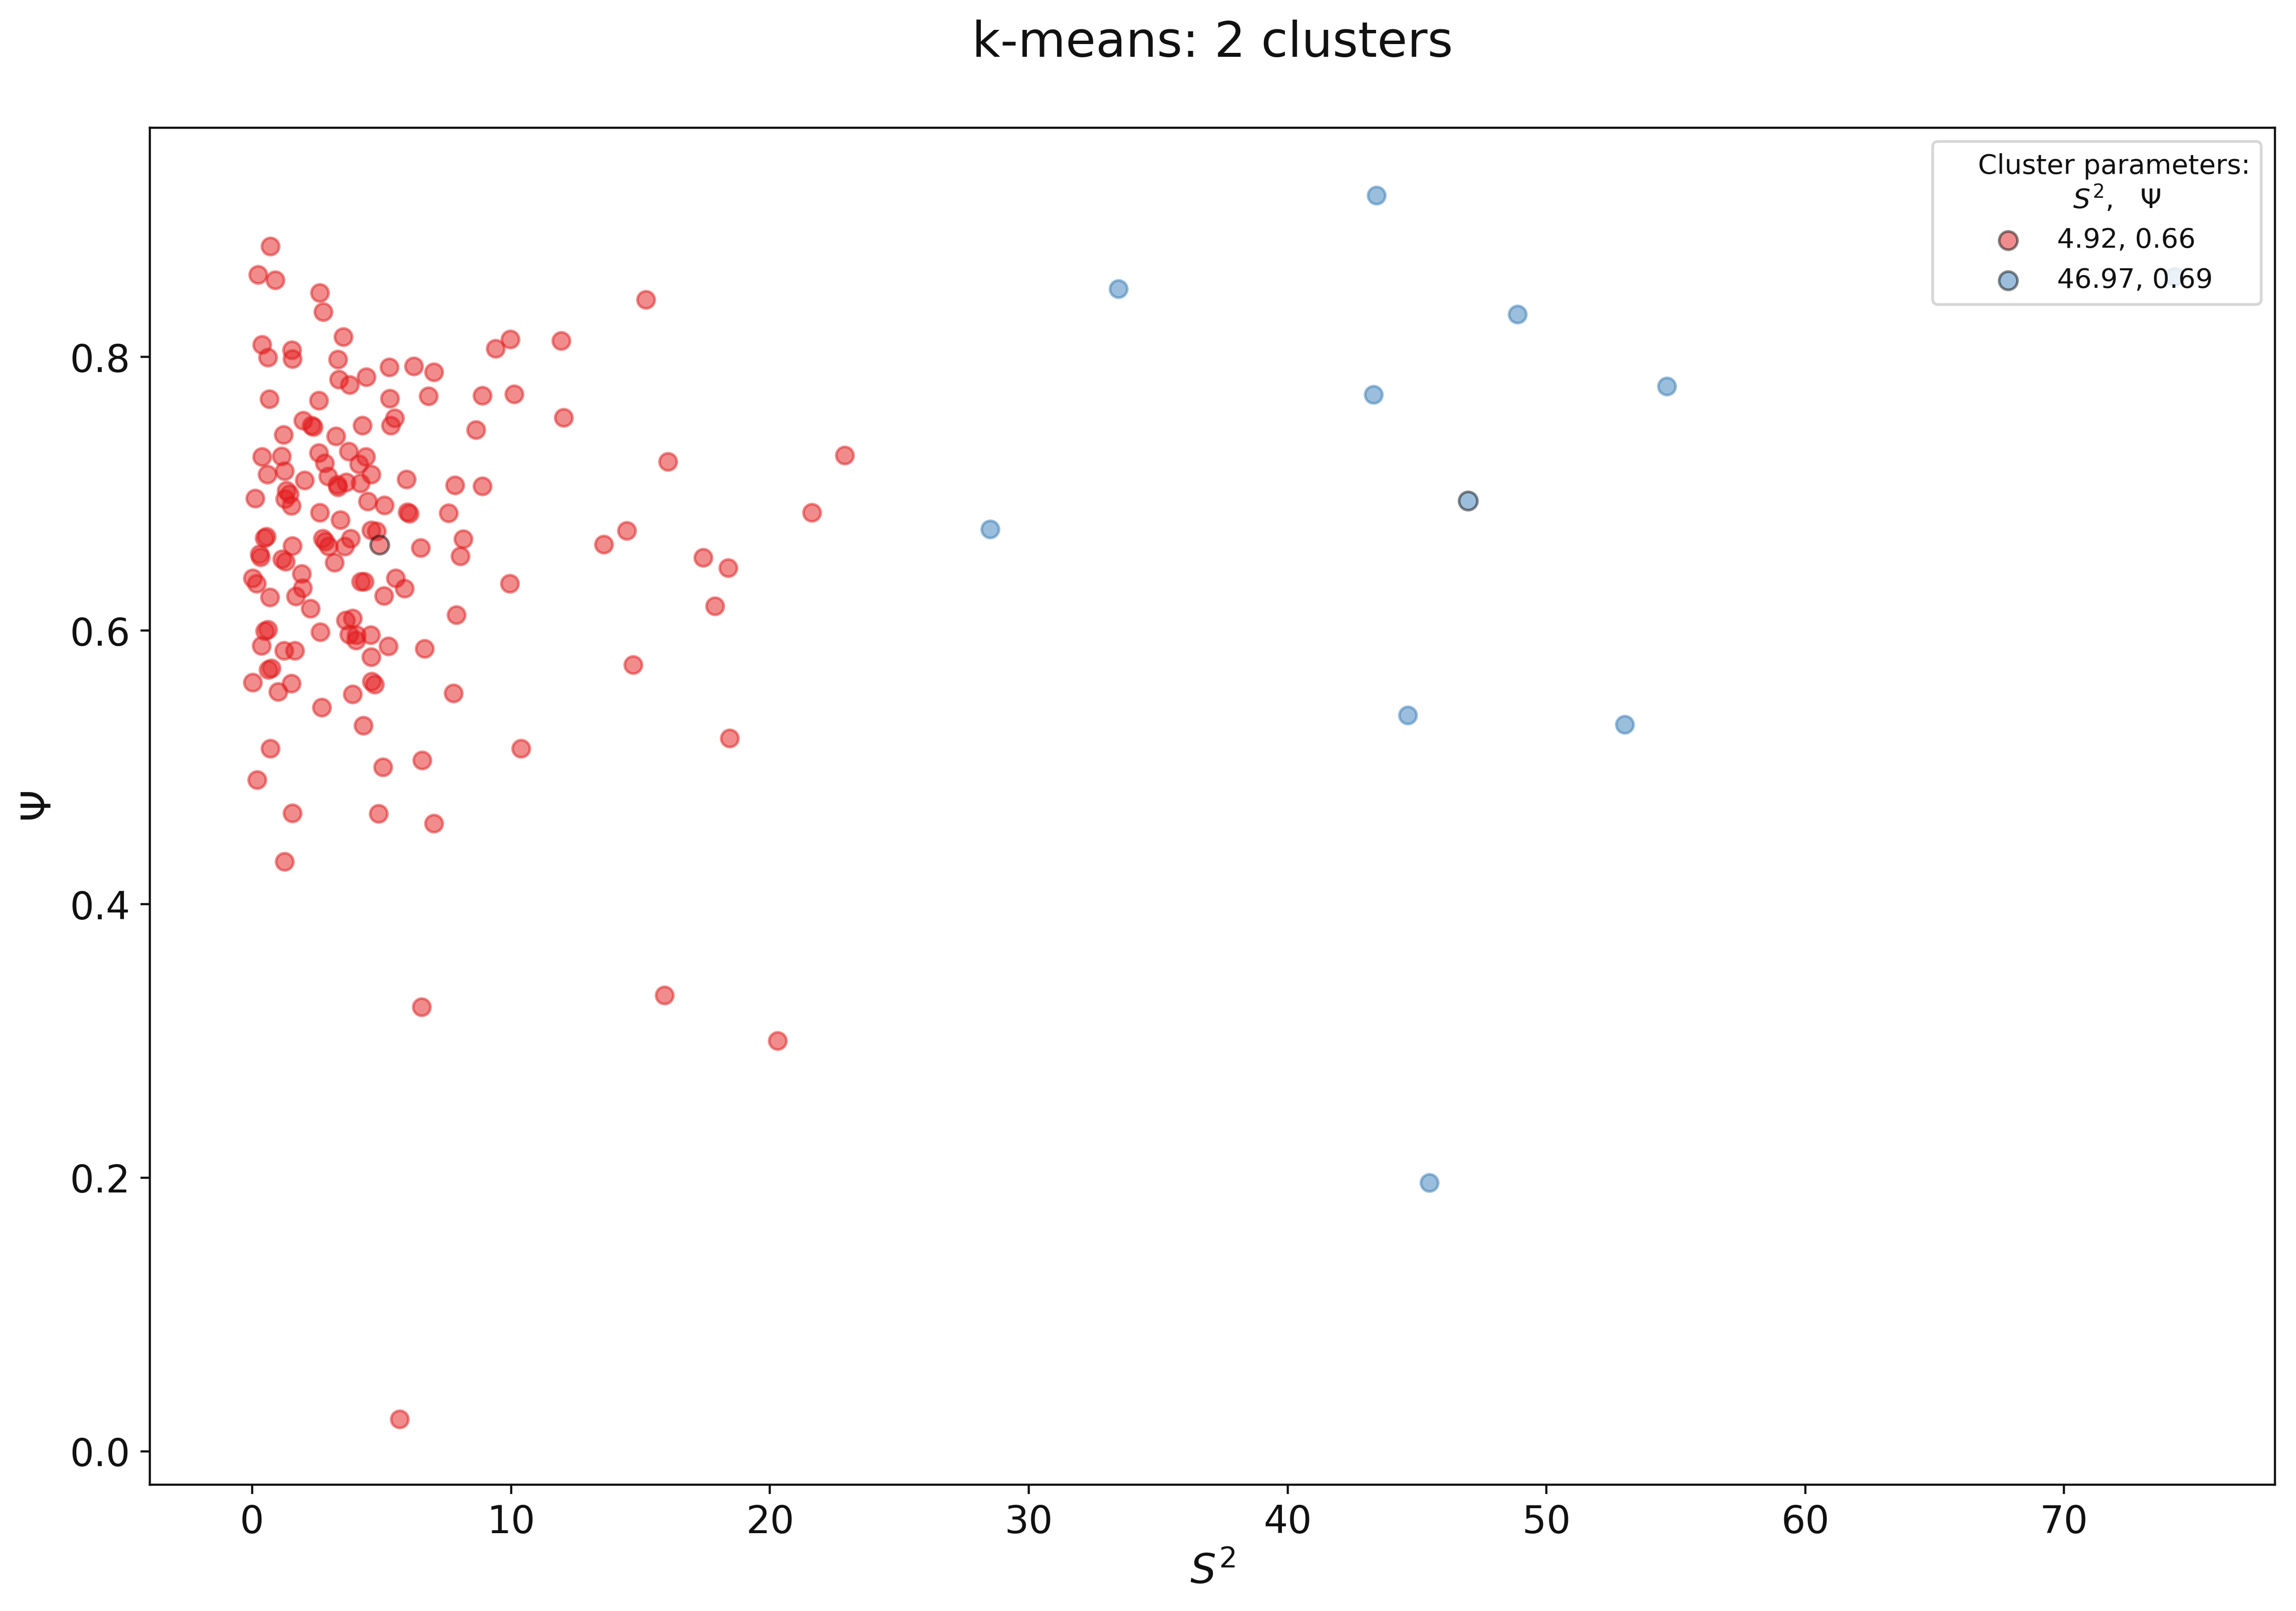
\includegraphics{Figuras/ex7/7_3/Exercicio7_3_cluster_2.jpg}}		
	\end{center}
	\vspace{-2mm}	% acrescentar o espaçamento vertical apropriado entre a borda inferior da figura e a legenda ou a fonte quando não há legenda (o valor pode ser negativo para subir)
	\legenda{Figura 7.3.1: Resultado do agrupamento do número de casos diários de Covid19 para todos os países no espaço S$^{2}$ x $\Psi$. O valor $n\_c$ = 2 obteve a melhor performance.}	% legenda - para deixar sem legenda usar comando \legenda{} (nunca deve-se comentar o comando \legenda)
	\label{ex6_fig1}
	%\FONTE{}	% fonte consultada (elemento obrigatório, mesmo que seja produção do próprio autor)
\end{figure}

Neste exercício, os grupos de países se encontram nos seguintes arquivos: \textit{Exercicio7\_3\_cluster\_0\_x\_3.58\_y\_0.62\_flags.csv} (cluster vemelho) e \textit{Exercicio7\_3\_cluster\_1\_x\_36.38\_y\_0.62\_flags.csv} (cluster azul). %% 3o capítulo

\clearpage
%%%%%%%%%%%%%%%%%%%%%%%%%%%%%%%%%%%%%%%%%%%%%%%%%%%%%%%%%%%%%%%%%%%%%%%%%%%%%%%

\section*{\large Exercício 8 - Global Wavelet Spectrum}
\addcontentsline{toc}{chapter}{\protect\numberline{}\large Exercício 8}%

Os resultados deste exercício se encontram na pasta \textbf{Exercise8}. Abaixo está a análise para a série de novos casos da Covid19 para o Brasil, de 30 de março a 5 de junho. Foi utilizado o pacode do Python waipy.

Os plots das ondeletas mãe Morlet e DoG (Derivative of Gaussian) indicam que a melhor escolha é a DoG, pois ela foi capaz de captar os períodos do sinal dentro do cone de influência, com um pico bem pronunciado no wavelet spectrum (Figura 8.2.1). Por outro lado, a ondeleta Morlet não foi capaz de apresentar o pico dentro do cone de influência (Figura 8.1.1).

\subsection*{8.1}
\addcontentsline{toc}{section}{\protect\numberline{} 8.1}%

Resultado da aplicação do pacote waipy com a wavelet mãe Morlet, aplicada sobre a série da Covid19 (novos casos diários) para o Brasil. O período do sinal não é bem captado pela ondeleta: o pico do espectro wavelet - em azul à direita - está fora do cone de influência. 

\begin{figure}[ht!]
	%\caption{Série e histogramas.}
	\vspace{0mm}	% acrescentar o espaçamento vertical apropriado entre o título e a borda superior da figura
	\begin{center}
		\resizebox{16cm}{!}{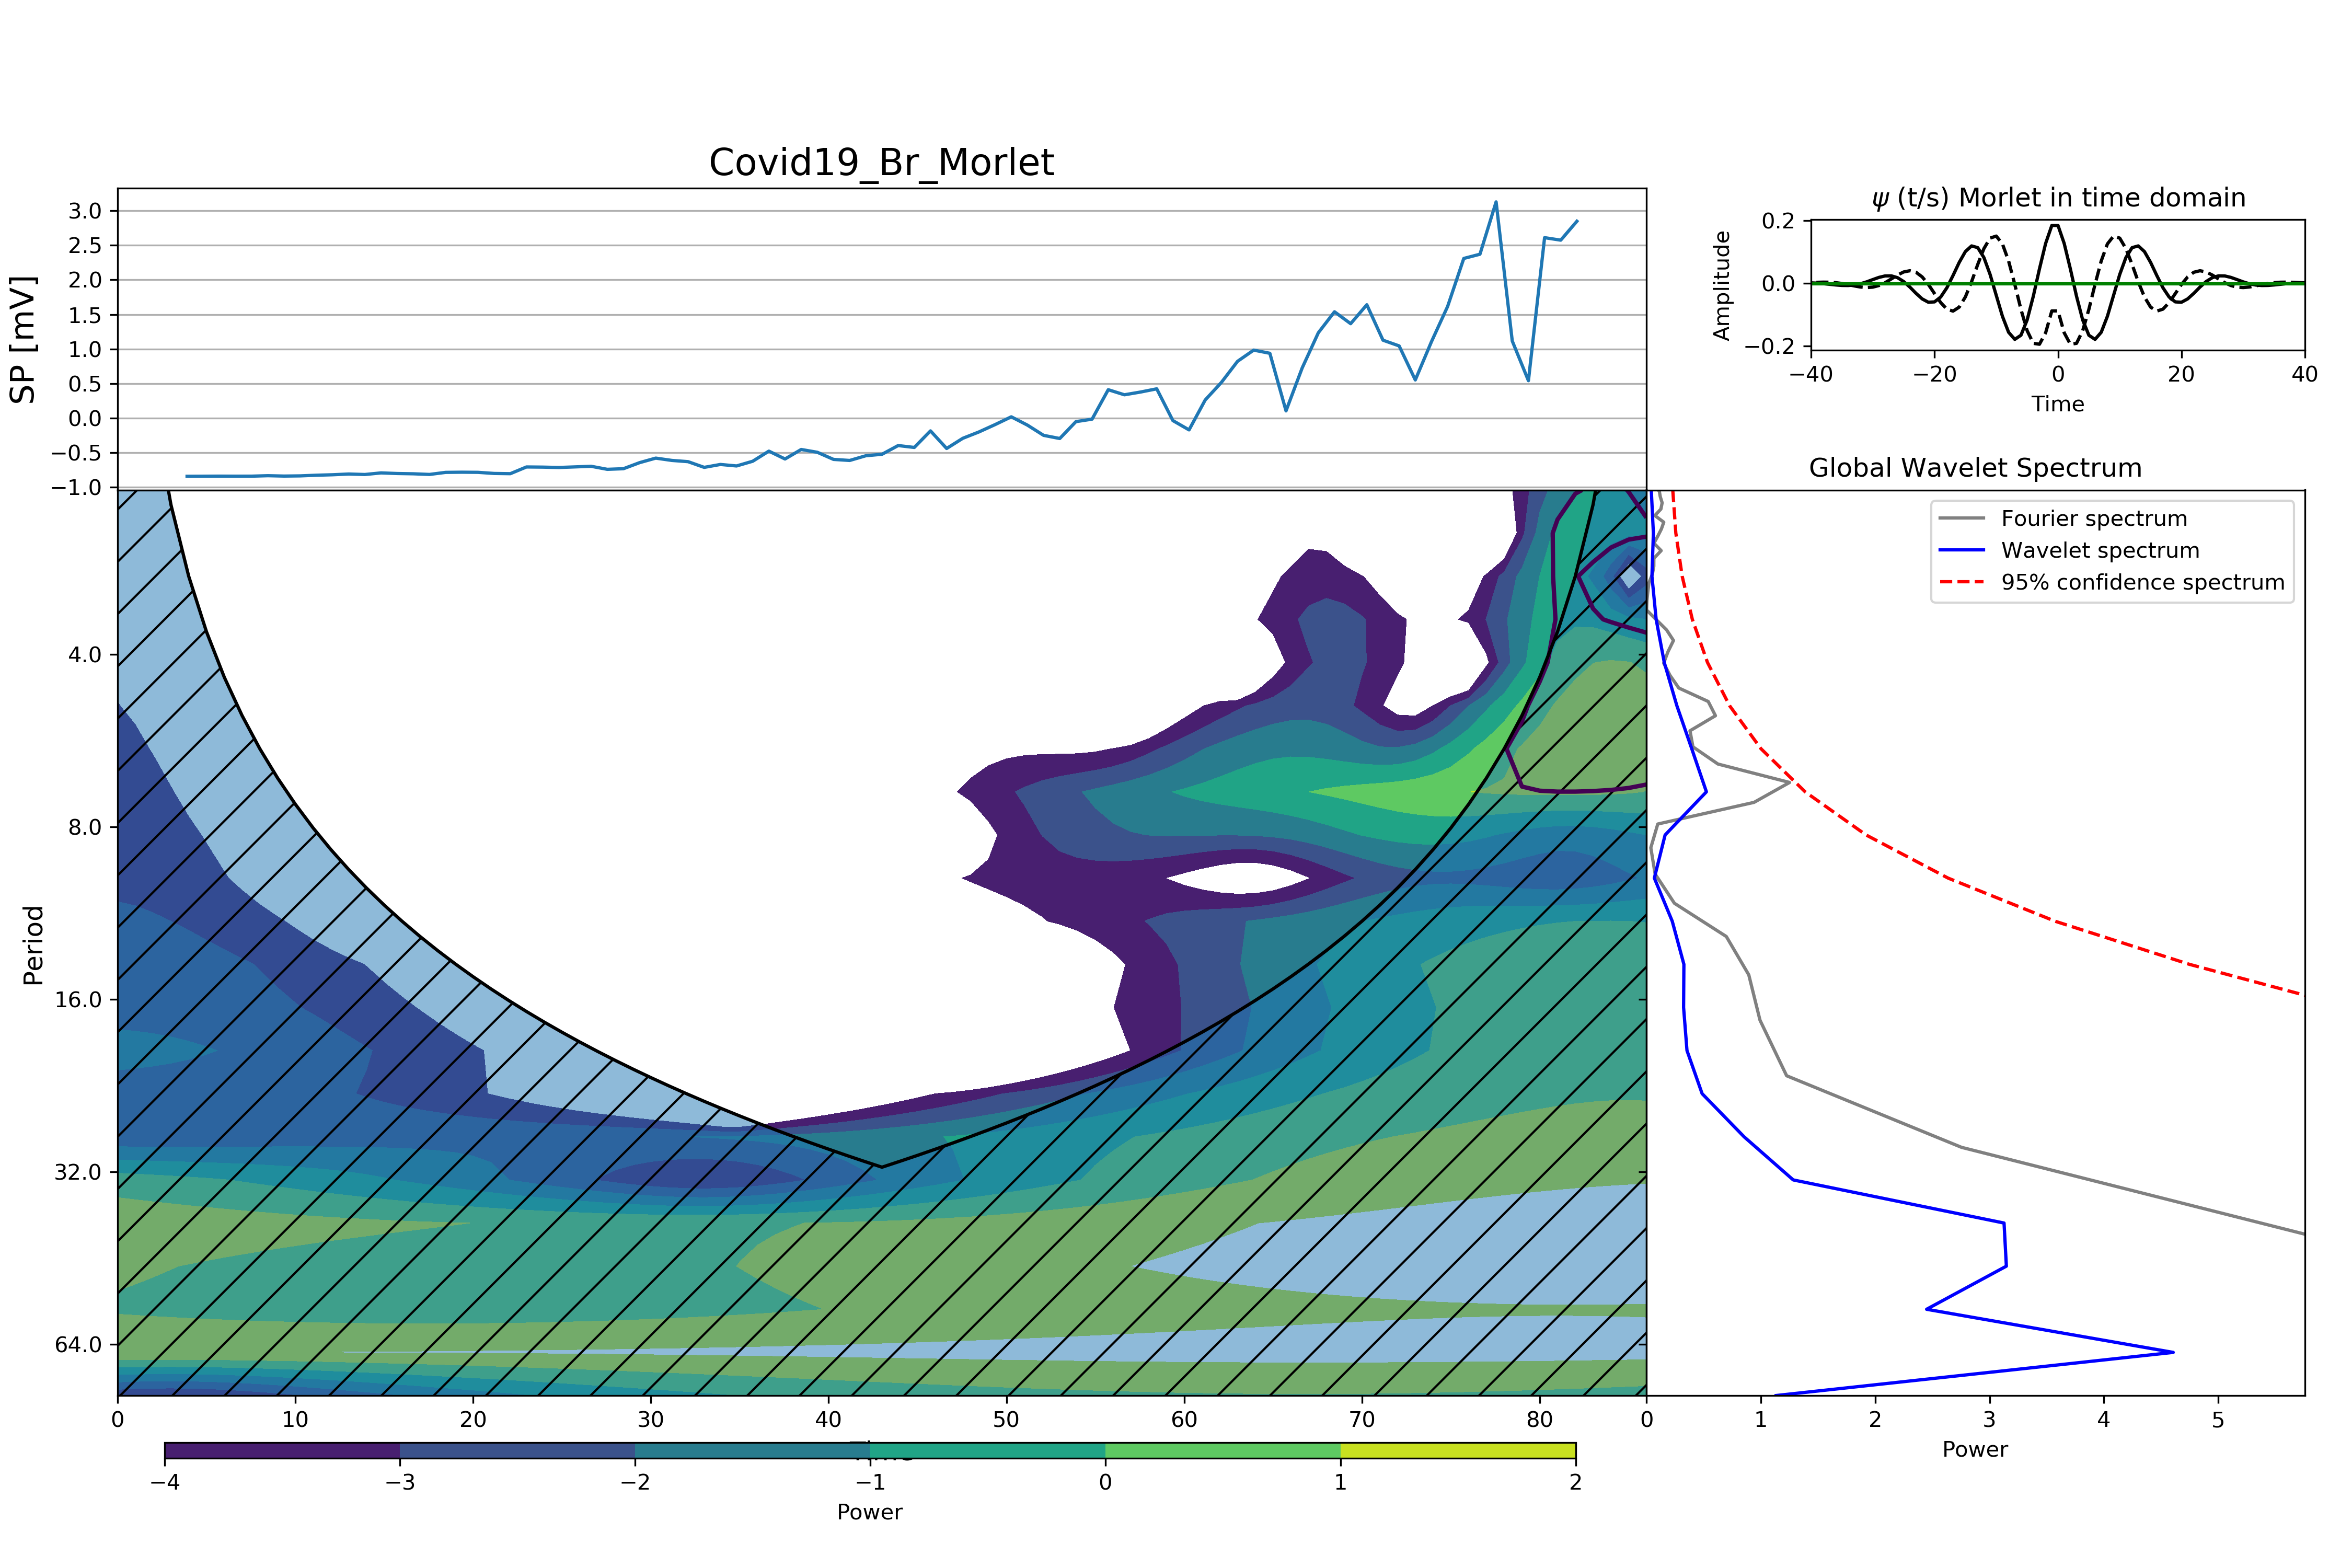
\includegraphics{Figuras/ex8/Covid19_Br_Morlet.png}}		
	\end{center}
	\vspace{-2mm}	% acrescentar o espaçamento vertical apropriado entre a borda inferior da figura e a legenda ou a fonte quando não há legenda (o valor pode ser negativo para subir)
	\legenda{Figura 8.1.1: Global Wavelet Spectrum da série de dados da Covid19 do Brasil com a ondeleta mãe Morlet.}	% legenda - para deixar sem legenda usar comando \legenda{} (nunca deve-se comentar o comando \legenda)
	\label{ex8_fig1}
	%\FONTE{}	% fonte consultada (elemento obrigatório, mesmo que seja produção do próprio autor)
\end{figure}

\clearpage
\subsection*{8.2}
\addcontentsline{toc}{section}{\protect\numberline{} 8.2}%

Resultado da aplicação do waipy com a wavelet mãe DoG, aplicada sobre a série da Covid19 (novos casos diários) para o Brasil. Parte do pico do espectro wavelet - em azul à direita - está dentro do cone de influência. 

\begin{figure}[ht!]
	%\caption{Série e histogramas.}
	\vspace{0mm}	% acrescentar o espaçamento vertical apropriado entre o título e a borda superior da figura
	\begin{center}
		\resizebox{16cm}{!}{\includegraphics{Figuras/ex8/Covid19_Br_DOG.png}}		
	\end{center}
	\vspace{-2mm}	% acrescentar o espaçamento vertical apropriado entre a borda inferior da figura e a legenda ou a fonte quando não há legenda (o valor pode ser negativo para subir)
	\legenda{Figura 8.2.1: Global Wavelet Spectrum da série de dados da Covid19 do Brasil com a ondeleta mãe DoG (Derivative of Gaussian).}	% legenda - para deixar sem legenda usar comando \legenda{} (nunca deve-se comentar o comando \legenda)
	\label{ex8_fig1}
	%\FONTE{}	% fonte consultada (elemento obrigatório, mesmo que seja produção do próprio autor)
\end{figure} %% 4o capítulo

\clearpage
%%%%%%%%%%%%%%%%%%%%%%%%%%%%%%%%%%%%%%%%%%%%%%%%%%%%%%%%%%%%%%%%%%%%%%%%%%%%%%%

\section*{\large Exercício 9 - Self-Organized Criticality (SOC)}
\addcontentsline{toc}{chapter}{\protect\numberline{}\large Exercício 9}%

Os resultados deste exercício se encontram na pasta \textbf{Exercise9}, organizados nas pastas \textbf{9.1} e \textbf{9.2}.

\subsection*{9.1}
\addcontentsline{toc}{section}{\protect\numberline{} 9.1}%

O resultado a seguir resume a aplicação do algoritmo SOC.py às séries endógenas e exógenas do p-model. Pode-se observar que as séries endógenas apresentam Self Organized Criticality.

\begin{figure}[ht!]
	%\caption{Série e histogramas.}
	\vspace{0mm}	% acrescentar o espaçamento vertical apropriado entre o título e a borda superior da figura
	\begin{center}
		\resizebox{15cm}{!}{\includegraphics{Figuras/ex9/9_1/Exercicio9_1_exoXendo_SOC.jpg}}		
	\end{center}
	\vspace{-2mm}	% acrescentar o espaçamento vertical apropriado entre a borda inferior da figura e a legenda ou a fonte quando não há legenda (o valor pode ser negativo para subir)
	\legenda{Figura 9.1.1: Plots de Self Organized Criticality para 50 sinais endógenos (em azul) e 50 sinais exógenos (em vermelho). Observa-se que as séries endógenas apresentam perfil de Self Organized Criticality, enquanto as exógenas não.}	% legenda - para deixar sem legenda usar comando \legenda{} (nunca deve-se comentar o comando \legenda)
	\label{ex9_fig1}
	%\FONTE{}	% fonte consultada (elemento obrigatório, mesmo que seja produção do próprio autor)
\end{figure}

\clearpage
\subsection*{9.2}
\addcontentsline{toc}{section}{\protect\numberline{} 9.2}%

Os plots resultantes da análise de todos os países da série \textit{ST-OWS\_NDC\_Covid19} se encontram na pasta \textbf{paises} (dentro da pasta referente a este exercício). A seguir é apresentado o plot do resultado para todos os países da série juntos. O espalhamento de pontos na parte superior do gráfico pode ser interpretado como a presença de diferentes pontos de relaxação para a série, bem como diferentes leis de potência. Além disso, a parte inferior apresenta uma cauda, evidenciando um comportamento de relaxação em um ponto crítico apenas. Ou seja, a menos dos pontos na parte superior do gráfico, há uma assinatura única mais proeminente que pode caracterizar Self Ooganized Criticality.
%Individualmente, os plots de cada país possuem um tamanho pequeno e portanto não são ideais para a análise, mas são importantes pois explicam a distribuição dos pontos na parte superior do plot da Figura 9.2.1. 

\begin{figure}[ht!]
	%\caption{Série e histogramas.}
	\vspace{0mm}	% acrescentar o espaçamento vertical apropriado entre o título e a borda superior da figura
	\begin{center}
		\resizebox{15cm}{!}{\includegraphics{Figuras/ex9/9_2/Exercicio9_2_todos_os_paises.jpg}}		
	\end{center}
	\vspace{-2mm}	% acrescentar o espaçamento vertical apropriado entre a borda inferior da figura e a legenda ou a fonte quando não há legenda (o valor pode ser negativo para subir)
	\legenda{Figura 9.2.1: Plot de todos os países usando o algoritmo SOC.py.}	% legenda - para deixar sem legenda usar comando \legenda{} (nunca deve-se comentar o comando \legenda)
	\label{ex9_fig1}
	%\FONTE{}	% fonte consultada (elemento obrigatório, mesmo que seja produção do próprio autor)
\end{figure}

%\begin{figure}[ht!]
	%\caption{Série e histogramas.}
%	\vspace{0mm}	% acrescentar o espaçamento vertical apropriado entre o título e a borda superior da figura
%	\begin{center}
%		\resizebox{12cm}{!}{\includegraphics{Figuras/ex9/9_2/Exercicio9_2_South Korea.jpg}}		
%	\end{center}
%	\vspace{-2mm}	% acrescentar o espaçamento vertical apropriado entre a borda inferior da figura e a legenda ou a fonte quando não há legenda (o valor pode ser negativo para subir)
%	\legenda{Figura 9.2.2: Plot da série de novos dados diários da Covid19 para a Coréia do Sul usando o algoritmo SOC.py.}	% legenda - para deixar sem legenda usar comando \legenda{} (nunca deve-se comentar o comando \legenda)
%	\label{ex9_fig1}
	%\FONTE{}	% fonte consultada (elemento obrigatório, mesmo que seja produção do próprio autor)
%\end{figure}

%\begin{figure}[ht!]
	%\caption{Série e histogramas.}
%	\vspace{0mm}	% acrescentar o espaçamento vertical apropriado entre o título e a borda superior da figura
%	\begin{center}
%		\resizebox{12cm}{!}{\includegraphics{Figuras/ex9/9_2/Exercicio9_2_New Zealand.jpg}}		
%	\end{center}
%	\vspace{-2mm}	% acrescentar o espaçamento vertical apropriado entre a borda inferior da figura e a legenda ou a fonte quando não há legenda (o valor pode ser negativo para subir)
%	\legenda{Figura 9.2.3: Plot da série de novos dados diários da Covid19 para a Nova Zelândia usando o algoritmo SOC.py.}	% legenda - para deixar sem legenda usar comando \legenda{} (nunca deve-se comentar o comando \legenda)
%	\label{ex9_fig1}
	%\FONTE{}	% fonte consultada (elemento obrigatório, mesmo que seja produção do próprio autor)
%\end{figure}

%\begin{figure}[ht!]
	%\caption{Série e histogramas.}
%	\vspace{0mm}	% acrescentar o espaçamento vertical apropriado entre o título e a borda superior da figura
%	\begin{center}
%		\resizebox{12cm}{!}{\includegraphics{Figuras/ex9/9_2/Exercicio9_2_Italy.jpg}}		
%	\end{center}
%	\vspace{-2mm}	% acrescentar o espaçamento vertical apropriado entre a borda inferior da figura e a legenda ou a fonte quando não há legenda (o valor pode ser negativo para subir)
%	\legenda{Figura 9.2.4: Plot da série de novos dados diários da Covid19 para a Itália usando o algoritmo SOC.py.}	% legenda - para deixar sem legenda usar comando \legenda{} (nunca deve-se comentar o comando \legenda)
%	\label{ex9_fig1}
	%\FONTE{}	% fonte consultada (elemento obrigatório, mesmo que seja produção do próprio autor)
%\end{figure}

%\begin{figure}[ht!]
%	%\caption{Série e histogramas.}
%	\vspace{0mm}	% acrescentar o espaçamento vertical apropriado entre o título e a borda superior da figura
%	\begin{center}
%		\resizebox{12cm}{!}{\includegraphics{Figuras/ex9/9_2/Exercicio9_2_Brazil.jpg}}		
%	\end{center}
%	\vspace{-2mm}	% acrescentar o espaçamento vertical apropriado entre a borda inferior da figura e a legenda ou a fonte quando não há legenda (o valor pode ser negativo para subir)
%	\legenda{Figura 9.2.5: Plot da série de novos dados diários da Covid19 para o Brasil usando o algoritmo SOC.py.}	% legenda - para deixar sem legenda usar comando \legenda{} (nunca deve-se comentar o comando \legenda)
%	\label{ex9_fig1}
	%\FONTE{}	% fonte consultada (elemento obrigatório, mesmo que seja produção do próprio autor)
%\end{figure}



 %% 3o capítulo

%\include{./docs/exe10} %% 4o capítulo


%% insira quantos capítulos desejar com o seguinte comando:
%\include{_pasta_do_arquivo_/_meu_arquivo_} %%sem a extensão
%% note que deverá haver um arquivo _meu_arquivo_.tex (com extensão) no diretório _pasta_do_arquivo_

%\include{./docs/conclusao}

%% Bibliografia %% não alterar %% obrigatório %testebib
\bibliography{./bib/referencia} %% aponte para seu arquivo de bibliografia no formato bibtex (p.ex: referencia.bib)


%\include{./docs/glossario} %% insira os termos do glossário no arquivo glossario.tex %% opcional

%\inicioApendice %% opcional, comente esta linha e a seguintes se não houver apendice(s)
%\include{./docs/apendice1} %% insira apendices tal qual capítulos acima


%\inicioAnexo
%\include{./docs/anexo}
%\include{./docs/anexo1}
%\include{./docs/anexo2}

%\inicioIndice
%\include{./docs/contracapa}
\end{document}